\documentclass{../wobook2017}

\definecolor{commentcol}{rgb}{0.0, 0.2, 0.1}
%\newcommand{\cmnt}[1]{{\small\color{commentcol}#1}}
\newcommand{\cmnt}[1]{{\iffalse #1 \fi}}

\newcommand{\bet}[3]{\ensuremath{[#1\,?\, #2 :#3]}}
\newcommand{\epref}{\succsim}
\newcommand{\pref}{\succ}
\newcommand{\dprefw}{\precsim}
\newcommand{\dpref}{\prec}
\newcommand{\incomp}{\shortparallel}
\newcommand{\Cr}{\text{Cr}}
\newcommand{\Cro}{\text{Cr$_{\text{old}}$}}
\newcommand{\Crn}{\text{Cr$_{\text{new}}$}}

\newcommand{\m}{\text{m}}

\begin{document}

\begingroup
\thispagestyle{empty}

\begin{center}

%\renewcommand{\bfdefault}{sb}%
%\fontfamily{put}\bfseries

{\huge Belief, Desire, and Rational Choice\par}

\vspace{10mm}

{\Large Wolfgang Schwarz}

\vspace{10mm}

{\normalsize \textit{\today}}

%\renewcommand{\bfdefault}{bx}%
\end{center}

\vfill
\endgroup
{
\small

\noindent \copyright\ \the\year\ Wolfgang Schwarz

\noindent \textsc{www.umsu.de/bdrc/}

\noindent Licensed under the Creative Commons Attribution-NonCommercial-ShareAlike 4.0 International License.

}

%\pagestyle{empty} % No headers

\tableofcontents 

%\cleardoublepage % Forces the first chapter to start on an odd page so it's on the right

%\pagestyle{fancy} % Print headers again

\cmnt{%
When your teacher says something that you don't understand, don't be
shy about asking; that's why you're in class! If you've been listening
but not understanding, then your question is not a "stupid question."
Moreover, you probably aren't alone in your lack of understanding --
there are probably a dozen other students in your classroom who are
confused about precisely the same point, and are even more shy and
inarticulate than you. Think of yourself as their spokesperson; you'll
be doing them all a favor if you ask your question. You'll also be
doing your teacher a favor -- your teacher doesn't always know which
points have been explained clearly enough and which points have not;
your questions provide the feedback that your teacher needs.

In any subject, if you want to do good work, you have to work
carefully, and then you have to check your work. In English, this is
called "proofreading"; in computer science, this is called
"debugging."

---
	
``I've found that the best way to learn something is to play with that
thing. Doesn't matter if it's an essay, a sentence, a formula, a
function, an algorithm, or whatever. The most essential thing is to
play with it. Turn it around in your head, try to apply it to
different circumstances - even ones where it would seem nonsensical''

Include review exercises that simply ask to explain a concept again etc.

Can I make this exercise-based, like the MacQuarie MUMS notes?

---


Don't tell students to learn things because they will be needed later
on. Give them a problem, let them discover that they need more
technique, then introduce the topic. Always make them squirm a bit
before introducing techniques, so that they appreciate its use.

It's okay to jump around a bit, using as much probability theory as
required for one task, then move on, and later return to learn more
for another task, etc. Make sure you often zoom out to the big
picture.

Go on tangents. Don't be afraid to mention things that seem way over
their head. E.g. infinitesimals and surreal numbers. Be playful by
asking questions: does conditionalisation have an inverse? what if
there are infinitely many possibilities? Talk about history.

so then i started using a worksheet, like with some bits of the text
from the required reading on it, and some discussion questions
starting with comprehension and going into philosophical questions,
and then after the reading stuff on the previous week's lectures in
general. that worked a lot better because it meant that the small
groups were able to work independently by just working through the
sheet, and i could go around and join each group one by one and listen
in or help / redirect if necessary. so that was good, a lot less
effort for me and probably easier for them. next week i think i will
try it with the last ten or fifteen minutes with a whole-class
discussion maybe just having the groups report back to each other?

xxx exams are "tests" not exames, this is 100 percent coursework

xxx practicing and recalling are the best tools for learning, much
better than re-reading etc. Retrieval is key to learning.



  Should make it in 3 iterations of depth. In the 3rd, add a section
  on modeling in philosophy, attitude reports, and the problem of
  logical omniscience. (Point out that if we follow ordinary AAs, we
  don't get a clear picture of rational attitudes because AAs often
  omit the MOPs which are crucial to our rational response to evidence
  and to consistency: Pierre has inconsistent ordinary-language
  beliefs, but there's a clear underlying consistency.)
} %

\chapter{Modelling Rational Agents}\label{ch:overview}

% I should briefly mention the rules for matrices: states exclusive
% and exhaustive, outcomes comprehensive, acts comprehensive and
% exclusive, states independent of acts. Might mention that missing
% options is a common practical problem.

% A good student found it odd to call utility and credence functions
% "functions" because that suggests not just an input-output mapping
% but an algorithm/a computation. Maybe I should say "measure" or
% "assignment".

\section{Overview}

\cmnt{%
  Dan Ross: ``There is a dense and intricate web of connections associated with
  ‘rationality’ in the Western cultural tradition, and the word has
  often been used to normatively marginalize characteristics as normal
  and important as emotion, femininity and empathy''.
  
  ``In this article, ‘economic rationality’ will be used in the
  technical sense shared within game theory, microeconomics and formal
  decision theory, as follows. An economically rational player is one
  who can (i) assess outcomes, in the sense of rank-ordering them with
  respect to their contributions to her welfare; (ii) calculate paths
  to outcomes, in the sense of recognizing which sequences of actions
  are probabilistically associated with which outcomes; and (iii)
  select actions from sets of alternatives (which we'll describe as
  ‘choosing’ actions) that yield her most-preferred outcomes, given
  the actions of the other players. We might summarize the intuition
  behind all this as follows: an entity is usefully modeled as an
  economically rational agent to the extent that it has alternatives,
  and chooses from amongst these in a way that is motivated, at least
  more often than not, by what seems best for its purposes. (For
  readers who are antecedently familiar with the work of the
  philosopher Daniel Dennett, we could equate the idea of an
  economically rational agent with the kind of entity Dennett
  characterizes as intentional, and then say that we can usefully
  predict an economically rational agent's behavior from ‘the
  intentional stance’.)''
} %

In this course, we will study a general model of belief, desire, and
rational choice. At the heart of the model lies a certain conception
of how beliefs and desires combine to produce actions.

Let's start with an example.
%
\begin{example}[The Miner Problem]\label{ex:miners}
  Ten miners are trapped in a shaft and threatened by rising water.
  You don't know whether the miners are in shaft $A$ or in shaft
  $B$. You can block the water from entering one shaft, but you can't
  block both. If you block the correct shaft, all ten will survive.
  If you block the wrong shaft, all of them will die. If you do
  nothing, one miner (the shortest of the ten) will die.
\end{example}

What should you do?

There's a sense in which the answer depends on the location of the
miners. If the miners are in shaft $A$, it's best to block shaft $A$;
if they are in $B$, you should block $B$. The problem is that you need
to make your choice without knowing where the miners are. You can't
let your choice be guided by the unknown location of the miners. The
question on which we will focus is therefore not what you should do
\emph{in light of all the facts}, but what you should do \emph{in
  light of your information}. In other words, we want to know what a
rational agent would do in your state of uncertainty.

A similar ambiguity arises for goals or values. Arguably, it is better
to let one person die than to take a risk of ten people dying. But the
matter isn't trivial, and many philosophers would disagree. Suppose
you are one of these philosophers: you think it would be wrong to
sacrifice the shortest miner. \emph{By your values}, it would be
better to block either shaft $A$ or shaft $B$.

When we ask what an agent should do in a given decision problem, we
will always mean what they should do in light of whatever they believe
about their situation and of whatever goals or values they happen to
have. We will also ask whether those beliefs and goals are themselves
reasonable. But it is best to treat these as separate questions.

So we have three questions:
\begin{enumerate}
  \itemsep0em 
\item How should you act so as to further your goals in the light of
  your beliefs?
\item What should you believe?
\item What should you desire? What are rational goals or values?
\end{enumerate}
These are big questions. By the end of this course, we will not have
found complete and definite answers, but we will at least have
clarified the questions and made some progress towards an answer.

To begin, let me introduce a standard format for thinking about
decision problems.

\begin{exercise1}
  In a surprise outbreak of small pox (a deadly infectious disease), a
  doctor recommends vaccination for an infant, knowing that around one
  in a million children die from the vaccination. The infant gets the
  vaccination and dies. Was the doctor's recommendation wrong? Or was
  it wrong in one sense and right in another? If so, can you explain
  these senses?
\end{exercise1}


\section{Decision matrices}\label{sec:decision-matrices}

In decision theory, decision problems are traditionally decomposed
into three ingredients, called `acts', `states', and `outcomes'.

The \textbf{acts} are the options between which the agent has to
choose. In the Miner Problem, there are three acts: \emph{blocking
  shaft $A$}, \emph{blocking shaft $B$}, and \emph{doing nothing}.
(`Possible act' would be a better name: if, say, you decide to do
nothing, then blocking shaft $A$ is not an actual act; it's not
something you do, but it's something you could have done.)

The \textbf{outcomes} are whatever might come about as a result of the
agent's choice. In the Miner Problem, there are three relevant
outcomes: all miners survive, all miners die, and all but one
survive. (Again, only one of these will actually come about, the
others are merely possible outcomes.)

Each of the three acts leads to one of the outcomes. But you don't
know how the outcomes are associated with the acts. For example, you
don't know whether blocking shaft $A$ would lead to all miners
surviving or to all miners dying. It depends on where the miners are.

This dependency between acts and outcomes is captured by the states. A
\textbf{state} is a possible circumstance on which the result of the
agent's choice depends. In the Miner Problem, there are two relevant
states: that the miners are in shaft $A$, and that the miners are in
shaft $B$. (In real decision problems, there are often many more
states, just as there are many more acts.)

We can now summarize the Miner Problem in a table, called a
\textbf{decision matrix}:
%
\begin{center}
  \begin{tabular}{|r|c|c|}\hline
    \gr & \gr Miners in $A$ & \gr Miners in $B$\\\hline
    \gr Block shaft $A$ & all 10 live & all 10 die \\\hline
    \gr Block shaft $B$ & all 10 die & all 10 live \\\hline
    \gr Do nothing & 1 dies & 1 dies \\\hline
  \end{tabular}
\end{center}

The rows in a decision matrix always represent the acts, the columns
the states, and the cells the outcome of performing the relevant act
in the relevant state.

Let's do another example.
\begin{example}[The mushroom problem]\label{ex:mushroom}
  You find a mushroom. You're not sure whether it's a delicious
  \emph{paddy straw} or a poisonous \emph{death cap}. You wonder
  whether you should eat it.
\end{example}

Here the decision matrix might look as follows. Make sure you
understand how to read the matrix.

\begin{center}
  \begin{tabular}{|r|c|c|}\hline
    \gr & \gr Paddy straw & \gr Death cap\\\hline
    \gr Eat & satisfied & dead \\\hline
    \gr Don't eat & hungry & hungry\\\hline
  \end{tabular}
\end{center}

Sometimes the ``states'' are actions of other people, as in the next
example.

\begin{example}[The Prisoner Dilemma]\label{ex:pd}
  You and your partner have been arrested for some crime and are
  separately interrogated. If you both confess, you will both serve
  five years in prison. If one of you confesses and the other remains
  silent, the one who confesses is set free, the other has to serve
  eight years. If you both remain silent, you can only be convicted of
  obstruction of justice and will both serve one year.
\end{example}

The Prisoner Dilemma combines two decision problems: one for you and
one for your partner. We could also think about a third problem which
you face as a group. Let's focus on the decision you have to
make. Your choice is between confessing and remaining silent. These
are the acts. What are the possible outcomes? If you only care about
your own prison term, the outcomes are 5 years, 8 years, 0 years, and
1 year. Which act leads to which outcome depends on whether your
partner confesses or remains silent. These are the states. In matrix
form:

\begin{center}
  \begin{tabular}{|r|c|c|}\hline
    \gr & \gr Partner confesses & \gr Partner silent\\\hline
    \gr Confess & 5 years & 0 years \\\hline
    \gr Remain silent & 8 years & 1 year \\\hline
  \end{tabular}
\end{center}

Notice that if your goal is to minimize your prison term, then
confessing leads to the better outcome no matter what your partner
does. 

I've assumed you only care about your own prison term. What if you
also care about the fate of your partner? Then your decision problem
is not adequately summarized by the above matrix, as the cells in the
matrix don't say what happens to your partner.

The outcomes in a decision problem must always include everything that
matters to the agent. So if you care about your partner's sentence,
the matrix should look as follows.

\begin{center}
  \begin{tabular}{|r|c|c|}\hline
    \gr & \gr Partner confesses & \gr Partner silent\\\hline
    \gr Confess & you 5 years, partner 5 years & you 0 years, partner 8 years \\\hline
    \gr Remain silent & you 8 years, partner 0  years & you 1 year, partner 1 years\\\hline
  \end{tabular}
\end{center}
%
Now confessing is no longer the obviously best choice. For example, if
your goal is to minimize the combined prison term for you and your
partner, then remaining silent is better no matter what your partner
does.

\begin{exercise1}\label{e:rock}
  Draw the decision matrix for the game \emph{Rock, Paper, Scissors},
  assuming all you care about is whether you win.
\end{exercise1}

\cmnt{%
\begin{exercise}
  In the \emph{Ultimatum Game}, two players are offered £100 on the
  condition that they can agree how to divide the money. Player 1
  begins by proposing a split; for example: ``£80 to me, £20 to
  you''. Player 2 can then accept or reject the proposal. If she
  rejects, both get nothing. 

  Draw the decision matrix for player 2's choice, assuming player 1
  suggested ``£80 to me, £20 to you'' and player 2 only cares about
  how much money she gets.
\end{exercise}

\begin{exercise}
  When people play the Ultimatum Game, unfair offers like ``£80 to me,
  £20 to you'' are often rejected by the second player. What does this
  tell us  about the second player's values? Can you draw a
  decision matrix reflecting these values?
\end{exercise}
} %


\section{Belief, desire, and degrees}

To solve a decision problem we need to know the agent's goals and
beliefs. Moreover, it is usually not enough just to know \emph{what}
the agent believes and desires; we also need to know \emph{how strong}
these attitudes are.

Let's return to the mushroom problem. Suppose you like eating a
delicious mushroom, and you dislike being hungry and being dead. We
might therefore label the outcomes `good' or `bad', reflecting your
desires:

\begin{center}
  \begin{tabular}{|r|c|c|}\hline
    \gr & \gr Paddy straw & \gr Death cap\\\hline
    \gr Eat & satisfied (good) & dead (bad) \\\hline
    \gr Don't eat & hungry (bad) & hungry (bad) \\\hline
  \end{tabular}
\end{center}
Now it looks like eating the mushroom is the better option: not
eating is guaranteed to lead to a bad outcome, while eating at least
gives you a shot at a good outcome.

The problem is that you probably prefer being hungry to being
dead. Both outcomes are bad, but one is much worse than the other. So
we need to represent not only the \textbf{valence} of your desires --
whether an outcome is something you'd like or dislike -- but also
their \textbf{strength}. 

An obvious way to represent both valence and strength is to label the
outcomes with numbers, like so:

\begin{center}
  \begin{tabular}{|r|c|c|}\hline
    \gr & \gr Paddy straw & \gr Death cap\\\hline
    \gr Eat & satisfied (+1)  & dead (-100) \\\hline
    \gr Don't eat & hungry (-1) & hungry (-1) \\\hline
  \end{tabular}
\end{center}
The outcome of eating a paddy straw gets a value of +1, because it's
moderately desirable. The other outcomes are negative, but death (-100)
is rated much worse than hunger (-1).

The numerical values assigned to outcomes are called
\textbf{utilities} (or sometimes \textbf{desirabilities}). Utilities
measure the relative strength and valence of desire. We will have a
lot more to say on what that means in due course.

We also need to represent the strength of your beliefs. Whether you
should eat the mushroom arguably depends on how confident you are that
it is a Paddy straw.

Here again we will represent the valence and strength of beliefs by
numbers, but this time we'll only use numbers between 0 and 1. If the
agent is certain that a given state obtains, then her degree of belief
is 1; if she is certain that the state does \emph{not} obtain, her
degree of belief is 0; if she is completely undecided, her degree of
belief is 1/2. These numbers are called \textbf{credences}.

In classical decision theory, we are not interested in the agent's
beliefs about the acts or the outcomes, but only in her beliefs about
the states. The fully labelled mushroom matrix might therefore look as
follows, assuming you are fairly confident, but by no means certain,
that the mushroom is a paddy straw.
%
\label{mushroom-matrix}
\begin{center}
  \begin{tabular}{|r|c|c|}\hline
    \gr & \gr Paddy straw (0.8) & \gr Death cap (0.2)\\\hline
    \gr Eat & satisfied (+1)  & dead (-100) \\\hline
    \gr Don't eat & hungry (-1) & hungry (-1) \\\hline
  \end{tabular}
\end{center}
%
The numbers $0.8$ and $0.2$ in the column headings specify your degree
of belief in the two states.

The idea that beliefs vary in strength has proved fruitful not just in
decision theory, but also in epistemology, philosophy of science,
artificial intelligence, statistics, and other areas. The keyword to
look out for is \textbf{Bayesian}: if a theory or framework is called
Bayesian, this usually means it involves degrees of belief. The name
refers to Thomas Bayes (1701--1761), who made an important early
contribution to the movement. We will look at some applications of
``Bayesianism'' in later chapters.

Much of the power of Bayesian models derives from the assumption that
rational degrees of belief satisfy the mathematical conditions on a
probability function. Among other things, this means that the
credences assigned to the states in a decision problem must add up to
1. For example, if you are 80 percent (0.8) confident that the
mushroom is a paddy straw, then you can't be more than 20 percent
confident that the mushroom is a death cap. It would be OK to
reserve some credence for further possibilities, so that the credence
in the paddy straw possibility and the death cap possibility add up to
less than 1. But then our decision matrix should include further
columns for the other possibilities.

So rational degrees of belief have a certain formal structure.  What
about degrees of desire? At first glance, these don't seem have much
of a structure. For example, the fact that your utility for eating a
paddy straw is +1 does not seem to entail anything about your utility
for eating a death cap. Nonetheless, we will see that utilities also
have a rich formal structure -- a structure that is entangled with the
structure of belief.

We will also discuss more substantive, non-formal constraints on
belief and desire. Economists often assume that rational agents are
self-interested, and so the term `utility' is often associated with
personal wealth or welfare. That's not how we will use the term. Real
people don't just care about themselves, and there is nothing wrong
with that.

\begin{exercise1}
  Add utilities and (reasonable) credences to your decision matrix for
  \emph{Rock, Paper, Scissors}. 
\end{exercise1}

\section{Solving decision problems}\label{sec:solving}

Suppose we have drawn up a decision matrix and filled in the credences
and utilities. We then have all we need to solve the decision problem
-- to say what the agent should do in light of her goals and beliefs.

Sometimes the task is easy because some act is best in every
state. We've already seen an example in the Prisoner Dilemma, given
that all you care about is minimizing your own prison term. The fully
labelled matrix might look like this:

\begin{center}
  \begin{tabular}{|r|c|c|}\hline
    \gr & \gr Partner confesses (0.5) & \gr Partner silent (0.5)\\\hline
    \gr Confess & 5 years (-5)& 0 years (0)\\\hline
    \gr Remain silent & 8 years (-9)& 1 year (-1) \\\hline
  \end{tabular}
\end{center}

In the lingo of decision theory, confessing \textbf{dominates}
remaining silent. In general, an act $A$ dominates an act $B$ if $A$
leads to an outcome with greater utility than $B$ in every possible
state. An act is \textbf{dominant} if it dominates all other acts. If
there's a dominant act, it is always the best choice (by the light of
the agent).

The Prisoner Dilemma is famous because it refutes the idea that good
things will always come about if people only look after their own
interests. If both parties in the Prisoner Dilemma only care about
themselves, they end up 5 years in prison. If they had cared enough
about each other, they could have gotten away with 1.

Often there is no dominant act. Recall the mushroom problem.
\begin{center}
  \begin{tabular}{|r|c|c|}\hline
    \gr\; & \gr Paddy straw (0.8) & \gr Death cap (0.2)\\\hline
    \gr Eat & satisfied (+1)  & dead (-100) \\\hline
    \gr Don't eat & hungry (-1) & hungry (-1) \\\hline
  \end{tabular}
\end{center}
It is better to eat the mushroom if it's a paddy straw, but better not
to eat it if it's a death cap. So neither option is dominant.

You might say that it's best not to eat the mushroom because eating
could lead to a really bad outcome, with utility -100, while not
eating at worst leads to an outcome with utility -1. This is an
instance of \textbf{worst-case reasoning}. The technical term is
\textbf{maximin} because worst-case reasoning tells you to choose the
option that \emph{max}imizes the \emph{min}imal utility.

People sometimes appeal to worst-case reasoning when giving health
advice or policy recommendations, and it works out OK in the mushroom
problem. Nonetheless, as a general decision rule, worst-case reasoning
is indefensible. 

Imagine you have 100 sheep who have consumed water from a contaminated
well and will die unless they're given an antidote. Statistically, one
in a thousand sheep die even when given the antidote. According to
worst-case reasoning there is no point of giving your
sheep the antidote: either way, the worst possible outcome is that all
the sheep will die. In fact, if we take into account the cost of the
antidote, then worst-case reasoning suggests you should not give the
antidote (even if it is cheap).

Worst-case reasoning is indefensible because it doesn't take into
account the likelihood of the worst case, and because it ignores what
might happen if the worst case doesn't come about. A sensible decision
rule should look at all possible outcomes, paying special attention to
really bad and really good ones, but also taking into account their
likelihood.

The standard recipe for solving decision problems therefore evaluates
each act by the \emph{weighted average} of the utility of all possible
outcomes, weighted by the likelihood of the relevant state, as given
by the agent's credence.

Let's first recall how simple averages are computed. If we have $n$
numbers $x_1, x_2, \ldots, x_n$, then the average of the numbers is
\[
\frac{x_1 + x_2 + \ldots + x_n}{n} = \tfrac{1}{n}\cdot x_1 + \tfrac{1}{n}\cdot x_2 + \ldots + \tfrac{1}{n}\cdot x_n.
\]
(`$\cdot$' stands for multiplication.) Here each number is given the
same weight, $\nicefrac{1}{n}$. In a weighted average, the weights can
be different for different numbers.

Concretely, to compute the weighted average of the utility that might
result  from eating the mushroom, we multiply the utility of each
possible outcome (+1 and -100) by your credence in the corresponding
state, and then add up these products. The result is called the
\textbf{expected utility} of eating the mushroom.
\[
EU(\text{Eat}) = 0.8 \cdot (+1) + 0.2 \cdot (-100) = -19.2.
\]

In general, suppose an act $A$ leads to outcomes $O_1,\ldots,O_n$
respectively in states $S_1,\ldots, S_n$. Let `$\Cr(S_1)$' denote the
agent's degree of belief (or credence) in $S_1$, `$\Cr(S_2)$' her
credence in $S_2$, etc. Let `$U(O_1)$' denote the utility of $O_1$ for
the agent, `$U(O_2)$' the utility of $O_2$, etc. Then the expected utility
of $A$ is defined as
\[
EU(A) = \Cr(S_1) \cdot U(O_1) + \ldots + \Cr(S_n) \cdot U(O_n).
\]
You'll often see this abbreviated using the `sum' symbol $\sum$:
\[
EU(A) = \sum_{i=1}^n \Cr(S_i) \cdot U(O_i).
\]
It means the same thing.

\cmnt{%
  xxx Mention more general notion: EU is an instance of a useful
  general notion: expectation.  ``We can then calculate your
  expectation for the quantity. While there are subtleties we will
  return to later, the basic idea of an expectation is to multiply
  each value the quantity might take by your credence that it’ll take
  that value, then add up the results.''
} %


Note that the expected utility of eating the mushroom is -19.2 even
though the most likely outcome has positive utility. A really bad
outcome can seriously push down an act's expected utility even if the
outcome is quite unlikely. 

Let's calculate the expected utility of not eating the mushroom:
\[
EU(\text{Not Eat}) = 0.8 \cdot -1 + 0.2 \cdot -1 = -1.
\]
No surprise here. If all the numbers $x_1,\ldots,x_n$ are the same,
their weighted average will again be that number.

Now we can state one of the central assumptions of our model:

\begin{genericthm}{The MEU Principle}
  Rational agents maximize expected utility. 
\end{genericthm}
%
That is, when faced with a decision problem, rational agents choose an
option with greatest expected utility.

\cmnt{%
  Rationality is a complex, multi-faceted, and somewhat fuzzy
  notion. We will not bother defining or analysing it, for we will in
  any case only be interested in certain aspects of rationality. One
  aspect of rationality is consistency of belief: if a rational agent
  is certain that the cat is on the sofa, she will not also be certain
  that the cat is on a tree. There are similar norms on goals and
  desires. Of special importance to us are norms connecting beliefs
  and goals on the one hand with behaviour on the other.
} %

\begin{exercise1}
  Assign utilities to the outcomes in the Prisoner Dilemma, assign
  credences to the states, and compute the expected utility of the two
  acts.
\end{exercise1}

\begin{exercise1}
  Assign utilities to the outcomes in the Miner Problem, assign
  credences to the states, and compute the expected utility of the
  three acts.
\end{exercise1}

\begin{exercise2}
  Explain why the following decision rule is not generally reasonable:
  \emph{Identity the most likely state; then choose an act which
    maximizes utility in that state.} 
\end{exercise2}

\begin{exercise3}
  Show that if there is a dominant act, then it maximizes
  expected utility.
\end{exercise3}

\cmnt{%
  \begin{exercise}
    What about this weaker claim: ``If one believes that an act will not
    bring about the best outcome, one should not choose it.'' Show that
    that's also inadequate!
  \end{exercise}
} %

\begin{exercise3}\label{e:exam}
  When applying dominance reasoning or the MEU Principle, it is
  important that the decision matrix is set up correctly. 

  A student wants to pass an exam and wonders whether she ought to
  study. She draws up the following matrix.
  \begin{center}
    \begin{tabular}{|r|c|c|}\hline
      \gr & \gr Will Pass (0.5) & \gr Won't Pass (0.5) \\\hline
      \gr Study & Pass \& No Fun (1) & Fail \& No Fun (-8) \\\hline
      \gr Don't Study & Pass \& Fun (5) & Fail \& Fun (-2) \\\hline
    \end{tabular}
  \end{center}
  She finds that not studying is the dominant option. 

  The student has correctly identified the acts and the outcomes in
  her decision problem, but the states are wrong. In an adequate
  decision matrix, the states must be independent of the acts: whether
  a given state obtains should not be affected by which act the
  student chooses. 

  Can you draw an adequate decision matrix for the student's decision
  problem? 
\end{exercise3}

\begin{exercise2}[Pascal's Wager]\label{e:pascal}
  The first recorded use of the MEU Principle outside gambling dates
  back to 1653, when Blaise Pascal presented the following argument
  for leading a pious life. (I paraphrase.)

  \emph{An impious life is more pleasant and convenient than a
    pious life. But if God exists, then a pious life is rewarded by
    salvation while an impious life is punished by eternal
    damnation. Thus it is rational to lead a pious life even if one
    gives quite low credence to the existence of God.}
  
  Draw the matrix for the decision problem as Pascal conceives it and
  verify that a pious life has greater expected utility than an
  impious life.
\end{exercise2}

\begin{exercise2}
  Has Pascal identified the acts, states, and outcomes correctly? If
  not, what did he get wrong?
\end{exercise2}

\cmnt{%
\begin{exercise}
  Your casino offers customers a game where they can roll a fair die
  and win the resulting number, in pounds. How much should you charge
  for each round of the game so that you can expect to break even in
  the long run?
\end{exercise}
} %


\section{The nature of belief and desire}

A major obstacle to the systematic study of belief and desire is the
apparent familiarity of the objects. We all know what beliefs and
desires are; we have been thinking and talking about them from an
early age and continue to do so almost every day. We may sometimes ask
how a peculiar belief or unusual desire came about, but the nature and
existence of the states themselves seems unproblematic. It takes
effort to appreciate what philosophers call \textbf{the problem of
  intentionality}: the problem of explaining \emph{what makes it the
  case} that an agent has certain beliefs and desires. 

For example, some people believe that there is life on other planets,
others don't. What accounts for this difference? Presumably the
difference between the two kinds of people can be traced to some
difference in their brains, but what is that difference, and how does
a certain wiring and chemical activity between nerve cells constitute
a belief in alien life? More vividly, what would you have to do in
order to create an artificial agent with a belief in alien life?
(Notice that producing the sounds `there is life on other planets' is
neither necessary nor sufficient.)

If we allow for degrees of belief and desire (as we should), the
problem of intentionality takes on a slightly different form: what
makes it the case that an agent has a belief or desire \emph{with a
  given degree}? For example, what makes it the case that my credence
in the existence of alien life is greater than 0.5? What makes it the
case that I give greater utility to sleeping in bed than to sleeping
on the floor?

These may sound like obscure philosophical questions, but they turn
out to be crucial for a proper assessment of the models we will study.

I already mentioned that economists often identify utility with
personal wealth or welfare. On that interpretation, the MEU
Principle says that rational agents are guided solely by the expected
amount of personal wealth or welfare associated with various
outcomes. Yet most of us would readily sacrifice some amount of wealth
or welfare in order to save a child drowning in a pond. Are we
thereby violating the MEU Principle? 

In general, we can't assess the MEU Principle unless we have some idea
of how utility and credence (and thereby expected utility) are to be
understood. There is a lot of cross-talk in the literature because
authors tacitly interpret these terms in slightly different ways.

So to put flesh on the MEU Principle, we will have to say more about
what we mean by `credence' and `utility'. I have informally introduced
credence as degree of belief, and utility as degree of desire, but we
should not assume that the mental vocabulary we use in everyday life
precisely carves our objects of study at their joints. 

For example, the word `desire' sometimes suggests an unreflective
propensity or aversion. In that sense, rational agents often act
against their desires, as when I refrain from eating a fourth slice of
cake, knowing that I will feel sick afterwards. By contrast, an
agent's utilities comprise everything that matters to the agent --
everything that motivates them, from bodily cravings to moral
principles. It does not matter whether we would ordinarily call these
things `desires'.

\cmnt{%
  Here the familiarity of belief and desire presents another
  obstacle. I have introduced credence as degree of belief, and
  utility as degree of desire; thus it is tempting to assume that
  ordinary English judgements about (degrees of) belief and desire
  reliably track an agent's credences and utilities. But that
  temptation should be resisted. There is no good reason to think that
  the mental vocabulary we use in everyday life carves our objects of
  study at their joints. On the contrary.

  Consider desire. In ordinary thought and talk, the objects of desire
  are often presented as particular things: I desire a slice of
  cake. On reflection, however, it is clear that these desires don't
  pertain directly to the relevant things, but to a certain relation
  between the subject and the things: I desire to \emph{eat} the slice
  of cake. We will therefore depart from ordinary language and always
  take the objects of utility to be complete states of affairs.

  Here's another famous puzzle about desire reports in ordinary
  language. Imagine Hans believes that there is a ghost in his
  attic. Suppose I say, `Hans desires that the ghost in his attic will
  be quiet tonight'. Observe that any state of affairs in which the
  ghost in Hans's attic is quiet is also a state of affairs in which
  there is a ghost in Hans's attic. So my statement (`Hans
  desires\ldots') seems to attribute to Hans a desire in the third of
  the following three possibilities:
  \begin{enumerate}
  \item[$A$] There is no ghost in Hans's attic.
  \item[$B$] There is a noisy ghost in Hans's attic.
  \item[$C$] There is a quiet ghost in Hans's attic.
  \end{enumerate} 
  Yet for some complicated reason linguists are still debating over,
  `Hans desires that the ghost in his attic will be quiet' only
  conveys that Hans prefers state $C$ to state $B$, and not that he
  prefers $C$ to $A$. The statement could be true even if Hans has a
  strong desire to have no ghost in the attic -- no noisy ghost but
  also no quiet ghost. So we must be careful not to be misled by
  ordinary statements about desire.

  In addition, return to the drowning child. If you jump into the pond
  realizing an obligation to save the child, do you \emph{desire} to
  save the child? Ordinary judgement is ambivalent. It is not a
  contradiction to say that rational agents sometimes do things which
  they don't desire to do. Here `desire' seems be used in a sense on
  which, roughly speaking, to desire an act means to feel an ``emotion
  of aversion or propensity'', as Hume put it, when imagining the act.
  If utility measures strength of desire in this sense, the MEU
  Principle once again becomes highly implausible. We shall therefore
  understand utility in another way.
} %

\cmnt{%
  Loosely speaking, the ``desire'' part will capture how an agent
  wants the world to be; the ``belief'' part how it represents the
  world to be. Desires will include a diversity of things that one
  wouldn't normally call desires: fears, commitments, etc. The belief
  part will also include things one wouldn't call beliefs and it
  doesn't include things one would attribute as beliefs (as in
  Pierre's case, or indexical cases).
} %

The situation we here face is ubiquitous in science. Scientific theories
often involve expressions that are given a special, technical
sense. Newton's laws of motion, for example, speak of `mass' and
`force'. But Newton did not use these words in their ordinary sense;
nor did he explicitly give them a new meaning: he nowhere defines
`mass' and `force'. Instead, he tells us what these things \emph{do}:
objects accelerate at a rate equal to the ratio between the force
acting upon them and their mass, and so on. These laws implicitly
define the Newtonian concept of mass and force.

We will adopt a similar perspective towards credence and utility. That is,
we won't pretend that we have a perfect grip on these quantities from
the outset. Instead, we'll start with a vague and intuitive conception
of credence and utility and then successively refine this conception
as we develop our model.

\cmnt{%

Papineau: In general, the greater degree of belief an agent attaches
to some proposition p, the more that agent will be inclined to perform
actions that will bring good results if p.

The resulting concept of beliefs and desire has a pragmatic element,
insofar as it takes actions to be true touchstone of whether someone
has a given attitude, as opposed to e.g.\ feelings of conviction or
verbal statements. It is easy to pay lip service to something. People
say they're certain that p, but if you ask them to bet they refuse.

There is also lots of psychological research indicating that we are
not very good at verbally reporting our attitudes and the reasons for
our actions (see e.g. \cite{wilson08unseen}). So if we want to use a
decision theoretic model for explaining actions, or for judging
whether an action was reasonable given the subject's attitudes, it
might be better not to rely on what the subject reports.

} %

One last point. I emphasize that we are studying a \textbf{model} of
belief, desire, and rational choice. Outside fundamental physics,
models always involve simplifications and idealisations. In that
sense, ``all models are wrong'', as the statistician George Box once
put it. The aim of scientific models (outside fundamental physics) is
not to provide a complete and fully accurate description of certain
events in the world -- be it the diffusion of gases, the evolution of
species, or the relationship between interest rates and inflation --
but to isolate simple and robust patterns in these events. It is not
an objection to a model that it leaves out details or fails to explain
various edge cases.

The model we will study is an extreme case insofar as it abstracts
away from most of the contingencies that make human behaviour
interesting. Our topic is not specifically human behaviour and human
cognition, but what unifies all types of rational behaviour and
cognition.

\section{Further reading}

The use of decision matrices, dominance reasoning, and the MEU
Principle are best studied through examples. A good starting point is
the Stanford Encyclopedia entry on Pascal's Wager, which carefully
dissects exercise \ref{e:pascal}:

\begin{itemize}
\item Alan H\'ajek: \href{http://plato.stanford.edu/entries/pascal-wager/}{Pascal's Wager} (2017)
\end{itemize}

Some general rules for how to identify the right acts, states, and
outcomes can be found in

\begin{itemize}
\item James Joyce: ``Decision Problems'', chapter 2 of \emph{The
    Foundations of Causal Decision Theory} (1999)
\end{itemize}

We will have a lot more to say about credence, utility, and the MEU
Principle in later chapters. You may find it useful to read up on
modelling in general and on the ``functionalist'' conception of
beliefs and desires. Some recommendations:

\begin{itemize}
  \itemsep0em 
  \cmnt{%
  \item Robert Stalnaker: ``The Problem of Intentionality'', chapter 1
    of \emph{Inquiry} (1984)
  } %

\item Ansgar Beckermann:
  \href{https://www.uni-bielefeld.de/(en)/philosophie/personen/beckermann/pbint_ve.pdf}{``Is
    there a problem about intentionality?''} (1996)

\item Alisa Bokulich: \href{http://www.romanfrigg.org/Links/MS2/Bokulich.pdf}{``How scientific models can explain''} (2011)

\item Mark Colyvan: \href{http://www.colyvan.com/papers/iinm.pdf}{``Idealisations in normative models''} (2013)

  \cmnt{%
  \item Nancy Cartwright: ``Models: Parables v Fables'' (2010)
  } %
  
\end{itemize}

\begin{essay}
  Rational agents proportion their beliefs to their evidence. Evidence
  is what an agent learns through perception. So could we just as well
  explain rational choice on the basis of an agent's
  \emph{perceptions} and desires rather than her \emph{beliefs} and
  desires?
\end{essay}

\cmnt{%
\begin{essay}
  In ``The Problem of Intentionality'', Robert Stalnaker first defends
  and then rejects what he calls the \emph{pragmatic analysis} of
  belief and desire. What is the analysis? Explain in your own words
  why Stalnaker rejects it. Can you think of a response?
\end{essay}
} %

\cmnt{%

  \textbf{Lecture}:

  \begin{itemize}

  \item Clarify mechanics: lectures + tutorials; must attend lectures;
    before coming to lectures, work through notes, hand in exercises
    (with student numbers!); grades (20\% for empty answers, essay);
    website.

  \item Lecture: won't read out, but tell me what you didn't
    understand.

  \item Intro: course will provide a glimpse at a powerful and
    influential model of rationality; three elements: belief, desire,
    action [picture]. We'll talk about internal structure of each, and
    their connections.

  \item (1.1) Subjective ``right''. Three questions.

  \item (1.2) Decision matrices.

  \item (1.3) Desirability of outcomes; credence in states.

  \item (1.4) Solving DPs: find act with MEU.

  \item (1.5) Nature of B and D.

  \end{itemize}

  \textbf{Tutorial}:

  \begin{itemize}

  \item Ultimatum game: play in pairs; tabulate offers and acceptances; discuss: why offer? DP? discuss: why accept/reject? DP money/values.

  \item Pascal's wager: draw silly DP (act `belief', infinite utility, two states; mention problem of underspec. acts: pious only for mercenary reasons, and further acts, e.g. mixing)

  \item Student problem

  \end{itemize}

} %

%%% Local Variables: 
%%% mode: latex
%%% TeX-master: "bdrc.tex"
%%% End:
\chapter{Belief as Probability}\label{ch:probability}


\cmnt{%
  The exercises were too hard. (Need to give more hints.)

  I need to emphasize that the letters are arbitrary propositions, and
  that substituting logical equivalents is always fine. A good student
  asked whether one could define a new letter $C$ as $A \land B$ and
  plug that into the formulas. 

  Also clarify why probability of worlds is enough to fix probability
  of all propositions. Maybe have a section on worlds and mud diagrams? 
} %


\section{Subjective and objective probability}

Beliefs vary in strength. I believe that the 37 bus goes to Waverley
station, and that there are busses from Waverley to the airport, but
the second belief is stronger than the first. With some idealization,
we can imagine that for any propositions $A$ and $B$, a rational agent
is either more confident in $A$ than in $B$, more confident in $B$
than in $A$, or equally confident of both. The agent's belief state
then effectively sorts the propositions from `least confident' to
`most confident', and we can represent a proposition's place in the
ordering by a number between 0 (`least confident') and 1 (`most
confident'). This number is the agent's degree of belief, or
\textbf{credence}, in the proposition. For example, my credence in the
proposition that the 37 bus goes to Waverley might be around 0.8,
while my credence in the proposition that there are busses from
Waverley to the airport is around 0.95.

The core assumption that unifies ``Bayesian'' approaches to
epistemology, statistics, decision theory, and other areas, is that
rational degrees of belief obey the formal rules of the probability
calculus. For that reason, degrees of belief are also called
\textbf{subjective probabilities} or even just \textbf{probabilities}.
But this terminology can gives rise to confusion because the word
`probability' has other, and more prominent, uses.

Textbooks in science and statistics often define probability as
relative frequency. On that usage, the probability of some outcome is
the proportion of that type of outcome in some base class of events.
For example, on the textbook definition, what it means to say that the
probability of getting a six when throwing a regular die is
\nicefrac{1}{6} is that the proportion of sixes in a large class of
throws is (or converges to) \nicefrac{1}{6}.

Another use of `probability' is related to determinism. Consider a
particular die in mid-roll. Could one in principle figure out how the
die will land, given full information about its present physical
state, the surrounding air, the surface on which it rolls, and so on?
If yes, there's a sense in which the outcome is not a matter of
probability. Quantum physics seems to suggest that the answer is no:
that the laws of nature together with the present state of the world
only fix a certain probability for future events. This kind of
probability is sometimes called `chance'.

Chance and relative frequency are examples of \textbf{objective
  probability}. Unlike degrees of belief, they are not relative to an
agent; they don't vary between you and me. You and I may have
different opinions about chances or relative frequencies; but that
would just be an ordinary disagreement. At least one of us would be
wrong. By contrast, if you are more confident that the die will land
six than me, then your subjective probability for that outcome really
is greater than mine.

In this course, when we talk about credences or subjective
probabilities, we do not mean beliefs about objective probability. We
simply mean degrees of belief.
%
\cmnt{%
  Imagine I have two dice: a normal one and one with a six drawn on
  all sides. I've randomly chosen one of the dice -- you can't see
  which -- and I'm about to toss it. Your degree of belief that the
  die will land six should then be $\nicefrac{1}{2} \cdot
  \nicefrac{1}{6} + \nicefrac{1}{2} \cdot 1 = \nicefrac{7}{12}$ (for
  reasons that will become clear), even though you are sure that the
  objective probability of a six is either 1 or \nicefrac{1}{6} and
  not \nicefrac{7}{12}.

} %
%
I emphasize this point because there is a tendency, especially among
economists, to interpret the probabilities in expected utility theory
as objective probabilities. On that view, the MEU Principle only holds
for agents who know the objective probabilities. On the (Bayesian)
approach we will take instead, the MEU Principle does not presuppose
knowledge of objective probabilities; it only assumes that the agent
in question has a definite degree of belief in the relevant states.

\cmnt{%
  To find out my subjective probability for rain, it would be useless
  to ask the weatherman: how would he know my degree of belief?
} %

\section{Probability theory}

What all forms of probability, objective and subjective, have in
common is a certain abstract structure, which is studied by the
mathematical discipline of probability theory.

Mathematically, a \textbf{probability measure} is a certain kind of
function (in the mathematical sense, i.e.\ a mapping) from some
objects to real numbers. The objects that are mapped to numbers are
usually called `events', but in philosophy we call them
\textbf{propositions}.

The main assumption probability theory makes about propositions
(the objects that are assigned probabilities) is the following.
%
\begin{genericthm}{Booleanism}
  Whenever some proposition $A$ has a probability (that probability may be 0),
  then so does its negation $\neg A$ (`not $A$'). Whenever two propositions $A$
  and $B$ both have a probability, then so does their conjunction $A \land B$
  (`$A$ and $B$') and their disjunction $A \lor B$ (`$A$ or $B$').
\end{genericthm}
%
The Bayesian approach to belief therefore implies that if a rational agent has a
definite degree of belief in some propositions, then she also has a definite
degree of belief in any proposition that can be construed from the original
propositions in terms of negation, conjunction, and disjunction. Having a degree
of belief in a proposition therefore shouldn't be understood as making a
conscious judgement about the proposition. If you judge that it's likely to rain
and unlikely to snow, you don't thereby make a conscious judgement about, say,
the hypothesis that it is \emph{either not raining or not both snowing and
  raining}.

What sorts of things are propositions? Probability theory doesn't say.
In line with our discussion in the previous chapter, we will
informally understand propositions as possible states of the world.
This is not a formal definition, since I won't define the concept
of a possible state of the world. But I'll make a few remarks
that should help clarify what I have in mind.

Different sentences can represent the very same state of the world.
For example, I don't know what that current temperature is in
Edinburgh; one possibility (one possible state of the world) is that
it is 10\celsius. How is this possibility related to the possibility
that it is 50\fahrenheit? Since 10\celsius = 50\fahrenheit, the second
possibility is not an \emph{alternative} to the first. It is the very
same possibility, expressed with a different unit. The sentences `It is
10\celsius' and `It is 50\fahrenheit' are different ways of picking
out the same possible state of the world.

Like sentences, possible states of the world can be negated,
conjoined, and disjoined. The negation of the possibility that it is
10\celsius is the possibility that it is \emph{not} 10\celsius. If we
negate that negated state, we get back the original state: the
possibility that it is \emph{not} \emph{not} 10\celsius coincides with
the possibility that it is 10\celsius. In general, if we understand
propositions as possible states of the world, then logically
equivalent propositions are not just equivalent, but identical.

\cmnt{%
  `It is raining and it is windy' and `It is not the case that it is
  either not raining or not windy' are different ways of describing
  the same state of the world.
} %

Possible states of the world can be more or less specific. That the temperature
is 10\celsius is more specific than that it is between 7\celsius and 12\celsius.
It is often useful to think of unspecific states as sets of more specific
states. We can think of the possibility that it is between 7\celsius and
12\celsius as a collection of several possibilities: \{ 7\celsius, 8\celsius,
9\celsius, 10\celsius, 11\celsius, 12\celsius \}, or even more if we consider
fractional values. The unspecific possibility obtains just in case one of the
more specific possibilities obtains. The most specific states are known as
\textbf{possible worlds} (in philosophy, and as `outcomes' in most other
disciplines). So we'll sometimes model propositions as sets of possible worlds.

I should warn that the word `proposition' has many uses in
philosophy. In this course, all we mean by `proposition' is `object of
credence'. And `credence', recall, is a semi-technical term for a
certain quantity in the model we are building. It is pointless to
argue over the nature of propositions before we have spelled out the
model in more detail. Also, by `possible world' I just mean `maximally
specific proposition'. The identification of propositions with sets of
possible worlds is not supposed to be an informative reduction.

\begin{exercise2}
  First a reminder of some terminology from set theory: 
  The \textbf{intersection} of two sets $A$ and $B$ is the set of
  objects that are in both $A$ and $B$. The \textbf{union} of two sets
  $A$ and $B$ is the set of objects that are in one or both of $A$ and
  $B$. The \textbf{complement} of a set $A$ is the set of objects that
  are not in $A$. A set $A$ is a \textbf{subset} of a set $B$ if all
  objects in $A$ are also in $B$.

  Now, assume propositions are modelled as sets of possible
  worlds. Then the negation $\neg A$ of a proposition $A$ is the
  complement of $A$.
  \begin{exlist}
  \item[(a)] What is the conjunction $A \land B$ of two propositions,
    in set theory terms?
  \item[(b)] What is the disjunction $A \lor B$?
  \item[(c)] Which logical relationship corresponds to a proposition $A$ being a
    subset of a proposition $B$?
  \end{exlist}
\end{exercise2}

\begin{exercise2}
  The objects of probability can't all be construed as possible states
  of the world: it follows from Booleanism that at least one object of
  probability is always \emph{impossible}. Can you explain why?
\end{exercise2}
  

Let's return to probability theory. I said a probability measure is a
function from propositions to numbers that satisfies certain
conditions.  These conditions are called \textbf{probability
  axioms} or \textbf{Kolmogorov axioms}, because their canonical
statement was presented in 1933 by the Russian mathematician Andrej Kolmogorov.
\begin{genericthm}{The Kolmogorov Axioms}
  \leavevmode\vspace{-2em}
  \begin{itemize}
  \itemsep0em 
  \item[(i)] For any proposition $A$, $0 \leq \Cr(A) \leq 1$.
  \item[(ii)] If $A$ is logically necessary, then $\Cr(A) = 1$.
  \item[(iii)] If $A$ and $B$ are logically incompatible, then $\Cr(A \lor B) = \Cr(A) + \Cr(B)$.
  %\item[(iv)] For all $A$, if $\Cr(B) > 0$, then $\Cr(A /B) = \Cr(A \land B) \;/\; \Cr(B)$.
  \end{itemize}
\end{genericthm}

Here I've used `$\Cr$' as the symbol for the probability measure, as
we'll be mostly interested in subjective probability or credence.
`$\Cr(A)$' should be read as `the subjective probability of $A$' or
`the credence in $A$'. Strictly speaking, we should add subscripts,
`$\Cr_{i,t}(A)$', to make clear that subjective probability is relative
to an agent $i$ and a time $t$; but since we're mostly dealing with
rules that hold for all agents at all times (or the relevant agent and
time is clear from context), we will usually omit the subscripts.

Understood as a condition on rational credence, axiom (i) says that
credences range from 0 to 1: you can't have a degree of belief greater
than 1 or less than 0. Axiom (ii) says that if a proposition is
logically necessary -- like \emph{it is raining or it is not raining}
-- then it must have subjective probability 1. Axiom (iii) says that
the credence in a disjunction should equal the sum of the credence in
the two disjuncts, provided these are logically incompatible, meaning
they can't be true at the same time. For example, since it can't be
both 8\celsius and 12\celsius, your credence in the disjunctive
proposition $8\celsius \lor 12\celsius$ must be
$\Cr(\text{8\celsius}) + \Cr(\text{12\celsius})$.

We'll ask about the justification for these assumptions later. First,
let's derive a few consequences.


\section{Some rules of probability}

Suppose your credence in the hypothesis that it is 8\celsius is
0.3. Then what should be your credence in the hypothesis that it is
\emph{not} 8\celsius? Answer: 0.7. In general, the probability of
$\neg A$ is always 1 minus the probability of $A$:

\begin{genericthm}{The Negation Rule}
  $\Cr(\neg A) = 1 - \Cr(A)$.
\end{genericthm}

This follows from the Kolmogorov axioms. Here is the proof. Let $A$ be
any proposition. Then $A \lor \neg A$ is logically necessary. So by
axiom (ii),
\[
  \Cr(A \lor \neg A) = 1.
\]
Moreover, $A$ and $\neg A$ are logically incompatible. So by axiom
(iii),
\[
  \Cr(A \lor \neg A) = \Cr(A) + \Cr(\neg A).
\]
Combining these two equations yields
\[
  1 = \Cr(A) + \Cr(\neg A).
\]
From that, simple algebraic rearrangement give us the Negation Rule.

Next, we can prove that logically equivalent propositions always have
the same probability.

\begin{genericthm}{The Equivalence Rule}
  If $A$ and $B$ are logically equivalent, then $\Cr(A) = \Cr(B)$.
\end{genericthm}
Proof: Assume $A$ and $B$ are logically equivalent. Then $A \lor \neg
B$ is logically necessary; so by axiom (ii),
\[
  \Cr(A \lor \neg B) = 1.
\]
Moreover, $A$ and $\neg B$ are logically incompatible, so by axiom
(iii),
\[
  \Cr(A \lor \neg B) = \Cr(A) + \Cr(\neg B).
\]
By the Negation Rule,
\[
  \Cr(\neg B) = 1-\Cr(B).
\]
Putting all this together, we have
\[
  1 = \Cr(A) + 1 - \Cr(B).
\]
Subtracting $1-\Cr(B)$ from both sides yields $\Cr(A) = \Cr(B)$.

Above I mentioned that if we understand propositions as possible
states of the world, then logically equivalent propositions are
identical: $\neg\neg A$, for example, is the very same proposition as
$A$. The Equivalence Rule shows that even if we had used a different
conception of propositions that allows distinguishing between
logically equivalent propositions, these differences would never
matter to an agent's subjective probabilities. If an agent's credences
satisfy the Kolmogorov axioms, then she must give the same credence to
logically equivalent propositions.

\begin{exercise3}\label{exerc:partition}
  Prove from Kolmogorov's axioms that
  $\Cr(A) = \Cr(A\land B) + \Cr(A \land \neg B)$. (Like the proofs
  above, each step of your proof should either be an instance of an
  axiom, or an application of the rules we have already established,
  or it should follow from earlier steps by simple logic and algebra.)
\end{exercise3}

Next, let's show that axiom (iii) generalizes to three disjuncts:

\begin{genericthm}{Additivity for three propositions}
  If $A$, $B$, and $C$ are all incompatible with one another, then
  $\Cr(A \lor B \lor C) = \Cr(A) + \Cr(B) + \Cr(C)$.
\end{genericthm}
Proof sketch: $A \lor B \lor C$ is equivalent (or identical) to
$(A \lor B) \lor C$. If $A$, $B$, and $C$ are mutually incompatible,
then $A \lor B$ is incompatible with $C$. So by axiom (iii),
$\Cr((A \lor B) \lor C) = \Cr(A \lor B) + \Cr(C)$. Again by axiom
(iii), $\Cr(A \lor B) = \Cr(A) + \Cr(B)$. Putting these together, we
have $\Cr((A \lor B) \lor C) = \Cr(A) + \Cr(B) + \Cr(C)$.

The argument generalizes to any finite number of propositions
$A,B,C,D,\ldots$: the probability of a disjunction of $n$ mutually
incompatible propositions is the sum of the probability of the $n$
propositions. This has the following consequence, which is worth
remembering:

\begin{genericthm}{Probabilities from worlds}
  If the number of possible worlds is finite, then the probability of
  any proposition is the sum of the probability of the worlds at which
  the proposition is true.
\end{genericthm}

Suppose two dice are tossed. There are 36 possible
outcomes (``possible worlds''), which we might tabulate as follows.
%
\begin{center}
\begin{tabular}{cccccc}
  (1,1) & (1,2) & (1,3) & (1,4) & (1,5) & (1,6)\\
  (2,1) & (2,2) & (2,3) & (2,4) & (2,5) & (2,6)\\
  (3,1) & (3,2) & (3,3) & (3,4) & (3,5) & (3,6)\\
  (4,1) & (4,2) & (4,3) & (4,4) & (4,5) & (4,6)\\
  (5,1) & (5,2) & (5,3) & (5,4) & (5,5) & (5,6)\\
  (6,1) & (6,2) & (6,3) & (6,4) & (6,5) & (6,6)
\end{tabular}
\end{center}
%
Suppose you give equal credence \nicefrac{1}{36} to each of these
outcomes. What credence should you then give to the hypothesis that
both dice land on a number less than 4? Looking at the table, we can
see that there are nine possible worlds at which the hypothesis is
true: the top left quarter of the table. The hypothesis is equivalent
to the \emph{disjunction} of these possible worlds. Both dice land on a
number less than 4 iff the outcome is (1,1) \emph{or} (1,2) \emph{or}
(1,3) \emph{or} (2,1) \emph{or} (2,2) \emph{or} (2,3) \emph{or} (3,1)
\emph{or} (3,2) \emph{or} (3,3). All of these outcomes are
incompatible with one another. (For example, the dice can't land (1,1)
and (1,2) at the same time.) The rules of probability therefore tell us
that the probability of our target hypothesis is the sum of the
probability of the individual worlds. Since each world has probability
\nicefrac{1}{36}, and there are nine relevant worlds, your credence
that both dice land on a number less then 4 should therefore be
$9 \cdot \nicefrac{1}{36} = \nicefrac{9}{36} = \nicefrac{1}{4}$.
\begin{exercise1}
  What credence should you give to the following propositions, in the
  scenario with the two dice?
  \begin{exlist}
  \item At least one die lands 6.
  \item Exactly one die lands 6.
  \item The sum of the numbers that will come up is equal to 5.
  \end{exlist}
\end{exercise1}

What if there are infinitely many worlds? Then things become tricky.
It would be nice if we could say that the probability of a proposition
is always the sum of the probability of the worlds that make up the
proposition, but if there are too many worlds, this turns out to be
incompatible with the mathematical structure of the real numbers. The
most one can safely assume is that the additivity principle holds if
the number of worlds is \emph{countable}, meaning that there are no
more worlds than there are natural numbers 1,2,3,\ldots. To secure
this, axiom (iii) -- which is known as the axiom of \textbf{Finite
  Additivity} -- has to be replaced by an axiom of \textbf{Countable
  Additivity}. 
%
% \begin{genericthm}{Axiom of Countable Additivity} 
%   If $A_1, A_2, A_3, \ldots$ are countably many propositions all of
%   which are logically incompatible with one another, then $\Cr(A_1
%   \lor A_2 \lor A_3 \lor \ldots) = \sum_{i=1}^\infty \Cr(A_i)$.
% \end{genericthm}
%
In this course, we will try to stay away from troubles arising from
infinities, so for our purposes the weaker axiom (iii) will be enough.

\begin{exercise3}
  Prove from Kolmogorov's axioms that if $A$ entails $B$, then
  $\Cr(A)$ cannot be greater than $\Cr(B)$. (You may use the rules we
  have already derived.)% Hint: if $A$ entails $B$, then $A$ is equivalent to $A \land B$.
\end{exercise3}


\section{Conditional credence}\label{sec:conditional}

To continue, we need two more concepts. The first is the idea of
\textbf{conditional probability} or, more specifically,
\textbf{conditional credence}.  Intuitively, an agent's conditional
credence reflects her degree of belief in a given proposition on the
supposition that some other proposition is true. For example, I am
fairly confident that it won't snow tomorrow, and that the temperature
will be above 4\celsius. But on the supposition that it will snow, I
am not at all confident that the temperature will be above
4\celsius. So my \emph{unconditional credence} in temperatures above
4\celsius is high, while my \emph{conditional credence} in the same
proposition, on the supposition that it will snow, is low.

Conditional credence relates two propositions: the proposition that
is supposed, and the proposition that gets evaluated on the basis of
that supposition.

To complicate things, there are actually two kinds of supposition, and
two kinds of conditional credence. The two kinds of supposition
correspond to a grammatical distinction between ``indicative'' and
``subjunctive'' conditionals. Compare the following pair of
statements.
%
\begin{itemize}
\item[(1)] If Shakespeare didn't write \emph{Hamlet}, then someone else did.
\item[(2)] If Shakespeare hadn't written \emph{Hamlet}, then someone else
  would have.
\end{itemize}
%
The first of these (an indicative conditional) is highly plausible: we
know that someone wrote \emph{Hamlet}; if it wasn't Shakespeare then it must
have been someone else. By contrast, the second statement (a
subjunctive conditional) is plausibly false: if Shakespeare hadn't
written \emph{Hamlet}, it is unlikely that somebody else would have stepped
in to write the very same play.

The two conditionals (1) and (2) relate the same two propositions --
the same possible states of the world. To evaluate either statement,
we suppose that the world is one in which Shakespeare didn't write
\emph{Hamlet}. The difference lies in what we hold fixed when we make
that supposition. To evaluate (1), we hold fixed our knowledge that
\emph{Hamlet} (the play) exists. Not so in (2). To evaluate (2), we
bracket everything we know that we take to be a causal consequence of
Shakespeare's writing of \emph{Hamlet}.

\cmnt{%
I will write $\Cr(A/B)$ for the \textbf{indicative conditional
  credence} in $A$ given $B$, and $\Cr(A//B)$ (with two slashes) for
the \textbf{subjunctive conditional credence} in $A$ given $B$. Thus
if $B$ is the proposition that Shakespeare didn't write \emph{Hamlet}, and
$A$ the proposition that someone other than Shakespeare wrote \emph{Hamlet},
then $\Cr(A/B)$ is high and $\Cr(A//B)$ is low -- at least for me.
} %

We will return to the second, subjunctive kind of supposition later.
For now, let's focus on the first, indicative kind of supposition.  We
will write $\Cr(A/B)$ for the \textbf{(indicative) conditional
  credence} in $A$ on the supposition that $B$. Again, intuitively
this is the agent's credence that $A$ is true \emph{if} (or
\emph{given that} or \emph{supposing that}) $B$ is true.

(The slash '/' is not a connective. $\Cr(A/B)$ is not an agent's credence in a
special proposition designated by `$A/B$'.)

\cmnt{%
  I said that when we indicatively suppose that Shakespeare didn't
  write \emph{Hamlet}, we hold fixed our knowledge that someone or other
  wrote \emph{Hamlet}. But what's the general rule? What do we hold fixed,
  and how does that settle the conditional credence? More generally,
  it seems that conditional credences are closely related to
  unconditional credences: it is because we know (unconditionally)
  that someone or other wrote \emph{Hamlet} that our conditional credence in
  \emph{Someone else} given \emph{Not Shakespeare} is high. So how, in
  general, are conditional credences related to unconditional
  credences?
} %

How are conditional credences related to unconditional credences?
The answer is surprisingly simple, and captured by the following
formula.
\begin{genericthm}{The Ratio Formula}
  \leavevmode\vspace{-3mm}
  \quad\newline
  $\Cr(A/B) = \dfrac{\Cr(A \land B)}{\Cr(B)}$, provided $\Cr(B)>0$.
\end{genericthm}
That is, your credence in some proposition $A$ on the (indicative)
supposition $B$ equals the ratio of your unconditional
credence in $A \land B$ divided by your unconditional credence in $B$.

To see why this makes sense, it may help to imagine your credence as
distributing a certain quantity of ``plausibility mass'' over
the space of possible worlds. When we ask about your credence in
$A$ conditional on $B$, we set aside worlds where $B$ is false. What
we want to know is how much of the mass given to $B$ worlds falls on
$A$ worlds. In other words, we want to know what fraction of the mass
given to $B$ worlds is given to $A$ worlds that are also $B$ worlds.

People disagree on the status of the Ratio Formula. Some treat it as a
definition. On that approach, you can ignore everything I said about
what it means to suppose a proposition and simply read `$\Cr(B/A)$' as
shorthand for `$\Cr(A \land B)/\Cr(A)$'. Others regard conditional
beliefs as distinct and genuine mental states and see the Ratio
Formula as a fourth axiom of probability. We
don't have to adjudicate between these views. What matters is that the
Ratio Formula is true, and on this point both sides agree.

The second concept I want to introduce is that of probabilistic
independence. We say that propositions $A$ and $B$ are
\textbf{(probabilistically) independent} (for the relevant agent at
the relevant time) iff $\Cr(A/B) = \Cr(A)$. Intuitively, if $A$ and $B$
are independent, then it makes no difference to your credence in $A$
whether or not you suppose $B$, so your unconditional credence in $A$
is equal to your credence in $A$ conditional on $B$.

Note that unlike causal independence, probabilistic independence is a
feature of beliefs. It can easily happen that two propositions are
independent for one agent but not for another. That said, there are
interesting connections between probabilistic (in)dependence and
causal (in)dependence. For example, if an agent knows that two events
are causally independent, then the events are normally also
independent in the agent's degrees of belief. You may want to ponder
why that is the case. 

\begin{exercise1}
  Assume $\Cr(\emph{Snow}) = 0.3$, $\Cr(\emph{Wind}) = 0.6$, and $\Cr(\emph{Snow} \land
  \emph{Wind}) = 0.2$. What is $\Cr(\emph{Snow}/\emph{Wind})$? What is $\Cr(\emph{Wind}/\emph{Snow})$? 
\end{exercise1}

\begin{exercise2}
  Using the Ratio Formula and the Equivalence Rule, show that if $A$ is
  (probabilistically) independent of $B$, then $B$ is independent of $A$
  (assuming that $\Cr(A)$ and $\Cr(B)$ are greater than 0).
\end{exercise2}

\begin{exercise2}
  A fair die will be tossed, and you give equal credence to all six
  outcomes. Let $A$ be the proposition that the die lands either 1 or
  6. Let $B$ be the proposition that the die lands an odd number (1,3,
  or 5). Let $C$ be the proposition that the die lands 1, 2 or 3.
  Which of the following are true, in your belief state?
  \begin{exlist}
  \item[(a)] $A$ is independent of $B$. 
  \item[(b)] $A$ is independent of $C$.
  \item[(c)] $A$ is independent of $B \land C$.
  \item[(d)] $B$ is independent of $C$.
  \end{exlist}
\end{exercise2}

\section{Some more rules of probability}

If you've studied propositional logic, you'll know how to compute the
truth-value of arbitrarily complex sentences from the truth-value of
their atomic parts. For example, if $p$ and $q$ are true and $r$ is
false, then you can figure out whether
$\neg(p \land (q \lor \neg(r \lor p)))$ is true. Now suppose instead
of the truth-value of $p$, $q$, and $r$, I give you their probability.
Could you then compute the probability of
$\neg (p \land (q \lor \neg(r \lor p)))$? The answer is no. In
general, while the probability of $\neg A$ is determined by the
probability of $A$ (as we know from the Negation Rule), neither the
probability of $A\lor B$ nor the probability of $A \land B$ is
determined by the individual probabilities of $A$ and $B$.

Let's have a look at conjunctive propositions, $A \land B$. By
rearranging the Ratio Formula, we get the following:
%
\begin{genericthm}{The Conjunction Rule}
  $\Cr(A \land B) = \Cr(A) \cdot \Cr(B / A)$.
\end{genericthm}
%
So the probability of a conjunction is the probability of the first
conjunct times the probability of the second \emph{conditional on the
  first}. If you only know the unconditional probabilities of the
conjuncts, you can't figure out the probability of the conjunction.

But there's a special case. If $A$ and $B$ are independent,
then $\Cr(B/A) = \Cr(B)$; so in that case the probability of the
conjunction is the product of the probability of the conjuncts:
%
\begin{genericthm}{The Conjunction Rule for independent propositions}
  If $A$ and $B$ are independent, then $\Cr(A \land B) = \Cr(A) \cdot
  \Cr(B)$.
\end{genericthm}

Why do we multiply (rather than, say, add) the probabilities in the
Conjunction Rules? Suppose we flip two coins. What is the probability
that they both land heads? You'd expect the first coin to land heads
about half the time; and in half \emph{of those} cases you'd expect
the second to also land heads. So the result is a half of a half; that
is, $\nicefrac{1}{2} \cdot \nicefrac{1}{2} = \nicefrac{1}{4}$.

What about disjunctions, $A \lor B$? We know that if $A$ and $B$ are
logically incompatible, then $\Cr(A \lor B) = \Cr(A) + \Cr(B)$. But
what if $A$ and $B$ are not incompatible? In that case, we have to
subtract the probability of the conjunction:
%
\begin{genericthm}{The Disjunction Rule}
  $Cr(A \lor B) = Cr(A) + Cr(B) - Cr(A\land B)$.
\end{genericthm}
%
Again, you can't compute the probability of the disjunction just from
the probability of the disjuncts.

If you want to know where the Disjunction Rule comes from, note that
in general, the proposition $A\lor B$ comprises three kinds of worlds:
(1) worlds where $A$ is true and $B$ is false, (2) worlds where $B$ is
true and $A$ is false, and (3) worlds where $A$ and $B$ are both true.
These three sets are disjoint (mutually exclusive). So by Additivity,
the probability of $A \lor B$ is equal to the probability of
$A \land \neg B$ plus the probability of $B \land \neg A$ plus the
probability of $A \land B$. Taken together, the worlds in (1) and (3)
comprise precisely the $A$-worlds, and the worlds in (2) and (3)
comprise the $B$-worlds. So if we add together $\Cr(A)$ and $\Cr(B)$,
we have effectively double-counted the $A \land B$ worlds. So we need
to subtract $\Cr(A \land B)$.

\begin{exercise1}
  Show that two propositions $A$ and $B$ with positive credence are independent
  if and only if $Cr(A \land B) = Cr(A) \cdot Cr(B)$. (Some authors use this as
  the definition of independence.)
\end{exercise1}

\begin{exercise2}\label{e:chain-rule}
  Prove from the Ratio Formula that $\Cr(A \land B \land C) = \Cr(A/B
  \land C) \cdot \Cr(B/C) \cdot \Cr(C)$.
  \vspace{-2mm}
\end{exercise2}

\begin{exercise1}
  In 1999, a British woman was convicted of the murder of her two
  sons, who she claimed died from Sudden Infant Death Syndrome
  (SIDS). The eminent paediatrician Sir Roy Meadow explained to the
  jury that 1 in 8500 infants die from SIDS and hence the chance of
  SIDS affecting both sons was 1/8500 $\cdot$ 1/8500 = 1 in 73
  million. What is wrong with Sir Meadow's reasoning? 
\end{exercise1}

To conclude, I'll mention two more rules that play a special role in
Bayesian approaches to belief. The first goes back to a suggestion by Thomas
Bayes published in 1763.
%
\begin{genericthm}{Bayes' Theorem}
  \leavevmode\vspace{-3mm}
  \quad\newline
  $\Cr(A/B) = \dfrac{\Cr(B/A) \cdot \Cr(A)}{\Cr(B)}$
\end{genericthm}
%
Proof: By the Ratio Formula, $\Cr(A/B) = \Cr(A \land B) / \Cr(B)$. By
the Conjunction Rule, $\Cr(A \land B) = \Cr(B/A) \cdot \Cr(A)$. So we
can substitute $\Cr(A \land B)$ in the Ratio Formula by
$\Cr(B/A)\cdot \Cr(A)$, which yields Bayes' Theorem.

Bayes' Theorem relates the conditional credence in $A$ given $B$ to the
inverse conditional credence in $B$ given $A$. Why that might be
useful is best illustrated by an example.

Suppose you are unsure whether the die I am about to roll is a regular
die or a trick die that has a six printed on all sides. You currently
give equal credence to both possibilities. How confident should you be
that the die is a trick die \emph{given that it will land six on the
  next roll}? That is, what is $\Cr(\emph{Trick}/ \emph{Six})$? The
answer isn't obvious. Bayes' Theorem helps. By Bayes' Theorem,

\[
  \Cr(\emph{Trick}/\emph{Six}) = \frac{\Cr(\emph{Six}/\emph{Trick}) \cdot \Cr(\emph{Trick})}{\Cr(\emph{Six})}.
\]

\medskip\noindent%
The numerator on the right is easy. $\Cr(\emph{Six}/ \emph{Trick})$ is
1: if the die has a six on all its sides then it is certain that it
will land six. We also know that $\Cr(\emph{Trick})$ is
\nicefrac{1}{2}. But what is $\Cr(\emph{Six})$, your unconditional
credence that the die will land six? Here we need one last rule:

\begin{genericthm}{The Law of Total Probability}
  $\Cr(A) = \Cr(A/B)\cdot \Cr(B) + \Cr(A/\neg B)\cdot \Cr(\neg B)$.
\end{genericthm}
This ``law'' follows immediately from exercise \ref{exerc:partition}
and the Conjunction Rule.

If we apply the Law of Total Probability to $\Cr(\emph{Six})$ in the above
application of Bayes' Theorem, we get
\[
  \Cr(\emph{Trick}/\emph{Six}) = \frac{\Cr(\emph{Six}/\emph{Trick}) \cdot \Cr(\emph{Trick})}{
\Cr(\emph{Six}/\emph{Trick}) \cdot \Cr(\emph{Trick}) + \Cr(\emph{Six}/\neg \emph{Trick}) \cdot \Cr(\neg\emph{Trick})
}.
\]
It looks scary, but all the terms on the right are easy to figure
out. We already know that $\Cr(\emph{Six}/ \emph{Trick}) = 1$ and that
$\Cr(\emph{Trick}) = \nicefrac{1}{2}$. Moreover, plausibly
$\Cr(\emph{Six}/ \neg\emph{Trick}) = \nicefrac{1}{6}$ and $\Cr(\neg
\emph{Trick}) = \nicefrac{1}{2}$. Plugging in all these values, we
get $\Cr(\emph{Trick}/\emph{Six}) = \nicefrac{6}{7}$. So your credence
in the trick die hypothesis conditional on seeing a six should be
\nicefrac{6}{7}.

\cmnt{%
\begin{exercise}
  Use the Disjunction rule and the Conjunction rule to prove that
  $\Cr(A \lor B \lor C) = \Cr(A)+\Cr(B)+\Cr(C)-\Cr(A \land B)-\Cr(A
  \land C) - \Cr(B \land C) + \Cr(A \land B \land C)$. 
\end{exercise}
} %

\cmnt{%

\begin{exercise}[The Monty Hall problem]\label{ex-montyhall}
  A game show host offers you a choice between three doors. Behind one
  of them is a prize. The host, who knows where the prize is,
  announces that after you've chosen a door, he will open one of the
  other two doors, revealing a door that does not hide the
  price. After you've made your choice of a door and the host has
  opened another door, he offers you an opportunity to switch to the
  remaining door. If you want to maximise the chance of winning the
  prize, should you switch?
\end{exercise}

} %

\cmnt{%

\begin{exercise}[The Prosecutor's Fallacy]\label{ex-prosecutor}
  A murder has been committed on a remote island with a million
  inhabitants. In a database of blood donors, detectives find a record
  whose DNA seems to match the perpetrator's DNA from the crime
  scene. The DNA test is very reliable: the probability that it finds
  a match between distinct people is 1 in 100,000. So the person with
  the matching DNA is arrested and brought to court. The prosecutor
  argues that the probability that the defendant is innocent is
  1/100,000. Is that correct? As a member of the jury, how confident
  should you be in the defendant's guilt?
\end{exercise}

}%

\cmnt{%
  $P(Match/Innocent)$ is not at all the same as $P(Innocent/Match)$!

  Diagram in Morin p.92 helps.
} %

\begin{exercise3}
  A stranger tells you that she has two children. You ask if at least one of
  them is a boy. The stranger says yes. How confident should you be that the
  other child is also a boy? (Assume there are only two sexes, and that they are
  equally common and independent among siblings.)
\end{exercise3}

\cmnt{%
1/3. 
} %

\section{Further reading}

There are many good introductions to probability theory -- for
example, chapters 3--7 in
%
\begin{itemize}
\item Ian Hacking: \href{http://fitelson.org/confirmation/hacking_introduction_to_probability_and_inductive_logic.pdf}{\emph{An Introduction to Probability and Inductive Logic}} (2001).
\end{itemize}
%
You may also find the rest Hacking's book useful to supplement later parts
of this course.

A good introduction to the problems that arise if one tries to extend
Additivity to infinite cases is
%
\begin{itemize}
\item Brian Skyrms: \href{http://joelvelasco.net/teaching/3865/skyrms\%2083\%20-\%20zeno\%27s\%20paradox\%20of\%20measure.pdf}{``Zeno's paradox of measure''} (1983)
\end{itemize}

\cmnt{%
For a glimpse at some of the mysterious connections between causal
(in)dependence and probabilistic (in)dependence, have a look at this
blog post:
%
\begin{itemize}
\item Eliezer Yudkowsky: \href{http://lesswrong.com/lw/ev3/causal_diagrams_and_causal_models/}{Causal Diagrams and Causal Models} (2012)
\end{itemize}
} %

If you want to tackle the essay question below, have a look at
\begin{itemize}
\item Robert Stalnaker: ``The problem of logical omniscience I'' (1991)
\end{itemize}

\begin{essay}
  By Kolmogorov's axiom (ii), logically necessary propositions have
  probability 1. If an agent's degrees of belief satisfy the
  probability axioms, it seems to follow that the agent must be
  certain of every logical truth. Does this show that Bayesian models
  are inapplicable to real agents who are not logically omniscient?
  Carefully explain your answer.
\end{essay}


\cmnt{%

Lecture:

\begin{itemize}
\item Remind B-D-A big picture, now focus on B.
\item B is representation of world; fuzzy because uncertain about
  temperature; makes no sense to have B(A) and B(-A) high; also makes
  no sense to have B(0-10deg) < B(5deg)...
\item Venn diagrams: propositions in logical space; negation, conjunction, disjunction.
\item Probability as mud in the space (might all lie in a tiny region).
\item Additivity visually.
\item Disjunction rule visually.
\item Entailment visually: why Cr(A) <= Cr(B).
\item Go through sections of notes.
\end{itemize}


} %


\cmnt{%
  Prove that credences conditional on a particular proposition form a
  probability distribution.

  Two fair dice are tossed. What is the probability of obtaining at
  least one six? (We can go via negation: prob of no six is 5/6 * 5/6
  = 25/36. So 11/36.  Or we use the OR formula: 1/6 + 1/6 - 1/36 =
  11/36.)

  Two fair dice are tossed. What is the probability of obtaining
  exactly one six? (First toss 6 second something else: 1/6 * 5/6.
  Second toss 6 first something else: 1/6 * 5/6.  Sum: 10/36)

  Doomsday or some such? From Aaronson

Morin p.99f gives a nice explanation of Bayes' Theorem.


From Kahnemann et al 82:

“Let A be the event that before the
end of next year, Peter will have installed a burglar alarm in his
home. Let B denote the event that Peter’s home will have been
burgled before the end of next year.
“Question: Which of the two conditional probabilities, pr(A|B)
or pr(A|¬B), is higher?
“Question: Which of the two conditional probabilities, pr(B|A)
or pr(B|¬A), is higher?
“A large majority of subjects (132 of 161) stated that pr(A|B) >
pr(A|¬B) and that pr(B|A) < pr(B|¬A), contrary to the laws of
probability.”

} %

%%% Local Variables: 
%%% mode: latex
%%% TeX-master: "bdrc.tex"
%%% End:

\chapter{Probabilism}\label{ch:probabilism}

\section{Justifying the probability axioms}

The hypothesis that rational degrees of belief satisfy the
mathematical conditions on a probability measure is known as
\textbf{probabilism}. In this chapter, we will look at some arguments
for probabilism. We do so not because the hypothesis is especially
controversial (by philosophy standards, it is not), but because it is
instructive to reflect on how one could argue for an assumption like
this, and also because the task will bring us back to a more
fundamental question: what it means to say that an agent has
such-and-such degrees of belief in the first place.

We will assume without argument that if a rational agent has degrees
of belief in some propositions $A$ and $B$, then she also has degrees
of belief in their conjunction, disjunction, and negation. Probabilism
then reduces to the hypothesis that rational degrees of belief satisfy
the probability axioms -- specifically, Kolmogorov's axioms (i)--(iii):
\begin{itemize}
\itemsep0em 
\item[(i)] For any proposition $A$, $0 \leq \Cr(A) \leq 1$.
\item[(ii)] If $A$ is logically necessary, then $\Cr(A) = 1$.
\item[(iii)] If $A$ and $B$ are logically incompatible, then $\Cr(A \lor B) = \Cr(A) + \Cr(B)$.
\end{itemize}

Consider axiom (i). Why should rational degrees of belief always fall
in the range between 0 and 1? Why would it be irrational to believe
some proposition to degree 7? The question is hard to answer unless we
have some idea of what it would mean to believe a proposition to
degree 7.

It is tempting to think that axiom (i) does not express a substantive
norm of rationality, but a convention of representation. We have
decided to represent strength of belief by numbers between 0 and 1,
where 1 means absolute certainty. We could just as well have decided
to use numbers between 0 and 100, or between -100 and +100. Having set
up the convention to put the upper limit at 1, it doesn't make any
sense to assume that an agent believes something to degree 7.

Axioms (ii) and (iii) look more substantive. It seems that we can at
least imagine an agent who assigns degree of belief less than 1 to a
logically necessary proposition or whose credence in a disjunction of
incompatible propositions is not the sum of her credence in the
individual disjuncts. Still, we need to clarify what exactly it is
that we're imagining if we want to discuss whether the imagined states
are rational or irrational.

For example, suppose we understand strength of belief as a certain
introspectible quantity: a basic feeling of conviction people have
when entertaining propositions. Axiom (ii) would then say that when
agents entertain logically necessary propositions, they ought to
experience this sensation with maximal intensity. It is hard to see
why this should be norm of rationality. It is also hard to see why
the sensation should guide an agent's choices in line with the MEU
Principle, or why it should be sensitive to the agent's evidence.

So if we understand degrees of belief as measuring the intensity of a
certain feeling, then the norms of Bayesian decision theory and Bayesian
epistemology look implausible and inexplicable. The same is true if we
understand degrees of belief as measuring some other basic
psychological quantity: why should that quantity satisfy the
probability axioms, guide behaviour, respond to evidence, etc.?

A more promising line of thought assumes that strength of belief is
defined (perhaps in part) by the MEU Principle. On that approach, what
we mean when we say that an agent has such-and-such degrees of belief
is that she is (or ought to be) disposed to make certain choices. We
can then assess the rationality of the agent's beliefs by looking at
the corresponding choice dispositions.

Unfortunately, beliefs alone do not settle rational choices: the
agent's desires or goals also play a role. The argument we are now
going to look at therefore fixes an agent's goals by assuming that
utility equals monetary payoff. Afterwards we will consider how that
assumption could be relaxed.

%In chapter
%\ref{ch:preference}, we will encounter a more sophisticated relative
%argument that does not fix the utilities.

\section{The betting interpretation}

It is instructive to compare degrees of belief with other numerical
quantities in science. Take mass. What do we mean when we say
that an object -- a chunk of iron perhaps -- has a mass of 2 kg? There
are no little numbers written in chunks of iron, just as there are no
little numbers written in the head. As with degrees of belief, there
is an element of conventionality in the way we represent masses by
numbers: instead of representing the chunk's mass by the number 2, we
could just as well have used a different scale on which the mass would
be 2000 or 4.40925. (Appending `kg' to the number, as opposed to `g'
or `lb', hints at the conventional scale.)

I am not suggesting that mass itself is conventional. Whether a chunk
of iron has a mass of 2 kg is, I believe, a completely objective, mind-independent
matter. If there were no humans, the chunk would still have that
mass. What's conventional is only the representation of masses (which
are not intrinsically numerical) by numbers.

The reason why we can measure mass in numbers -- and the reason why we
know anything at all about mass -- is that things tend to behave
differently depending on their mass. The greater an object's mass, the
harder the object is to lift up or accelerate. Numerical measures of
mass reflect these dispositions, and can be standardized by reference
to particular manifestations. For example, if we put two objects on
opposite ends of a balance, the one with greater mass will go down. So
we could choose a random chunk of iron, call it the ``standard
kilogram'', and stipulate that something has a mass of $n$ kg just in
case it balances against $n$ copies of the standard kilogram (or
against $n$ objects each of which balances against the standard
kilogram). 

Can we take a similar approach to degrees of belief? The idea would be
to find a characteristic way in which degrees of belief manifest
themselves in behaviour and use that to define a numerical scale for
degrees of belief.

So how do you measure someone's degrees of belief? The classical
answer is: by offering them a bet. 

Consider a bet that pays £1 if it will rain at noon tomorrow, and
nothing if it won't rain. How much would you be willing to pay for
this bet?

We can calculate the expected payoff -- that is, the average of the
possible payoffs, weighted by their subjective probability.  Suppose
your degree of belief in rain tomorrow is $x$, and your degree of
belief in not-rain is $1-x$. Then the bet would give you £1 with
probability $x$ and £0 with probability $1-x$. So the expected payoff
is $x \cdot \text{£1} + (1-x) \cdot \text{£0} = \text{£}x$. This
suggests that the bet is worth £$x$. That is, £$x$ is the most you
should pay for the bet.

\begin{exercise1}
  Suppose your degree of belief in rain is $0.8$ (and your degree of
  belief in not-rain 0.2). For a price of £0.70 you can buy a bet that
  pays £1 if it rains and £0 if it doesn't rain. Draw a decision
  matrix for your decision problem and compute the expected utility of
  the acts, assuming your subjective utilities equal the net amount of
  money you have gained in the end.
\end{exercise1}

If we're looking for a way to measure your degrees of belief, we can
turn this line of reasoning around: if £$x$ is the most you're willing
to pay for the bet, then $x$ is your degree of belief in the
proposition that it will rain. This leads to the
following suggestion.

\begin{genericthm}{The betting interpretation}
  An agent believes a proposition $A$ to degree $x$ just in case she
  would pay up to £$x$ for a bet that pays £1 if $A$ is true and £0
  otherwise.
\end{genericthm}

The betting interpretation is meant to have the same status as the
above (hypothetical) stipulation that an object has a mass of $n$ kg
just in case it balances against $n$ copies of the standard kilogram.
On the betting interpretation, offering people bets is like putting
objects on a balance scale. For some prices, the test person will
prefer to buy the bet, for others she will be prefer to sell the bet;
in between there is a point at which the price of the bet is in
balance with the expected payoff, so the test person will be
indifferent between buying, selling, and doing neither. The price at
the point of balance reveals the subject's degree of belief. The stake
of £1 is a unit of measurement, much like the standard kilogram in the
measurement of mass.

\cmnt{%

 xxx This exercise was too imprecise. Improve!!

\begin{exercise}
  Show that if an agent's degree of belief in $A$ is $x$, then the
  a bet that pays £100 if $A$ and £0 if $\neg A$ has expected
  payoff £$100 \cdot x$. (Thus if we had used £100 instead of £1 in
  the betting interpretation, then degrees of belief would range
  from 0 to 100 rather than from 0 to 1.) 
\end{exercise}

} %

The betting interpretation gives us a clear grip on what it means to
believe a proposition to a particular degree. It also points towards
an argument for probabilism. For we can show that if an agent's
degrees of belief do not satisfy the probability axioms (for short, if
her beliefs are not \textbf{probabilistic}), then the agent is
disposed to enter bets that amount to a guaranteed loss.

\section{The Dutch Book theorem}

In what follows, we are going to assume that if an agent is not
willing to buy a bet for £$x$, then she would be be willing to sell
the bet for that price. Selling a bet means offering it to somebody
else. The idea is that if you judge a bet to worth less than £$x$,
then you should be happy to offer someone the bet for a price of £$x$.

\begin{exercise1}
  Suppose your degree of belief in rain is $0.8$ (and in not-rain 0.2)
  and someone offers you £0.90 for a bet that pays £1 if it rains and
  £0 if it doesn't rain. Should you sell (i.e.\ offer) them the bet?
  Draw a decision matrix for your decision problem and compute the
  expected utility of the acts, assuming your subjective utilities
  equal the net amount of money you get in the end.
\end{exercise1}

In betting jargon, a combination of bets (bought or sold) is called a
`book'. A combination of bets that amounts to a guaranteed loss is a
\textbf{Dutch book}. We will now prove that if an agent's degrees of
belief violate one or more of the Kolmogorov axioms, and she values
bets in accordance with their expected payoff, then she is prepared to
accept a Dutch Book.

We begin with axiom (i). Suppose your credence in some proposition $A$
is greater than 1. For concreteness, let's say $\Cr(A)=2$. By the
betting interpretation, this means you'd be willing to pay up to £2
for a deal that pays you back either £0 or £1, depending on whether
$A$ is true. You're guaranteed to lose at least £1. More generally, if
your degree of belief in $A$ is greater than 1, then you are
guaranteed to lose at least the difference between your degree of
belief and 1.

Similarly, suppose your credence in $A$ is below 0. Let's say it's
-1. By the betting interpretation, this means you would pay no more
than £-1 for a bet on $A$ and you'd be willing to sell the bet for any
price above £-1. What does it mean to sell a bet for £-1?  It means to
pay someone £1 to take the bet. So you would be willing to pay up to
£1 for me to take the bet from you, with no chance of getting any
money back. You're guaranteed to lose at least £1. Again, the argument
generalizes to any degree of belief below 0.

I leave the case of axiom (ii) as an exercise.

\begin{exercise2}
  Suppose your degrees of belief violate axiom (ii). Assuming the
  betting interpretation, describe a bet you are willing to sell for a
  price less than what you could possibly get back.
\end{exercise2}

Now for axiom (iii). Suppose your credence in the disjunction of two
logically incompatible propositions $A$ and $B$ is not the sum of your
credence in the individual propositions. For concreteness, let's
assume $\Cr(A) = 0.4$, $\Cr(B) = 0.2$, and $\Cr(A \lor B) = 0.5$. By
the betting interpretation, you'll then be willing to sell a bet on $A
\lor B$ for at least £0.50, and you'll be willing to buy a bet on $A$
for up to £0.40 and a bet on $B$ for up to £0.20. If you
buy these two bets you have in effect bought a bet on $A \lor B$, for
you will get £1 if either $A$ or $B$ is true, and £0 otherwise. So you
are (in effect) willing to sell this bet for £0.50 and buy it back for
£0.60. No matter how the bets turn out, you will lose £0.10
(as you can check).

The reasoning generalizes to any other case where
$\Cr(A \lor B) < \Cr(A) + \Cr(B)$. For cases where
$\Cr(A \lor B) > \Cr(A) + \Cr(B)$, simply swap all occurrences of
`buy' and `sell' in the previous paragraph.

We have thereby proved the \emph{Dutch Book Theorem}.

\begin{genericthm}{Dutch Book Theorem}
  If an agent values bets by their expected monetary payoff and her
  degrees of belief don't conform to the Kolmogorov axioms, then she
  is prepared to accept combinations of bets that amount to a
  guaranteed loss. 
\end{genericthm}

Note that the Dutch Book Theorem is a conditional: \emph{if} an agent
has non-probabilistic beliefs and values bets by their expected
monetary payoff, \emph{then} she is vulnerable to Dutch Books. We have
not shown that agents with probabilistic beliefs are immune to Dutch
Books. But that can also be shown (with some further
restrictions on the relevant agents); the result is known as the
\textbf{Converse Dutch Book Theorem}. I won't go through the proof.

In chapter \ref{ch:probability}, I mentioned that some authors treat
the Ratio Formula for conditional probability as a definition while
others treat it fourth axiom of probability. On the second
perspective, we might want to show that violations of that fourth
axiom also make an agent vulnerable to Dutch Books.

To this end, we would first have to extend the betting interpretation,
in order to clarify how conditional credences manifest themselves in
betting behaviour. The standard approach is to introduce the idea of a
conditional bet. A \emph{unit bet on $A$ conditional on $B$} is a bet
that only comes into effect if $B$ is true. In that case it pays £1 if
$A$ is true and £0 if $A$ is false. If $B$ is not true, whoever bought
the bet gets a refund for the price they paid. Now we can extend the
betting interpretation to say that your conditional credence in $A$
given $B$ is the maximal price at which you would be willing to buy the
corresponding conditional bet. And then it is not hard to show that a
Dutch Book can be made against you unless your conditional credences
satisfy the Ratio Formula.

\cmnt{%
 show?
} %

\begin{exercise3}
  Suppose I believe that it is raining to degree 0.6 and that it is
  not raining also to degree 0.6. Describe a Dutch Book you could make
  against me, assuming the betting interpretation.
\end{exercise3}

\section{Problems with the betting interpretation}\label{sec:problem-betting}

The Dutch Book Theorem is a mathematical result. It does not show that
rational degrees of belief satisfy the probability axioms. To reach
that conclusion, and thereby an argument for probabilism, we need to
add some philosophical premises about rational belief.

On a flat-footed interpretation, we might take the theorem as a
warning that if our degrees of belief do not satisfy the probability
axioms, then a cunning Dutchman might come along and trick us out of
money. But does this really show that non-probabilistic beliefs are
irrational? Two problems immediately stand out.

First, why should the mere possibility of financial loss be a sign of
irrational beliefs? True, there might be a Dutchman going around
exploiting people with non-probabilistic beliefs. But there might also
be someone (a Frenchman, say) going around richly rewarding people
with non-probabilistic beliefs. We don't think the latter possibility
shows that people ought to have non-probabilistic beliefs. Even if
there is such a Frenchman, we can at most conclude that it would be
\emph{practically useful} to have non-probabilistic beliefs. Arguably
those beliefs would still not be \emph{epistemically
  rational}. (Compare: if someone offers you a million pounds if you
believe that the moon is made of cheese, then the belief would be
practically useful, but it would not be epistemically justified;
it would not reflect your evidence.) Why should we think
differently about the hypothetical Dutchman? 

Second, the threat of financial exploitation only awaits
non-probabilistic agents who value bets by their expected monetary
payoff and thus willing buy or sell any bet if the expected monetary
payoff of the transaction is positive. This is entailed by the betting
interpretation, but on reflection it is untenable.

Consider the following gamble.
\begin{example}[The St.\ Petersburg Paradox]
  I will toss a fair coin until it lands tails. If the coin lands tails on
  the first toss, you get £2. If it lands heads on the first
  toss and tails on the second, you get £4. If the coin lands heads on the
  first two tosses and tails on the third, you get £8. And so on: if
  the coin first lands tails on the $n$th toss, you get £$2^n$.
\end{example}
How much would you pay for this gamble? 

We can compute the expected payoff. With probability \nicefrac{1}{2}
you'll get £2; with probability \nicefrac{1}{4} you get £4; with
probability \nicefrac{1}{8} you get £8; and so on. The expected payoff
is therefore
\[
  \nicefrac{1}{2} \cdot \text{£2} + 
  \nicefrac{1}{4} \cdot \text{£4} + 
  \nicefrac{1}{8} \cdot \text{£8} + 
  \ldots = \text{£1} +  \text{£1} +  \text{£1} + \ldots. 
\]
The sum of this series is infinite. That is, if you value bets by
their expected monetary payoff, you should sacrifice everything you
have for an opportunity to play the gamble. In reality, few people
would do that, seeing as the payoff is almost certain to be quite low.

\begin{exercise1}
  What is the probability that you will get £16 or less when playing
  the St.\ Petersburg gamble?
\end{exercise1}

When the St.\ Petersburg Paradox was first described by the Swiss
mathematician Nicolas Bernoulli (in 1713), it motivated his cousin
Daniel Bernoulli to introduce the theoretical concept of utility as
distinct from monetary payoff. As (Daniel) Bernoulli realised, ``a
gain of one thousand ducats is more significant to the pauper than to
a rich man though both gain the same amount''. In other words, most
people don't regard having two million pounds as twice as good as
having one million pounds: the first million would make a much greater
difference to our lives than the second.

In economics terminology, what Bernoulli realised is that money has
\textbf{declining marginal utility}. The `marginal utility' of a good
for an agent is how much she desires an extra unit of the good. To say
that the marginal utility of money is declining therefore means that
the more money you have, the less you value an additional pound.

Concretely, Daniel Bernoulli suggested that $n$ units of money provide
not $n$ but $\log(n)$ units of utility, so that doubling your wealth
from £1000 to £2000 would provide the same boost in utility than
doubling your wealth from £1 million to £2 million (even though the
second change is much larger in absolute terms). On Bernoulli's model,
the expected utility of the St.\ Petersburg gamble for a person with a
wealth of £1000 is not infinite, but £10.95: that is the most she
ought to be willing to pay.

There is clearly nothing irrational about an agent who assigns
declining marginal utility to money. But then we can't assume that
rational agents value bets by their expected monetary payoff.

\begin{exercise2}
  Suppose owning £$n$ gives you a utility of $\log(n)$. You currently
  have £1. For a price of £0.40 you are offered a bet that pays £1 if
  it will rain tomorrow (and £0 otherwise). Your degree of belief in
  rain tomorrow is \nicefrac{1}{2}. Should you accept the bet?  Draw
  the decision matrix and compute the expected utilities. [You'll need
  to know that $\log(1) = 0$, $\log(1.6) \approx 0.47$, and $\log(0.6)
  \approx -0.51$. Apart from that you don't need to know what `$\log$'
  means.] 
\end{exercise2}

\begin{exercise1}
  Bernoulli's logarithmic model is obviously a simplification. Suppose
  you want to take a bus home, but you only have £1.50 whereas the
  fare is £1.70. If you can't take the bus, you'll have to walk for 50
  minutes through the rain. A stranger at the bus stop offers you a
  deal: if you give her your £1.50, she will toss a fair coin and pay
  you back £1.70 on heads or £0 on tails. Explain (briefly and
  informally) why it would be rational for you to accept the deal.
\end{exercise1}

There's another reason why rational agents don't always value bets by
their expected payoff, even if their subjective utility is adequately
measured by monetary payoff. The reason is that buying or selling bets
can alter the relevant beliefs. 

For example, I am quite confident I will not buy any bets
today. Should I therefore be prepared to pay close to £1 for a bet on
the proposition that I don't buy any bets today? Clearly not. By
buying the bet, I would render the proposition false. Given my current
state of belief, the (imaginary) bet has an expected payoff close to
£1; nonetheless, it would be irrational for me to buy it even for £0.10.

So rational agents don't always value bets by their expected
payoff. The betting interpretation is untenable. An agent's betting
dispositions may often give a good hint about their degrees of belief,
but we can't simply read off degrees of belief from dispositions to
buy and sell bets.

\section{A Dutch Book argument}

% read http://m-phi.blogspot.com/2018/08/a-new-sort-of-dutch-book-argument.html

Given the issues raised in the previous section, can we learn anything
about rational belief from the Dutch Book Theorems? Some philosophers
have argued that we can't. I am a little more optimistic. But clearly
the argument will have to be more complicated than one might initially
have thought. Here is a sketch of one possible approach.

Consider an arbitrary agent with non-probabilistic beliefs. Call her
$\alpha$. We want to show that $\alpha$'s beliefs are epistemically
irrational. We can't assume that $\alpha$ values bets by their
expected monetary payoff. Perhaps $\alpha$ hates betting, or doesn't
care about money. But these desires arguably don't affect the
epistemic rationality of $\alpha$'s beliefs. 

So let's imagine a counterpart $\beta$ of $\alpha$ who is in the same
epistemic state as $\alpha$ but doesn't hate betting; $\beta$, I
hereby stipulate, values any bet she might be offered by the bet's
expected monetary payoff. I also stipulate that $\beta$ follows the
MEU Principle.

My first philosophical premise is that \emph{if $\alpha$'s belief
  state is epistemically rational, then so is $\beta$'s}. The idea is
that if you want to know whether an agent's beliefs are epistemically
rational, you don't need to know anything about her desires or the way
she makes choices. But that's the only (possible) difference between
$\alpha$ and $\beta$. 

As we saw at the end of the previous section, we can't assume that if
$\beta$'s credence in a proposition is $x$, then she will pay up to
£$x$ for a bet that pays £$1$ if $A$ and £0 if not-$A$, since her
credence in $A$ may be affected by the transaction. But this problem
only seems to arise for a small and special class of propositions.
Let's call a proposition \emph{stable} if it is probabilistically
independent, in $\beta$'s credence function, of the assumption that a
bet on the proposition is bought or sold. Let's call a pair of
propositions $(A,B$) \emph{jointly stable} if both $A$ and $B$ are
stable and $\beta$'s credence in $B$ is unaffected by assumptions
about whether a bet on $A$ has been bought or sold.

Now the probability axioms are supposed to be general consistency
requirements on rational belief. Such requirements should plausibly be
``topic-neutral'': they should hold for beliefs or every kind, not
just for beliefs about a special subject matter. So if the probability
axioms are rational requirements for an agent's credences over stable
propositions, then they should be requirements for an agent's
entire credence function. This is my second premise: \emph{if any
  restriction of an agent's credence function to stable propositions
  should satisfy Kolmogorov's (i), (ii), and (iii), then so should the
  agent's entire credence function}.

To show that non-probabilistic beliefs are irrational, it is therefore
enough to show that non-probabilistic beliefs towards (jointly) stable
propositions are irrational. So we can assume without loss of
generality that $\alpha$'s (and therefore $\beta$'s) beliefs towards
stable propositions are non-probabilistic.

It follows by the Dutch Book Theorem that $\beta$ is prepared to
knowingly buy and sell bets in such a way that she is guaranteed to
lose money. My next premise states that it would be irrational for
$\beta$ to make these transactions. That is, \emph{it is irrational
  for an agent whose sole aim is to maximize her profit in each
  transaction to knowingly and avoidably make transactions whose net
  effect is a guaranteed loss}. This premise relies on the Converse
Dutch Book Theorem, which shows that it is possible to avoid making a
sure loss.

So our hypothetical agent $\beta$ is disposed to make irrational
choices. Arguably (premise 4), \emph{if an agent makes irrational
  choices, then she is epistemically irrational, or her desires are
  irrational, or her acts don't maximize expected utility}. In the
case of $\beta$, we can rule out the third possibility.

Moreover (premise 5), \emph{$\beta$'s desires are not irrational}.
Admittedly, her desires are strange. $\beta$ would be prepared
to give all she has for an opportunity to play the St.\ Petersburg
gamble. But from a thoroughly subjective point of view, there is
nothing incoherent or inconsistent about these desires.

So $\beta$ is epistemically irrational. By the very first premise, it
follows that $\alpha$ is epistemically irrational. And $\alpha$ was an
arbitrary agent whose credences violate Kolmogorov's axioms. So
rational credences are probabilistic.

The argument has a lot of premises, and many of them could be
challenged. Can you think of a better argument?

\begin{exercise3}
  Why do I need the assumption of ``joint stability'' for pairs of
  propositions?
\end{exercise3}



\section{Comparative credence}\label{sec:comparative-credence}

We have seen that the betting interpretation is untenable. Many
philosophers hold that degrees of belief cannot be defined in terms of
an agent's behaviour, but should rather be treated as theoretical
primitives. Even on that view, however, more must be said about the
numerical representation of credence. That we represent degrees of
belief by numbers between 0 and 1 is clearly a matter of convention:
whatever is represented by these numbers could just as well be
represented by numbers between 0 and 100, by the rotation of a line,
or in various other ways. So we need to explain the convention of
assigning numbers to whatever an agent's credence function represents.

One approach towards such an explanation, which does not turn on an
agent's behaviour, was outlined by the Italian mathematician and
philosopher Bruno de Finetti in the 1930s. De Finetti suggested that
degrees of belief could be defined in terms of the comparative
attitude of being more confident in one proposition than in another.
While any numerical representation of beliefs is partly conventional,
this comparative attitude is plausibly objective and might be taken as
primitive.

Let `$A \succ B$' express that a particular (not further
specified) agent is more confident in $A$ than in $B$. For example, if
you are more confident that it is sunny than that it is raining, then
$\emph{Sunny} \succ \emph{Rainy}$. Let `$A \sim B$' mean that the
agent is equally confident in $A$ and in $B$. From these, we can
define a third relation `$\succsim$' by stipulating that
$A \succsim B \Leftrightarrow (A \succ B) \lor (A \sim B)$.

What can we assume about the formal structure of these relations?
First of all, if you're more confident in $A$ than $B$, then you can't
at the same time be more confident in $B$ than $A$ or equally
confident in the two propositions. Moreover, if you're neither more
confident in $A$ than $B$, nor in $B$ than $A$, then you're plausibly
equally confident in the two. So we may assume that an agent's
comparative credence relations are ``complete'' in the following
sense:

\begin{genericthm}{Completeness}
  For any $A$ and $B$, exactly one of $A \succ B$, $B\succ A$, or $A
  \sim B$ is the case.
\end{genericthm}

Next, suppose you are at least as confident in $A$ as in $B$, and at
least as confident in $B$ as in $C$. Then you should be at
least as confident in $A$ as in $C$. In other words, $\succsim$ should
be ``transitive'':
\begin{genericthm}{Transitivity}
  If $A \succsim B$ and $B \succsim C$ then $A \succsim C$.
\end{genericthm}

\cmnt{%
  A \textbf{strict partial order} is a relation $\succ$ that is
  asymmetric and transitive. Asymmetry is entailed by Completeness.
  
  A \textbf{non-strict partial order} is a relation $\succsim$ that is
  reflexive, weakly asymmetric ($A \succsim B \land B \succsim A
  \Rightarrow A = B$) and transitive. We don't have weak asymmetry.

  A \textbf{preorder} is a reflexive and transitive relation
  $\succsim$. We do have that.

  A \textbf{strict weak order} is a relation $\succ$ that is
  asymmetric, transitive, and negatively transitive: if $A \not\succ
  B$ and $B \not\succ C$ then $A \not\succ C$. (By contraposition, if
  $A \succ C$ then either $A \succ B$ or $B \succ C$.)

  Completeness and transitivity for $\succsim$ (not just for $\succ$)
  entail negative transitivity for $\succ$, so $\succ$ is a strict
  weak order: Suppose for reductio that (1) $A \succ C$, (2)
  $A\not\succ B$, and (3) $B\not\succ C$. By completeness from (2),
  either (4) $B \succ A$ or (5) $A \sim B$. By transitivity, (4) and
  (1) entail $B \succ C$, contradicting (3). So (4) is impossible,
  leaving (5). By completeness from (3), either (6) $C \succ B$ or (7)
  $B \sim C$. By transitivity, (1) and (6) entail $A \succ B$,
  contradicting (2). So (6) is impossible, leaving (7). Now we have
  (1) $A \succ C$ and (5) $A \sim B$ and (7) $B \sim C$, but I don't
  think that's a contradiction if we just have transitivity for
  $\succ$. It is however a contradiction if we have transitivity for
  $\succsim$.

  Negative transitivity and asymmetry for $\succ$ obviously don't
  entail completeness, unless we say more about $\sim$. But if we
  define $A \sim B$ as $A \not\succ B \land B \not\succ A$, then
  asymmetry for $\succ$ alone entails completeness. To begin, the
  definition of $\sim$ ensures that $A \sim B$ is symmetrical. Given
  symmetry, completeness amounts to the following claims: (1) $A \succ
  B \Rightarrow B \not\succ A \land A \not\sim B$; (2) $A \sim B
  \Rightarrow A \not\succ B$; (3) $A \not\succ B \land B \not\succ A
  \Rightarrow A \sim B$; (4) $A \not\succ B \land A \not\sim B
  \Rightarrow B \succ A$. The first part of (1) follows from asymmetry
  of $\succ$, the second from the definition of $\sim$. (2)--(4) all
  follow from the definition of $\sim$. 

  So if one defines $\sim$ in terms of $\succ$, and stipulates that
  $\succ$ is a weak order, one gets the same formal properties we
  have assumed. 

  (Do we have symmetry of $\sim$? Yes: Assume $A \sim B$ but $B
  \not\sim A$. By completeness, then $B \succ A$ or $A \succ B$. But
  if $A \sim B$ then neither $A \succ B$ nor $B \succ A$ by
  completeness.)

  A \textbf{non-strict weak order} = \textbf{total pre-order} is a
  pre-order that is total (aka complete), meaning that either $A
  \succsim B$ or $B \succsim A$. That is obviously entailed by
  completeness and transitivity for $\succsim$.

} %

\begin{exercise3}
  Show that Transitivity and Completeness together entail that (a) if
  $A \sim B$ then $B \sim A$, and (b) if $A \sim B$ and $B \sim C$,
  then $A \sim C$.
\end{exercise3}

\cmnt{%

Figuratively speaking, imagine we wanted to order all propositions on
a line in such a way that a proposition $A$ is to the right of a
proposition $B$ just in case $A \succ B$. (Several propositions can be
at the same point on the line: we arrange them on top of each other.)
It can be shown that this is possible if and only if $\succ$ is a weak
order. (Assuming we have at most countably many propositions to order;
otherwise a further condition is needed.)

If we have things arranged on a line, we can represent their relative
position by a number.

} %

For the next assumptions, I use `$\top$' to stand for the logically
necessary proposition (the set of all worlds) and `$\bot$' for the
logically impossible proposition (the empty set).
%
\begin{genericthm}{Normalization}
  $\top \succ \bot$.
\end{genericthm}
\vspace{-2mm}
\begin{genericthm}{Boundedness}
  There is no proposition $A$ such that $\bot \succ A$.
\end{genericthm}
These are fairly plausible as demands of rationality. 

The next assumption is best illustrated by an example. Suppose you are
more confident that Bob is German than that he is French.  Then you
should also be more confident that Bob is \emph{either German or
  Russian} than that he is \emph{either French or
  Russian}. Conversely, if you are more confident that he is German or
Russian than that he is French or Russian, then you should be more
confident that he is German than that he is French. In general:

\begin{genericthm}{Quasi-Additivity}
  If $A$ and $B$ are both logically incompatible with $C$, then $A
  \succsim B$ iff $(A \lor C) \succsim (B \lor C)$.
\end{genericthm}

De Finetti conjectured that whenever an agent's comparative credence
relations satisfy the above five assumptions, then there is a unique
probability measure $\Cr$ such that $A \succ B$ iff $\Cr(A) > \Cr(B)$
and $A \sim B$ iff $\Cr(A) = \Cr(B)$. The conjecture turned out to be
false, because a sixth assumption is required. But the following can
be shown:
%
\begin{genericthm}{Probability Representation Theorem}
  If an agent's comparative credence relations satisfy Completeness,
  Transitivity, Normalization, Boundedness, Quasi-Additivity, and the
  Sixth Assumption, then there is a unique probability measure $\Cr$
  such that $A \succsim B$ iff $\Cr(A) \geq \Cr(B)$.
\end{genericthm}
%
Before I describe the Sixth Assumption, let me explain what the
Probability Representation Theorem might do for us.

I have argued that we can't take numerical credences as unanalysed
primitives. There must be an answer to the question why an agent's
degree of belief in rain is correctly represented by the number 0.2
rather than, say, 0.3. De Finetti's idea was to derive numerical
representations of belief from comparative attitudes towards
propositions.

Imagine we order all propositions on a line, in accordance with the
agent's comparative judgements (which we take as primitive): whenever
the agent is more confident in $A$ then in $B$, $A$ goes to the right
of $B$. The impossible proposition $\bot$ will then be at the left
end, the necessary proposition $\top$ at the right end. If the agent
is equally confident in two propositions, they are stacked on top of
each other at the same point on the line.

Now imagine we hold a ruler under this line in such a way that $\bot$
lies at 0 and $\top$ at 1. Every other proposition will then have a
number between 0 and 1, given by its position along the line. If
that's how we understand degrees of belief, to say that an agent's
degree of belief in rain is 0.2 is to identify the relative position
of rain in an agent's confidence ordering.

The Probability Representation Theorem tells us that if the confidence
ordering satisfies the conditions I have described, then there will be
exactly one way of assigning numbers to the propositions that respects
the probability axioms: there is a unique probability measure $\Cr$
that \emph{represents} the confidence ordering, meaning that
$\Cr(A) > \Cr(B)$ whenever $A \succ B$, and $\Cr(A) = \Cr(B)$ whenever
$A \sim B$. Assuming that an agent's degrees of belief satisfy the
probability axioms therefore amounts to choosing a particular kind of
ruler for measuring degrees of belief.

On this approach, any agent whose attitudes of comparative credence
satisfy the six assumptions is guaranteed to have probabilistic
credences, because the agent's credence function is \emph{defined} as
the unique probability measure $\Cr$ that represents her confidence
ordering.

As you may imagine, this approach has also not gone unchallenged. One
obvious question is whether we can take comparative confidence as
primitive. If we can, a further question is whether the six
assumptions are plausible as general norms of
rationality. Transitivity, Normalization, and Boundedness look fairly
safe, but the others have been questioned. 

The missing sixth assumption is especially troublesome in this
regard. As it turns out, the form of that assumption depends on
whether the number of propositions ranked by $\succ$ is finite or
infinite. In either case the condition is complicated -- which makes
it especially hard to treat it as a basic norm of rationality. Just to
prove the point, here is the condition for the slightly simpler case
of finitely many propositions:

\begin{genericthm}{The Sixth Assumption (finite version)}
  For any two sequences of propositions $A_1,\ldots,A_n$ and
  $B_1,\ldots,B_n$ such that for every possible world $w$, the number of
  propositions in the first sequence that contain $w$ equals the
  number of propositions in the second sequence that contain $w$, if
  $A_i \succsim B_i$ for all $i < n$, then $B_n \succsim A_n$.
\end{genericthm}



\section{Further reading}

A thorough critique of Dutch Book arguments can be found in
%
\begin{itemize}
\item Alan H\'ajek: \href{http://philrsss.anu.edu.au/people-defaults/alanh/papers/DBA.pdf}{``Dutch Book Arguments''} (2008).
\end{itemize}
%
For even more details and background information, have a look at the
Stanford Encyclopedia entry
%
\begin{itemize}
\item Susan Vineberg: \href{https://plato.stanford.edu/entries/dutch-book/}{``Dutch Book Arguments''} (2016).
\end{itemize}

If you're interested in the approach based on comparative credence,
a good (though mathematically non-trivial) introduction is
%
\begin{itemize}
\item Peter Fishburn: \href{https://projecteuclid.org/download/pdf_1/euclid.ss/1177013611}{``The Axioms of Subjective Probability''} (1986).
\end{itemize}

\begin{essay}
  Do you think the Dutch Book Theorems can teach us anything about
  epistemic rationality? If so, can you spell out how? If not, can you
  explain why not?
\end{essay}

\cmnt{%
  Using MEU in the definition may seem odd, but remember we're not
  interested in the ordinary sense of ``belief'' and ``desire'', nor
  in what people say about their beliefs and desires. We're defining a
  pragmatic notion of belief and desire. On that usage, it makes no
  sense to suggest that somebody whose choices reveal certain values
  and beliefs really has quite different values and beliefs that don't
  match those choices.

  To illustrate, imagine we find an alien creature on an island that
  displays sophisticated, intelligent behaviour. Suppose we have
  repeatedly observed it sneaking chocolate out of handbags and hiding
  it on a tree. A sensible explanation would be that it likes to eat
  chocolate and thinks it is safe on the tree. But suppose I suggest
  that in fact, this creature doesn't like chocolate at all. We would
  then ask for another explanation of the behaviour: does it think it
  can use it to attract prey on the tree? Or does it like to tease
  humans?  Suppose I say that all of this is false: from the
  creature's point of view, there is no benefit whatsoever in taking
  the chocolate; it takes it \emph{despite the fact} that it realises
  this to be no good. This is an unintelligible suggestion.

  A minor complication is that the theory that introduces theoretical
  terms can be false. Ramsey is well aware of this. It's like defining
  distance by presupposing Newtonian mechanics. In fact, nothing quite
  plays the role of distance, and the notion is indeterminate between
  several candidates.
} %

\cmnt{%
  Add:

One thing this theory helps explain is why and under what conditions
people buy certain kinds of insurance. ``Imagine the utility an agent
gets from an income of x dollars is x 2 . And imagine that right now
their income is \$90,000. But there is a 5\% chance that something
catastrophic will happen, and their income will be just \$14,400.  So
their expected income is 0.95 × 90, 000 + 0.05 × 14, 400 = 86220. But
their expected utility is just 0.95 × 300 + 0.05 × 120 = 291, or the
utility they would have with an income of \$84,861.  Now imagine this
person is offered insurance against the catastrophic scenario. They
can pay, say, \$4,736, and the insurance company will restore the
\$75,600 that they will lose if the catastrophic event takes
place. Their income is now sure to be \$85,264 (after the insurance is
taken out), so they have a utility of 292. That’s higher than what
their utility was, so this is a good deal for them.  But note that it
might also be a good deal for the insurance company. They receive in
premiums \$4,736. And they have a 5\% chance of paying out
\$75,600. So the expected outlay, in dollars, for them, is \$3,780.
So they turn an expected profit on the deal. If they repeat this deal
often enough, the probability that they will make a profit goes very
close to 1.  The point of the example is that people are trying to
maximise expected utility, while insurance companies are trying to
maximise expected profits. Since there are cases where lowering your
expected income can raise your expected utility, there is a chance for
a win-win trade.''

} %


\cmnt{%

Lecture:

\begin{itemize}
\item Emphasize again that even if we call credences
  ``probabilities'', it is not trivial that they are probabilities,
  and indeed what the numbers are supposed to stand for.
\item They don't stand for intensity of feeling, nor for a special
  kind of judgement. Compare ungraded concept of belief, which is
  often understood in terms of assertions.
\item A good idea is to define credence in terms of effect on
  behaviour; this can come apart from overt judgement. 
\item Problem: entanglement with desires. Later we will define Cr and
  U together.
\item Betting interpretation
\item Go through case (iii) of DBT in detail.
\item First problems with betting interpretation: utility curves.
  Clarify how this affects the argument: Bernoulli agents still don't
  want sure losses. Point is, they wouldn't buy/sell the relevant
  bets. Many bets you would neither buy nor sell for a given price.
\item On representation theorems: what it means in general that < is
  represented by a number f; example; conditions that are required:
  weak order; representation is never unique, but here the result is
  that there's a unique probabilistic representation.
\end{itemize}

--- This went by too fast. I need to go more slowly and give students
more opportunity to think. Like so, perhaps:

\begin{itemize}
\item Emphasize again that even if we call credences
  ``probabilities'', it is not trivial that they are probabilities,
  and indeed what the numbers are supposed to stand for.
\item They don't stand for intensity of feeling, nor for graded
  saying. What else? A good way to put is: how would I test your
  degree of belief? -- Collect ideas.
\item Best approach: look at choices.
\item Problem: entanglement with desires. (Later we will define Cr and
  U together.)
\item Let's assume someone cares about money, and wants more of it.
  Carefully go through why you'd pay up to x for a bet if that's your
  credence.
\item No slowly go through DBT. 
\item If time, mention utility curves. Clarify how this affects the
  argument: Bernoulli agents still don't want sure losses. Point is,
  they wouldn't buy/sell the relevant bets. Many bets you would
  neither buy nor sell for a given price.
\end{itemize}




} %

 	
%%% Local Variables: 
%%% mode: latex
%%% TeX-master: "bdrc.tex"
%%% End:

\chapter{Further Constraints on Rational Belief}\label{ch:constraints}

% Exercises too hard/tedious for weak students

\cmnt{%

  I could add a section on confirmation and uniqueness. The two go
  nicely together, since the problem of subjectivity for SBCT
  effectively assumes uniqueness; and those who emphasize subjectivity
  by pointing at values etc in science effectively argue against
  uniqueness.

} %

\cmnt{%

  Students found this section too hard, and the anthropic section
  confusing. Maybe replace that section with a slightly more in-dept
  discussion of induction, separated from indifference. (One very good
  student didn't understand the problem that indifference creates for
  induction. Weaker students didn't understand the bird example at
  all.)

  In the induction section, I might explain convergence: if we begin
  with three hypotheses about the color distribution of ravens, and
  observe a few ravens, we'll move towards the same distribution. But
  not if one of the initial hypotheses is ``first 100 black, next
  green''.

} %

\section{Belief and perception}

We have looked at two assumptions about rational belief. The first,
the MEU Principle, relates an agent's beliefs and desires to her
choices. The second, probabilism, imposes an internal, structural
constraint on rational beliefs: that they satisfy the axioms of
probability. But there is more.

\begin{example}[The Litmus Test]\label{ex:litmus}
  You are unsure whether a certain liquid is acidic. Remembering that
  acid turns litmus paper red, you dip a piece of litmus paper into
  the liquid. The paper turns red.
\end{example}

When you see the paper turn red, your credence in the hypothesis that
the liquid is acidic should increase. But as far as probabilism and
the MEU Principle are concerned, you could just as well remain unsure
whether the liquid is acidic or even become certain that it is
\emph{not} acidic, as long as your new credences are probabilistic and
your choices maximize expected utility (by the light of your beliefs
and desires).

So there are further norms on rational belief. In particular, there
are rules for how beliefs should change in response to perceptual
experience. Like the MEU Principle (and unlike probabilism), these
rules state a connection between beliefs and something other than
belief -- perceptual experience. Informally speaking, the MEU Principle
describes the causal ``output'' of beliefs: the effects an agent's
beliefs (and desires) have on her behaviour. Now we turn to the
``input'' side. We want to know how a rational agent gets to have
such-and-such beliefs in the first place.

To state a connection between perceptual experience and belief, we
need a way to identify different kinds of perceptual experience. How
do we do that? We could identify perceptual experiences by their
phenomenology, by ``what it's like'' to have the experience. But there
is no canonical standard for expressing phenomenal qualities. Besides,
we may want our norm to handle unconscious perceptions and the
perceptions of artificial agents for whom it is doubtful whether they
have any phenomenal experience.

An alternative to identifying perceptions by their phenomenology is to
identify them by their physiology, by the neurochemical or electrical
events that take place in the agent's sense organs. But that would go
against the spirit of our general approach, which is to single out
high-level patterns in rational cognition that are neutral on
details of biological or electrical implementation.

The usual strategy is therefore to identify perceptions neither by
their phenomenology nor by their physiology, but by their effect on
rational belief. The idea is that perceptual experiences provide an
agent with direct information about certain aspects of the world, so
we can distinguish perceptual experiences by the information they
provide. In the Litmus Test example, your visual experience tells you
that the litmus paper has turned red. It does not directly tell you
that the liquid is acidic; this is something you infer from the
experience with the help of your background beliefs.

In the simplest and best known version of this model, we assume that
the information conveyed to an agent by a given experience is captured
by some proposition of which the agent becomes certain. The model can
be extended to allow for cases in which the perceptual information is
uncertain and equivocal, but we will stick to the simplest version.



\section{Conditionalization}\label{sec:conditionalization}

So assume through perceptual experience an agent learns some
proposition $E$ (for ``evidence''), of which she rationally becomes
certain. How should the rest of her beliefs change to take into
account the new information?

Return to the Litmus Test. Let $\Cro$ be your credence function before
you dipped the paper into the liquid, and $\Crn$ your credence
function after seeing the paper turn red. If you are fairly confident
that red litmus paper indicates acidity, you will also be confident,
before dipping the paper, that the liquid is acidic \emph{on the
  supposition that} the paper will turn red. So your initial degrees
of belief might have been as follows.

\begin{quote}
$\Cro(\emph{Acid}) = \nicefrac{1}{2}$.\newline
$\Cro(\emph{Acid}/\emph{Red}) = \nicefrac{9}{10}$.
\end{quote}

What is your new credence in \emph{Acid}, once you learn that the
paper has turned red? Plausibly, it should be \nicefrac{9}{10}. Your
previous conditional credence in \emph{Acid} given \emph{Red} should
turn into your new unconditional credence in \emph{Acid}.

This kind of belief change is called \textbf{conditionalization}: we
say that you conditionalized \textbf{on} the information
\emph{Red}. Let's formulate the general rule.

\begin{genericthm}{The Principle of Conditionalization}
  Upon receiving information $E$, a rational agent's new credence
  in any proposition $A$ equals her previous credence in $A$
  conditional on $E$: 
  \[
    \Cr_\text{new}(A) = \Cr_\text{old}(A/E).
  \]
\end{genericthm}
%
Here it is understood that the agent's perceptual experience leaves no
room for doubts about $E$, and that $E$ is the \emph{total}
information the agent acquires, rather than part of her new
information. For example, if you see the paper turn red but at the
same time notice the smell of ammonium hydroxide, which you know is
alkaline, your credence in the \emph{Acid} hypothesis may not
increase to 0.9.

\begin{exercise1}
  Assume $\Cro(\emph{Snow}) = 0.3$, $\Cro(\emph{Wind}) = 0.6$, and
  $\Cro(\emph{Snow} \land \emph{Wind}) = 0.2$. By the Principle of
  Conditionalization, what is $\Crn(\emph{Wind})$ if the agent finds
  out that it is snowing? 
\end{exercise1}

\cmnt{%
  The next exercise should be clarified: show from the definition of
  conditionalization and the probability rules that ...%
} %

\begin{exercise2}
  Show from the definition of conditionalization and the rules of
  probability that if $\Crn$ results from $\Cro$ by conditionalizing
  on some information $E$ with $\Cro(E) > 0$, then $\Crn(E) = 1$.
\end{exercise2}


\cmnt{%
  Add exercise showing that stepwise conditioning equals cumulative
  conditioning?%
} %

\begin{exercise3}
  Assume that $\Crn$ results from $\Cro$ by conditionalizing on some
  information $E$ with $\Cro(E) > 0$, and that $\Cro$ satisfies the
  Kolmogorov axioms. Using the probability rules, show that $\Crn$
  then also satisfies the Kolmogorov axioms. (You may use any of the
  derived rules from chapter 2. Hint for Kolmogorov's axiom (ii): if
  $A$ is logically necessary, then $A\land E$ is logically equivalent
  to $E$.)
\end{exercise3}


The Principle of Conditionalization seems obvious enough. It is also
supported by a range of arguments. For example, one can show that an
agent who violates the Principle is vulnerable to a ``diachronic Dutch
Book'' -- a collection of bets, some offered before the arrival or the
new information and some afterwards, that together amount to a sure
loss. As you may have guessed, all these arguments are
controversial. Let's skip them and instead look at some applications.

When computing $\Cr_\text{new}(A)$, it is often helpful to expand
$\Cr_\text{old}(A/E)$ with the help of Bayes' Theorem. The Principle
of Conditionalization then turns into the following (equivalent) norm,
known as \textbf{Bayes' Rule}:
%
\[
\Cr_{\text{new}}(A) = \frac{\Cr_{\text{old}}(E/A) \cdot \Cr_{\text{old}}(A)}{\Cr_{\text{old}}(E)}, \text{ provided $\Cr_\text{old}(E) > 0$}.
\]
%
The usefulness of this formulation comes from the fact that it is
often much easier to evaluate the probability $\Cro(E/A)$ of the
evidence $E$ conditional on some hypothesis $A$  than to
evaluate the probability $\Cro(A/E)$ of the hypothesis $A$ conditional
on the evidence.

Let's do an example.
\begin{example}\label{ex:base}
  2\% of women in a certain population have breast cancer. A test is
  developed that correctly detects 95\% of cancer cases but also gives
  a false positive result in 10\% of cases without the cancer. A woman
  from the population takes the test, and gets a positive result. How
  confident should you be that the woman has breast cancer?
\end{example}

Let's imagine that you know all the statistical information before
learning test result. Knowing that the woman is from a
population in which 2\% of women have breast cancer, your initial
credence in the hypothesis $C$ that the woman has breast cancer should
plausibly be 0.02. So $\Cr_{old}(C) = 0.02$. Moreover, since you know
that the test yields a positive result in 95\% of cancer cases,
$\Cr_{\text{old}}(P/C) = 0.95$, where $P$ is the proposition that the
test result is positive. Similarly, since the test yields a positive
result in 10\% of non-cancer cases,
$\Cr_{\text{old}}(P/\neg C) = 0.1$. Now we simply plug these numbers
into Bayes' Rule, expanding the denominator by the Law of Total
Probability:
%
\begin{align*}
  \Cr_{\text{new}}(C) &= \frac{\Cr_{\text{old}}(P/C) \cdot
  \Cr_{\text{old}}(C)}{\Cr_\text{old}(P/C) \cdot \Cr_\text{old}(C) +
  \Cr_\text{old}(P/\neg C)\cdot \Cr_\text{old}(\neg C)}\\[3mm]
  &= \frac{0.95 \cdot 0.02}{0.95 \cdot 0.02 + 0.1 \cdot 0.99} = \frac{0.019}{0.019 + 0.098} = 0.16.
\end{align*}

The answer is much lower than many people think -- including many trained 
physicians. But it makes intuitive sense. Imagine we
took a large sample of 1000 women from the population. We would expect
around 2\%, or 20 women, in the sample to have breast cancer. If we
tested all women in the sample, we would expect around 95\% of those
with cancer to test positive. That's 95\% of 20 = 19 women. Of the 980
women without cancer, we would expect around 10\%, or 98 women, to
test positive. The total number of women who would test positive would
therefore be 19 + 98 = 117. Of these 117, 19 actually have cancer. So the
chance that a woman who tests positive has cancer is 19/117 = 0.16. If
you look back at the above application of Bayes' Theorem, you can see
that it basically encodes this line of reasoning.

The tendency to overestimate the significance of tests in cases like example
\ref{ex:base} is known as the \textbf{base rate fallacy} because it is
assumed to arise from neglecting the low ``base rate'' of 2\%.

\begin{exercise2}
  Box $A$ contains two black balls. Box $B$ contains one black ball
  and one white ball. I choose a box at random and blindly draw a
  ball. The ball is black. How confident should you be that I chose
  box $A$? 
\end{exercise2}

\begin{exercise3}[The Prosecutor's Fallacy]\label{ex-prosecutor}
  A murder has been committed on a remote island with a million
  inhabitants. In a database of blood donors, detectives find a record
  whose DNA seems to match the perpetrator's DNA from the crime
  scene. The DNA test is very reliable: the probability that it finds
  a match between distinct people is 1 in 100,000. So the person with
  the matching DNA is arrested and brought to court. The prosecutor
  argues that the probability that the defendant is innocent is
  1/100,000. Is that correct? As a member of the jury, how confident
  should you be in the defendant's guilt?
\end{exercise3}

\cmnt{%
\begin{exercise}[The Three Prisoners]
  Our total evidence often includes not only \emph{what} we learn, but
  also \emph{how} we learned it (intuitively speaking).

  A scientist wants to test if there are small fish in a certain
  lake. She goes out and 
\end{exercise}
} %

\cmnt{%
\begin{exercise}[The Monty Hall problem]\label{ex-montyhall}
  A game show host offers you a choice between three doors. Behind one
  of them is a prize. The host, who knows where the prize is,
  announces that after you've chosen a door, he will open one of the
  other two doors, revealing a door that does not hide the
  price. After you've made your choice of a door and the host has
  opened another door, he offers you an opportunity to switch to the
  remaining door. If you want to maximise the chance of winning the
  prize, should you switch? (Explain briefly.) $\star\star$
\end{exercise}
} %

\cmnt{%
  Prove that as long as cr1 pHq and cr1pEq are both nonextreme, condi-
  tionalizing on E increases the agent’s credence in H when H entails
  E.
} %

\cmnt{%
Not everyone agrees that rational degrees of belief always evolve by
conditionalization.

\begin{example}[The Sleeping Beauty Problem]
  
\end{example}

Conditionalization seems to suggest 1/2. 
} %

\section{The Principle of Indifference}

If an agent's beliefs evolve by conditionalization, can we be sure
that her beliefs will adequately reflect all the evidence she receives
over time? No. If the agent starts out with crazy beliefs,
conditionalization will not make her sane.

\begin{example}\label{ex:grue}
  You are stranded on a remote island, which you find inhabited by a
  strange kind of flightless bird. In the first ten days of your stay
  on the island, you see 100 birds, all of which are green.
\end{example}
%
Plausibly, you should be fairly confident that the 101st bird will
also be green. The Principle of Conditionalization does not ensure
this. To see why, let $H$ be the proposition that the first 100 birds
you encounter on the island are atypical in colour. Suppose when you
first arrived on the island you were convinced of $H$ -- for no good
reason. The observation of 100 green birds does not challenge that
conviction, so after conditionalizing on these observations you are
still confident in $H$. And if you believe that the first 100 birds
you encountered were green and also atypical in colour, then
you'll expect the 101st bird to have a different colour. So if we
think you should be confident that the 101st bird will be green, we
have to say that you should not be confident in $H$ before receiving
any relevant evidence.

\cmnt{%
  The next exercise is confusing. Strip it.

\begin{exercise}
  Show that whenever some proposition $H$ is not entailed by an
  agent's evidence $E$, nor is its negation $\neg H$, then
  conditionalizing on $E$ is compatible with \emph{any} credence in $H$:
  for any $x \in [0,1]$ there is some credence $\Cr_\text{old}$ such
  that $\Cr_\text{old}(H/E) = x$. $\star\star$
\end{exercise}
} %

What we see here is Hume's problem of induction. As Hume pointed out,
there is no logical guarantee that the future will resemble the past,
or that the unobserved parts of the world resemble the
observed. The colour of the 101st bird is not entailed by the colour
of the first 100 birds. To infer that the 101st bird is green we thus
need a further premise about the ``uniformity of nature'': that the
101st bird is likely to have the same colour as the first 100
birds. How do we know this? We may have inferred it from our
experiences at 100 other islands, but to conclude that the lessons
from these islands carry over to the present island, we need another
premise about the uniformity of nature. Ultimately, some such premise
must be taken for granted.

In Bayesian terms, this means that we have to impose constraints on
what an agent may believe \emph{without any relevant
  evidence}. Scientifically minded people sometimes feel uneasy about such
constraints, and therefore speak about the \textbf{problem of the
  priors}. An agent's \textbf{priors} (or ``ultimate priors'') are her
credences before receiving any evidence. The problem of the priors is
to explain what rational priors should look like. 

So what should you believe if you have no evidence at all about a
certain subject matter? A natural thought is that you should be
maximally open-minded. For example, if you know that one of
three people has committed a murder, but you have no further
information about the case, then you should give equal credence to the
three possibilities. More generally, the following principle looks
appealing.

\begin{genericthm}{The Principle of Indifference}
  If $A_1,\ldots,A_n$ are $n$ propositions exactly one of which must
  be true, and an agent has no evidence relevant to these
  propositions, then her credence in each of the propositions should
  be \nicefrac{1}{n}.
\end{genericthm}

Unfortunately, the Principle of Indifference can't be right, because it is
inconsistent. For example, suppose you have no information about the
colour of my hat. Here are two possibilities:
\begin{enumerate*}
\item[$R$:] The hat is red.
\item[$\neg R$:] The hat is not red.
\end{enumerate*}
Exactly one of these must be true. By the Principle of Indifference,
you should therefore give credence \nicefrac{1}{2} to both $R$ and
$\neg R$. But we can also divide $\neg R$ into several
possibilities:
\begin{enumerate*}
\item[$R$:] The hat is red.
\item[$B$:] The hat is blue.
\item[$G$:] The hat is green.
\item[$Y$:] The hat is yellow.
\item[$O$:] The hat has some other colour.
\end{enumerate*}
Again exactly one of these must be true, so by the Principle of
Indifference, you should give credence \nicefrac{1}{5} to each. So the
Principle entails that your credence in $R$ should be \nicefrac{1}{2}
and also that it should be \nicefrac{1}{5}!

Some have concluded that in cases like these, rationality really does
require you to have \emph{several} credence functions: relative to one
of your credence functions, $R$ has probability \nicefrac{1}{2},
relative to another, it has probability \nicefrac{1}{5}. I'll set
this view aside for now, but we will return to it in section
\ref{sec:imprecise}.

Another response is to say more about the propositions
$A_1,\ldots,A_n$ to which the Principle applies. Intuitively, you
might say, the Principle does not hold for $R$ and $\neg R$ because
these two propositions are not on a par: there are more ways of being
non-red than there are of being red. Unfortunately, it is hard to make this
intuition precise, and harder still to turn it into a general rule, as
the following exercise illustrates.

\begin{exercise2}\label{e:cubefactory}
  A cube is hidden in a box. A sticker on the box reveals that the cube
  has a side length of at least 2 cm, but less than 4 cm. So here are
  two possibilities:
  \begin{enumerate*}
  \item[$S$:] The cube's side length lies between 2 cm and 3 cm (excluding 3).
  \item[$L$:] The cube's side length lies between 3 cm and 4 cm (excluding 4).
  \end{enumerate*}
  The intervals have the same length, so $S$ and $L$ are intuitively
  on a par. We might infer that you should give credence
  \nicefrac{1}{2} to both $S$ and $L$. But now observe that if a cube
  has side length $x$, then the cube's volume is $x^3$.
  \begin{enumerate*}
  \item[(a)] Can you restate the propositions $S$ and $L$ in terms of
    volume?
  \item[(b)] What should your credence in $S$ be if you treat equally
    sized ranges of volume as equally likely?
  \end{enumerate*}
  \vspace{-5mm}
\end{exercise2}

Another problem with the Principle of Indifference is that it actually
clashes with the ``uniformity of nature'' assumption required for
inductive inference. Return to example \ref{ex:grue}. For simplicity,
let's assume you know in advance that any bird on the island can only
be green or red. So there are four possibilities regarding the first
two birds you might see:
\begin{enumerate*}
\item[$GG$:] Both birds are green.
\item[$GR$:] The first bird is green, the second is red.
\item[$RG$:] The first bird is red, the second is green.
\item[$RR$:] Both birds are red. 
\end{enumerate*}
By the Principle of Indifference, you should give credence
\nicefrac{1}{4} to each of these possibilities. (They are also
intuitively on a par.) Now what happens when you see the first bird,
which is green? Your evidence $E$ rules out $RG$ and $RR$. By the
Principle of Conditionalization, your new credence in $GG$ equals your
previous credence in $GG$ conditional on $E$, which (as you should
check) is \nicefrac{1}{2}. So after having seen the first green bird,
your credence in the hypothesis that the next bird will be green is
\nicefrac{1}{2}.  By the same reasoning, your credence in the
hypothesis that the third bird will be green after having seen two
green birds, is also \nicefrac{1}{2}. In general, no matter how many
green birds you see, your credence in the next bird being green will
remain at \nicefrac{1}{2}. In other words, the Principle of
Indifference makes it impossible to draw inductive inferences from
experience.

Despite these problems, many instances of the Principle of
Indifference look very plausible. If you're investigating a murder,
and judge that suspect $A$ is three times as likely as suspect $B$ to
be the murderer, then there had better be some reason for this
judgement. In the absence of any relevant evidence, your judgement
would be irrational. Several authors have attempted to turn examples
like this into a fully general principle which, unlike the classical
Principle of Indifference, is consistent and allows for inductive
inference, but there is no agreement on whether this can be done and
on what the resulting principle should look like. In this form, at
least, the ``problem of the priors'' remains open.

\section{Probability coordination}

\cmnt{%
  The Principle of Indifference tries to identify a uniquely rational
  credence function for any agent without relevant evidence: if you
  don't know anything about a subject matter, spread your credence
  evenly over all possibilities. Many philosophers deny that the norms
  of rationality are that demanding.
} %

We turn from the highly controversial Principle of Indifference to
another norm for rational priors that is almost universally accepted
among Bayesians. The norm connects subjective probability with
objective probability, and plays a central role in Bayesian
confirmation theory and Bayesian statistics.

\begin{genericthm}{The Probability Coordination Principle}
  If an agent has no evidence about some proposition $A$, then her
  credence in $A$ on the supposition that the objective probability of
  $A$ is $x$, should be $x$:
  \[
    \Cr_0(A / \text{Pr}(A)\!=\!x) = x
  \]
\end{genericthm}
%
Here `Pr' stands for any kind of objective probability, such as
relative frequency or quantum physical chance. I've added a subscript
`0' to `$\Cr$' to indicate that the agent in question has no evidence
relevant to $A$. With `Pr' understood as quantum physical chance, the
Probability Coordination Principle is also known as the `Principal
Principle' (or rather, it's a special case of that Principle).

We have unwittingly assumed the Probability Coordination Principle all
along. In example \ref{ex:base}, for instance, we assumed that if all you
know about a woman is that she is from a population in which 2\% of
women have breast cancer, then your credence in the hypothesis that she has
breast cancer should be 0.02. This is clearly not entailed by the
Kolmogorov axioms. It is, however, entailed by the Probability
Coordination Principle, assuming that your credence can be modelled as
resulting from a prior state, in which you had no evidence at all
about the woman, by conditionalizing on the statistical information
that the cancer rate is 2\%.

To see why the Probability Coordination Principle is stated in terms
of conditional credence, consider a typical case of testing scientific
hypotheses. Often such hypotheses only make statistical predictions:
they entail that under circumstances $C$, there is a probability of
$x$ that outcome $O$ will occur.

Concretely, suppose you are undecided between two theories, $H_1$ and
$H_2$, giving credence \nicefrac{1}{2} to each. $H_1$ says that under
circumstances $C$, the probability of $O$ is 0.9; $H_2$ says it is
0.3. You set up an experiment with circumstances $C$ and observe
outcome $O$. How does that affect your credence in $H_1$ and $H_2$? By
Bayes' Rule,
\[
\Cr_{\text{new}}(H_1) = \frac{\Cr_{\text{old}}(O/H_1) \cdot
  \Cr_{\text{old}}(H_1)}{\Cr_\text{old}(O/H_1)\cdot \Cr_\text{old}(H_1) +
  \Cr_\text{old}(O/H_2)\cdot \Cr_\text{old}(H_2)}.
\]
We know that $\Cr_\text{old}(H_1) = \Cr_\text{old}(H_2) =
\nicefrac{1}{2}$. The Probability Coordination Principle tells us that
$\Cr_{\text{old}}(O/H_1) = 0.9$ and $\Cr_{\text{old}}(O/H_2) = 0.3$. Thus 
\[
\Cr_{\text{new}}(H_1) = \frac{0.9 \cdot 0.5}{0.9 \cdot 0.5 + 0.3 \cdot 0.5} = 0.75.
\]
So your credence in $H_1$ should increase to \nicefrac{3}{4}, and your
credence in $H_2$ should decrease to \nicefrac{1}{4}.



\begin{exercise2}
  You are unsure whether a certain coin is biased 2:1 towards heads or
  2:1 towards tails; initially you give credence \nicefrac{1}{2} to
  each possibility. Then you toss the coin twice, and both times it
  comes up heads. What is your new credence concerning the coin's
  bias? (If a coin is biased 2:1 towards heads, then heads has an
  objective probability of \nicefrac{2}{3}.) 
\end{exercise2}



\section{Anthropic reasoning}

How confident should an ideal agent, without any relevant evidence, be
that she exists? A strange question, but a question that sometimes comes
up in cosmology and certain philosophical puzzles. 

The following puzzle is due to Nick Bostrom.

\begin{example}[God's Coin Toss]\label{ex:godscoin}
  At the beginning of time, God flips a fair coin. If the coin lands
  heads, she creates two people in two rooms, one with blue eyes and
  one with green eyes. If the coin lands tails, God creates only one
  room with a blue-eyed person in it. You wake up, and God informs you
  of these facts. Then you look in the mirror and see that your eyes
  are blue. How confident should you be that God's coin landed heads?
\end{example}

At first, you might think the answer is \nicefrac{1}{2} on the grounds
that the objective probability of heads is \nicefrac{1}{2} and your
evidence of having blue eyes is equally compatible with heads and
tails. But notice that if you had found your eyes to be green, then
you could have inferred with certainty that God's coin landed
heads. And if some evidence $E$ increases the probability of a
hypothesis $H$, then $\neg E$ must decrease the probability of $H$. So
finding your eyes to be blue should decrease your credence in heads.
More specifically, if $\Cr_\text{old}(\emph{Heads}) =
\nicefrac{1}{2}$, then by Bayes' Rule, $\Cr_\text{new}(\emph{Heads}) =
\nicefrac{1}{3}$.

\cmnt{%
\begin{align*}
  \Cr_\text{new}(\emph{Heads}) &= \frac{\Cr_\text{old}(\emph{Blue}/\emph{Heads})\cdot \Cr_\text{old}(\emph{Heads})}{\Cr_\text{old}(\emph{Blue}/\emph{Heads})\cdot \Cr_\text{old}(\emph{Heads}) + \Cr_\text{old}(\emph{Blue}/\emph{Tails})\cdot \Cr_\text{old}(\emph{Tails})}\\
   &= \frac{0.5 \cdot \Cr_\text{old}(\emph{Heads})}{0.5 \cdot \Cr_\text{old}(\emph{Heads}) + 1 \cdot \Cr_\text{old}(\emph{Tails})}
 \end{align*}
}% 

\begin{exercise1}
  Show this. That is, assume $\Cr_\text{old}(\emph{Heads}) =
  \nicefrac{1}{2}$, and use Bayes' Rule to derive that $\Cr_\text{new}(\emph{Heads}) =
  \nicefrac{1}{3}$.%
  \cmnt{%
    And if $\Cr_\text{old}(\emph{Heads}) = \nicefrac{2}{3}$, then
    $Cr_\text{new}(\emph{Heads}) = \nicefrac{1}{2}$.  %
  }%
\end{exercise1}

To conclude that your credence in \emph{Heads}
should be \nicefrac{1}{3}, we would have to assume that
$\Cr_\text{old}(\emph{Heads}) = \nicefrac{1}{2}$. But that, too, could
be questioned. To be sure, the Probability Coordination Principle
requires that $\Cr_\text{old}(\emph{Heads}) = \nicefrac{1}{2}$
\emph{if you have no other relevant evidence}. But one might argue
that you do have further relevant evidence -- namely, the evidence
that you exist.

Why should that be relevant? The idea is that the more people there
are in a possible world, the more likely it is that one of these
people is you. In a heads world, there are two people; so the chance
that you are one of them is twice the chance that you're the single
person in a tails world. By that line of thought, the observation that
you exist, which you make before looking in the mirror, should
increase your credence in heads from \nicefrac{1}{2} to
\nicefrac{2}{3}. Finding that your eyes are blue then reduces it back to
\nicefrac{1}{2}.

\begin{exercise2}
  Show that
  \begin{enumerate*}
  \item[(a)] if $\Cr(\emph{Heads}) = \nicefrac{1}{2}$ and
    $\Cr(\emph{Exist}/\emph{Heads}) = 2 \cdot
    \Cr(\emph{Exist}/\emph{Tails})$, then by Bayes' Theorem,
    $\Cr(\emph{Heads}/\emph{Exist}) = \nicefrac{2}{3}$;
  \item[(b)] assuming
    $\Cr_\text{old}(\emph{Heads}) = \nicefrac{2}{3}$, then after
    seeing that your eyes are blue,
    $\Cr_\text{new}(\emph{Heads}) = \nicefrac{1}{2}$.
  \end{enumerate*}
  \vspace{-5mm}
\end{exercise2}

If you are sceptical about this argument for $\Crn(\emph{Heads}) =
\nicefrac{1}{2}$, you are not alone. Among other things, the argument seems to
assume that rational agents should initially give significant credence
to the hypothesis that they don't exist, and it's not clear why that
should be a requirement of rationality.

Anyway, let's give a name to the problematic assumption:
\begin{genericthm}{Dubious Principle}
  If $H_1$ is the hypothesis that there are $n$ people in total, and
  $H_2$ says that there are $k$ people, then $\Cr_0(\emph{Exist} /
  H_1) = \Cr_0(\emph{Exist}/H_2) \cdot \nicefrac{n}{k}$, where $\Cr_0$
  is the credence function of a rational agent without any evidence,
  and $\emph{Exist}$ is the proposition that the agent exists.
\end{genericthm}

So far, all this may look like idle sophistry. But now consider the
hypothesis that the human race will go extinct within the next few
years, at a point where the total number of people who ever lived will
be around 100 billion. By contrast, if humankind continues to prosper
for another million years or so, the total number of people who ever
lived will be at least a thousand times greater. To keep the maths
easy, let's pretend that these are the only two possibilities. Call
the first \emph{Doom} and the second \emph{No Doom}. A priori -- in
the absence of any evidence -- you might think \emph{Doom} and
\emph{No Doom} deserve roughly equal credence. But here's a piece of
evidence you have (call it \emph{Early}): you are one of the first 100
billion people. And this dramatically increases the probability of
\emph{Doom}.

Let's crunch the numbers. On the supposition that the total number of
people is 100 trillion (100,000 billion), only \nicefrac{1}{1000} of
all people are among the first 100 billion. So the prior probability
that you are one of the first 100 billion is arguably
\nicefrac{1}{1000}. By contrast, on the supposition that the total
number of people is 100 billion, the probability that you are one of
the first 100 billion is 1. So, by Bayes' Theorem,
\begin{align*}
  \Cr(\emph{Doom}/\emph{Early}) &= \frac{\Cr(\emph{Early}/\emph{Doom}) \cdot \Cr(\emph{Doom})}{\Cr(\emph{Early}/\emph{Doom}) \cdot \Cr(\emph{Doom}) + \Cr(\emph{Early}/\neg\emph{Doom}) \cdot \Cr(\neg \emph{Doom})}\\[3mm]
    &= \frac{1 \cdot \Cr(\emph{Doom})}{1 \cdot \Cr(\emph{Doom}) + 0.001 \cdot \Cr(\neg\emph{Doom})}
\end{align*}

\smallskip 

If $\Cr_0(\emph{Doom}) = \nicefrac{1}{2}$, it follows that
$\Cr_0(\emph{Doom}/\emph{Early}) = 1000/1001 \approx 0.999$. Taking into
account the fact that you are among the first 100 billion people who
ever lived, it seems that you should be almost certain that humankind is
about to go extinct!

The argument we've just rehearsed is known as the \textbf{doomsday
  argument}. The conclusion becomes a little less striking if we take
into account that there are more possibilities than \emph{Doom} and
\emph{No Doom}, but the upshot remains the same: we should be highly
confident that we are among the last people to have lived.

You may not be surprised to hear that. After all, we face a long list
of existential threats -- nuclear war, global warming,
pandemics, hostile AI, and so on. What's surprising is that none of
these threats are taken into account in the doomsday argument. The
conclusion is reached solely on the basis of population statistics.

Given that \emph{Early} strongly increases the probability of
\emph{Doom}, to block the conclusion that \emph{Doom} is highly
probable, we would have to assume that the prior probability of
\emph{Doom}, before taking into account \emph{Early}, is much lower
than the prior probability of \emph{No Doom}. But why should that be
so? A priori, the hypothesis that the total number of people is 100
billion is roughly on a par with the hypothesis that the number is
100,000 billion: taking the second to be 1000 times more likely than
the first, without any relevant evidence, surely seems irrational.

But perhaps we have evidence that favours $\emph{No Doom}$
over $\emph{Doom}$ -- namely, the evidence of our existence. By the
Dubious Principle, $\Cr_0(\emph{Exist}/\neg\emph{Doom})$ is 1000
times greater than $\Cr_0(\emph{Exist}/\emph{Doom})$. Consequently,
if $\Cr_0(\emph{Doom}) = \nicefrac{1}{2}$, then
$\Cr_0(\emph{Doom}/\emph{Exist}) = \nicefrac{1}{1000}$ and
$\Cr_0(\emph{Doom}/\emph{Exist} \land \emph{Early}) = \nicefrac{1}{2}$.

So it would be comforting if the Dubious Principle were true after all.

\cmnt{%
  Add exercise: fine-tuning
} %


\section{Further reading}

Chapter 15 of 
\begin{itemize}
\item Ian Hacking: \href{http://fitelson.org/confirmation/hacking_introduction_to_probability_and_inductive_logic.pdf}{\emph{An Introduction to Probability and Inductive Logic}} (2001)
\end{itemize}
goes into some more details about conditionalization. 

Several philosophers have recently defended versions of the Principle
of Indifference, and the more general claim that there is a unique
rational prior credence function. A critical overview and discussion
can be found in
\begin{itemize}
\item Christopher G.\ Meacham: \href{http://people.umass.edu/cmeacham/Meacham.Impermissive.Bayesiansim.pdf}{``Impermissive Bayesianism''} (2014).
\end{itemize}

\cmnt{%

  Support indifference by giving up unique credence:
  \cite{joyce05how}. Even more radical departure from the standard
  Bayesian model (to accommodate indifference) is advocated in
  \cite{norton08ignorance}.

} %

For more on the Doomsday Argument and related puzzles, see
\begin{itemize}
\item Nick Bostrom:
  \href{http://www.anthropic-principle.com/preprints/cau/paradoxes.html}{``The
    Doomsday Argument, Adam \& Eve, UN++, and Quantum Joe''} (2001).
\end{itemize}
(What I call the `Dubious Principle' is Bostrom's `Self-Indication Assumption', SIA.)

\begin{essay}
  Can you think of another way to block the Doomsday Argument, without
  relying on the Dubious Principle?
\end{essay}


\cmnt{%
  From IJ Good, via Jeffrey: ``...that a man is capable of
  extra-sensory perception, in the form of telepathy.  You may imagine
  an experiment performed in which the man guesses 20 digits (between
  0 and 9) correctly. If you feel that this would cause the
  probability that the man has telepathic powers to become greater
  than 1/2, then the [prior odds] must be assumed to be greater than
  10-20 . [. . .] Similarly, if three consecutive correct guesses
  would leave the probability below 1/2, then the [prior odds] must be
  less than 10-3 .
} %



%%% Local Variables: 
%%% mode: latex
%%% TeX-master: "bdrc.tex"
%%% End:
\chapter{Utility}\label{ch:utility}


\section{Two conceptions of utility}

Daniel Bernoulli realized that rational agents don't always maximize expected
monetary payoff: £1000 has more utility for a pauper than for a rich man. But
what is utility?

Until the early 20th century, utility was widely understood to be some kind of
psychological quantity, often identified with degree of pleasure and absence of
pain. On that account, an outcome has high utility for an agent to the extent
that it increases the agent's pleasure and/or decreases her pain.

Let's assume for the sake of the argument that one can represent an agent's
total amount of pleasure and pain by a single number -- the agent's ``degree of
pleasure''. Can we understand utility as degree of pleasure? The answer depends
on what role we want the concept of utility to play.

One such role lies in ethics. According to \textbf{utilitarianism}, an act is
morally right just in case it would bring about the greatest total utility for
all people. In this context, identifying utility with degree of pleasure implies
that only pleasure and pain have intrinsic moral value; everything else --
autonomy, integrity, respect of human rights, and so on -- would be morally
relevant only insofar as it causes pleasure or pain. This assumption is known as
\textbf{ethical hedonism}. We will not pursue it any further.

\begin{exercise}{1}
  Suppose that money has declining marginal utility, and that the utility of
  different wealth levels are the same for all people (so that, for example, a
  net wealth of £1000 is as good for me as it is for you). Without any further
  assumptions about utility, it follows that if one person has more money than
  another, then the total utility in the population would increase if the
  wealthier person gave some of her money to the poorer person, decreasing the
  gap in wealth. Explain why.
\end{exercise}

Another role for a concept of utility lies in the theory of practical
rationality. According to the MEU Principle, practically rational agents choose
acts that maximize the credence-weighted average of the utility of the possible
outcomes. If we identify utility with degree of pleasure, the MEU principle
turns into what we might call the `MEP Principle':
%
\begin{genericthm}{The MEP Principle}
  Rational agents maximize their expected degree of pleasure. 
\end{genericthm}
%
\noindent%
An act's \emph{expected degree of pleasure} is the
probability-weighted average of the degree of pleasure that might
result from the act. 

The MEP Principle is a form of \textbf{psychological
  hedonism}. Psychological hedonism is the view that the only thing
that ultimately motivates people is their own pleasure and pain.

The founding fathers of modern utilitarianism, Jeremy Bentham and John Stuart
Mill, had sympathies for both ethical hedonism and psychological hedonism. As a
consequence, the two conceptions of utility -- the two roles associated with the
word `utility' -- were not properly distinguished. Today, both kinds of hedonism
have long fallen out of fashion, but the two conceptions are still often
conflated.

\cmnt{%
  Bentham: ``By utility is meant that property in any object, whereby
  it tends to produce benefit, advantage, pleasure, good, or
  happiness, (all this in the present case comes to the same thing) or
  (what comes again to the same thing) to prevent the happening of
  mischief, pain, evil, or unhappiness to the party whose interest is
  considered.'' [q.19]
} %

For the most part, contemporary utilitarians hold that the standard of moral
rightness is the total \emph{welfare} or \emph{well-being} produced by an act,
which is not assumed to coincide with total degree of pleasure. Thus `utility'
is nowadays often used as a synonym for `welfare' or `well-being'. But the word
is also widely used in the other sense, to denote whatever motivates (rational)
agents.

Some have argued that the two uses actually coincide: that the only
thing that motivates rational agents is their own welfare or
well-being. This may or may not be true. But it needs to be backed up
by data and argument; it does not become true through sloppy use of
language.

In these notes, `utility' is only used in the second sense. The utility of a
outcome measures the extent to which the agent in question wants the outcome to
obtain. We do not assume that the only thing agents ultimately want is to
increase their degree of pleasure, their welfare, their well-being, or anything
like that.

\cmnt{%
  Psychological hedonism faces a number of challenges. Most obviously,
  there seem to be clear counterexamples: parents who take on
  hardships to the benefit of their children, ascets who renounce
  pleasure and strive for privation, soldiers who choose a painful
  death to save their comrades, and so on. It is hard to believe that
  in all these cases, the agent mistakenly believes that their choice
  will increase their own pleasure and decrease their pain.
} %

Note that psychological hedonism, or the slightly more liberal claim that people
only care about their welfare, is at most a contingent fact about humans. One
can easily imagine agents who are motivated by other things. We can imagine a
mother who knowingly takes on hardships for the benefit of her children, or a
soldier who intentionally chooses a painful death in order to save her comrades.
Psychological hedonists hold that humans would never consciously do such things:
whenever an agent sacrifices her own good to benefit others, she mistakenly
believes that her choice will actually make herself better off than the
alternatives. Again, we don't need to argue over whether this is true. The
important point is that utility, as we use the term, does not \emph{mean} the
same as degree of pleasure or welfare or well-being.

\cmnt{%
  (If you want to build a robot whose goal is to find landmines or to
  win at chess, you don't have to make sure that the robot feels
  pleasure whenever it achieves its goal.)%
} %

A hedonist might object that while it is conceivable that an agent is motivated
by things other than her personal pleasure, such agents would be irrational.
After all, the MEP Principle only states that \emph{rational} agents maximize
their expected degree of pleasure; it doesn't cover irrational agents.

This brings us to a tricky issue. What do we mean by `rational'? The label
`rational' is sometimes associated with cold-hearted selfishness. On this usage,
a rational agent always looks out for her own advantage, with no concern for
others. This idea of ``economic rationality'' has its use, but it is not our
topic. The kind of rationality we're interested in is a more minimal notion.
Intuitively, it is the idea of ``making sense''. If you want to reduce animal
suffering, and you know you can achieve this by eating less meat, then it makes
sense that you eat less meat. If you are sure that a picnic will be cancelled if
it is raining, and you see that it is raining, then it doesn't make sense to
believe that the picnic will go ahead. The model we are studying is a model of
agents who ``make sense'' in this kind of way.

Even if we were interested in the cold-hearted and selfish sense of rationality,
we should not define utility as degree of pleasure or welfare. Consider a
hypothetical agent who cares not just about herself, who sacrifices some of her
own good to reduce the pain of others. The agent is ``irrational'' in the
cold-hearted and selfish sense. But what is irrational about her? Does the fault
lie in her beliefs, in her goals, or in the way she brings these together to
make choices? Plausibly, the ``fault'' lies in her goals. Her concern for others
is what goes against the standards of cold-hearted and selfish rationality. But
if we were to define utility as degree of pleasure or welfare, we would have to
say that the agent violates the basic norm of practical rationality, the MEU
Principle.

The point generalizes. Consider a person in an abusive relationship who is
manipulated into doing things that hurt or degrade her. We might reasonably
think that the person shouldn't do these things; it is against her interest to
do them. But what is at fault? Arguably, the fault lies in her (manipulated)
desires. What the person does may well be in line with what she wants to achieve
-- in particular, with her strong desire to please her partner. But a healthy,
self-respecting person, we think, should have other desires.

By understanding utility as a measure of whatever the agent in question desires,
we do not automatically sanction these desires as rational or praiseworthy. Our
usage of `utility' allows us to say that the person in the abusive relationship
shouldn't do what she is doing, because she should have different desires that
would not support her actions.

% Does our use of `utility' match the official usage in economics textbooks?
% Many textbooks define utility in terms of choice, using e.g. the vNM axioms.
% But these are incompatible with utility being sensitive to non-local
% attributes. Indeed, if we assume that the "outcomes" in the VNM axioms are
% material goods, then we'll trivially get a utility measure that regards
% material goods as the ultimate bearers of value.

\section{Sources of utility}\label{sec:sources-utility}

An outcome's utility measures the extent to which the agent is motivated to
bring about the outcome. I will often say that this is the degree to which the
agent \emph{desires} the outcome, but we need to keep in mind that the word
`desire' can be misleading. For one thing, we need to cover ``negative desire''.
Being hungry might have greater utility for you than being dead, even though you
do not desire either. More importantly, `desire' is often associated with a
particular type of motivational state. I might say that I got up early in the
morning despite my strong desire to stay in bed; I got up not because I desired
to get up, but because I had to. On this usage, my desires contrast with my
sense of duty.

Utility comprises everything that motivates the agent, all the reasons she has
for and against a particular action. As such, `utility' is an umbrella term for
a diverse set of psychological states or events. We can be motivated by bodily
cravings, by moral commitments, by our image of the kind of person we want to
be, by an overwhelming feeling of terror or love, and so on. These factors need
not be conscious. There is good evidence that our true motives are often not
what we believe or say they are. An agent's utility function represents their true
motives, and all of them.

\cmnt{%
  Ignorance of ones own motives, desires and preferences is part of the human
  condition, familiar from centuries of literature and volumes of psychological
  research. We humans frequently judge that we do not need something until we
  find out how we react when it is gone; on the other hand, we think we couldn't
  live without other things whose loss doesn't affect us much at all. We often
  ``rationalise'' our decisions with apparently sensible reasons that have
  little to do with the real reasons for our actions, which e.g. may be group
  pressure or addiction. Others often know better what motivates us and what we
  want than ourselves.

  We could still do decision theory on the basis of what the subject
  \emph{thinks} she desires and believes. This is especially true for normative
  decision theory. After all, isn't there something rationally defective about
  blindness to one's own motives? Ideal people would have perfect access to
  their beliefs and desires, and so they would choose in a way that matches
  their judgments. This may be true, but the question remains how people should
  behave who do not have perfect access to their attitudes. If judgments about
  desire and real desire come apart, should otherwise rational people be guided
  by the first or the second? We do not need to settle this question here,
  though it might be worth pointing out that the relevant judgments tend to be
  rather unstable, and dependent on how exactly they are elicited.

  Descriptively, it is clear that in the kind of situation where people are
  blind to their own motivations, it is not the conscious judgments that guide
  their behaviour. This is precisely why we say that their underlying motives
  are so-and-so: attributing these motives is what makes sense of their choices
  and their eventual (or counterfactual) reactions of despair or joy or regret.

} %

Why should we believe that all the factors that motivate an agent can be
amalgamated into a single numerical quantity? Would it not be better to allow
for a whole range of utility functions: moral utility, emotional utility, and so
on? We could certainly do that. But there are reasons to think that there must
also be an amalgamated, all-things-considered utility (although the determinacy
and numerical precision of utility functions is obviously an idealisation). When
you face a decision, you have to make a single choice. You can't choose one act
on moral grounds and a different act on emotional grounds. Somehow, all your
motives and reasons have to be weighed against each other to arrive at an
overall ranking of your options.

We will have a brief look at the weighing of different considerations in chapter
\ref{ch:separability}, but to a large extent this is really a topic for
empirical psychology and neuroscience. If it turns out that there are 23
distinct factors that influence our motivation in an intricate network of
inhibition and reinforcement, then so be it. We will model the whole network by
a single utility function, staying neutral on ``lower-level'' details that can
vary from agent to agent. But it's important to keep in mind that a lot of
interesting and complicated psychology is hiding in our seemingly simple concept
of utility.

Consider the following scenario.
%
\begin{example}(The endowment effect)
  Emily is buying a coffee mug. She is undecided between a red mug and a blue
  mug, and somewhat arbitrarily chooses the red one. A little later, someone
  offers Emily £1 if she swaps her red mug for the blue mug. Emily declines.
\end{example}

The kind of behaviour displayed by Emily is common. People tend to place a
greater value on things they own than on things they don't own. Initially, Emily
considered the two mugs equally desirable. Having bought the red mug, Emily
suddenly considers it better than the blue mug.

Psychologists have offered different explanations for this effect. Some say that
forgoing an owned item feels like a loss, and we don't like this feeling. Others
have argued that we treat goods that we own as part of our identity; forgoing
the good is thus perceived as a threat to our identity. We don't need to
adjudicate between these (and other) proposals. What's important for us is that
whichever explanation is correct, it should be reflected in Emily's utility
function. If Emily subconsciously regards her belongings as part of her
identity, and she is subconsciously motivated to preserve her identity, then her
utility for an outcome that involves giving up a previously owned good is
comparatively low.

Outside philosophy -- especially in economics -- utility is often assumed to be
a function of material goods (``commodity bundles''). On this usage, one can
speak of the utility (for Emily) of \emph{the red mug}, but one can't
distinguish between, for example, the utility of \emph{not getting the red mug}
and \emph{giving away the red mug}. No matter what utility we then assign to the
two mugs, Emily's behaviour is found to violate the MEU Principle. If the red
cup has greater utility than the blue cup, then Emily shouldn't have been
indifferent when she decided which cup to buy. If the two cups have equal
utility for Emily, then Emily should be happy to swap the red cup for the blue
cup.

On our usage of `utility', Emily's behaviour is perfectly compatible with the
MEU Principle. Emily doesn't just care about which material goods she
owns. She also cares about \emph{changes} to her possessions. If she is a real
person, she will also care about other things that have little to do with
material goods. If we want a general model of how beliefs and desires relate to
choices, we need to make room for all the desires an agent might have. We could
follow the economics tradition and restrict an agent's utility function to
material goods. But then we would have to add other elements to our model to
account for desires that don't pertain to the possession of material goods. We
will choose the theoretically simpler option of widening the definition of
`utility', so that an agent's utility function reflects everything the agent
cares about. We are going to return to this theme in chapter \ref{ch:risk}.

% People can, of course, use `utility' however they want. If `utility' is defined
% as a function of material goods, then Emily's behaviour really does violate the
% MEU Principle. We aren't going to use `utility' in this sense because we want
% to develop a general model of rational agency, without imposing strong and
% unrealistic demands on what the agent is allowed to care about.

\begin{exercise}{2}
  Amartya is offered a choice between a small slice of cake, a medium-sized
  slice, and a large slice. He chooses the medium-sized slice. If he had been
  offered a choice between only the small slice and the medium-sized slice, he
  would have chosen the small slice.
  \begin{exlist}
    \item Explain why this behaviour is incompatible with the MEU Principle if
    the utility function is a function of material goods.
    \item Explain why the behaviour is compatible with the MEU Principle on our
    use of `utility'.
  \end{exlist}
\end{exercise}

% When people say that Emily's behaviour violates the MEU Principle, they assume
% that `utility', as it figures in the MEU Principle, measures an agent's
% intrinsic desire towards material goods. On this usage, which is widespread
% among economists and psychologists, a desire for stability and familiarity is
% not reflected in the agent's utility function. Agents with such desires
% therefore tend to violate the MEU Principle.

% On our conception of utility, Emily does not violate the MEU Principle. Indeed,
% no pattern of behaviour whatsoever can, all by itself, violate the MEU
% Principle. For any pattern of behaviour, we can imagine that the agent has a
% basic desire to display just that pattern of behaviour. Displaying the behaviour
% then evidently maximizes expected utility.

% If we are interested in the MEU Principle as a descriptive hypothesis about real
% people's choices, and we interpret `utility' to measure whatever people care
% about, then the Principle is, in a sense, unfalsifiable. Whenever an agent seems
% to violate the MEU Principle, we can posit beliefs and desires that would make
% her choices conform to the principle. Psychologists and social scientists
% sometimes point at this fact in support of their decision to re-interpret
% `utility' as a function of material goods. A scientific hypothesis, they assume,
% is only worth taking seriously if it can be falsified. But a lot of respectable
% scientific theories are unfalsifiable \emph{in isolation}. Philosophers of
% science have long realized that one can generally only test scientific
% hypotheses in conjunction with a whole range of background assumptions.

% The same is true for the MEU Principle, understood as a descriptive hypothesis
% about human behaviour. \emph{Given} some assumptions about an agent's beliefs
% and desires, we can easily find that her choices do not conform to the MEU
% Principle. And often we have good evidence about the relevant beliefs and
% desires. For example, it is safe to assume that participants in the world
% chess tournament want to win their games, and that they are aware of the current
% position of the pieces in the game.

\cmnt{%
  Ultimately, the dialectic here resembles that from the previous section. If we
  want a simpler and more predictive model on which rational agents always
  promote their welfare, we can do that in one of two ways. One is to change the
  basic norm of practical rationality and say that rational choices don't
  promote the agent's desire, but their welfare. Or we can add an assumption on
  rational desire. The latter is the conceptually clearer move.%
} %

Officially, we will use `utility' to measure anything that motivates the
relevant agent. It is worth pointing out, however, that our model can be usefully
applied with other conceptions of utility. We might want to know, for example,
what an agent should do, \emph{from a moral perspective}, in a situation like
the Miners Problem from chapter 1, where crucial information about the world is
missing. A tempting idea is that the agent should maximize expected \emph{moral
  utility}, where the moral utility of an outcome is defined by some ethical
theory (utilitarianism, perhaps). Similarly, a corporation's board of directors
may want to know how to promote shareholder value in the light of such-and-such
common information. Here the relevant utility function might be derived from the
stipulated goal of promoting shareholder value, and the ``credence'' function
might be derived from the shared information. Neither of these needs to match
the beliefs and desires of any individual member of the board.

\begin{exercise}{3}
  Some choices predictably change our desires. One might argue that in such
  a case, a rational agent should be guided not by her present desires, but by
  the desires she will have as a result of her choice.

  Suppose you can decide right now how many drinks you will have tonight: zero,
  one, or two. (You have to order the drinks in advance and can't change the
  order at the time.) If you're sober, you prefer to have one drink rather than
  zero or two. But if you have a drink, you often prefer to have another. Draw a
  matrix for your decision problem, assuming that your goal is to maximize your
  expected future utility.
  % (Can you see why we don't need to change the MEU
  % Principle or our definition of utility?)
\end{exercise}

\cmnt{%
  People like the idea of a reflective desire or value to be what you
  desire to desire. But if desires come in degree, how do we measure
  degree of value?%
} %

\section{The structure of utility}\label{sec:structure-of-utility}

Now that we know what utility is, let's have a closer look at its formal
structure.

First of all, what are the bearers of utility? In ordinary language, we often
say that people desire \emph{things}: tea, cake, a concert ticket, a larger
flat. As we saw in the previous section, we need a more general conception to
capture an agent's desire \emph{not to lose a previously owned good}. We might
also desire that our friends are happy, that it won't rain tomorrow, that
so-and-so will win the next elections. Here the object of desire isn't a thing,
but a possible state of the world. Even when we say that people desire things,
plausibly the desire is really directed at a possible state of the world. When
you desire tea, you desire to \emph{drink the tea}. Your desire wouldn't be
satisfied if I gave you a certificate of ownership for a cup of tea that is
locked away in a safe.

So we'll assume that the objects of desire are the same kinds of things as the
objects of belief: propositions, or possible states of the world. As in the case
of belief, we don't distinguish between logically equivalent states of the
world. If you assign high utility to drinking tea then you also assign high
utility to \emph{drinking tea or coffee but not coffee}.

% We don't assume Booleanism for utility. Contradictions plausibly don't have a
% utility. Also, if A and B have a utility, their intersection may have
% probability zero, and it may not be a basic concern, in which case it may not
% have a well-defined utility. We could restrict utility to propositions with
% positive credence, but then we'd have to say that an agent's basic desires and
% concerns change when they receive information. Better not say that.

Let's study how an agent's desires towards logically related propositions are
related to one another. Suppose you assign high utility to the proposition that
it won't rain tomorrow (perhaps because you want to go on a picnic). Then you
should plausibly assign \emph{low} utility to the proposition that it
\emph{will} rain. You can't hope that it will rain and also that it won't rain.
In this respect, desire resembles belief: if you are confident that it will
rain, you can't also be confident that it won't rain. The Negation Rule of
probability captures the exact relationship between $\Cr(A)$ and $\Cr(\neg A)$,
stating that $\Cr(\neg A) = 1 - \Cr(A)$. Does the rule also hold for utility?
More generally, do utilities satisfy the Kolmogorov axioms? It will be
instructive to go through the three axioms.

Kolmogorov's axiom (i) states that probabilities range from 0 to 1. If there are
upper and lower bounds on utility, we could adopt axiom (i) for utilities as a
convention of measurement: we simply use 1 for the upper bound and 0 for the
lower bound. However, it is not obvious that there are such bounds. Couldn't
there be an infinite series $A_1, A_2, A_3, \ldots$ of states of increasing
utility in which the difference in utility between successive states is always
the same? If there is such a series, then utility can't be measured by numbers
between 0 and 1. Philosophers are divided over the question. Some think utility
must be \textbf{bounded}, others think it can be unbounded. There are arguments
for both sides. We will not pause to look at them.

Kolmogorov's axiom (ii) states that logically necessary propositions have
probability 1. If utilities satisfy the probability axioms, this would mean that
logically necessary propositions have maximal utility. However much you desire
that it won't rain tomorrow, your desire that \emph{it either will or won't
  rain} should be at least as great.

This does not look plausible. Intuitively, if something is certain to be the
case, it makes no sense to desire it. But this could mean two things. It could
mean that degrees of desire are not even defined for logically necessary
propositions. Or it could mean that an agent should always be indifferent
towards logically necessary propositions -- neither wanting them to be the case
nor wanting them to not be the case. Our common-sense conception of desire
arguably sides with the first option: if you are certain of something, even
asking how strongly you desire it seems odd. But the issue isn't clear. For our
purposes, it proves more convenient to go with the second option. We will say
that even logically necessary propositions have well-defined utility, and that
their utility measures the point between ``positive'' and ``negative'' desire.
If you positively want something to be the case, the utility you assign to it is
greater than the utility of a tautology. If you want something not to be the
case, its utility is lower than that of a tautology. Some authors make this more
concrete by adopting a convention that logically necessary propositions always
have utility 0.\label{utility0}

Axiom (iii) states that if $A$ and $B$ are logically incompatible, then the
probability of $A\lor B$ equals the sum of the probabilities of $A$ and $B$. To
illustrate, suppose there are three possible locations for a picnic: Alder Park,
Buckeye Park, and Cedar Park. Alder Park and Buckeye Park would be convenient
for you; Cedar Park would not. Now how much do you desire that the picnic takes
place in \emph{either Alder Park or Buckeye Park}? If axiom (iii) holds for
utilities, then if you desire Alder Park and Buckeye Park to equal degree $x$,
then your utility for the disjunction should be $2x$: you should be more pleased
to learn that the picnic takes place in either Alder Park or Buckeye Park than
to learn that it takes place in Alder Park. That's clearly wrong. Axiom (iii)
also fails.

What is the true connection between the utility of $A \lor B$ and the utilities
of $A$ and $B$? Intuitively, if $A$ and $B$ have equal utility $x$, then the
utility of $A \lor B$ should also be $x$. What if the utilities of $A$ and $B$
are not equal? What if, say, $\U(A) > \U(B)$? Then the utility of $A \lor B$
should plausibly lie in between the utilities of $A$ and $B$:
\[
  \U(A) \geq \U(A \lor B) \geq \U(B).
\]
That is, if Alder Park is your first preference and Buckeye your second, then
the disjunction \emph{either Alder Park or Buckeye Park} can't be
worse than Buckeye Park or better than Alder Park. But where does $\U(A
\lor B)$ lie in between $\U(A)$ and $\U(B)$? At the mid-point?

Suppose you prefer Alder Park to Buckeye Park, and Buckeye Park to
Cedar Park. You think it is highly unlikely that the picnic will take
place in Buckeye Park. Now how pleased would you be to learn the
picnic won't take place in Cedar Park -- equivalently, that it will
take place either in Alder Park or in Buckeye Park? You should be
quite pleased. If you're confident that $B$ is false, then
$\U(A \lor B)$ should plausibly be close to $\U(A)$. If you're confident
that $A$ is false, then $\U(A \lor B)$ should be near $\U(B)$.

Your utilities depend on your beliefs! On reflection, this should not come as a
surprise. A lot of the things we desire we only desire because we have certain
beliefs. If you want to buy a hammer to hang up a picture, then your desire for
the hammer is based (in part) on your belief that the hammer will allow you to
hang up the picture.

% There are also causal connections between desire and belief. Often a belief or
% judgement causes emotions like anger. That's not our topic.

Here is the general rule for $\U(A \lor B)$, assuming $A$ and $B$ are
incompatible. The rule was discovered by Richard Jeffrey in the 1960s and is our
only basic rule of utility, apart from the assumption that logically equivalent
propositions have the same utility.
%
\begin{genericthm}{Jeffrey's Axiom}
  If $A$ and $B$ are logically incompatible and  $\Cr(A\lor B) > 0$ then
  \vspace{-2mm}
  \[
    \U(A \lor B) =
    \U(A)\cdot \Cr(A\;/\;A\lor B) + \U(B)\cdot \Cr(B\;/\;A \lor B).
  \]
\end{genericthm}
%
\noindent%
In words: the utility of $A \lor B$ is the weighted average of the utility of
$A$ and the utility of $B$, weighted by the probability of the two disjuncts,
conditional on $A \lor B$.

Why `conditional on $A \lor B$'? Why don't we simply weigh the utility of $A$
and $B$ by their unconditional probability? Because then highly unlikely
propositions would automatically have a utility near 0. If you are almost
certain that the picnic will take place in Cedar Park, both
$\Cr(\emph{Alder Park})$ and $\Cr(\emph{Buckeye Park})$ will be close to 0. But
the mere fact that a proposition is unlikely does not make it undesirable. To
evaluate the desirability of a proposition, we should bracket its probability.
That's why Jeffrey's axiom defines $\U(A \lor B)$ as the probability-weighted
average of $\U(A)$ and $\U(B)$ \emph{on the supposition that $A \lor B$ is
  true}.

\begin{exercise}{2}
  You would like to win the lottery because that would allow you to travel the
  world, which you always wanted to do. Let \emph{Win} be the proposition that
  you win the lottery, and \emph{Travel} the proposition that you travel the
  world. Note that \emph{Win} is logically equivalent to
  $(\emph{Win} \land \emph{Travel}) \lor (\emph{Win} \land \neg \emph{Travel})$,
  and thus has the same utility. Suppose
  $\U(\emph{Win} \land \emph{Travel}) = 10$,
  $\U(\emph{Win} \land \neg \emph{Travel}) = 0$, and your credence that you will
  travel the world on the supposition that you will win the lottery is 0.9. By
  Jeffrey's axiom, what is $\U(\emph{Win})$?
\end{exercise}

\begin{exercise}{2}
  At the beginning of this section, I argued that if $\U(\neg A)$ is high, then
  $\U(A)$ should be low, and vice versa. Let's use the utility of the tautology
  $A \lor \neg A$ as a neutral point of reference, so that
  $\U(A \lor \neg A) = 0$. From this assumption, and Jeffrey's axiom, it follows
  that $\U(\neg A) > 0$ just in case $\U(A) < 0$. More precisely, it follows
  that
  \[
  \U(A)\cdot \Cr(A) = - \U(\neg A)\cdot \Cr(\neg A).
  \]
  Can you show how this follows?
  % (It's not as hard as it looks. Hint: $A$ is
  % logically incompatible with $\neg A$.)
\end{exercise}

The following consequence of Jeffrey's axiom is often useful. Assume that
$S_{1},\ldots,S_{n}$ are propositions for which it is guaranteed that exactly
one of them is true. That is, any two propositions in $S_{1},\ldots,S_{n}$ are
logically incompatible (no two of the propositions can be true together), and
the disjunction $S_{1}\lor\ldots\lor S_{n}$ is logically necessary (one of the
propositions must be true). Such a collection of propositions is called a
\textbf{partition}. Intuitively, a partition divides the space of possible
worlds into disjoint regions.

% $A$ and $\neg A$, for example, form a partition
% (for any $A$). So do $A \land B$, $A \land \neg B$, $\neg A \land B$, and
% $\neg A \land \neg B$ (for any $A$ and $B$).

Now, Jeffrey's axiom entails that if $S_{1},\ldots,S_{n}$ is a partition, then
for any proposition $A$ with $\Cr(A) > 0$,
\begin{equation*}
  \U(A) = \U(A \land S_1)\cdot \Cr(S_{1}/A) + \ldots + \U(A \land S_{n})\cdot\Cr(S_{n}/A).
\end{equation*}
Let's call this the \textbf{partition formulation} of Jeffrey's axiom.

Think of $A$ as a region in logical space. Each $A \land S_{i}$ is a disjoint
subregion of $A$. The partition formulation says that the desirability of the
whole region $A$ is a weighted average of the desirability of the subregions,
weighted by their probability conditional on $A$.

\begin{exercise}{3}[label=e:jeffrey-partition]
  Derive the partition formulation of Jeffrey's axiom from Jeffrey's (original) axiom.
\end{exercise}

\begin{exercise}{2}
  Derive Jeffrey's axiom from the partition formulation.
\end{exercise}


% \begin{exercise}{3}[label=e:jeffrey-gen]
%   Derive the following rule from Jeffrey's axiom and the rules of probability: 
%   if $A$, $B$, and $C$ are incompatible with one another and $\Cr(A\lor B \lor C) > 0$, then 
%   \begin{align*} \U(A \lor B \lor C) =
%   \U(A)\cdot \Cr(A\;/\;A\lor B \lor C) &+ \U(B)\cdot \Cr(B\;/\;A \lor B \lor C)\\
%   &+ \U(C)\cdot\Cr(C\;/\;A \lor B\lor C).
%   \end{align*}
% \end{exercise}

% Exercise \ref{e:jeffrey-gen} shows that Jeffrey's axiom holds not only for two,
% but also for three propositions. We can similarly extend it to four, five, six,
% or any other (finite) number of propositions. It follows that if a proposition
% $A$ divides into finitely many ``possible worlds'', then the utility of $A$ is
% the weighted average of the utility of these worlds, weighted by their
% probability conditional $A$.

\begin{exercise}{2}
  Give counterexamples to the following generalisations, assuming that an agent
  \emph{desires} a proposition $A$ iff $\U(A) > \U(\neg A)$. (Equivalently, iff
  $\U(A) > \U(A \lor \neg A)$.)

  \begin{exlist}
    \item Whenever an agent desires $A\land B$, they also desire $AB$.
    \item Whenever an agent desires $A$ and desires $B$, they also desire
    $A \land B$.
    \item Whenever an agent desires $A$, they desire $A \lor B$.
  \end{exlist}
  
  \cmnt{%
    Students were misled by pragmatics here: an offer of tea or coffee sounds
    good if you like tea and dislike coffee -- you'll just take tea.
    Pragmatically, being offered a disjunction suggests you will get to choose
    between the disjuncts. But we want to bracket this pragmatic effect. Best
    examples involve disjunctions that are not presented as disjunctions.%
  } %
\end{exercise}

% \begin{exercise}{2}
%   Hans is convinced that there is a ghost in his attic. He fears that the ghost
%   will keep him awake tonight. The following statement is intuitively true:
%   `Hans desires that the ghost in his attic will be quiet tonight'. Some have
%   found this puzzling because Hans would much prefer that there is no ghost in
%   his attic. If he had full control over what happens in his attic, he
%   would see to it that it is free of ghosts, not that it is occupied by a quiet
%   ghost. Explain why Hans nonetheless desires that there is a quiet ghost in his
%   attic, assuming the analysis of `desire' from the previous exercise.
% \end{exercise}

% There is also a puzzle about the reference of 'the ghost'. Maier 2017 represents
% this with linked DRS's as objects of the belief and desire, which has the
% consequence that one can't specify TCs for the desire. One could get the same
% result by taking the objects of belief and desire to be sets of world-assignment
% pairs. I think that's wrong, just as I think we shouldn't model the /content/ of
% imaginings as including the referential dependence on belief or other
% imaginings. There are also direct limits to this kind of approach. E.g. how
% would we represent what is expressed by: ``if there's a ghost I want it to be
% quiet''? This seems to display the same referential dependence as the Hans
% sentence, but it can't be analysed as directly reporting some simple and
% intuitive combination of DES and BEL.

\section{Basic desire}\label{sec:basic-desire}

I have presented Jeffrey's axiom as the sole formal requirement on rational
utility. Even this much is controversial. Many philosophers hold that
rationality imposes no constraints at all on an agent's desires. (In a way, this
is the opposite extreme of the hedonist doctrine that rational agents desire
nothing but their own pleasure.) The idea was memorably expressed by David Hume
in his \emph{Treatise of Human Nature}:

\begin{quote}
  'tis not contrary to reason to prefer the destruction of the whole
  world to the scratching of my finger. 'Tis not contrary to reason
  for me to chuse my total ruin, to prevent the least uneasiness of an
  Indian or person unknown to me.
\end{quote}

Hume held that our basic desires are not responsive to evidence, reason, or
argument. If your ultimate goal is to help some distant stranger, there is no
non-circular argument that could prove your goal to be wrong, nor could we fault
you for not taking into account any relevant evidence. Whatever facts you might
find out about the world, you could coherently retain your ultimate goal of
helping the stranger.

For Hume, beliefs and desires are in principle independent. What you believe is
one thing, what you desire is another. Beliefs try to answer the question: what
is the world like? Desires answer an entirely different question: what do you
want the world to be like? On the face of it, these two questions really appear
to be logically independent. Two agents could in principle give the same answer
to the first question and different answers to second, or the other way around.

What we have seen in the previous section seems to contradict these intuitions.
We have seen that an agent's utilities are thoroughly entangled with her
credences. Indeed, we can read off an agent's credence in any proposition $A$
from her utilities, assuming the utilities obey Jeffrey's axiom, the credences
obey the probability axioms, and the agent is not disinterested in $A$. Here
is how.

By Jeffrey's axiom,
\[
  \U(A \lor \neg A) = \U(A)\cdot \Cr(A) + \U(\neg A)\cdot \Cr(\neg A).
\]
By the Negation Rule, we can replace $\Cr(\neg A)$ by $1 - \Cr(A)$.
Multiplying out, we get
\[
  \U(A \lor \neg A) = \U(A)\cdot \Cr(A) + \U(\neg A) - \U(\neg A)\cdot \Cr(A).
\]
Now we solve for $\Cr(A)$:
\[
  \Cr(A) = \frac{\U(A \lor \neg A) - \U(\neg A)}{\U(A) - \U(\neg A)}.
\]
The ratio on the right-hand side is defined whenever $\U(A) \not= \U(\neg A)$, which I meant when I said that the agent is ``not disinterested'' in $A$.

What is going on here? Have we refuted Hume? Have we shown that an
agent's beliefs are \emph{part of her desires}? 

Of course not -- or not in any interesting sense. We need to distinguish
\textbf{basic desires} from \textbf{derived desires}. If you are looking for a
hammer to hang up a picture, your desire to find the hammer is not a basic
desire. It is derived from your desire to hang up the picture and your
belief that you need a hammer to achieve that goal. By contrast, a desire to be
free from pain is typically basic. If you want a headache to go away, this is
usually not (or not only) because you think having no headache is associated
with other things you desire. You simply don't want to have a headache, and
that's the end of the story.

When Hume claimed that desires are independent of beliefs, he was
talking about basic desires.

How are basic desires related to an agent's utility function?

Let's pretend that you have only one basic desire: to be free from pain. Let's
also pretend that this is an all-or-nothing matter. By your lights, all possible
worlds in which you are free from pain are then equally good, equally desirable.
In each of them, you have everything you want. The worlds in which you are
\emph{not} free from pain are also equally good. In each of them, you do not
have what you want.

Let's say that a proposition has \emph{uniform utility} for an agent if the
agent does not care how the proposition is realized: all subsets of the
proposition (understood as a set of possible worlds) have equal utility. In our
example, being pain-free and being in pain have uniform utility.

Let's change the scenario so that you have two basic desires: being free from
pain and being admired by other people. These are logically independent, so
there are four combinations: (1) being pain-free and admired, (2) being
pain-free and not admired, (3) being in pain and admired, and (4) being in pain
and not admired. Note that these form a partition.

Being in pain no longer has uniform utility. The worlds where you are in pain
divide into (better) worlds where you are in pain and admired and (worse) worlds
where you are in pain and not admired. As a consequence, the utility of being in
pain now depends on your beliefs: the stronger you believe that you are admired
if you are in pain, the more you desire being in pain.

The four combinations of being pain-free and admired, however, have uniform
utility. All worlds in which you are, say, in pain and admired are equally
desirable (still pretending these are all-or-nothing matters). I will say that
these combinations are your \textbf{concerns}. Intuitively, a concern is a
proposition that settles everything the agent ultimately cares about. An agent's
concerns always form a partition.

Remember that an outcome in a decision matrix must settle everything the agent
cares about. Every outcome in every decision problem is therefore a concern.
Many decision theorists use the word `outcome' where I use `concern'. I prefer a
different label, if only because some of an agent's concern may never figure as
outcomes in a decision situation.

It will be useful to have a name for an agent's utility function restricted to
their concerns. I'll call it the agent's \textbf{intrinsic utility function}.
(Some people say `value function'; many just say `utility function' and never
consider the wider function we call the agent's `utility function'.)

Formally, an intrinsic utility function assigns numbers to some partition of
propositions. Intuitively, each of these propositions settles everything the
agent cares about, and the numbers tell us how strongly the agent desires any
particular way of settling the things they care about. In the above example,
your intrinsic utility function might by fully given as follows:
\begin{gather*}
  \U(\emph{Pain} \land \emph{Admired}) = 1,\\
  \U(\neg\emph{Pain} \land \emph{Admired}) = 5,\\
  \U(\emph{Pain} \land \neg \emph{Admired}) = -5,\\
  \U(\neg \emph{Pain} \land \neg \emph{Admired}) = 0.
\end{gather*}
% This implies that all the agent ultimately cares about are the four possible
% combinations of being pain-free and being admired. It also tells us the strength
% and valence of the agent's attitudes towards the four combinations.

An agent's intrinsic utility function represents the belief-independent aspect
of their goals or desires. Every possible credence function is compatible with
every possible intrinsic utility function.

Since no concern is ever a disjunction of other concerns, Jeffrey's axiom
imposes no constraint on intrinsic utility functions. It only enters the picture
when we look at the utility of propositions that aren't concerns. In effect, the
axiom tells us how to derive an agent's utility for non-concerns from the
agent's intrinsic utility function and their credence function. (The axiom's
partition formulation makes the derivation transparent.)
 
In chapter \ref{ch:separability}, we will look at how an agent's intrinsic
utility function might be determined by less specific desires -- by a desire to
be free from pain, for example, and a desire to be admired. Before we do this,
we need to say more about what the utility numbers are supposed to represent.
What, exactly, does it mean that a proposition has utility 5, as opposed to -5
or 27?

% It is sometimes convenient to assume that an agent's intrinsic utility function
% directly assigns a utility to every possible world. After all, a world settles
% everything, so it is guaranteed to settle everything the agent ultimately cares
% about. It doesn't hurt that it also settles everything the agent does not care
% about.

\begin{exercise}{1}
  There's a party, and at first you want to be invited. Then you hear that Bob
  will be there, and you no longer want to be invited. Then you hear that
  there will be free beer, and you want to be invited again. Your desire seems
  to change back and forth. Nonetheless, your basic desires may have
  remained the same throughout. Explain how your fluctuating attitude
  might have come about without any change in basic desires.
\end{exercise}

\begin{exercise}{1}
  Suppose your only basic desire is to that a certain person in India is happy.
  What does your intrinsic utility function look like?
\end{exercise}

\begin{exercise}{3}
  Assume an agent's intrinsic utility function remains the same while they
  conditionalize on some proposition $E$.
  \begin{exlist}
    \item Can you define the new (total) utility function $\U_{\text{new}}$ in
    terms of the old utility function? (That is, can you complete the equation
    $\U_{\text{new}}(A) = \ldots$ in such a way that the dots make no reference
    to the agent's credences?)
    \item How does conditionalizing on an undesirable proposition (with
    $\U_{\text{old}}(E) < \U_{\text{old}}(\neg E)$) affect the utility of a
    logically necessary proposition $A \lor \neg A$?
  \end{exlist}
  % \medskip%
  % You may assume that there are only finitely many worlds.
\end{exercise}

\cmnt{%
  Suppose you desire A more than B because A is a stronger indicator of some
  other good, G. If this is the only reason why you prefer A, then A is better
  than B, but B\&G is better than A\&G, and $B\&\neg G$ is better than
  $A\&\neg G$. Isn't that a violation of STP?

  Example: Mary faces a lottery. She can either buy a ticket for \$1 or not. If
  she buys the ticket, there's a 50\% chance that she will win \$1000. If she
  doesn't buy it, the chance of winning (due to an administrative error) is
  0.0001. She figures out that it is worth buying the ticket.

  Sometime later, Mary has forgotten what she ended up doing (or perhaps she
  never knew it). At this point, she learns whether she won the lottery or not.
  In the first case, if she won, Mary will hope she didn't buy a ticket: given
  her new information, the desirability of not having bought a ticket is \$1000,
  the desirability of having bought one is \$999. In the second case, if she
  didn't win, she will also hope she didn't buy a ticket: the desirability of
  having bought one is \$-1, the desirability of not having bought one is \$0.
  Hence in the outset, Mary preferred buying a ticket over not buying one even
  though she could be certain that afterwards she will prefer to not have bought
  a ticket. } %

\cmnt{%

\section{Indicative value and subjunctive value}

To determine the utility of a proposition $A$ on the basis of an agent's basic
values, we first conditionalize the agent's credence function on $A$, and then
compute the average of the utility of the individual worlds in $A$, weighted by
the conditionalized credence. Why the first step? Why don't we simply use the
credence-weighted average of the utility of the individual worlds? Because then
highly unlikely propositions would automatically have a utility near 0.

When we want to assess the utility of a proposition $A$, the likelihood of
various sub-possibilities \emph{within} $A$ matters, but the likelihood of $A$
itself shouldn't matter. That's why we first suppose that $A$ is true and then
compute the credence-weighted average of the value of all the $A$-worlds.

Now remember from section \ref{sec:conditional} that there are two kinds of
supposition: indicative supposition and subjunctive supposition. Supposing
indicatively that Shakespeare \emph{didn't} write Hamlet, I am confident that
someone else wrote Hamlet. Supposing subjunctively that Shakespeare
\emph{hadn't} written Hamlet, I am confident that Hamlet would not have been
written at all. Indicative supposition is captured by the Ratio Formula for
conditional credence; subjunctive supposition is not. So far, we have used
indicative supposition to determine an agent's non-basic desires. But we could
also use subjunctive supposition. The result is a different way to represent an
agent's desires. Both are useful.

Let's first try to get a little clearer about subjunctive supposition. A
simplified example may help.
%
\begin{example}
  Last autumn, you visited a friend who had found a mushroom in the forest and
  was going to cook it for dinner. You could tell that the mushroom is either a
  delicious \emph{paddy straw} or a poisonous \emph{death cap}. You advised her
  not to eat it. Since you left before dinner, you don't know if she followed
  her advise, and you never asked about it. But you've seen your friend several
  times since then, so you're sure she is alive.
\end{example}

We may ask: \emph{What if your friend ate the mushroom?} If the mushroom was a
death cap, she would no longer be alive. But your friend is alive. So if she
ignored your advise and ate the mushroom, then the mushroom was almost certainly
not a death cap. Accordingly, $\Cr(\emph{Paddy Straw}\;/\;\emph{Ate})$ is close
to 0, and $\Cr(\emph{Survived}\;/\;\emph{Ate})$ is 1.

Alternatively, we may ask: \emph{What if your friend had eaten the mushroom?}
Here the answer depends on whether mushroom was a death cap or a paddy straw. If
it was a death cap, your friend would have died. If it was a paddy straw, she
would have survived. Let's say you think it is just as likely that the mushroom
was a paddy straw as that it was a death cap. Your credence in the proposition
that your friend would have survived, if she had eaten the mushroom, is then
\nicefrac{1}{2}.

The example suggests that uncertainty about what would have happened if some
proposition $A$ were the cases generally arises from uncertainty about ordinary
matters of fact -- about whether the mushroom was in fact a paddy straw or a
death cap. If we knew enough about the world, we could tell exactly what would
have happened if your friend had eaten the mushroom.

So let's assume that for every possible world $w$ and proposition $A$, the facts
at $w$ somehow settle what would have happened if $A$ were the case. That is,
for every proposition $B$, the facts at $w$ settle whether of not $B$ would be
the case if $A$ were the case. The conjunction of all the propositions $B$ that
would have been true if $A$ were the case is another possible world (a maximally
specific proposition). Let's denote this world by `$w^A$'. Informally, $w^A$ is
what $w$ would have been like if $A$ had been the case.

Given $A$ and $B$, we can divide the space of worlds into two: there are worlds
where $B$ would have been the case if $A$ had been the case, and there are
worlds where $\neg B$ would have been the case. A set of worlds is a
proposition. Let's write $A \boxright B$. And now we can define subjunctive
supposition:
\[
  \Cr(A/\!/B) = \Cr(A \boxright B).
\]

Notice that in contrast to the ratio formula, this account doesn't allow us to
find the probability of $A$ given $B$ in terms of the probability of $A$, $B$
and their Boolean combinations. The truth-value of $A \boxright B$ is not fixed
by the truth-value of $A$ and $B$. Whether or not you would have died if you had
eaten the mushroom depends on whether the mushroom is poisonous, an entirely
different proposition.

What, in general, has to be the case for $A \boxright B$ to be true at a world
$w$? If $A$ is a concrete event, then intuitively, we are considering worlds
that are just like $w$ up until the point of $A$, then minimally diverge to
allow for $A$, and then continue by the general laws of nature in $w$.

I will write $\Cr(A/B)$ for the \textbf{indicative conditional credence} in $A$
given $B$, and $\Cr(A/\!/B)$ (with two slashes) for the \textbf{subjunctive
  conditional credence} in $A$ given $B$. Thus News value vs instrumental value.

Prisoner Dilemma against twin. Cooperating is good news. But what would be the
case if you did cooperate?

--

Two things might be worth clarifying here. The first is that basic desires
plausibly pertain to properties like being rich or being in pain (but also being
such that one's offspring does well etc.). These features determine the overall
desirability of a state of affairs.

Second, however, you can't just add features to a possible world and leave the
rest the same. Some kind of minimal revision is required. Moreover, we generally
don't know the exact present state of the world. We don't know whether we'd lose
our friends in the minimally revised world where we're rich.

This very naturally leads to an imaging model. We get subjunctive desirability.

Indicative desirability is non-interventionist. Here we don't want something to
be added or changed in the world. Rather, we want the world to be one of the
ways it might be, for all we know.

--

\begin{genericthm}{The Imaging Axiom}
  If $A$ and $B$ are logically incompatible, then 
  \[ \U(A \lor B) = \U(A)\cdot \Cr(A/\!/(A\lor B)) + \U(B)\cdot \Cr(B/\!/(A \lor B)). \]
\end{genericthm}

But there is another one. Consider the proposition that Oswald didn't kill
Kennedy. Suppose you think that Oswald acted on his own, and that if he hadn't
killed Kennedy, chances are that Kennedy would have survived for many years. You
might say you wish that Oswald hadn't killed Kennedy. But conditional on Oswald
not having killed Kennedy, it is almost certain that someone else did. And you
don't wish that. Now we can say that what you really desire is that nobody
killed Kennedy, which is a more specific proposition than that Oswald didn't
kill him. But then we might also say that you don't really desire not breaking
your leg, but only not breaking your leg without benefitial side-effects. There
is another way to represent the desirability that gets the Oswald case right:
subjunctive desirability. Imaging.

Which of them is the right measure? We don't have to choose. Note that both of
them agree on the value of elementary possibilities. The question is only how to
extend those values to non-elementary propositions. It is not clear how we
should test which of them is right.

} %

\begin{essay}
  Do you agree with Hume that there are no rational constraints on
  basic desires? If so, try to defend this view. If not, try to argue
  against it.
\end{essay}

\begin{sources}

  Chapter 6 (``Game Theory and Rational Choice'') of Simon Blackburn,
  \emph{Ruling Passions} (1998) eloquently defends the idea that one shouldn't
  constrain what rational agents may care about in the theory of practical
  rationality. John Broome, ``\,`Utility'\,'' (1991) provides some more
  background and details on the two conceptions of utility.

  On possible explanations for the endowment effect, see Carey K.\ Morewedge and
  Colleen E.\ Giblin, ``Explanations of the endowment effect: an integrative
  review'' (2015). The cake slice example is from Amartya Sen, ``Internal
  Consistency of Choice'' (1993, p.501).

  The formal theory of utility in section \ref{sec:structure-of-utility} comes
  from chapter 5 of Richard Jeffrey, \emph{The Logic of Decision} (1965/1983).
  The assumption that the objects of utility are the same kinds of things
  (propositions) as the objects of credence is common in philosophy, but not in
  other disciplines.
  
  My distinction between intrinsic and non-intrinsic utility resembles a common
  distinction in economics between ``direct utility'' and ``indirect utility''.
  It also resembles the popular distinction between ``intrinsic'' and
  ``instrumental'' desire. But note that if $A$ and $B$ are concerns, then a
  desire for their disjunction $A \lor B$ is derived, although a disjunction is
  not intuitively instrumental to its disjuncts.

\end{sources}

  

%%% Local Variables: 
%%% mode: latex
%%% TeX-master: "bdrc.tex"
%%% End:

\chapter{Preference}\label{ch:preference}

\cmnt{%

  Introduce ``cardinal''.

}%

\section{The ordinalist challenge}

If the utility of an outcome for an agent is not measured by the
amount of money the agent gains or loses, how is it measured? How can
we find out whether an outcome has utility 5 or 500 or -27? What does
it even mean to say that an outcome has utility 5?

At the beginning of the 20th century, doubts arose about the coherence
of numerical utilities. \textbf{Ordinalists} like Vilfredo Pareto
argued that the only secure foundation for utility judgements are
people's choices: if you are given a choice between tea and coffee,
and you choose tea, we can conclude that tea has greater utility for
you than coffee. We may similarly find that you prefer coffee to milk,
etc., but how could we find that your utility for tea is twice your
utility for coffee -- let alone that it has the exact value 5? The
ordinalists concluded that we should give up the conception of utility
as a numerical magnitude.

\cmnt{%
  It is even less clear how any facts about choices could reveal that
  you get more utility from having tea than I get from having coffee.%
} %

Ordinalism posed a serious threat to the idea of expected utility
maximization. If there is no numerical quantity of utility, we can't
demand that rational agents maximize the probability-weighted average
of that quantity, as the MEU Principle requires.

In 1926, Frank Ramsey pointed out that if we look at the choices an
agent makes in a state of uncertainty, we may discover more about the
agent's utility function than how it orders the relevant outcomes --
enough to vindicate the MEU Principle. Ramsey's line of thought was
largely ignored until it was rediscovered by John von Neumann, who
presented a simpler version of it in the 1944 monograph \emph{Game
  Theory and Economic Behaviour}, co-authored with Oskar Morgenstern.
This work is widely taken to provide the foundation of modern expected
utility theory.

Before we have a closer look at von Neumann's argument, let's think a
little about the ordinalist challenge.

Ordinalism was inspired by a wider ``positivist'' movement in science
and philosophy whose aim was to improve scientific reasoning by
discarding reference to seemingly obscure and unobservable facts.
According to positivism, any meaningful statement must have clear
conditions of verification and falsification. If someone puts forward
a hypothesis but can't explain how one could in principle test whether
the hypothesis is true or false, then the hypothesis should be
rejected as meaningless. In psychology, this movement gave rise to
\textbf{behaviourism}, the doctrine that statements about emotions,
intentions, desires, and other psychological states should either be
abandoned or defined in terms of observable behaviour.

Today, behaviourism, and positivism more generally, have been almost
entirely abandoned. One reason for this (to which I already alluded in
the previous chapter) is that people came to appreciate the holistic
character of scientific testing: many statements in successful
scientific theories have observable consequences only in conjunction
with other theoretical assumptions.%
%
\cmnt{%
  Arguably, that is also true for statements about belief and
  desire. A hypothesis about an agent's beliefs alone does not allow
  us to predict what she will do; that also depends on her goals or
  desires.%
} %
More practically, the behaviourist paradigm was found to stand in the
way of scientific progress. It is hard to explain even the behaviour
of simple animals without appealing to inner representational states
like goals or perceptions as causes of the behaviour.

On the basis of these historical developments, it may be tempting to
dismiss the ordinalist challenge as misguided. However, even if their
general view of science was mistaken, the ordinalists raised an
important issue.

In chapter \ref{ch:probabilism}, I emphasized that we should not think
of an agent's credences as little numbers written in her head. If your
credence in rain is \nicefrac{1}{2}, then this must be grounded in
other, more basic facts about you -- facts that do not involve the
number \nicefrac{1}{2}. Even if we accept your state of belief as a
genuine internal state, a cause of your behaviour, we need to explain
why we represent that state by the number \nicefrac{1}{2} rather than
\nicefrac{3}{4} or \nicefrac{12}{5}. There's nothing special here
about credence. Numerical representations in scientific models are
always based on non-numerical facts about the represented objects. For
the numerical representations to have meaning, we need to specify what
underlying non-numerical facts the different numbers are meant to
represent.

The same is true for utility. As I explained in the previous chapter,
we understand utility to comprise a wide range of psychological
factors, from unconscious aversions to cravings to moral judgements.
What unites all these factors is that they make the relevant
proposition more or less appealing to the agent. The utility of a
proposition is supposed to represents the extent to which the agent,
on balance, wants the proposition to be true -- taking into account
all the agent's attitudes towards the proposition. But it really isn't
obvious why a given combination of pro- and contra-attitudes should be
represented by the number 5, say, as opposed to any other number.

So the ordinalists raised a question that still needs to be answered.
Moreover, there is something to be said for the idea that the answer
should involve the agent's choices.

Consider our practice of attributing conscious or unconscious
motives. A child bullies other children at school. Why does she do
this? One hypothesis is that she simply enjoys the sense of
power. Another is that her aggression is an attempt to hide her
insecurities and protect herself from an unconsciously perceived
threat posed by  other children. A minimal standard for any such
explanation is that the goals it postulates make sense of the child's
behaviour. That is, on the assumption that the child is motivated by
the hypothesized factors, we would expect to see the kind of behaviour
we actually observe.

In general, the main reason to think that an agent has specific goals
or desires is that this would explain her behaviour. The point also
applies to the relative strength of the attributed goals or
desires. We say that my sense of duty was stronger than my desire to
stay in bed because I actually got up. Absent further explanation, the
claim that my desire to stay in bed was stronger, even though
I got up, is unintelligible.

So there is a close connection between an agent's motives or goals or
desires, and her behaviour. What it means to be in a particular
motivational state is, at least in part, to be in a state that
typically leads to particular kinds of behaviour, given suitable
beliefs. If we seek a standard to measure the comparative strength of
different motives, a natural move is to look at their
behavioural consequences.


\cmnt{%
  In current philosophy of mind, this position is known as
  \emph{functionalism}, or \emph{analytical functionalism}, and some
  of its classical defenses include \cite{armstrong68materialist},
  \cite{psychophysical}, and \cite{madpain}. Functionalism is an
  intellectual heir to behaviorism, the view on which an attribution
  of a belief or desire is in some sense equivalent to an attribution
  of complex dispositions to behave. On this view, to say that you
  desire to have eggs for breakfast just is to say that under suitable
  conditions you would choose to have eggs. Apart from the obvious
  difficulty in spelling out ``suitable conditions'', this position
  has problems accounting for beliefs and desires in people who are
  paralysed and may e.g. desire not to be paralysed. Modern-day
  functionalism largely avoids these problems by identifying belief
  and desire not with mere behavioural dispositions, but with real
  psychological states that normally underlie these dispositions.

  Desires, together with beliefs, cause actions. Our Bayesian model
  can be understood as filling in some more details. Utilities sit in
  a network of causal input and output and other mental states.
} %

\cmnt{%

  The most important challenge to functionalism need not concern us
  here. It is the problem of ``phenomenal consciousness'': the fact
  that humans are not merely information-processing devices with
  complex behaviour, but that there is something it is like to be one
  of these devices (see e.g. \cite[ch.1]{chalmers96conscious}). This
  need not concern us here because we are precisely not interested in
  an analysis of \emph{conscious} belief and desire.

} %

\cmnt{%
  Perhaps the first clear statement of modern-day functionalism about
  belief and desire occurs in Frank Ramsey's 1926 paper ``Truth and
  probability'' -- a somewhat obscurely written paper that makes the
  biggest advances in the history of decision theory. We will look at
  this theory in more detail in the next chapter. One of Ramsey's key
  ideas is to measure desire by choices between lotteries.
} %


\section{Scales}

Utility, like credence, mass, or length, is a numerical representation
of an essentially non-numerical phenomenon. All such representations
are to some extent conventional.  We can represent the length of my
pencil as 19 centimetres or as 7.48 inches -- it's the same length
either way. We must take care to distinguish real features of the
represented properties from arbitrary consequences of a particular
representation. For example, it is nonsense to ask whether the length
of my pencil -- the length itself, not the length in any particular
system of representation -- is a whole number. By contrast, it is not
meaningless to ask whether the length of my pencil is greater than the
length of my hand.

The mathematical discipline of measure theory studies the
representation of physical properties by numbers. In the case of
length, as in the case of mass, the conventionality boils down to the
choice of a unit. You can introduce a new measure of length simply by
picking out a particular length and assigning it the number 1. Any
object twice that length will then have a length of 2 in your new
system, and so on. (You can fix the unit by assigning any number
greater than zero to any non-trivial length; it doesn't have to be the
number 1.)

Quantities like mass and length, for which only the unit of
measurement is conventional, are said to have a \textbf{ratio scale},
because even though the particular numbers are conventional, ratios
between them are not: if the length of my arm is four times the length
of my pencil in centimetres, then that is also true in inches,
millimetres, and any other sensible system of measurement.

Temperature is different. Historically, the basis for representing
temperature by numbers was the observation that metals such as mercury
expand as the temperature goes up. Imagine we put some mercury in a
narrow glass tube. The higher the temperature, the more of the glass
tube is filled up by the expanding mercury. To get a numerical measure
of temperature, we need to mark two points on the tube -- for example,
by 0 and 100. We can then say that if the mercury has expanded to
$x\%$ of the distance between 0 and 100, then the temperature is
$x$. Anders Celsius suggested to use 0 for the temperature at which
water freezes, and 100 for the temperature at which it boils. Daniel
Fahrenheit instead marked as 0 the coldest temperature he measured in
his home town of Danzig in the winter of 1708/1709, and used 100 for
the body temperature in a healthy human. As a result, 10 degrees
Celsius is 50 degrees Fahrenheit, and 20 degrees Celsius is 68 degrees
Fahrenheit. Since the ratio between the two temperatures is not
preserved, the Celsius scale and the Fahrenheit scale are not ratio
scales.%
\cmnt{%
  By contrast, ratios between \emph{differences} of temperature are
  not: the difference between 10$^\circ$C = xxx and 20$^\circ$C = xxx
  is twice the difference between 5$^\circ$C = xxx and 10$^\circ$C =
  xxx, in both Celsius and Fahrenheit.%
} %
Such scales, where both the zero and the unit are a matter of
convention, are called \textbf{interval scales}.

\cmnt{%
  Yet another, and much simpler, kind of scale is at work when we use
  numbers just to keep track of an object's relative position in an
  order. In some waiting rooms, customers draw tickets with numbers on
  them. A higher number means you're further down in the queue. Apart
  from that, the numbers need not have any significance. The system
  works as long as later customers get higher numbers; the distance
  between the numbers does not matter, nor does it matter whether the
  first customer got the number 1. Here, the only thing that is not a
  matter of convention is the ordering of the numbers: that the second
  customer's number is greater than the first's, and so on. Such
  scales are called \textbf{ordinal scales}.%
} %

The ordinalists held that utility has neither a ratio scale nor an
interval scale, but merely an \textbf{ordinal scale} (hence the name
of the movement). In an ordinal scale, the only thing that is not
conventional is which of two objects is assigned a greater number. For
example, according to the ordinalists, a preference of tea over coffee
and of coffee over milk can be represented by a utility function that
assigns 3 to tea, 2 to coffee, and 1 to milk, but it can also be
represented by a utility function that assigns 300 to tea, 0 to
coffee, and -1 to milk. Either function correctly reflects your
choices.

If the ordinalists were right, we would have to give up the MEU
Principle. Which act in a decision problem maximizes expected utility
would then frequently depend on arbitrary conventions for representing
utility.

By contrast, if utility has an interval scale, then different measures
of utility will never disagree on the ranking of acts in a decision
problem. A ratio scale is not required. 

\begin{exercise1}
  In the Mushroom Problem as described by the matrix on page
  \pageref{mushroom-matrix} (section \ref{mushroom-matrix}), not
  eating the mushroom has greater expected utility than eating the
  mushroom. Describe a different assignment of utilities to the four
  outcomes which preserves their ordering but gives eating the mushroom
  greater expected utility than not eating.
\end{exercise1}

\cmnt{%
  Exercise: prove that if $U$ is a positive linear transform of $U'$,
  then ratios of differences are preserved. (E.g. Broome 1990 p.75).%
} %

\cmnt{%
  Exercise: show that if $U$ is a positive linear transform of $U'$,
  and money has declining marginal utility in $U$, then it also does
  in $U'$.%
} %

\begin{exercise2}
  Suppose two utility functions $U$ and $U'$ differ merely by their
  choice of unit and zero. It follows that there are numbers $x>0$ and
  $y$ such that, for any $A$, $U(A) = x\cdot U'(A) + y$. \cmnt{%
    The number $x$ encodes the ratio of the units, $y$ the difference
    in zeroes. (By comparison, temperature in Fahrenheit equals 1.8
    times temperature in Celsius plus 32.)%
  } %
  Suppose some act $A$ in some decision problem has greater expected
  utility than some act $B$, if the utility of the outcomes is
  measured by $U$. Show that $A$ also has greater expected utility
  than $B$ if the utility of the outcomes is measured by $U'$. (You can
  assume for simplicity that the outcome of either act depends only on
  whether some state $S$ obtains; so the states are $S$ and $\neg
  S$.)%
  \cmnt{%
    The hypothesis that $EU(A) > EU(B)$ then means that
    \[
    U(A)\Cr(S_1) + U(A)\Cr(S_2) > U(B)\Cr(S_1) + U(B)\Cr(S_2).
    \]
    Adding $y$ to both sides and multiplying by $x$, with $x>0$, we get:
    \[
    x[U(A)\Cr(S_1)+ U(A)\Cr(S_2)]+y > x[U(B)\Cr(S_1) + U(B)\Cr(S_2)]+y.
    \]
    With a little algebra, this entails
    \[
    [xU(A)+y] \Cr(S_1)+ [xU(A)+y]\Cr(S_2) > [xU(B)+y]\Cr(S_1) + [xU(B)+y]\Cr(S_2)].
    \]
    Which is to say that $EU'(A) > EU'(B)$. 
  } %
\end{exercise2}
  
So if we want to rescue the MEU Principle from ordinalist skepticism,
we don't need to explain what makes it the case that your utility for
tea is 5 rather than 500; we can accept that the precise numbers are a
matter of conventional representation. Nor do we need to explain what
makes your utility for tea twice your utility for coffee; such ratios
also needn't track anything real. But we do have to explain what makes
it the case that once we arbitrarily set your utility for tea as 5 and
your utility for coffee as 0, then your utility for milk is fixed at,
say, -7.

\cmnt{%
  Is an agent's value function more like temperature or more like
  mass?  We could say that there's a privileged zero: complete
  indifference. But how does indifference show up in an agent's
  preferences? Also, if a world has zero, and zero means indifference,
  and indifference means status quo, then conditionalization changes
  values. That's not what we want.
} %

\cmnt{%
  Before the ordinalist revolution, it was commonly assumed that
  utility has a ratio scale, with the zero fixed by the point where an
  agent feels neither pleasure nor pain. But it is not clear how the
  zero point could be determined through an agent's choices. In any
  case, it turns out that to make sense of the MEU Principle, an
  interval scale is enough. So the standard approach today is to
  assume that utility, like temperature, is relative to a zero and a
  unit.
} %


\section{Utility from preference}

I am now going to describe John von Neumann's proposal for how to
determine an agent's utility function from her choice dispositions.

Recall from the previous chapter that an agent's utility function is
fixed by the utility assigned to the propositions I called
\emph{concerns}. Intuitively, a concern settles everything that
matters to the agent, leaving open only questions towards which the
agent is indifferent. To make the following discussion a little more
concrete (and to bypass some problems that will occupy us later),
let's imagine an agent who is only interested in getting certain
``rewards'', which may be lumps of money or commodity bundles or
pleasant sensations. I will use lower-case letters $a,b,c,\ldots$ for
rewards. Our goal is to find the agent's numerical utility for
$a,b,c,\ldots$.

We will determine the agent's utilities from her \textbf{preferences},
which we assume to represent her choice dispositions. For example,
let's say the agent would choose reward $a$ if she were given a choice
between $a$ and $b$. She then prefers $a$ to $b$. The ordinalists did
not challenge the idea that people have preferences in this sense.

Let's introduce some shorthand notation:
%
\begin{align*}
  a \succ b &\Leftrightarrow \text{The agent prefers $a$ to $b$}.\\
  a \sim b &\Leftrightarrow \text{The agent is indifferent between $a$ and $b$.}\\
  a \succsim b & \Leftrightarrow \text{The agent prefers $a$ to $b$ or is indifferent between them.}
\end{align*}
%
(Note that `$\succ$', `$\sim$', and `$\succsim$' had a different
meaning in section \ref{sec:comparative-credence}. You always have to
look at the context to figure out what these symbols mean.)

We saw that to defend the MEU Principle, we can choose an arbitrary
unit and zero for the utility scale. So let's take arbitrary rewards
$a$ and $b$ such that $b \succ a$ and set $U(a) = 0$ and $U(b) = 1$.
This corresponds to Kelvin choosing zero as the temperature at which
water freezes and 100 as the temperature at which water boils.

\begin{exercise2}
  If the agent is indifferent between all rewards, then our procedure
  stalls at this step. Nonetheless, we can easily find a utility
  function for such an agent. What does it look like? 
\end{exercise2}

Having fixed the utility of two rewards $a$ and $b$, here is how we
can determine the utility of any other reward $c$. We distinguish
three cases, depending on how the agent ranks $c$ relative to $a$ and
$b$.

Suppose first that $c$ ``lies between'' $a$ and $b$ in the sense that
$b \succ c$ and $c \succ a$. To find the utility of $c$, we look at
the agent's preferences between $c$ and a \textbf{lottery} between $a$
and $b$. By a `lottery between $a$ and $b$', I mean an event that
leads to $a$ with some objective probability $x$ and otherwise to $b$.
For example, suppose we offer our agent a choice between $c$ for sure
and the following gamble $L$: we'll toss a fair coin; on heads the
agent gets $a$, on tails $b$. By the Probability Coordination
Principle, the expected utility of the gamble is%
\cmnt{%
\[
  EU(L) = \nicefrac{1}{2} \cdot U(a) + \nicefrac{1}{2} \cdot U(b) =  
   \nicefrac{1}{2} \cdot 0 + \nicefrac{1}{2} \cdot 1 = \nicefrac{1}{2}. 
\]
} %
\nicefrac{1}{2}. So if the agent is indifferent between the lottery
and $c$, and the agent obeys the MEU Principle, we can infer that the
agent's utility for $c$ is also \nicefrac{1}{2}.

\begin{exercise2}
  Suppose an agent's utility is 0 for $a$, 1 for $b$, and
  \nicefrac{1}{2} for $c$. Draw a decision matrix representing a
  choice between $c$ and $L$, and verify that both options have
  expected utility \nicefrac{1}{2}.
\end{exercise2}

\begin{exercise2}
  Why do we need to assume that the agent obeys the Probability
  Coordination Principle?
\end{exercise2}

If the agent isn't indifferent between $L$ and $c$, we try other
lotteries, until we find one for which the agent is indifferent
between the lottery and $c$.%
\cmnt{%
  For example, if the agent prefers $L$ to $c$, we can infer that
  $U(c) < \nicefrac{1}{2}$.%
} %
For example, suppose the agent is indifferent between $c$ and a gamble
$L'$ where she would get $a$ with probability \nicefrac{4}{5} and $b$
with probability \nicefrac{1}{5}. Since the expected utility of this
gamble is \nicefrac{1}{5}, we could then infer that the agent's
utility for $c$ is \nicefrac{1}{5}.

We have assumed that $c$ lies between $a$ and $b$. What if the agent
prefers $c$ to both $a$ and $b$? Then we will look for a lottery between
$a$ and $c$ such that the agent is indifferent between $b$ and the
lottery. For example, if the agent is indifferent between $b$ for sure
and a gamble $L''$ where she gets either $a$ or $c$ with equal
probability, then $c$ must have utility 2. That's because the expected
utility of $L''$ is
\[
  EU(L'') = \nicefrac{1}{2} \cdot U(a) + \nicefrac{1}{2} \cdot U(c) =  
  0 + \nicefrac{1}{2} \cdot U(c) = \nicefrac{1}{2} \cdot U(c). 
\]
Since the agent is indifferent between $L''$ and $b$, which has a
guaranteed utility of 1, the gamble must have expected utility 1. So
$1 = \nicefrac{1}{2} \cdot U(c)$. And so $U(c) = 2$. In general, if
the agent is indifferent between $b$ and a lottery that leads to $c$
with probability $x$ and $a$ with probability $1-x$, then
$U(c) = \nicefrac{1}{x}$.

\cmnt{%
  $EU(L'') = x U(a) + (1-x)U(c) = (1-x)U(c)$. If this is 1, then $U(c)
  = 1/(1-x)$.%
} %

\begin{exercise2}
  Can you complete the argument for the case where the agent prefers
  both $a$ and $b$ to $c$?
\end{exercise2}

In this manner, we can determine the agent's utility for all rewards
from her preferences between rewards and lotteries. And so we can
answer the ordinalist challenge: we can define the agent's utility as
whatever utility function we could read off in this way from her
preferences. This is the official definition of `utility' in most
economics textbooks. (A simpler definition of a merely ordinal concept
of utility in terms of preferences is also frequently used for
applications where uncertainty can be ignored.)

\section{The von Neumann and Morgenstern axioms}\label{sec:vnm}

The method described in the previous section assumes that the agent
obeys the MEU Principle. At first glance, that may seem strange. The
ordinalists argued that the MEU Principle made no sense; how can we
respond to them by \emph{assuming} the principle? Besides, doesn't
application of the MEU Principle presuppose that we already know the
agent's utilities?

The trick is that we are applying the principle backwards. Normally,
when we apply the MEU Principle, we start with an agents beliefs and
desires and try to find out her (optimal) choices. Now we start with her
choices and try to find out her desires, relying on the Probability
Coordination Principle to fix the relevant beliefs.

There is nothing dodgy about this. Whenever we want to measure a
quantity whose value can't be directly observed, we have to rely on
assumptions about how the quantity relates to other things that we can
observe. Together with the Probability Coordination Probability, the
MEU Principle tells us what lotteries an agent should be disposed to
accept if she has a given utility function. If she wouldn't accept
those lotteries, we can infer that she doesn't have the utility
function, and so we look at other lotteries until we find a match.

You may wonder, though, what happened to the normativity of the MEU
Principle. If we follow von Neumann's method to define an agent's
utility function, won't the agent automatically come out as obeying
the MEU Principle, at least for the relevant lotteries and rewards?

Not quite. It's true that \emph{if the method} works, then the agent
will evaluate \emph{certain} lotteries by their expected utility,
relative to the utility function identified by the method. But the
method is not guaranteed to work, and it does not settle how the agent
evaluates arbitrary lotteries.

To illustrate the first point, we have assumed that if an agent ranks
some reward $c$ in between $a$ and $b$, then the agent is indifferent
between $c$ and some lottery between $a$ and $b$. That is not a
logical truth. An agent could in principle prefer $c$ to any lottery
between $a$ and $b$, yet still prefer $c$ to $a$ and $b$ to $c$. Von
Neumann's method does not identify a utility function for such an
agent.

Von Neumann and Morgenstern investigated just what conditions an
agent's preferences must satisfy in order for the method to work, and
for it to guarantee that the agent evaluates arbitrary lotteries by
their expected utility. To state these conditions, I will assume that
`$\succ$', `$\sim$', and `$\succsim$' are defined not just for basic
rewards but also for lotteries between rewards as well as ``compound
lotteries'' whose payoff is another lottery. For example, if I toss a
fair coin and offer you lottery $L$ on heads and $L'$ on tails, that
would be a compound lottery.

Here are the conditions we need. `$A$', `$B$', `$C$' range over
arbitrary lotteries or rewards.

\begin{genericthm}{Completeness}
  For any $A$ and $B$, exactly one of $A \succ B$, $B\succ A$, or $A
  \sim B$ is the case.
\end{genericthm}
\cmnt{%
  Completeness is plausibly implied by an interpretation of preference
  in terms of choice dispositions.

  Incomparability: If there is only one pro-attitude, any apparent
  incomparability is a matter of indeterminacy. One might postulate
  several pro-attitude, e.g. selfish vs moral, short-term vs
  long-term, to account for more substantial incomparability. But (a)
  when it comes to actions, some sort of comparison is inescapable,
  and (b) arguably whatever motivates these distinctions also
  motivates even more fine-grained distinctions e.g. between a
  career-related pro-attitude and a hobby-related attitude etc., which
  is getting silly. In any case, (c) we're only developing a model.)

} %
\vspace{-2mm}
\begin{genericthm}{Transitivity}
  For any $A$, $B$, and $C$, if $A \succsim B$ and $B\succsim C$ then
  $A \succsim C$.
\end{genericthm}
\cmnt{%
  Money pumps?

  I should add an exercise on transitivity, something like Broome's
  Maurice. First ask about the rationalization: options individuated
  more narrowly. Follow-up: Can't you be money-pumped here? Isn't that
  still a sign of irrationality? In practice, you might be
  money-pumped once, if you didn't see it coming.

} %
\vspace{-2mm}
\begin{genericthm}{Continuity}
  For any $A$, $B$, and $C$, if $A \succ B$ and $B \succ C$ then
  there are lotteries $L_1$ and $L_2$ between $A$ and $C$ such
  that $L_1 \succ B$ and $B \succ L_2$.
\end{genericthm}
\vspace{-2mm}
\begin{genericthm}{Independence (of Irrelevant Alternatives)}
  For any $A$, $B$, and $C$, if $A \succ B$, and $L_1$ is a lottery
  that leads to $A$ with some probability $x$ and otherwise to $C$,
  and $L_2$ is a lottery that leads to $B$ with probability $x$ and
  otherwise to $C$, then $L_1 \succ L_2$.
\end{genericthm}
\vspace{-2mm}
\begin{genericthm}{Reduction (of Compound Lotteries)}
  If a $L_1$ and $L_2$ are two (possibly compound) lotteries that lead
  to the same rewards with the same objective probabilities, then $L_1
  \sim L_2$.
\end{genericthm}

Von Neumann and Morgenstern proved that if (and only if) an agent's
preferences satisfy all these conditions, then there is a utility
function $U$, determined by the method from the previous section,
which \emph{represents} the agent's preferences in the sense that
$A \succ B$ just in case $U(A) > U(B)$, and $A \sim B$ just in case
$U(A) = U(B)$. Moreover, the function $U$ is unique except for the
choice of unit and zero. (That is, any two functions $U$ and $U'$ that
represent the agents preferences differ at most in their choice of
unit and zero.) This result is known as the \textbf{von
  Neumann-Morgenstern Representation Theorem}.

\cmnt{%
  \begin{genericthm}{The von Neumann and Morgenstern Representation
      Theorem}
    If (and only if) an agent's preferences satisfy Completeness,
    Transitivity, Independence, Continuity, and Reduction, then there
    is a utility function $U$ such that
    \begin{enumerate}
    \item[(a)] $A \succ B$ just in case $U(A) > U(B)$, and
    \item[(b)] the utility of a lottery is the sum of the probability
      of each outcome times the utility of that outcome.
    \end{enumerate}
    Moreover, any two functions $U$ and $U'$ that satisfy (a) and (b)
    differ only by their choice of unit and zero.
  \end{genericthm}
} %

So if we follow von Neumann and Morgenstern's definition of utility,
then the MEU Principle (for choices involving lotteries) will
automatically be satisfied by any agent whose preferences satisfy the
above conditions -- Completeness, Transitivity, etc. The normative
claim that an agent ought to evaluate lotteries by their expected
utility therefore reduces to the claim that their preferences ought to
satisfy the conditions. For this reason, the conditions are also known
as the \textbf{axioms of expected utility theory}.

Von Neumann and Morgenstern therefore offered not only a response to the
ordinalist challenge. They  also offered a powerful argument for the MEU Principle. The
argument could be spelled out as follows.

\begin{enumerate}
  \itemsep0em
\item The preferences of a rational agent satisfy Completeness,
  Transitivity, Continuity, Independence, and Reduction.
\item If an agent's preferences satisfy these conditions, then (by the
  Representation Theorem) they are represented by a utility function
  $U$ relative to which the agent ranks options by their expected utility.
\item That utility function $U$ is the agent's true utility function.
\item Therefore: a rational agent ranks options by their expected utility.
\end{enumerate}

\cmnt{%
  To assess the plausibility of the MEU Principle, we should therefore
  have a closer look at the axioms.
} %

\begin{exercise1}
  (An example due to John Broome.) Maurice would choose to go to Rome
  if he were offered a choice between Rome and going to the mountains,
  because the mountains frighten him. Offered a choice between staying
  at home and going to Rome, he would prefer to stay at home, because
  he finds sightseeing boring. But if he were offered a choice between
  mountaineering and staying at home, he would choose the mountains
  because it would be cowardly, he believes, to stay at home. Which of
  the axioms does Maurice appear to violate?
\end{exercise1}


\section{Utility and credence from preference}

In chapter \ref{ch:probabilism} we looked at the betting
interpretation, which attempts to derive an agent's credences from her
choice dispositions. We saw that the approach relied on implausible
assumptions about the agent's utility function. Meanwhile, we
have learned from von Neumann and Morgenstern how we might derive an
agent's utility function from her choice dispositions. Ramsey (in
1926) argued that the two tasks can be combined. He showed how we
might simultaneously determine both an agent's credences and her
utilities from her choices.%
%
\cmnt{%
It is worth studying this approach not just because it offers a
dramatic improvement over the betting interpretation of credence, but
also because it promises to fill a gap in von Neumann and
Morgenstern's argument for the MEU Principle. At best, their argument
showed that agents should rank lotteries by their expected
utility. But not all choices involve lotteries. In a lottery, the
agent knows the objective probability of each outcome. In real life,
we often face choices in which the objective probabilities (if they
even exist) are unknown. Yet the MEU Principle is supposed to apply in
these cases, too.%
} %
%
Ramsey's idea was rediscovered and streamlined by Leonard Savage in
his \emph{Foundations of Statistics} (1954) -- the second most
influential book in the history of decision theory, after \emph{Game
  Theory and Economic Behaviour}. I will briefly describe Savage's
main result.

Like von Neumann and Morgenstern, Savage begins with some conditions
(``axioms'') on an agent's comparative preference relation, which we
assume to reflect the agent's choice dispositions. This time, the
preference relation is defined over a set of basic rewards as well as
\emph{conditional prospects}. A conditional prospect is an event that
leads to some reward $a$ if some state of the world $X$ obtains and
otherwise to a possibly different reward $b$. I will abbreviate such a
prospect by `$\bet{X}{a}{b}$' (pronounced `if $X$ then $a$ else $b$').
We also allow for conditional prospects in which the outcomes are not
basic rewards but further conditional prospects. The intuitive thought
is that any act in any decision problem corresponds to a conditional
prospect. In the mushroom problem from chapter \ref{ch:overview}, for
example, eating the mushroom amounts to choosing the prospect
$\bet{\text{Poisonous}}{\text{Dead}}{\text{Satisfied}}$; not eating
the mushroom amounts to choosing
$\bet{\text{Poisonous}}{\text{Hungry}}{\text{Hungry}}$.

Savage's axioms are a little more complicated than those of von
Neumann and Morgenstern. As before, we need Completeness and
Transitivity -- I won't repeat them. We also need to assume that the
agent is not indifferent between all rewards, as then we would have no
means of discovering her beliefs:
%
\begin{genericthm}{Non-Triviality}
  There are rewards $a$ and $b$ for which $a\succ b$.
\end{genericthm}

The Independence axiom is redefined as follows, to reflect the change
from lotteries to conditional prospects.
%
\cmnt{%
  I follow Joyce 1999.
} %
%
\begin{genericthm}{Independence (of Irrelevant Alternatives)} 
  If two prospects $A$ and $B$ lead to different outcomes only under
  condition $X$, then for any $C$, $A \succ B$ iff $\bet{X}{A}{C}
  \succ \bet{X}{B}{C}$.
\end{genericthm}

Instead of Continuity and Reduction we have the following
conditions. (Don't worry if you can't make immediate sense of them.)
%
\begin{genericthm}{Nullity} 
  If $A \pref B$ and $\bet{X}{A}{C} \not\pref \bet{X}{B}{C}$, then
  for all $A',B'$, $\bet{X}{A'}{C} \not\pref \bet{X}{B'}{C}$.
\end{genericthm}
\cmnt{%
  Note that if $A \pref B$ and $\bet{X}{A}{C} \not\pref
  \bet{X}{B}{Z}$, then the probability of $X$ is 0.%
}%
\vspace{-2mm}
\begin{genericthm}{Stochastic Dominance} 
  If $A \pref B$ and $A'\pref B'$, then $\bet{X}{A}{B} \pref
  \bet{Y}{A}{B}$ iff $\bet{X}{A'}{B'} \pref \bet{Y}{A'}{B'}$.
\end{genericthm}
\cmnt{%
  Note that if $\bet{A}{X}{Y} \pref \bet{B}{X}{Y}$ then the
  probability of $A$ is greater than that of $B$.%
}%
\vspace{-2mm}
\begin{genericthm}{State Richness} 
  If $A \pref B$, then for all $C$ there is a finite number of
  mutually exclusive and jointly exhaustive states $X_1,\ldots,X_n$
  such that for all $X_i$, $\bet{X_i}{C}{A} \pref B$ and $A \pref
  \bet{X_i}{C}{B}$.
\end{genericthm}
\cmnt{%
  The idea is that you can partition the states into finitely many
  cells each of which has a probability so small that it doesn't
  affect the ordering between $X$ and $Y$ if each of those is replaced
  by $Z$ in one cell of the partition.
}%
\vspace{-2mm}
\begin{genericthm}{Averaging} 
  It is not the case that for all outcomes $O$ that might result from
  prospect $A$ under condition $X$, $\bet{X}{A}{B} \succ
  \bet{X}{O}{B}$, nor is it the case that $\bet{X}{O}{B} \succ
  \bet{X}{A}{B}$ for all such outcomes.
\end{genericthm}

\cmnt{%
  \begin{genericthm}{Savage's Representation Theorem}
    If an agent's preferences satisfy Completeness, Transitivity,
    Independence, Nullity, Stochastic Dominance, State Richness, and
    Averaging, then there is a (bounded) utility function $U$ and a
    probability function $\Cr$ such that $A \pref B$ iff the expected
    utility of $A$, relative to $\Cr$ and $U$, is greater than that of
    $B$. Moreover, $\Cr$ is unique and $U$ is unique up to the choice of
    zero and unit.
  \end{genericthm}
} %
  
\textbf{Savage's Representation Theorem} states that if (but not only
if) an agent's preferences satisfy all these conditions, then there is
a utility function $U$ and a probability function $\Cr$ such that $A
\succ B$ iff the expected utility of $A$, relative to $\Cr$ and $U$,
is greater than that of $B$. Moreover, $\Cr$ is unique and $U$ is
unique expect for the choice of zero and unit.

What can this do for us? Well, suppose we \emph{define} an agent's credence
and utility functions as the functions $\Cr$ and $U$ whose existence
and uniqueness (modulo conventional choice of zero and unit, for $U$)
is guaranteed by Savage's theorem, provided the agent's preferences
satisfy the axioms. If we accept the axioms as genuine norms of
rationality, we can then explain what non-numerical facts the
credences and utilities of rational agents are meant to represent:
they represent certain patterns in the agent's preferences and
therefore ultimately in her choice dispositions. For on the present
approach, saying that a rational agent has credences $\Cr$ and
utilities $U$ is equivalent (by the proposed definition of $\Cr$ and
$U$) to a certain claim about the agent's preferences. We no longer
need the betting interpretation, and we have answered the ordinalist challenge.

In addition, the present approach promises a more comprehensive
argument for the MEU Principle than the argument we got from von
Neumann and Morgenstern. Their argument only showed that agents should
rank \emph{lotteries} by their expected utility. But not all choices
involve lotteries. In real life, agents often face conditional
prospects in which they don't know the objective probability of the
various outcomes. Why should they rank such prospects by their
expected utility? Savage's answer is that if they don't, then they
don't satisfy his axioms.

We also get a new argument for probabilism -- the claim that rational
degrees of belief satisfy the probability axioms. Again, the
requirement reduces to the preference axioms: on the proposed
definition of credence, any agent who obeys these axioms automatically
has probabilistic credences. If you don't have probabilistic
credences, you violate the axioms.

\begin{exercise2}
  Can you spell out the argument for probabilism I just outlined in
  more detail, in parallel to the argument for the MEU Principle I
  spelled out at the end of section \ref{sec:vnm}?
\end{exercise2}


\cmnt{%
  Now we get an argument for both the MEUP and probabilism.  The
  theorem shows that if you violate probabilism and maximise EU, then
  you fail one of the axioms. In other words, if you're going to act
  in accordance with your beliefs, and you want to satisfy the axioms,
  you must be probabilistic. And if you want to be probabilistic, you
  should MEU.
} %

It should now be clear why the results of Savage and von Neumann and
Morgenstern are widely taken to provide the foundations of expected
utility theory. The results not only seem to show how an agent's
credence and utility function can be measured in terms of overt
choices, they also suggest that our main norms -- probabilism and the
MEU Principle -- reduce to certain conditions on choices. To finish
the job, it seems, we only have to convince ourselves that these
conditions (the ``axioms'') are genuine norms of rationality.

In fact, doubts have been raised about every single one of the axioms.
We will turn to some of these worries in chapter \ref{ch:risk}. In the
meantime, I want to flag a different kind of problem.

\section{Preference from choice?}\label{sec:preferences-choices}

Von Neumann and Savage take as their starting point an agent's
preferences, represented by the relations $\succ$, $\sim$, and
$\succsim$. Informally, we have interpreted `$A \succ B$' as stating
that the agent would choose $A$ if she were offered a choice between
$A$ and $B$. The representation theorems are then supposed to explain
how an agent's utilities (or utilities and credences) can be measured
by her choice dispositions.

An agent's \emph{dispositions} reflect what she \emph{would} do if
such-and-such circumstances were to arise. It should be clear that we
can't just look at the agent's actual choice behaviour, since most
agents are not confronted with all the choices from which von Neumann
or Savage would derive their utility function.

\begin{exercise2}
  Suppose we define `$A \succ B$' as `the agent has been confronted
  with a choice between $A$ and $B$, and chose $A$'; similarly for
  `$A\sim B$' and `$A \succsim B$'. Which of the von Neumann and
  Morgenstern axioms then become highly implausible?
\end{exercise2}

But now one of the problems for the betting interpretation, from
section \ref{sec:problem-betting}, returns with a vengeance. If an
agent is in fact not facing a choice between two options $A$ and $B$,
then offering her the choice would change her beliefs. Among other
things, she would come to believe that she faces that
choice. According to the MEU Principle, the agent in the hypothetical
choice situation should choose whichever option maximizes expected
utility relative to the beliefs and desires she has in that
situation. So if we interpret preferences in terms of hypothetical
choices, then we cannot assume that a rational agent prefers $A$ to
$B$ just in case $A$ has greater expected utility than $B$ relative to
the agent's actual beliefs and desires.

\cmnt{%
  If we interpret preferences that way, some of the axioms will
  fail. E.g., you may well ``prefer'' a lottery between a and b over
  both a and b. %
} %

The problem gets worse if we drop the simplifying assumptions that
agents only care about lumps of money, commodity bundles, or pleasant
sensations. Suppose one thing you desire (one ``reward'') is peace in
Syria, another is being able to play the piano. Von Neumann's
definition then determines your utilities in part by your preferences
between peace in Syria and a lottery that leads to peace in Syria with
objective probability \nicefrac{1}{4} and to an ability to play the
piano with probability \nicefrac{3}{4}. Savage's method will similarly
look at your preferences between peace in Syria and various prospects
like \bet{\emph{Rain}}{\emph{Peace}}{\emph{Piano}} -- an imaginary act
that leads to peace in Syria if it rains and to an ability to play the
piano if it doesn't rain. If you thought you'd face this bizarre
choice, your beliefs would surely be quite different from your actual
beliefs. Indeed, no matter what you pick in the hypothetical choice
situation, it is guaranteed that there is either peace in Syria or you
can play the piano. So you could only believe that you face the
hypothetical choice if you are sure one of these propositions is true.
Clearly we can't assume that your credences in the hypothetical choice
situation match your actual credences.

Even in the rare case where an agent actually faces one of the
relevant choices, we arguably can't infer that whichever option she
chooses has greater expected utility for her. 

For one thing, people can have false beliefs about their options. If
your real choice is between water and wine, but you think it is
between petrol and wine (because you think the water is petrol), we
can't infer from your choice of wine that you prefer wine to water.
Von Neumann and Savage presuppose that agents are never mistaken about
their options.

\cmnt{%
  Also, what if you're not aware of a certain option?%
} %

Moreover, if an agent chose $A$ over an alternative $B$, we can't
infer that she genuinely preferred $A$. Perhaps she was indifferent
and chose $A$ merely because she had to make a choice. Arguably,
choice dispositions therefore can't tell apart $A \succ B$ and
$A \sim B$.

\cmnt{%
\begin{exercise}
  Yet another problem: Suppose an agent picks $A$ in a choice between
  $A$ and $B$. Assuming the agent is aware that her options are indeed
  $A$ and $B$, why can we still not infer that she prefers $A$ to $B$?
  (Hint: Which of the following possibilities are compatible with the
  agent's choice -- $A \succ B$, $B \succ A$, $A \sim B$?) $\star$
\end{exercise}
} %

\cmnt{%
  All this shows that the preference relations that figure in the
  axioms and theorem can not straightforwardly be interpreted in terms
  of observable choices or choice dispositions.

  That's a problem for behaviourism/functionalism, not so much for the
  normative applications?%
} %

The upshot of all these problems is that we need to distinguish (at
least) two notions of preference. One represents the agent's choice
dispositions: whether she would choose $A$ over $B$ in a hypothetical
situation in which she faces that choice. The other represents the
agent's current ranking of hypothetical prospects or lotteries:
whether by the lights of her current beliefs and desires, $A$ is
better than $B$. Von Neumann and Savage at best demonstrated how to
derive utilities and credences from preferences in the second sense.

This could still be valuable. For example, we might still get
interesting arguments for probabilism and the MEU Principle. Moreover,
there is plausibly \emph{some} connection between preference in the
second sense and choices dispositions, so even though we haven't fully
solved the measurement problem for credences and utilities, one might
hope that we are at least a few steps closer.

\cmnt{%

We will encounter even more problems for von Neumann and Morgenstern
and Savage in chapter \ref{ch:risk}. You may already get a glimpse of
them if you consider how the model of utility from the previous
chapter meshes with the accounts of von Neumann and Morgenstern and
Savage. In the previous chapter, we saw how an agent's utility
function is determined by her credence function and her value function
-- the utility function restricted to maximally specific
possibilities. In a sense the individual worlds are the basic objects
of desire. But in the framework von Neumann and Morgenstern or Savage,
the ``rewards'' can't be individual possible worlds. Can you see why?

} %

\cmnt{%

There are serious problems hiding in the concepts of a lottery or
prospect and a reward. The problems do not arise if the agent in
question only cares about her present level of pleasure or wealth. But
suppose we want to be more liberal and allow for other
values. For example, suppose an 


Von Neumann and Morgenstern assume that any ``reward'' can either come
about directly or as the result of a lottery. But that is not
obvious. If the reward is that there are no lotteries then this cannot
come about as the result of a lottery. The approach also assumes that
the way the lottery is determined is not itself an object of value. If
I desire all coins to land heads, then two fully specified rewards may
specify that all coins land heads. And then it makes no sense to have
a lottery that yields $R_1$ on heads and $R_2$ on tails. 

Both of these problems also arise in Savage's framework. If
conditional prospects $\bet{X}{A}{B}$ are understood as hypothetical
acts, then an agent may well care about which of these acts take
place. (For example, suppose her moral or religious beliefs imply that
certain such acts are wrong.) So two ``rewards'' $A$ and $B$ might
both entail the absence of $\bet{X}{A}{B}$. And then the conditional
prospect is logically impossible. Moreover, suppose the agent cares
about $X$. Then a fully specific reward will entail whether or not $X$
obtains. So there can't be a 


\cmnt{%

  In the previous chapter, we saw how an agent's utility function is
  determined by her credence function and her value function -- the
  utility function restricted to maximally specific possibilities. In
  a sense the individual worlds are the basic objects of desire. But
  can we take them to be the rewards? Arguably not. For consider a
  prospect $\bet{A}{w}{w'}$. If $A$ is true in $w$ and not $w'$, the
  bet is equivalent to $w$. Moreover if the act $\bet{A}{w}{w'}$ takes
  place neither in $w$ nor in $w'$, the prospect is logically
  impossible.

} %


Jeffrey/Bolker and Joyce prove RTs that solve the second
problem. However, weakening the assumptions about the space of
prospects makes it no longer possible to derive a unique credence
function.

In a way, that should not be too surprising or concerning. Why should
an agent's credences be entirely determined by her preferences? If you
want to know what someone believes, looking at their behaviour is
certainly useful. But so is looking at what they see. 


\cmnt{%
  From the previous section we already know how to compute utilities
  from an agent's basic value function. Since her basic value function
  encodes everything she cares about, it is clearly not a single
  introspectible quantity, nor a conscious judgement (people can be
  wrong). So what does it mean if we say that an agent assigns value
  0.3 or -7 or $3\,000$ to a possible world?
} %

} %

\section{Further reading}

For some recent discussion of the idea that utility and credence are
derived from preferences, see (for example)

\begin{itemize}
\item Samir Okasha: \href{https://research-information.bristol.ac.uk/files/70387986/On_Interpretation_Decision_TheoryECONPHILrevised.pdf}{``On the Interpretation of Decision Theory''} (2016),
\item Daniel Hausman: ``Mistakes about Preferences in the Social
  Sciences'' (2011).
\end{itemize}
You may notice that Okasha and Hausman mean different things by
`preference'.

A useful survey of many further representation theorems in the style
of those we have reviewed is
\begin{itemize}
\item Peter Fishburn: ``Utility and Subjective Probability'' (1994).
\end{itemize}

\begin{essay}
  Do you think an agent's choice dispositions can in principle reveal
  all her goals and values? If yes, can you explain how? If no, can
  you explain why not?
\end{essay}



%%% Local Variables: 
%%% mode: latex
%%% TeX-master: "bdrc.tex"
%%% End:
\chapter{Separability}\label{ch:separability}

\section{The construction of utility}\label{sec:construction-value}

When a possible outcome looks attractive, then this is usually because it has
attractive aspects. It may also have unattractive aspects, but the attractive
aspects (the ``pros'') outweigh the unattractive aspects (the ``cons''). In this
chapter, we will explore how this weighing of different aspects might work.

Take a concrete example. You are looking for a flat to rent. There are two
options. $A$ is a small and central flat that costs £800/month. $B$ is a larger
flat in the suburbs for £600/month. You might draw up a lists of pros and cons
for each option, and give them a weight, like so:

\medskip
\begin{center}
% \setlength{\arrayrulewidth}{1pt} 
  \arrayrulecolor{lightgray}
  \def\arraystretch{1} % horizontal padding
  \begin{tabular}{|c|c|}
    % \arrayrulecolor{lightgray}
    \rowcolor{gray!20}
    $A$                & $B$ \\\hline
    good location (+2) & bad location (-2) \\
    a little small (-1) & good size (+3) \\
    expensive (-3) & a little expensive (-1) \\\hline 
  \end{tabular}
\end{center}
\medskip\noindent%
You might then determine the \emph{total} utility of each option as the Asum of
these numbers, so that $\U(A)$ is +2-1-3 = -2, while $\U(B)$ is -2+3-1 = 0.

Is this a reasonable approach? It looks OK in this example. But we have to be
careful. Suppose you had drawn up the following table.
\medskip
\begin{center}
% \setlength{\arrayrulewidth}{1pt} 
  \arrayrulecolor{lightgray}
  \def\arraystretch{1} % horizontal padding
  \begin{tabular}{|c|c|}
    % \arrayrulecolor{lightgray}
    \rowcolor{gray!20}
    $A$                & $B$ \\\hline
    good location (+2) & bad location (-2) \\
    short commute (+1) & long commute (-1) \\
    can get up later (+1) & have to get up earlier (-1) \\
    a little small (-1) & good size (+3) \\
    expensive (-3) & a little expensive (-1) \\\hline 
  \end{tabular}
\end{center}
\medskip\noindent%
Now $\U(A)$ comes out as $0$ and $\U(B)$ as $-2$. Do you see what's wrong with
this table?

The problem is that the first three criteria in the list aren't independent.
Once you've taken ``good location'' into account, you shouldn't
\emph{additionally} take into account ``short commute'' and ``can get up
later''. Location, size, and costs are independent criteria. Location and
commute time are not.

But what, exactly, does independence mean here? There is no \emph{logical}
connection between ``good location'' and ``short commute''. And there may well
be a strong statistical connection between (say) location and costs.

\section{Additivity}\label{sec:additivity}

Let's stick with the flat example. We assume that you care about certain aspects
of a flat: size, location, and costs. We'll call these aspects
\textbf{attributes}. Let's assume that size, location, and costs are all the
attributes that ultimately matter to you. Your preferences between possible
flats is then determined by your preferences between combinations of these
attributes. If two flats perfectly agree in each of the three attributes then
you are always indifferent between them. If you prefer one flat to another,
that's always because you prefer the combined attributes of the first to those
of the second.

Instead of talking about the desirability of a particular flat, we can therefore
talk about the desirability of its attributes. We'll write combinations of
attributes as lists enclosed in angular brackets.
`$\t{40 \m^2, \text{central}, \text{£500}}$', for example, would represent any
flat with a size of 40 $\m^2$, central location, and monthly costs of £500. We
are interested in the utility you assign to any such list.

% Your intrinsic utility function then assigns the same value to all flats
% represented by the list $\t{40 \m^2, \text{central}, \text{£500}}$.

\cmnt{%
  An \textbf{attribute}, on this usage, is not a particular property of any
  particular flat. Rather, an aspect is a set of related properties -- a set
  that divides all possible flats into groups. For example, monthly cost of rent
  (an aspect) divides all possible flats into those that cost £300, those that
  cost £310, those that cost £320, and so on.%
} %

Strictly speaking, of course, utility functions don't assign numbers to lists,
or even to flats. When I say that you prefer one kind of flat over another, what
I really mean is that you prefer living in the first kind of flat over living in
the other. In full generality, we should speak about attributes of worlds, not
of flats. To keep things simple, we currently assume that the only thing you
ultimately care about is what kind of flat you are living in (or going to live
in). A list like $\t{40 \m^2, \text{central}, \text{£500}}$ therefore settles
everything you ultimately care about. It represents one of your ``concerns'', in
the terminology of section \ref{sec:basic-desire}.

In the example from section \ref{sec:basic-desire}, we assumed that you care
about two things: being free from pain and being admired. We pretended that
these are all-or-nothing matters. The resulting four concerns could be
represented by the following lists:
\[
  \t{\emph{Pain}, \emph{Admired}}, \t{\neg\emph{Pain}, \emph{Admired}}, \t{\emph{Pain}, \neg\emph{Admired}}, \t{\neg\emph{Pain}, \neg\emph{Admired}}.
\]
Here, there are two attribute, each of which can take two value. The first
attribute specifies whether you are in pain, and the answer is either yes or no.
The second attribute similarly specifies whether you are admired. If we allowed
for different degrees of pain, then the first attribute would have more than two
possible values. We could, for example, distinguish
$\t{\emph{Little Pain}, \emph{Admired}}$ from
$\t{\emph{Strong Pain}, \emph{Admired}}$.

% It's the same with possible worlds. If all you care about is the degree of
% pleasure of you and your three best friends, then we can represent your basic
% desires by a value function that assigns numbers to lists like
% $\t{10, 1, 2, 3}$, specifying degrees of pleasure for you and your friends (in
% some fixed order). Any such list effectively specifies one of your concerns: a
% maximal conjunction of propositions you care about.

In the flat example, we have three attributes, each of which can take many
different values: size, location, and costs. Your intrinsic utility function
assigns a desirability score to all possible combinations of these values.

If you're like most people, we can say more about how these scores are
determined. For example, you probably prefer cheaper flats to more expensive
flats, and larger flats to smaller flats. The ``weighing up pros and cons'' idea
suggests that the overall score for a flat is determined by adding up individual
scores for the flat's properties. Let's spell out how this might work.

We want to compute the utility of any given attribute list as the sum of numbers
assigned to the elements in the list. We'll call these numbers
\textbf{subvalues}. A size of 40 m$^{2}$ might have subvalue
$V_{S}(40\, \m^2) = 1$. Central location might have subvalue
$V_{L}(\text{central}) = 2$. Monthly costs of £500 might have subvalue
$V_{C}(\text{£500}) = -1$. Note that we have three different subvalue functions:
one for size, one for location, one for costs. The overall value (utility) of
$\t{40\, \m^2, \text{central}, \text{£500}}$ would then be the sum of these
subvalues:
\[
\U(\t{40\, \m^2, \text{central}, \text{£500}}) = V_{S}(40 \m^2) +
V_{L}(\text{central}) + V_{C}(\text{£500}) = 2.
\]
%
If $\U$ is determined by adding up subvalues in this manner, then it is called
\textbf{additive} relative to the attributes in question.

Additivity may seem to imply that you assign the same weight to all the
attributes: that size, location, and price are equally important to you. To
allow for different weights, we could introduce scaling factors $w_S, w_L, w_C$,
so that
\[
\U(\t{40\, \m^2, \text{central}, \text{£500}}) = w_s \cdot V_{S}(40\, \m^2) +
w_L \cdot V_{L}(\text{central}) + w_C \cdot V_{C}(\text{£500}).
\]
For convenience, we will omit the weights by folding them into the subvalues. We
will let $V_S(200\, \m^2)$ measure not just how awesome it would be to have a 200
$\m^2$ flat, but also how important this feature is compared to cost and
location.

Subvalue functions are typically defined over propositions that don't have
uniform utility. Recall that, strictly speaking, `$200\, \m^{2}$' expresses the
proposition that you are going to live in a 200 $\m^{2}$ flat. Some of the worlds
where you live in such a flat are great. Others are bad. That's because you also
care about location and costs, and the $200\, \m^{2}$ worlds differ in these respects. An
(improbable) world in which you rent a 200 $\m^{2}$ central flat for £100/month
is better than a (more probable) world in which you rent a 200 $\m^{2}$ flat in
the suburbs for £1000/month. As a result, the utility of 200 $\m^2$ may
be low, even though the subvalue is high.

Informally, the \emph{utility} of 200 $\m^{2}$ measures the desirability of the relevant
proposition. Would you be glad to learn that you are going to rent a 200 $\m^{2}$
flat? Perhaps not, because the large size indicates high costs and bad location.
The \emph{subvalue} of 200 $\m^{2}$ is not sensitive to your beliefs. It measures the
intrinsic desirability of that size, no matter what it implies or
suggests about other attributes. It measures how much a size of 200 $\m^{2}$
contributes to the overall desirability of a flat, holding fixed the other
attributes.

% \begin{exercise}{2}\label{e:subv-not-u}
%   % Like utility functions, subvalue functions assign numbers to propositions that
%   % needn't be of uniform utility. Unlike utility functions, however, subvalue
%   % functions are insensitive to belief. For example,
%   If you can afford to pay £600 in monthly rent, then $V_{C}(\text{£300})$ is
%   plausibly high, even though the utility you assign to renting a flat for £300
%   is plausibly low. Can you explain why?
% \end{exercise}

\cmnt{%
  If we want to decompose the overall desirability of a given flat into the
  desirability of the flat's individual aspects, we need to assume that the
  desirability for the aspects has more than just an ordinal scale.

  Consider number of rooms. Perhaps you'd really like to have more than one
  room, but you don't care much about whether you have three rooms or four. Your
  ranking of the possibilities is 4 rooms $\succ_r$ 3 rooms $\succ_r$ 2 rooms
  $\succ_r$ 1 room, but the difference in desirability between 4 rooms and 3
  rooms is smaller than that between 2 rooms and 1 room. (`$\succ_r$' is
  supposed to represent your basic preferences over room number, setting aside
  your knowledge that more rooms typically cost more, etc.) To make such
  comparisons between differences meaningful, we need an interval scale.

  So let's assume that if we arbitrarily measure the desirability of 1 room as 0
  and the desirability of 2 rooms as 10, then your basic desires fix the number
  assigned to 3 rooms and 4 rooms. Let $V_r$ be the resulting value function. It
  is a value function not a utility function because we take it to be defined
  just over room numbers. We don't ``look inside'' the room number
  possibilities, taking into account what else is likely to be the case if a
  flat has four rooms.
} %

\begin{exercise}{3}
  We could define a concept of additivity purely in terms of utility. Let's say
  that a utility function $\U$ is \emph{utility-additive} with respect to
  attributes $A_{1},\ldots,A_{n}$ iff
  $\U(\t{A_{1},\ldots,A_{n}}) = \U(A_{1})+\ldots+\U(A_{n})$. Explain why your
  utility function in the flat example isn't utility-additive with respect to
  size, location, and costs.
  % Consider <200m, central>. If you think that central location and large size
  % are inversely correlated, then U(200m) and U(central) are relatively low
  % although U(200m \land central) is relatively high. We can use Jeffrey's
  % axiom to expand U(A&B) = U(A)+U(B) and show that if Cr(A&B/A) = Cr(A&B/B) =
  % 0.1 and U(A&¬B) = U(¬A&B) = x, then the equation holds iff U(A&B) =
  % 0.444444x. I.e., if A&B is unlikely given both A and B and its utility is
  % positive, then A&¬B and ¬A&B have greater utility.
\end{exercise}

\begin{exercise}{2}
  Additivity greatly simplifies an agent's psychology. Suppose an agent's basic
  desires pertain to 10 logically independent propositions
  $A_1,A_2,\ldots,A_{10}$. There are $2^{10} = 1024$ conjunctions of these
  propositions and their negations (such as
  $A_1 \land A_2 \land \neg A_3 \land \neg A_4 \land A_5 \land A_6 \land \neg A_7 \land A_8 \land A_9 \land \neg A_{10}$).
  To store the agent's intrinsic utility function in a database, we would therefore need to
  store up to 1024 numbers. How many numbers do we need to store in the database
  if the agent's intrinsic utility function is additive?
\end{exercise}


\section{Separability}\label{sec:separability}

Under what conditions is intrinsic utility determined by adding subvalues? How are different
subvalue functions related to one another? We can get some insight into these
questions by following an idea from the previous chapter and study how intrinsic
utility might be derived from preferences.

% For the moment, we want to set aside the influence of the agent's beliefs, so we
% are not interested in an agent's preferences between lotteries or gambles.
% Rather, we are interested in an agent's preferences between complete attribute
% lists, assuming the relevant attributes comprise everything the agent cares
% about.

The main motivation for starting with preferences is, as always, the problem of
measurement. We need to explain what it means that your subvalue for a given
attribute is 5 rather than 29. Since the numbers are supposed to reflect, among
other things, the importance (or weight) of the relevant attribute in comparison
to other attributes, it makes sense to determine the subvalues from their effect
on the overall ranking of attribute lists.

So assume we have preference relations $\succ$, $\succsim$, $\sim$ between lists
of attributes. (We aren't interested in lotteries or gambles this time, only in
complete concerns.) To continue the illustration in terms of flats, if you
prefer a central \mbox{40 $\m^2$} flat for £500 to a central 60 $\m^2$ for £800,
then we have
\[
 \t{40 \m^2, \text{central}, \text{£500}} \succ
 \t{60 \m^2, \text{central}, \text{£800}}.
\]

If, like most people, you prefer to pay less rather than more, then your
subvalue function $V_C$ is a decreasing function of monthly costs: the higher
the costs $c$, the lower $V_C(c)$. This doesn't mean that you prefer \emph{any}
cheaper flat to \emph{any} more expensive flat. You probably don't prefer a 5
$\m^2$ flat for £499 to a 60 $\m^2$ flat for £500. The other attributes also
matter. But the following should hold: whenever two flats agree in size and
location, and one is cheaper than the other, then you prefer the cheaper one.

Let's generalize this idea.

Consider an attribute list $\t{A_{1}, A_{2}, \ldots A_{n}}$, and let $A_{1}'$ be
an alternative to $A_{1}$. If, for example, the first position in an attribute
list represents monthly costs, then $A_{1}$ might be £400 and $A_{1}'$ £500. We
can now compare $\t{A_{1}, A_{2}, \ldots A_{n}}$ to
$\t{A_{1}', A_{2}, \ldots A_{n}}$ -- a hypothetical flat that's like the first
in terms of size and location, but costs £100 more. If
\[
   \t{A_1,A_2,\ldots,A_n} \succ \t{A_1',A_2,\ldots,A_n},
\]
we say that you prefer $A_1$ to $A_1'$ \emph{conditional on}
$A_{2},\ldots,A_{n}$.

Suppose you prefer $A_{1}$ to $A_{1}'$ conditional on any way of filling in the
remainder $A_{2},\ldots,A_{n}$ of the attribute list. In that case, we can say
that your preference of $A_{1}$ over $A_{1}'$ is \emph{independent} of the other
attributes.

In the flat example, your preference of £400 over £500 is plausibly independent
of the other attributes: whenever two possible flats agree in size and location,
but one costs £400 and the other £500, you plausibly prefer the one for £400.
(We are still assuming that size, location, and costs are all you care about.)

We can similarly consider alternatives $A_{2}$ and $A_{2}'$ that may figure in
the second position of an attribute list, and alternatives $A_{3}$ and $A_{3}'$
in the third positions, and so on. If we find that your preferences between
$A_{i}$ and $A_{i}'$ are always independent of the other attributes, we say that
your preferences between attribute lists are \textbf{weakly separable}.

Weak separability means that your preference between two attribute lists that
differ only in one position does not depend on the attributes in the other
positions.

Consider the following preferences between four possible flats.
\begin{gather*}
\t{50 \m^2, \text{central}, \text{£500}} \succ \t{40 \m^2, \text{beach}, \text{£500}}\\
\t{40 \m^2, \text{beach}, \text{£400}} \succ \t{50 \m^2, \text{central}, \text{£400}}
\end{gather*}
Among flats that cost £500, you prefer central 50 \m$^2$ flats to 40 $\m^2$
flats at the beach. But among flats that cost £400, your preferences are
reversed: you prefer 40 $\m^2$ beach flats to 50 $\m^2$ central flats. In a
sense, your preferences for size and location depend on price. But we don't have
a violation of weak separability, simply because the relevant attribute lists
differ in more than one position.

That's why weak separability is called `weak'. To rule out the present kind of
dependence, we need to strengthen the concept of separability. Preferences are
called \textbf{strongly separable} if the ranking of lists that differ in
\emph{one or more positions} does not depend on the attributes in the remaining
positions, in which they do not differ. In the example, your ranking of
$\t{50 \m^2, \text{central}, -}$ and $\t{40 \m^2, \text{beach}, -}$ depends on
how the blank (`$-$') is filled in. Your preferences aren't strongly separable.

(Are they weakly separable? We can't say. I have only specified how you rank two
pairs of lists. Your preferences are presumably defined for many other
combinations of flat size, location, and costs. There's no violation of weak
separability in the two data points I have given. But there might be a violation
elsewhere.)

\begin{exercise}{2}
  Suppose all you care about is the degree of pleasure of you and your three
  friends, which we can represent by a list like $\t{10,1,2,3}$. Suppose further
  that you prefer states in which you all experience equal pleasure to states in
  which your degrees of pleasure are different. For example, you prefer
  $\t{2,2,2,2}$ to $\t{2,2,2,8}$, and you prefer $\t{8,8,8,8}$ to $\t{8,8,8,2}$.
  Are your preferences weakly separable? Are they strongly separable?
\end{exercise}

\cmnt{%
  Exercise: Show that strong entails weak?%
} %

\begin{exercise}{2}
  Which of the following preferences violate weak separability, based on the information provided? Which violate strong separability?

  \medskip

  {\small
  \noindent\hspace{-2mm}\begin{tabular}{lll}
    (a) & (b) & (c)\\
    $\t{A_1,B_1,C_3} \!\succ\! \t{A_3,B_1,C_1}$ & $\t{A_1,B_3,C_1} \!\succ\! \t{A_1,B_3,C_2}$  & $\t{A_1,B_3,C_2} \!\succ\! \t{A_1,B_1,C_2}$ \\ 
    $\t{A_3,B_2,C_1} \!\succ\! \t{A_1,B_2,C_3}$ &  $\t{A_1,B_2,C_2} \!\succ\! \t{A_1,B_2,C_3}$ &  $\t{A_2,B_3,C_2} \!\succ\! \t{A_2,B_1,C_2}$ \\
    $\t{A_3,B_2,C_3} \!\succ\! \t{A_3,B_2,C_1}$ &  $\t{A_3,B_2,C_3} \!\succ\! \t{A_3,B_1,C_3}$ &  $\t{A_1,B_1,C_1} \!\succ\! \t{A_1,B_3,C_1}$ 
 \end{tabular}  
 }
 \cmnt{%
   Answer: 

   In a., there's no counterex to w.s., but there is one to s.s.: hold fixed B in row 1 and 2.

   In b., there's no counterex to either.

   In c., there's a counterex to w.s.: hold fixed A,C in rows 1 and 3.

 } %
\end{exercise}

In 1960, G\'erard Debreu proved that strong separability is exactly what is
needed to ensure additivity.

% I am following Bergstrom's 2018 "Lecture notes on separable preferences"

To state Debreu's result, let's say that an agent's preferences over attribute
lists have an \textbf{additive representation} if there are a function $\U$,
assigning numbers to the lists, and subvalue functions $V_1, V_2, \ldots, V_n$,
assigning numbers to the items on the lists, such that the following two
conditions are satisfied. First, the preferences are represented by $\U$. That
is, for any two lists $A$ and $B$,
\begin{gather*}
  A \pref B \text{ iff } \U(A) > \U(B), \text{ and }\\
  A \sim B \text{ iff }\U(A) = \U(B).
\end{gather*}
Second, the $\U$-value assigned to any list $\t{A_1,A_2,\ldots,A_n}$ equals
the sum of the subvalues assigned to the items on the list:
\[
\U(\t{A_1,A_2,\ldots,A_n}) = V_1(A_1) + V_2(A_2) + \ldots + V_n(A_n).
\]

Now, in essence, Debreu's theorem states that if preferences over attribute
lists are complete and transitive, then they have an additive representation if
and only if they are strongly separable.

A technical further condition is needed if the number of attribute combinations
is uncountably infinite; we'll ignore that. Curiously, the result also requires
that there are at least three attributes that matter to the agent. For two
attributes, a stronger condition called `double-cancellation' is required.
Double-cancellation says that if $\t{A_1,B_1} \succsim \t{A_2,B_2}$ and
$\t{A_2,B_3} \succsim \t{A_3,B_1}$ then $\t{A_2,B_3} \succsim \t{A_3,B_2}$. But
let's just focus on cases with at least three relevant attributes.

Debreu's theorem has an interesting corollary. Suppose a utility function $\U$
has an additive representation in terms of certain attributes. One can show that
if the attributes are sufficiently fine-grained, and small differences to the
attributes make for small difference in overall utility, then every utility
function $\U'$ that has an additive representation in terms of the relevant
attributes differs from $\U$ at most in the choice of unit and zero.
% See Theorem 4 in Bergstom's 2018 lecture notes.

This suggests a new response to the ordinalist challenge. The ordinalists
claimed that utility assignments are arbitrary as long as they respect the
agent's preference order. In response, one might argue that rational (intrinsic)
preferences should be strongly separable and that an adequate representation of
such preferences should involve an additive utility function. The only arbitrary
aspect of a utility representation would then be the choice of unit and zero.

\begin{exercise}{2}
  Show that whenever $\U$ additively represents an agent's preferences, then so
  does any function $\U'$ that differs from $\U$ only by the choice of zero and
  unit. That is, assume that $\U$ additively represents an agent's preferences,
  so that for some subvalue functions $V_1,V_2,\ldots,V_n$,
  \[
  \U(\t{A_1,A_2,\ldots,A_n}) = V_1(A_1) + V_2(A_2) + \ldots + V_n(A_n).
  \]
  Assume $\U'$ differs from $\U$ only by a different choice of unit and zero,
  which means that there are numbers $x>0$ and $y$ such that
  $\U'(\t{A_1,A_2,\ldots,A_n}) = x\cdot \U(\t{A_1,A_2,\ldots,A_n}) + y$. From
  these assumptions, show that there are subvalue functions
  $V_1',V_2',\ldots,V_n'$ such that
  \[
  \U'(\t{A_1,A_2,\ldots,A_n}) = V_1'(A_1) + V_2'(A_2) + \ldots +
  V_n'(A_n).
\]
\end{exercise}

\cmnt{%
  This proves that whenever $V$ additively represents an agent's preferences,
  then so does any function $V'$ that differs only by the choice of zero and
  unit. The converse can also be shown, but it's a little harder: if there are
  \emph{no} numbers $x>0$ and $y$ for which
  $V'(\t{A_1,A_2,\ldots,A_n}) = x\cdot V(\t{A_1,A_2,\ldots,A_n}) + y$, then $V'$
  does \emph{not} additively represent the agent's preferences.
  
  To see that additive representation is not preserved under arbitrary positive
  transformations of $U$, assume that
  $U(X_1,X_2,X_3) = \log(X_1) + \log(X_2) + \log(X_3)$. If we transform $U$ by
  the exponential function, then
  $U'(X_1,X_2,X_3) = e^{U(X_1,X_2,X_3)} = e^{\log(X_1) + \log(X_2) + \log(X_3)} = e^{\log(X_1)} e^{\log(X_2)} e^{\log(X_3)} = X_1 X_2 X_3$.
  The product of three numbers cannot be represented as a sum of some
  function of the three numbers. By contrast, if we take any positive linear
  transform of $U$, then additivity is preserved:
  \begin{align*}
    a U(X_1,X_2,X_3) +b &= a(u_1(X_1) + u_2(X_2) + u_3(X_3)) + b
    &= a u_1(X_1)+b + a u_2(X_2)+b + a u_3(X_3)b.
  \end{align*}
  Indeed, the only transformation that preserve additive representation are
  increasing linear transformations. Hence additive separability implies
  cardinality.
} %


\begin{exercise}{3}
  Assume all you care about are your wealth and your height. On one way of
  representing your preferences, the utility you assign to any combination of
  wealth $w$ (in GBP) and height $h$ (in meters) is $\U(\t{w,h}) = w \cdot h$.
  Do your preferences have an additive representation? Explain your answer.
  % Any monotonic transformation of U also represents your preferences. Take the
  % log-transform. Could also find the answer by looking at double-cancellation,
  % but that seems hard.
\end{exercise}

Why might one think that rational preferences should be separable? Remember that
we are talking about preferences over ``attribute lists'' that settle everything
the agent ultimately cares about, with each position in a list settling one
question that intrinsically matters to the agent. In our toy example, these were
the size, location, and costs of their flat. More realistically, items in the
attribute list might be the agent's level of happiness, their social standing,
the well-being of their relatives, etc. Now, if an agent has a basic desire for,
say, happiness, then we would expect that increasing the level of happiness,
while holding fixed everything else the agent cares about, always is a change
for the better. That is, if two worlds $w_{1}$ and $w_{2}$ agree in all respects
that matter to the agent except that the agent is happier in $w_{1}$ than in
$w_{2}$, then we would expect the agent to prefer $w_{1}$ over $w_{2}$. From
this perspective, separability might be understood as a condition on how to
identify basic desires: if an agent's preferences over some attribute lists are
not separable, then the attributes don't represent (all) the agent's basic
(intrinsic) desires.

\cmnt{%
  From Decision Analysis, pp.35f.:

  Call two outcomes (attribute lists) \textbf{aspect equivalent} if the agent is
  indifferent between each of their aspects (items); that is, if
  $a(w) \sim a(w')$ for all aspects $a$. Now suppose an agent is indifferent
  between any two outcomes that are aspect equivalent. In that case there are
  scaling coefficients with which the addition rule correctly represents her
  preferences over the outcomes.

  How do we construct the agent's value function?

  Let's pretend there are two aspects $a$ and $b$, both of which have a minimum
  and a maximum value (in terms of preference). Let $V_a$ and $V_b$ range
  between 0 and 1 accordingly. Now compare three outcomes that agree in terms of
  $b$, but differ in $a$: in $o_0$, $a$ takes its minimum value, in $o_1$ it
  takes its maximum value, in $o$ it takes some intermediate value. For some
  value $x$, you should be indifferent between $o$ and a lottery that yields
  $o_1$ with probability $x$ else $o_0$. So
  \[
    U(o) = x U(o_1) + (1-x)U(o_0).
  \]
  If you are indifferent between aspect equivalent outcomes,
  \begin{gather*}
    U(o_0) = s_a V_a(a(o_0)) + s_b V_b(b(o_0)) = 0 + s_b V_b(b(o_0)).\\
    U(o_1) = s_a V_a(a(o_1)) + s_b V_b(b(o_1)) = s_a + s_b V_b(b(o_1)).\\
    U(o) = s_a V_a(a(o)) + s_b V_b(b(o)).
  \end{gather*}
  Substituting these in the previous equation, we get
  \[
    s_a V_a(a(o)) + s_b V_b(b(o)) = x(s_a + s_b V_b(b(o_1))) + (1-x) s_b V_b(b(o_0))
  \]
  Since $o_0, o_1, o$ agree in aspect $b$, this simplifies:
  \begin{align*}
    s_a V_a(a(o)) + k &= x(s_a + k) + (1-x) k\\
    s_a V_a(a(o)) + k &= xs_a + xk + k-xk\\
    s_a V_a(a(o)) + k &= xs_a + k\\
    s_a V_a(a(o)) &= xs_a \\
    V_a(a(o)) &= x.
  \end{align*}

  So we can determine the individual value functions. How do we determine the
  scaling factors? Define $o_{00}$ to be the outcome in which $a$ and $b$ both
  take minimum value; similarly for $o_{11}$ and maximum value. Let $o_{01}$
  have minimum value for $a$ and maximum for $b$, conversely for $o_{10}$. For
  some value $x_a$, you should be indifferent between $o_{10}$ and a lottery
  $x_a o_{11} + (1-x_a) o_{00}$. So
  \[
    U(o_{10}) = x_a U(o_{11}) + (1-x_a)U(o_{00}).
  \]
  If you are indifferent between aspect equivalent outcomes,
  \begin{gather*}
    U(o_{00}) = 0\\
    U(o_{11}) = 1 \text{ provided $s_a +s_b = 1$}\\
    U(o_{10}) = s_a.
  \end{gather*}
  Plugging these into the previous equation, we get
  \[
    s_a = x_a.
  \]

  Suppose for each $x_1,y_1$ and $z$, if
  $\t{x_1,x_2,\ldots,x_n} \succsim z \succsim \t{y_1,x_2,\ldots,x_n}$ then there
  is some $t_1$ such that $z \sim \t{t_1, x_2,\ldots, x_n}$. Then $\succsim$ is
  said to have \textbf{restricted solvability} w.r.t. the first attribute.
  (Similarly for the other attributes.) Restricted solvability is not quite
  enough for additive respresentation. We need to add non-triviality of each
  position: that for each $i$ there are $x_i, y_i$ such that
  $\t{x_1,\ldots,x_i\ldots,x_n} \succ \t{x_1,\ldots,y_i\ldots,x_n}$. For the
  infinite case, we also need an archimedian condition blocking lexical
  orderings. We also need to assume weak separability.

} %

% Could do the Kant example: happiness is good for virtuous people and bad for
% non-virtuous people. Is this a counterexample to additivity?

\section{Separability across time}\label{sec:separability-time}

According to psychological hedonism, the only thing people ultimately care about
is their personal pleasure. But pleasure isn't constant. The hedonist conjecture
leaves open how people rank different ways pleasure can be distributed over a
lifetime. Unless an agent just cares about their pleasure at a single point in
time, a basic desire for pleasure is really a concern for a lot of things:
pleasure now, pleasure tomorrow, pleasure the day after, and so on. We can think
of these as the ``attributes'' in the agent's intrinsic utility function. The
hedonist's intrinsic utility function somehow aggregates the value of pleasure
experienced at different times.

To keep things simple, let's pretend that pleasure does not vary within any
given day. We might then model a hedonist utility function as a function that
assigns numbers to lists like $\t{1,10,-1,2,\ldots}$, where the elements in the
list specify the agent's degree of pleasure today (1), tomorrow (10), the day
after (-1), and so on. Such attribute lists, in which successive positions
correspond to successive points in time, are called \textbf{time streams}.

A hedonist agent would plausibly prefer more pleasure to less at any point in
time, no matter how much pleasure there is before or afterwards. If so, their
preferences between time streams are weakly separable. Strong separability is
also plausible: whether the agent prefers a certain amount of pleasure on some
days to a different amount of pleasure on these days should not depend on how
much pleasure the agent has on other days. It follows by Debreu's theorem that
the utility the agent assigns to a time stream can be determined as the sum of the
subvalues she assign to the individual parts of the stream. That is, if $p_1$,
$p_2$, \ldots, $p_n$ are the agent's degrees of pleasure on days
$1, 2, \ldots, n$ respectively, then there are subvalue functions
$V_1,V_2,\ldots,V_n$ such that
\[
V(\t{p_1,p_2,\ldots,p_n}) = V_1(p_1) + V_2(p_2) + \ldots + V_n(p_n).
\]

We can say more if we make one further assumption. Suppose an agent prefers
stream $\t{p_1,p_2,\ldots,p_n}$ to an alternative $\t{p_1',p_2',\ldots,p_n'}$.
Now consider the same streams with all entries pushed one day into the future,
and prefixed with the same degree of pleasure $p_0$. So the first stream turns
into $\t{p_0, p_1,p_2,\ldots,p_n}$ and the second into
$\t{p_0, p_1',p_2',\ldots,p_n'}$. Will the agent prefer the modified first
stream to the modified second stream, given that she preferred the original
first stream? If the answer is yes, then her preferences are called
\textbf{stationary}. From a hedonist perspective, stationarity seems plausible:
if there's more aggregated pleasure in $\t{p_1,p_2,\ldots,p_n}$ than in
$\t{p_1',p_2',\ldots,p_n'}$, then there is also more pleasure in
$\t{p_0,p_1,p_2,\ldots,p_n}$ than in $\t{p_0,p_1',p_2',\ldots,p_n'}$.

It is not hard to show that if preferences over time streams are separable and
stationary (as well as transitive and complete), then they can be represented by
a function of the form
\[
\U(\t{A_1,\ldots,A_n}) = V_1(A_1) + \delta \cdot V_1(A_2) +
\delta^2 \cdot V_1(A_3) \ldots + \delta^{n-1} \cdot V_1(A_n),
\]
where $\delta$ is a fixed number greater than 1. The interesting thing here is
that the subvalue function for any time equals the subvalue function $V_1$ for
the first time, scaled by an exponential \textbf{discounting factor} $\delta^i$.

\cmnt{%

  Here's the argument, roughly. By separability,
  $U(p_1,\ldots,p_n) = u_1(p_1) + \ldots$. By stationarity,
  $u_1(p_1) + \ldots \geq u_1(p_1') + \ldots$ iff
  $u_2(p_1) + \ldots \geq u_2(p_1') + \ldots$. By cardinal uniqueness there
  exist $\delta > 0$ and $b_t$ such that $u_{i+1} = \delta u_i + b_i$, which by
  cardinal uniqueness again means we can find another representation with
  $u_{i+1} = \delta u_i$.

} %

If a hedonist has strongly separable and stationary preferences, then her
preferences over time streams are fixed by two things: how much she values
present pleasure, and how much she discounts the future. If $\delta = 1$, the
agent values pleasure equally, no matter when it occurs. If
$\delta = \nicefrac{1}{2}$, then one unit of pleasure tomorrow is worth half as
much as to the agent as one unit today; the day after tomorrow it is worth a
quarter; and so on.

\begin{exercise}{1}
  Consider the following streams of pleasure:
  \begin{enumerate}
    \itemsep-0.3em 
  \item[S1:] $\t{1,2,3,4,5,6,7,8,9}$ 
  \item[S2:] $\t{9,8,7,6,5,4,3,2,1}$
  \item[S3:] $\t{1,9,2,8,3,7,4,6,5}$ 
  \item[S4:] $\t{9,1,8,2,7,3,6,4,5}$ 
  \item[S5:] $\t{5,5,5,5,5,5,5,5,5}$
  \end{enumerate}
  Assuming present pleasure is valued in proportion to its degree, so
  that $V_1(p) = p$ for all degrees of pleasure $p$, how would a
  hedonist agent with separable and stationary preferences rank these
  streams, provided that (a) $\delta = 1$, (b)
  $\delta < 1$, (c) $\delta > 1$? (You need to give three answers.)
\end{exercise}

Even if you're not a hedonist, you probably care about some things that can
occur (and re-occur) at different times: talking to friends, going to concerts,
having a glass of wine, etc. The formal results still apply. If your preferences
over the relevant time streams are separable and stationary, then they are fixed
by your subvalue function for the relevant events (talking to friends, etc.)
right now and by a discounting parameter $\delta$.

Some have argued that stationarity and separability across times are
requirements of rationality. Some have even suggested that the only rationally
defensible discounting factor is 1, on the ground that we should be impartial
with respect to different parts of our life.

An argument in favour of stationarity is that it is often thought to be required
to protect the agent from a kind of disagreement with her future self. To
illustrate, suppose you prefer $\t{10, 0, 0, 0, \ldots}$ to
$\t{0, 11, 0, 0, \ldots}$ because you care more about today's pleasure than
about tomorrow's. You care less about the difference between getting pleasure in
four days and getting it in five days, so you prefer
$\t{0, 0, 0, 0, 11, 0, 0, \ldots}$ to $\t{0, 0, 0, 11, 10, 0, 0, \ldots}$. These
preferences violate stationarity. Stationarity would imply that if you prefer
$\t{10, 0, 0, 0, \ldots}$ to $\t{0, 11, 0, 0, \ldots}$ then you also prefer the
first stream to the second if both are prefixed with 0, and therefore also if
both are prefixed with two 0s, and with three 0s. Now suppose your
(non-stationary) preferences remain the same for the next 4 days. At the end of
this time, you'd still rather have 10 units of pleasure today than 11 tomorrow:
you still prefer $\t{10, 0, 0, 0, \ldots}$ to $\t{0, 11, 0, 0, \ldots}$. But
your ``today'' is what used to be ``in 4 days''. Your new preferences disagree
with those of your earlier self, in the sense that the worlds your former self
regarded as better you now regard as worse. This kind of disagreement is called
\textbf{time inconsistency}.

% xxxx I should explain that time inconsistency is about preference over lists.
% It's not enough to look at the present entry in the list.

% I say that stationarity "appears to be required" for time inconsistency
% because I think this is only true under certain (problematic) modeling
% assumptions: see https://www.umsu.de/blog/2017/671

Empirical studies suggest that time inconsistency is pervasive. People often
prefer their future selves to study, eat well, and exercise, but choose burgers
and TV for today.

These preferences do look problematic. Other apparent violations of
stationarity, and even separability across time, however, look OK. Suppose you
like to have a glass of wine every now and then. But only now and then; you
don't want to have wine every day. It seems to follow that your preferences
violate both separability and stationarity. You violate stationarity because
even though you might prefer a stream $\t{\text{wine}, \text{no wine}, \text{no
    wine}, \ldots}$ to $\t{\text{no wine}, \text{no wine}, \text{no
    wine}, \ldots}$, your preference reverses if both streams are prefixed with
wine (or many instances of wine). You violate separability because whether you
regard having wine in $n$ days as desirable depends on whether you will have
wine right before or after these days.

Even if an agent only cares about pleasure, it is not obvious why a rational
agent might not (say) prefer relatively constant levels of pleasure over wildly
fluctuating levels, or the other way round.

One might argue, however, that in these cases the items in the time streams do
not represent you basic desires, or not all of them. If, for example, you have a
preference for constant levels of pleasure, then your basic desires don't just
pertain to how much pleasure you have today, how much pleasure you have
tomorrow, and so on. You have a further basic desire: that your pleasure be
constant from day to day.

\begin{exercise}{2}
  Are your preferences in the wine example time-inconsistent, in the sense that
  what you prefer for your future self is not what your future self prefers for
  itself?
\end{exercise}

\begin{exercise}{2}
  If you care about whether you have wine on consecutive days, then arguably an
  adequate time stream for your concerns shouldn't simply specify, for each day,
  whether you do or do not have wine, but also whether you are \emph{having wine
    after having had wine the previous day}. An adequate representation of a
  week in which you have wine on days 2, 4, and 5 would therefore be
  $\t{\bar{W} \bar{P}, W \bar{P}, P \bar{W}, W \bar{P}, W P, \bar{W} P, \bar{W} \bar{P}}$,
  where $W$ means that you have wine, $\bar{W}$ that you don't have wine, $P$
  that you had wine the previous day, and $\bar{P}$ that you didn't have wine
  the previous day. Do your preferences over such streams satisfy separability
  and stationarity?
\end{exercise}

Let's briefly return to the problematic kind of time-inconsistency, manifested
by the common desire for vice today and virtue tomorrow. What could explain this phenomenon?

Part of the explanation might be that our preferences have different sources (as
I emphasized in chapter \ref{ch:utility}). When we reflect on having fries or
salad now, we are more influenced by spontaneous cravings than when we consider
the same options for tomorrow.

We could represent different sources of value by different subvalue functions.
We might, for example, have a subvalue function $V_{c}$ that measures the extent
to which a proposition satisfies you present cravings, and another subvalue
function $V_{m}$ that measures to what extent it matches your moral convictions.
Your intrinsic utility function is some kind of aggregate of these components.
Here, too, separability is plausible. If, for example, you think that one world
is morally better than another, and the two worlds are equally good with respect
to all your other motives (your cravings are equally satisfied in either, etc.),
then you plausibly prefer the first world to the second. This suggests that
different sources of intrinsic utility combine in an additive manner.

\cmnt{%

  An interesting observation in behavioural economics concerns the difference
  between single and repeated offers of gambles. Many people would reject a
  gamble $[0.5? \$200 : -\$100]$; but hardly anyone would reject a long sequence
  of such gambles. It is clear why: if losses hurt more than gains are
  pleasurable, then a single gamble looks much less attractive than a sequence
  of gambles. With a hundred instances of the above gamble, the chance of a net
  loss is down from $1/2$ to $1/2300$. This is interesting because it shows that
  we mustn't assume that if an agent prefers $A$ over $B$ in a single choice,
  she also prefers $A$ over $B$ when the choice is repeated, or known to be part
  of a sequence. As Kahneman \citey[338f.]{kahneman11thinking} points out, it
  also suggests that we are often irrational when we evaluate choices by
  themselves, not regarding them in a wider context. After all, every choice is
  in a sense part of a long sequence. If you reject gambles with positive
  expected payoff out of loss aversion, you do worse in the long run.

} %

\cmnt{%

  Dual-ranking?

  Harder if morality imposes fixed side constraints.

  Compare Sen on commitment vs preference?

  Compare also http://www.tnr.com/article/books-and-arts/true-lies on the book
  ``Private Truths, Public Lies: The Social Consequences of Preference
  Falsification'' 1995, By Timur Kuran.

  Kuran's real interest is not in moral evaluation, but in explaining individual
  and collective choices. To this end, he offers a simple economic framework
  based on three factors, which he describes (somewhat awkwardly) as intrinsic
  utility, reputational utility and expressive utility. A person's purely
  private preference is based on the intrinsic utility, to him, of the options
  under consideration. Some people really want to get rid of affirmative action
  or welfare programs, because they think that these are bad things, but their
  private preference may not be expressed publicly, because of the loss of
  reputational utility that would come from expressing it. The importance of
  reputational utility in a particular case depends on the extent of the risk to
  your reputation, and also on how much you care about your reputation. And
  people get what Kuran calls expressive utility from bringing their public
  statements into alignment with their private judgments. We all know people who
  hate to bow before social pressures; such people are willing to risk their
  reputation because what they especially hate is to speak or act in a way that
  does not reflect their true beliefs. 

} %

% \section{Separability across states}

% An agent faces a choice between some acts. According to the MEU Principle, the
% agent should evaluate each option $A$ by its expected utility
% \[
% \EU(A) = \U(O_1)\cdot \Cr(S_1) + \U(O_2)\cdot \Cr(S_2) + \ldots + \U(O_n)\cdot\Cr(S_n),
% \]
% where $S_1,S_2,\ldots,S_n$ are the relevant states and $O_1,O_2,\ldots,O_n$ are
% the outcomes of act $A$ in those states. Holding fixed the states, we can
% represent each available act by the list of its outcomes:
% $\t{O_{1}, O_{2},\ldots,O_{n}}$. In the mushroom problem from chapter
% \ref{ch:overview}, for example, eating the mushroom can be represented by the
% list $\t{\text{satisfied}, \text{dead}}$, and not eating by
% $\t{\text{hungry}, \text{hungry}}$, with the understanding that the first item
% in the list comes about if the mushroom is a paddy straw and the second if it is
% a death cap.

% Suppose the agent ranks the available acts by their expected utility. Her
% preference over the relevant outcome lists then have an additive representation: they
% are represented by a function $\U$ that assigns numbers to lists in such a way
% that the number assigned to any list is determined by adding up subvalues
% assigned to individual items on the list. This function $\U$ is the $\EU$
% function; the subvalues are the credence-weighted utilities of the outcomes. The
% subvalue of outcome $O_1$, for example, is $\U(O_1)\cdot\Cr(S_1)$.

% By Debreu's theorem, rational preferences have an additive representation if and
% only if they are strongly separable. The MEU Principle therefore implies that an
% agent's preferences between the acts in a decision problem are (strongly)
% separable \emph{across states}, meaning that the desirability of an outcome in
% one state does not depend on the outcomes in other states.

% Admittedly, this is a very roundabout path to a fairly obvious result. I mention
% it for two reasons. First, it shows that the response to the ordinalist
% challenge from the previous section is closely related to the response that we
% met in chapter \ref{ch:preference}. Von Neumann and Ramsey, in effect, assume
% that rational preferences are separable across states, and that the right way to
% measure separable preferences construes the net utility of an act as the sum of
% certain values assigned to the individual outcomes.

% Second, a general consequence of separability is that the relevant preferences
% are insensitive to ``shapes'' in the distribution of subvalues. For example,
% separable preferences cannot prefer even distributions to uneven distributions.
% This may seem to point at a problem with the MEU Principle. Consider the following schematic decision problem:
% %
% \begin{center}
%   \begin{tabular}{|r|c|c|}\hline
%     \gr & \gr State 1 (\nicefrac{1}{2}) & \gr State 2 (\nicefrac{1}{2}) \\\hline
%     \gr $A$ & Outcome 1 (+10) & Outcome 1 (+10) \\\hline
%     \gr $B$ & Outcome 2 (-10) & Outcome 3 (+30) \\\hline
%   \end{tabular}
% \end{center}
% %
% Option $A$ leads to a guaranteed outcome with utility 10, while option $B$ leads
% either to a much better outcome or to a much worse one. The expected utilities
% are the same, but one might think an agent might rationally prefer $A$ because
% the utility distribution $\t{10,10}$ is more even than $\t{\text{-10},30}$.
% Intuitively, $A$ is safe, while $B$ is risky. We will return to this issue in
% the next chapter.

% \begin{exercise}{2}
%   Where in their axioms do von Neumann and Morgenstern assume a kind
%   of separability across states?
% \end{exercise}

\section{Harsanyi's ``proof of utilitarianism''}\label{sec:utilitarianism}

The ordinalist movement posed a challenge not only to the MEU Principle, but
also to utilitarianism in ethics. Utilitarianism is a combination of two claims.
The first says that an act is right iff it brings about the best available state
of the world. The second says that the ``goodness'' of a state is the sum of the
utility of all people. Without a numerical (and not just ordinal) measure of
personal utility, this second claim makes no sense. We would need a new
criterion for ranking states of the world.

One such criterion was proposed by Pareto. Recall that Pareto did not deny that
people have preferences. If we want to know which of two states is better, we
can still ask which of them people prefer. This allows us to define at least a
partial order on the possible states:
%
\begin{genericthm}{The Pareto Condition}
  If everyone is indifferent between $A$ and $B$, then $A$ and $B$ are equally
  good; if at least one person prefers $A$ to $B$ and no one prefers $B$ to $A$,
  then $A$ is better than $B$.
\end{genericthm}
%
Unlike classical utilitarianism, however, the Pareto Condition offers little
moral guidance. For instance, while classical utilitarianism suggests that one
should harvest the organs of an innocent person in order to save ten others, the
Pareto Condition does not settle whether it would be better or worse to harvest
the organs, given that the person to be sacrificed ranks the options differently
than those who would be saved.

\cmnt{%

  When Ramsey, Savage, and von Neumann and Morgenstern showed how a meaningful
  numerical quantity of utility could be derived from an agent's preferences,
  they helped to rescue the MEU Principle, but they did not help classical
  utilitarianism. For remember that the utility functions derived from personal
  preferences have arbitrary zero and unit. Thus if according to one adequate
  representation of our preferences, my utility for a given state is 10 and
  yours is 0, then on another equally adequate representation, my utility for
  the state will be -100 and yours 20.

} %

\begin{exercise}[The Condorcet Paradox]{1}
  A ``democratic'' strengthening of the Pareto condition might say that whenever
  \emph{a majority} of people prefer $A$ to $B$, then $A$ is better than $B$.
  But consider the following scenario. There are three relevant states: $A,B,C$,
  and three people. Person 1 prefers $A$ to $B$ to $C$. Person 2 prefers $B$ to
  $C$ to $A$. Person 3 prefers $C$ to $A$ to $B$. If betterness is decided by
  majority vote, which of $A$ and $B$ is better? How about $A$ and $C$, and $B$
  and $C$?
\end{exercise}

In 1955, John Harsanyi proved a remarkable theorem that seemed to rescue, and
indeed vindicate, classical utilitarianism.

As a first step, Harsanyi adopts von Neumann's response to the ordinalist
challenge. He assumes that each individual has preferences not only among the
relevant states, but also among lotteries involving the states, and that their
preferences conform to the von Neumann and Morgenstern axioms. We can then
represent their preferences by personal utility functions $\U_{1},\ldots,\U_{n}$
(one for each individual) that are unique up to the choice of unit and zero.

Our goal is to derive a ``social preference'' relation between states that
settles whether a state is overall better than another. Harsanyi assumes that
this social preference relation can be extended to lotteries in a way that
conforms to the von Neumann and Morgenstern axioms. It follows that social
preference is also be represented by a (``social'') utility function $\U_{s}$
that is unique up to the choice of unit and zero.

Harsanyi now showed that if we add the Pareto condition (for both states and
lotteries), then the individual and social preferences are represented by
utility functions $\U_1,\ldots,\U_n$ and $\U_s$ in such a way that social
utility is simply the sum of the individual utilities: for any state $A$,
\[
  \U_s(A) = \U_1(A) + \ldots + \U_n(A).
\]
Once we have allowed lotteries into the picture, the Pareto condition entails
full-blown utilitarianism! How is this possible?

The Pareto condition implies that the social utility of any state is determined
by the personal utility each individual assigns to the state. For suppose the
social utility of some state $A$ depends on an aspect of $A$ that doesn't affect
the personal utilities. Then there is an alternative $B$ to $A$ (that differs
from $A$ in this aspect) for which $\U_{s}(B) \not= \U_{s}(A)$ even though every
individual assigns the same utility to $A$ and $B$. This contradicts the Pareto
condition.

So the only ``attributes'' of a state that are relevant to its social utility
are its personal utility scores. We can represent a state by a list of numbers
$\t{u_{1}, \ldots, u_{n} }$, each of which specifies how desirable the state is
for a particular individual.

Most non-utilitarians would disagree on this point. They would hold that even if
everyone is indifferent between two states $A$ and $B$, $A$ might still be worse
than $B$, if it involves gratuitous human rights violations, animal suffering,
sin, or whatever.

The really surprising part of Harsanyi's theorem is that the social utility of a
state is simply the sum of its personal utility scores $u_{1} + \ldots + u_{n}$.
This tells us that social preference is separable across the personal utilities,
and that each personal utility (each attribute) simply contributes its value to
social utility. How does this come about? Couldn't an even distribution
$\t{10,10,10,10,\ldots }$ be better than an uneven distribution
$\t{0,20,0,20,\ldots}$? Relatedly, couldn't personal utility have ``declining
social value'', so that adding 1 unit of personal utility to an individual whose
utility is already at 1000 contributes less to social utility than adding 1 unit
to an individual who stands at 0?

These possibilities are ruled out by three assumptions that look harmless in
isolation, but have great power when combined.

One is the assumption that the Pareto condition holds for both lotteries and
states. This implies that if every individual is indifferent between some
lottery $L$ and some state $A$, then the social preference relation is
indifferent between $L$ and $A$.

The second assumption is that each individual evaluates lotteries by their
expected (personal) utility. Let $L$ be a fair lottery between
$\t{0,20,0,20,\ldots}$ and $\t{20,0,20,0\ldots }$. The expected personal utility
for each individual is 10. If everyone evaluates the lottery by its expected
personal utility, then everyone is indifferent between $L$ and
$\t{10,10,10,10,\ldots}$. By the first assumption, it follows that the social
preference order is indifferent between $L$ and $\t{10,10,10,10,\ldots}$.

Finally, we have assumed that the social preference order ranks lotteries by
their expected social utility. Assuming that the number of individuals is even,
the states $\t{20,0,20,0,\ldots}$ and $\t{0,20,0,20,\ldots }$ plausibly
have the same social utility. It follows that the social preference order is
indifferent between either of these states and $L$. (If $A$ and $B$ have equal
utility, then the expected utility of a lottery between $A$ and $B$ must equal
the utility of $A$ and $B$.) But we've just seen that the social preference
order is indifferent between $L$ and $\t{10,10,10,10,\ldots}$. It follows that
$\t{0,20,0,20,\ldots}$ and $\t{10,10,10,10,\ldots}$ have equal social utility.

If we think that even distributions of utility are better than uneven
distributions, we have to reject at least one of the three assumptions. If we
also accept that the right way to evaluate lotteries is by expected utility, it
looks like the first assumption has to go. $L$ is worse than
$\t{10,10,10,10,\ldots}$ even though each individual is indifferent between the
two.

But should we accept that the right way to evaluate lotteries is by
expected utility? This is the question to which we turn next.


\begin{essay}
  Do you think time inconsistency is a requirement of rationality? Can you
  explain why, or why not?
\end{essay}

\begin{sources}

  The topic of this chapter is rarely discussed in mainstream philosophy,
  although its importance is occasionally recognized. See, for example, Philip
  Pettit, ``Decision Theory and Folk Psychology'' (1991). In economics, our
  topic is commonly known as ``multi-attribute utility theory''. Ralph L.\
  Keeney and Howard Raiffa, \emph{Decisions with Multiple Objectives}
  (1976/1993) is a classical, and very detailed, exposition. Paul Weirich,
  \emph{Decision Space} (2001) explores the area from a more philosophical
  angle. The theorem by Debreu that I've referred to is from his 1960 article
  ``Topological methods in cardinal utility''. More results along the same line
  are surveyed in David Krantz et al., \emph{Foundations of Measurement, Vol. I:
    Additive and Polynomial Representations} (1971).

  For an in-depth discussion of preferences over time streams, including
  relevant empirical results, see Shane Frederick, George Loewenstein, and Ted
  O'Donoughue, ``Time Discounting and Time Preference: A Critical Review''
  (2002).

  A simple proof of Harsanyi's proof of utilitarianism is given in Michael D.\
  Resnik, \emph{Choices} (1987, pp.~197-200). For a sympathetic philosophical
  evaluation, see John Broome, ``General and Personal Good: Harsanyi's
  Contribution to the Theory of Value'' (2015).
  
\end{sources}



%%% Local Variables: 
%%% mode: latex
%%% TeX-master: "bdrc.tex"
%%% End:

\chapter{Risk}\label{ch:risk}

\cmnt{%

I need to clarify that $U$ is a function of outcomes.

} %


\section{Why maximize expected utility?}\label{sec:why-meu}

So far, we have largely taken for granted that rational agents
maximize expected utility. It is time to put this assumption under
scrutiny.

In chapter \ref{ch:overview}, I motivated the MEU Principle by arguing
that an adequate decision rule should consider all the outcomes an act
might bring about -- not just the best, the worst, or the most likely
-- and that it should weigh outcomes in proportion to their
probability, so that more likely outcomes are given proportionally
greater weight. These are fairly natural assumptions, and they rule
out many alternatives to the MEU Principle.

We encountered another, quite different, argument for the MEU
Principle in chapter \ref{ch:preference}. The argument began with the
assumption that utility can be measured by the methods described by
von Neumann and Morgenstern or Savage. The MEU Principle can then be
shown to reduce to certain ``axioms'' concerning the agent's
preferences. To conclude the argument, we would have to convince
ourselves that these axioms are genuine norms of rationality. We will
look at some apparent counterexamples below.

Yet another argument for the MEU Principle was hiding in chapter
\ref{ch:utility}.  There we saw that the desirability (or utility) of
a proposition can plausibly be understood as a probability-weighted
average of the desirability of its parts, as described by Jeffrey's
axiom. Now consider a schematic decision problem with two acts and two
states.
%
\begin{center}
  \begin{tabular}{|r|c|c|}\hline
    \gr & \gr $S_1$ & \gr $S_2$ \\\hline
    \gr $A$ & $O_1$ & $O_2$ \\\hline
    \gr $B$ & $O_3$ & $O_4$ \\\hline
  \end{tabular}
\end{center}
%
Assume the outcomes are all logically incompatible with one
another. Choosing $A$ then effectively means choosing to bring about
$O_1 \lor O_2$; choosing $B$ means choosing to bring about $O_3
\lor O_4$. By Jeffrey's axiom,
\[
U(O_1 \lor O_2) = U(O_1)\times \Cr(O_1/O_1 \lor O_2) + U(O_2)\times \Cr(O_2/O_1 \lor O_2).
\]
What is $\Cr(O_1/O_1 \lor O_2)$? It is, of course, the agent's
credence that $O_1$ will come about on the supposition that $O_1$ or
$O_2$ will come about. On the supposition that $O_1$ or $O_2$ will
come about, it is certain that $O_1$ will come about just in case
$S_1$ is the case.  Moreover, supposing $O_1 \lor O_2$ is tantamount
to supposing that the agent will choose $A$.  So $\Cr(O_1/O_1 \lor
O_2)$ is also the agent's credence in $S_1$ on the supposition that
she will choose $A$. But in a properly construed decision problem, the
states must be independent of the acts; so the agent's credence in
$S_1$ on the supposition that she chooses act $A$ should equal her
unconditional credence in $S_1$. So $\Cr(O_1/O_1 \lor O_2) =
\Cr(S_1)$.  By the same reasoning, $\Cr(O_2/O_1 \lor O_2) =
\Cr(S_2)$. Plugging these into the above instance of Jeffrey's axiom,
we get
\[
U(O_1 \lor O_2) = U(O_1)\times \Cr(S_1) + U(O_2)\times\Cr(S_2).
\]

This says that the desirability of the proposition $O_1 \lor O_2$,
which the agent would bring about by choosing act $A$, equals the
expected utility of $A$! Assuming that an agent should prefer to bring
about more desirable propositions rather than less desirable
propositions, it follows that the agent should maximize expected
utility.  (We will reconsider the present argument in chapter
\ref{ch:cdt}.)

So we have seen three arguments in favour of the MEU Principle. I will
mention two more, before I turn to objections.

The next argument is simply that the MEU Principle delivers the
intuitively correct result in many applications, both artificial and
realistic. For example, consider a decision problem in which there are
just two possible outcomes, \emph{Good} and \emph{Bad}, and a range of
options leading to these outcomes with different probabilities. If
\emph{Good} has greater utility than \emph{Bad}, one should clearly
choose whichever option maximizes the probability of
\emph{Good}. Similarly, in a case where there is no relevant
uncertainty, one should clearly choose whichever option is known to
bring about the best outcome. The MEU Principle passes these test.

In real life, people occasionally seem to violate the MEU Principle,
but in these cases it is often plausible that they are making a
mistake. For example, people often make suboptimal choices because
they overlook certain options. You go to the shop, but forget to buy
soap. You walk along the highway because it doesn't occur to you that
you could instead take the nicer route through the park. The relevant
options (buying soap, taking the nicer route) are available to you,
and they are better by the lights of your beliefs and desires, so it
is a mistake that you don't choose them. 

Another well-known type of mistake concerns acts that come with a very
low probability of either great or terrible outcomes. People tend to
give those outcomes either far too much weight or far too little. For
example, many people worry about dying in a plane crash or a terrorist
attack, and take steps to avoid these events, but don't think twice
about driving to the mall, even after being informed that they are
much more likely to die on their way to the mall than on a plane trip
or in a terror attack.

\begin{exercise}
  In the National Lottery, a £2 ticket typically has an expected
  payoff of around £1. Many people are aware of this fact but still
  play the lottery. One explanation is that they are violating the MEU
  Principle. Can you think of an alternative explanation? $\star$
\end{exercise}

Suppose you try to avoid plane trips not because you are afraid of a
crash but because you care about your carbon footprint. Your friend
argues that the effort is pointless since no plane is going to stay on
the ground just because you don't fly. Is she right?

It is certainly unlikely that fewer flights will be scheduled as a
result of a single person deciding not to take a plane. On the other
hand, the number of flights is sensitive to demand: if, one by one,
fewer people decide to fly, at some point fewer flights will be
scheduled. So there must be some chance that avoiding a single plane
trip will reduce overall air traffic. To be sure, the chance is very
low. On the other hand, the reduction in carbon emissions would be
very significant. As a result, the \emph{expected} reduction in carbon
emissions -- the probability-weighted average of the reduction in
carbon emissions -- from avoiding a single flight is much lower than
the flight's emissions, but not zero. It typically works out to be a
little less than the flight's emissions divided by the number of seats
on the plane. This is how much overall carbon emissions are reduced,
on average, as a result of one passenger deciding not to take a
flight. So your friend is wrong.

Even Nobel-price winning decision theorists are not immune to this
kind of mistake. In 1980, John Harsanyi published a paper in which he
argued that utilitarian citizens who care a lot about the common good
would still have little incentive to participate in elections, given
that any individual vote is almost certain not to make a
difference. Here is one of Harsanyi's simplified examples.

\begin{example}
  ``1000 voters have to decide the fate of a socially very desirable
  policy measure $M$. All of them favor the measure. Yet it will pass
  only if all 1000 voters actually come to the polls and vote for
  it. But voting entails some minor costs in terms of time and
  inconvenience. The voters cannot communicate and cannot find out how
  many other voters actually voted or will vote.''
\end{example}

Harsanyi claims that even if the 1000 eligible voters are utilitarians
whose aim is to bring about the best overall result for everyone,
defeat of the measure is likely, since ``each voter will vote only if
he is reasonably sure that all other 999 voters will vote''.

Harsanyi is making the same mistake as your hypothetical friend
above. To flesh out the scenario, let's assume that each voter would
lose 1 degree of pleasure by voting. For the case to be interesting,
we can assume that the very desirable measure $M$ would more than
offset the cost of voting, so that the group of 1000 is better off if
everyone votes than if everyone stays at home. Since the total degree
of pleasure in the society is reduced by 1000 if everyone votes, the
measure $M$ must therefore increase the total degree of pleasure in
the society by more than 1000. Now consider a utilitarian voter who
values outcomes by their effect on the total degree of pleasure in the
society. If the agent is certain that only, say, 900 others will vote,
it would clearly be sensible for her (in line with the MEU Principle)
to stay at home. But she doesn't need to be ``reasonably sure'', as
Harsanyi claims, that all other 999 will vote, to make it worthwhile
for her to go out and vote -- just as you don't need to be reasonably
sure that fewer flights will be scheduled if you don't take a
plane. If you do the math, you can see that voting maximizes expected
utility even if the probability of all others voting is as low as
0.001.

\begin{exercise}
  Do the math. That is, describe the decision matrix for a voter in
  Harsanyi's scenario, and confirm that voting maximizes expected
  utility if the probability of all others voting is
  0.001. $\star\star\star$
\end{exercise}

\section{The long run}

The last argument for the MEU Principle that I want to mention relates
to a consequence of the probability axioms we haven't used until now:
the \textbf{law of large numbers}.

Suppose you repeatedly toss a fair coin, keeping track of the total
number of heads and tails. You will find that over time, the
proportion of each outcome approaches its objective probability,
\nicefrac{1}{2}. After one toss, you will have 100\% heads or 100\%
tails. After ten tosses, it's very unlikely that you'll still have
100\% heads or 100\% tails. But 60\% heads and 40\% tails wouldn't be
unusual. The probability of getting 40\% tails or less in 10
independent tosses of a coin is 0.377. For 100 tosses, it is 0.028;
for 1000, it is less than 0.000001. After 1000 tosses, the probability
that the proportion of tails lies between 45\% and 55\% is 0.999.

In general, the law of large numbers states that if there is a sequence
of ``trials'' $T_1,T_2,\ldots,T_n$ each of which can result in the
same outcomes, and the probability of the outcomes is the same in each
trial and independent of the earlier trials, then the probability that
the percentage of any outcome (across all trials) differs from its
probability by more than an arbitrarily small amount $\epsilon$
converges to 0 as the number of trials gets larger and larger. Loosely
speaking: in the long run, probabilities turn into proportions.

How is that relevant to the MEU Principle? Well, consider a bet on a
fair coin flip: if the coin lands heads, you get £1, otherwise you get
£0. The bet costs £0.40. If you are offered this deal again and again,
the law of large numbers entails that the percentage of heads will
(with high probability) converge to 50\%. So if you buy the bet each
time, you can be confident that you will loose £0.40 in about half the
trials and win £0.60 in the other half. The \emph{expected payoff}
turns into the \emph{average payoff}; the \emph{expected utility}
turns into the \emph{average utility}. In this kind of scenario, the
MEU Principle thus effectively says that you should prefer options
with greater average utility to options with lower average
utility. Which seems obviously correct.

In reality, of course, there are limits to how often one can encounter
the very same decision problem. ``In the long run, we are all dead'',
as John Maynard Keynes quipped. The practical relevance of the present
argument therefore derives not just from the law of large numbers, but
from the fact that probabilities can be expected to converge to
proportions \emph{reasonably fast}: it doesn't take trillions of
tosses until the percentage of heads is almost certain to exceed 40\%

Even so, the argument as it stands only supports the MEU Principle in
rather unusual cases where an agent faces the same decision problem
again and again and again (and where she regards the states in each
problem as probabilistically independent of the earlier
states). Outside gambling and investing, most of the choices we face
are not like that. You won't have an opportunity to marry the same
person, under the same circumstances, hundreds or thousands of times.

In response, one can try to broaden the relevance of the argument. For
example, the law of large numbers doesn't require that the repeated
``trials'' involve literally the same acts, states, and outcomes; it
is enough if the utilities and probabilities associated with each act
are the same -- or even just roughly the same.

\begin{exercise}
  If you play roulette in a casino, the possible outcomes vary wildly:
  you might lose a lot or you might win even more. Nonetheless,
  roulette operators have fairly stable income streams and almost
  never run out of money. How is that possible?  $\star$
\end{exercise}

Long-run considerations offer some support to the MEU Principle; but
they also point towards a possibly serious problem.

From what I said, you might expect that professional gamblers and
investors generally put their money on the options with greatest
expected payoff. But they do not. (Those who do don't remain
professional gamblers or investors for long.) To see why, imagine you
are offered to invest in a startup company that tries to find a cure
for snoring. If they succeed, your investment will pay back
tenfold. If they don't, the investment is lost. The chance of success
is 20\%, so the expected return is $0.2 \times 1000\% + 0.8 \times 0\% =
200\%$. Even if this exceeds the expected return of all other
investment possibilities, you would be mad to put all your money into
that company. If you repeatedly faced that kind of decision and went
all-in each time, then after ten rounds you would be bankrupt with a
probability of $1-0.2^{10} = 0.9999998976$.%
\cmnt{%
  (With the remaining 0.0000001024 probability your wealth would have
  increased 1,000,000,000,000\%.)%
} %

Sensible investors balance expected returns and risks. A safe
investment with lower expected returns is often preferred to a risky
investment with greater expected returns. Should we therefore adjust
the MEU Principle, so that agents can factor in risk in addition to
expected utility?

\begin{exercise}
  Each year, an investor is given £100,000, which she can invest
  either in a risky startup of the kind described (a different one
  each year), or put in a bank account at 0\% interest. If she always
  chooses the second option, she will have £1,000,000 after ten years.
  \begin{enumerate}
  \item[(a)] What are the chances that she would do at least as well
    (after ten years) if she always chooses the first option, without
    reinvesting previous profits? (Hint: Compute the chance that she
    would do worse.)
  \item[(b)] How does the answer to (a) mesh with the claim (in the
    text) that an investor who always goes with the risky option is
    virtually guaranteed to go bankrupt before long?
  \end{enumerate}
  $\star\star$
\end{exercise}

\section{Risk aversion}

Aversion to risk is very common, and it does not seem
irrational. Let's see if it poses a genuine threat to the MEU
Principle.

A risk averse agent might prefer £100 for sure to a lottery with an
80\% chance of £0 and a 20\% chance of £1000. But we can account for
these preferences without giving up the MEU Principle. We only need to
assume that, for this agent, the difference in utility between £1000
and £100 is less than five times the difference in utility between
£100 and £0. For example, if $U(\text{£0}) = 0$, $U(\text{£100}) = 1$,
and $U(\text{£1000}) = 4$, then the lottery has expected utility $0.8
\times 0 + 0.2 \times 4 = 0.8$, which is less than the guaranteed
utility of the £100.

\cmnt{%
More generally, as long as a risk averse agent doesn't violate the
axioms of von Neumann and Morgenstern or Savage, we know that there is
a utility function relative to which she ranks all options by their
expected utility.%
} %

Along these lines, the standard way to model monetary risk aversion in
economics is to assume that utility is a ``concave function of
money'', meaning that the amount of utility an extra £100 would add to
an outcome of £1000 is less than the amount of utility the same £100
would add to an lesser outcome of, say, £100. We have already
encountered this phenomenon in chapter \ref{ch:utility}, where we saw
that for most people, money has declining marginal utility: the more
you have, the less utility you get from an extra £100. According to
standard economics, risk aversion is the flip side of declining
marginal utility.

That may seem strange. Intuitively, the fact that the same amount of
money becomes less useful the more money you already have has nothing
to do with risk. Money could have declining marginal utility even for
an agent who loves risk. Conversely, an agent might value every penny
as much as the previous one, but shy away from risks.

The problem is that risk neutrality combined with declining marginal
utility seems to support the exact same choices as risk aversion
combined with non-declining marginal utility. So if an agent's utility
function is defined through her preferences or choice dispositions --
by the von Neumann and Morgenstern method, perhaps -- then the
intuitive difference between risk aversion and declining marginal
utility seems to collapse.

You can spin this both ways. You can conclude that we should reject
the intuitive difference between risk aversion and declining marginal
utility. Or you can hold on to the intuitive difference and conclude that
utilities cannot be defined through preferences.

In any case, things are not so simple. The following scenario, due to
Maurice Allais, seems to show that risk aversion is not equivalent to
declining marginal utility after all, and that it is incompatible with the MEU
Principle.

\begin{example}[Allais's Paradox]\label{ex:allais}
  A ball is drawn from an urn containing 80 red balls, 19 green balls,
  and 1 blue ball. Consider first the choice between the following two
  gambles. Which do you prefer?

  \begin{center}
  \begin{tabular}{|r|c|c|c|}\hline
    \gr & \gr Red & \gr Green & \gr Blue \\\hline
    \gr $A$ & £0 & £1000 & £1000 \\\hline
    \gr $B$ & £0 & £1200 & £0  \\\hline
  \end{tabular}
  \end{center}
  %
  Next, consider the alternative gambles $C$ and $D$, based on the
  same draw from the urn. Which of these do you prefer?
 
  \begin{center}
  \begin{tabular}{|r|c|c|c|}\hline
    \gr & \gr Red & \gr Green & \gr Blue \\\hline
    \gr $C$ & £1000 & £1000 & £1000 \\\hline
    \gr $D$ & £1000 & £1200 & £0 \\\hline
  \end{tabular}
  \end{center}

\end{example}

The MEU Principle does not settle the answer to either question. But
it seems to rule out a combination of preferences many people in fact
express, namely a preference for $B$ over $A$, and for $C$ over
$D$. Why might you have these preferences? Notice that the second
choice is essentially one between £1000 for sure and a gamble in which
you might get either £1000 (most likely) or £0 (least likely) or
£1200. If you're moderately risk averse, it makes sense to take the
sure £1000. By contrast, in the first choice the most likely outcome
is £0 either way, and it seems reasonable to take the gamble with the
greater possible payoff (£1200 vs.\ £1000), even though the
probability of the payoff is slightly lower.

You can easily check that there is no way of assigning utilities to
monetary payoffs that makes these preferences conform to the MEU
Principle. In fact, the preference for $B$ over $A$ and $C$ over $B$
appears to violate the Independence axiom both in von Neumann and
Morgenstern's form and in Savage's form. To see this (for the von
Neumann and Morgenstern version), let $L_1$ be a lottery that pays
£1000 if a green or blue ball is drawn (otherwise £0), and let $L_2$
be a lottery that pays £1200 if a green ball is drawn (otherwise
£0). Note that $A$ is (in effect) a lottery that leads to $L_1$ with
probability 0.2 and otherwise to £0. Similarly, $B$ is a lottery that
leads to $L_2$ with probability 0.2 and otherwise to £0. By the
Independence axiom, if $L_1 \succsim L_2$, then $A \succsim B$. By
parallel reasoning with $C$ and $D$, it follows that
\begin{enumerate}
  \itemsep0em 
\item if $L_1 \succsim L_2$, then $A \succsim B$ and $C \succsim D$; and
\item if $L_2 \succsim L_1$, then $B \succsim A$ and $D \succsim C$.
\end{enumerate}
No matter how you rank $L_1$ and $L_2$, you can't have $B \succ A$ and $C \succ D$.

\begin{exercise}
  Does the preference of $B$ to $A$ and $C$ to $D$ violate strong
  separability, weak separability, or neither? (Explain briefly.)
  $\star\star$
\end{exercise}

\cmnt{%
  Weatherson: The STP says that if $A\land C \epref B\land C$ and
  $A\land \neg C \epref B\land \neg C$, then $A \epref B$. I.e., if
  you prefer $A$ to $B$ given $C$ and also given $\neg C$, then you
  should prefer $A$ to $B$.

  Note that the following similar principle is false: if $A\land C
  \epref B\land C$ and $A\land D \epref B\land D$, and $Cr(B \lor
  D)=1$, then $A \epref B$. E.g., ``I'm going to toss two coins. Let p
  be the proposition that they will land differently, i.e. one heads
  and one tails. I offer you a bet that pays you \$2 if p, and costs
  you \$3 if $\neg p$. This looks like a bad bet, since Pr(p) = 0.5,
  and losing \$3 is worse than gaining \$2. But consider the following
  argument.  Let D be that at least one of the coins landing heads. It
  isn't too hard to show that Pr(p|D) = 2/3. So conditional on D, the
  expected return of the bet is 1/3. That's a positive return. So if
  we let A be taking the bet, and B be declining the bet, then
  conditional on D, A is better than B, because the expected return is
  positive. Dito for C=at least one of the coins lands heads.''
} %

The fact that many people prefer $A$ to $B$ and $C$ to $D$ in Allais's
Paradox is, by itself, not a problem for the MEU Principle. We have
already acknowledged that people's preferences are sometimes
irrational. Maybe we've just found another example. The problem is
that the Allais preferences seem to make perfect sense for an agent
who is risk averse.

One might respond that rational agents shouldn't be averse to
risk. But that would go against the Humean spirit of our model: we
don't want to make substantive assumptions about what people should
care about. Moreover, there are other problem cases in which this line
of response is untenable. The following case goes back to Peter
Diamond.

\begin{example}\label{ex:diamond}
  A mother has a treat that she can give either to her daughter Abbie
  or to her son Ben. She considers three options: giving the treat to
  Abbie, giving it to Ben, and tossing a fair coin and giving the
  treat to Abbie on heads and to Ben on tails. Her decision problem
  might be summarized by the following matrix (assuming for simplicity
  that if the mother decides to give the treat directly to one of her
  children, she nonetheless tosses the coin, just for fun).

  \begin{center}
    \begin{tabular}{|r|c|c|}\hline
    \gr & \gr \text{Heads} & \gr \text{Tails} \\\hline
    \gr \text{Give treat to Abbie ($A$)} & \text{Abbie gets treat} & \text{Abbie gets treat} \\\hline 
    \gr \text{Give treat to Ben ($B$)} & \text{Ben gets treat} & \text{Ben gets treat} \\\hline 
    \gr \text{Let coin decide ($C$)} & \text{Abbie gets treat} & \text{Ben gets treat} \\\hline 
    \end{tabular}
  \end{center}
  
  The mother's preferences are $C \succ A$, $C \succ B$, $A \succ B$.
\end{example}

Like in Allais's Paradox, there is no way of assigning utilities to
the outcomes that makes the mother's preferences conform to the MEU
Principle. Yet these preferences are surely not irrational. The
mother prefers $C$ because $C$ is the most fair of the three
options. It would be absurd to claim that rational agents cannot
value fairness.

\begin{exercise}
  Which of the von Neumann and Morgenstern axioms do the mother's
  preferences in example \ref{ex:diamond} appear to violate? (Explain
  briefly.)  $\star \star \star$
\end{exercise}

\cmnt{%

  What axiom(s) do the Diamond preferences violate?  By Continuity, if
  $C \succ A$ and $A \sim B$, then there are lotteries between $C$ and
  $B$ that the agent regards as equivalent to $A$. But mom would
  strictly prefer any such lottery to $A$.

} %

\section{Redescribing the outcomes}

When confronted with an apparent counterexample to the MEU Principle,
the first thing to check is always whether the decision matrix has
been set up correctly. In particular, we need to check if the outcomes
in the matrix specify all attributes that matter to the agent (and
that vary between the outcomes).

The matrices in example \ref{ex:allais} (Allais's Paradox) specify how
much money you get depending on your choice and the drawn ball. But if
you're genuinely risk averse, then arguably you don't just care about
how much money you will have. 

What else might you care about? There are two kinds of answers, and
thus two ways of redescribing the outcomes. The first adds to the
monetary payoffs further things that will happen as a result of the
relevant choices and draws.

Consider the bottom right cell of the second matrix in example
\ref{ex:allais}: what will happen if you chose $D$ and the blue ball
is drawn? You get £0. But you'd plausibly also feel frustrated about
your bad luck: there was a 99\% chance of getting at least £1000, and
you got £0! You might also feel regret about your choice: if only you
had chosen the safe alternative $C$, you'd now have £1000. You
probably don't like feelings of frustration and regret. If so, they
should be added to the outcome. The outcome in the bottom right cell
of the second matrix would then say something like `£0 and
considerable frustration/regret'. By contrast, consider the bottom
right cell of the first matrix. If you choose $B$ and the blue ball is
drawn, you get £0. But the chance of getting £0 was 81\%, so you'll be
much less frustrated about your bad luck. You may still regret not
having taken $A$, but since $A$ was just as unsafe as $B$, you
probably wouldn't think you made a terrible mistake. So the outcome in
that cell should say something like `£0 and a little
frustration/regret'. With these changes, the preference for $B$ over
$A$, and for $C$ over $D$ is easily reconciled with the MEU Principle.

\begin{exercise}
  Assign utilities to the outcomes in the two matrices, with the
  changes just described, so that $EU(B) > EU(A)$ and $EU(C) >
  EU(D)$. $\star$
\end{exercise}

The problem with this first type of response is that it doesn't always
work. For example, suppose you face Allais's Paradox towards the end
of your life. The ball will only be drawn after your death, and the
money will go to your children. In that case, you will not be around
to experience frustration or regret about the outcome, nor might your
children, if the whole process is kept secret from them. But if you're
risk averse, you might still prefer $B$ to $A$ and $C$ to
$D$.

The second strategy for redescribing outcomes gets around this
problem. As before, we want to distinguish the outcomes in the bottom
right cell of the two decision matrices. So let's ask again what will
happen if you choose $D$ and the blue ball is drawn. One thing that
will happen is that you got £0. You may or may not experience
frustration and regret. But here's another thing that is guaranteed to
happen: you \emph{will have chosen a risky option instead of a safe
  alternative}. If you're risk averse, then plausibly (indeed,
obviously!) you care about whether your choices are risky. So we
should put that into the outcome. By contrast, the outcome in the
bottom right cell of the first matrix does not have this feature --
that you will have chosen a risky option instead of a safe alternative
-- because the alternative $A$ is not safe.  So we can once again
distinguish the two outcomes.

In general, the first strategy appeals only to local features of the
outcomes: to causal consequence of the relevant choice. The second
strategy also allows for more global, history-dependent attributes in
the outcomes. To choose $D$ rather than $C$ \emph{is} to choose a
risky option instead of a safe alternative. That you chose a risky
option is not a causal consequence of your choice; it does not depend
on the causal structure of the world; it is not a separate event that
happens after your choice.

Let's say (following Lara Buchak) that outcomes are
\textbf{individuated locally} if outcomes are only distinguished by
features that are a genuine causal consequence of the relevant act. If
outcomes are not individuated locally, they are \textbf{individuated
  globally}. 

\begin{exercise}\label{e:diamond}
  Redescribe the outcomes in example \ref{ex:diamond} so that the
  mother's preferences conform to the MEU Principle. $\star$
\end{exercise}

\begin{exercise}
  \leavevmode\vspace{-2em}
  \begin{enumerate}
  \itemsep0em 
  \item[(a)] In your solution to exercise \ref{e:diamond}, did you
    individuate the outcomes locally or globally?
  \item[(b)] Either way, can you find another answer to the exercise that
    individuates outcomes the other way?
    $\star\star$
  \end{enumerate}
  \vspace{-2em}
\end{exercise}

If global individuation of outcomes is allowed, we can defuse the
threat of Allais's Paradox, even in cases without regret or
frustration. Moreover, only this second strategy seems to capture what
really motivates a risk averse agent. Intuitively, just as risk
aversion is not the same as declining marginal utility of money, it is
also not the same as fear of regret or frustration. If you are risk
averse, then one of the things you care about is safety. Given that
outcomes should specify everything the agent cares about -- all her
desires or motives -- we should therefore include the safety or
riskiness of a choice in its outcomes.

Nonetheless, the vast majority of decision theorists assume that
outcomes must be individuated locally. The assumption is so common
that it doesn't even have a name; let's call it
\textbf{localism}. According to localism, in cases where local
features like frustration or regret can't explain the Allais
preferences, these preferences really do contradict the MEU
Principle. We must either declare the preferences irrational or revise
the MEU Principle.

Many such revisions to the MEU Principle have been proposed. An
especially elegant recent example is Lara Buchak's \emph{Risk-Weighted
  Expected Utility Theory}. On Buchak's model, the choiceworthiness of an
act is not determined by the agent's credences and utilities, the
latter of which pertain only to local attributes of outcomes. Instead,
agents are also assumed to have a ``risk function'' representing their
attitudes towards the non-local features of safety and risk. Buchak
shows that if an agent satisfies a variant of Savage's axioms with a
weakened Independence Axiom, then they can be represented as
maximizing risk-weighted expected utility.

\cmnt{%
  
Lara Buchak notes that standard EU theory doesn't adequately handle
attitudes towards risk and suggests a more complex account on which
the ``risk-weighted expected utility'' of a gamble $[A ? x : y]$, with
$x<y$, is $x + r(P)(A)[y-x]$, rather than $x+P(A)[y-x]$. If $r$ is
convex, the agent is risk-averse.

One problem with this is that $r$ shouldn't depend only on $P$. E.g.,
Buchak's account implies that if I prefer a gamble between 1 util and
-1 util to the status quo, then I must also prefer a gamble between
100 utils and -100 utils to the status quo. But why can't I be more
risk-averse when more is at stake?

Arguably, it can also matter what the gamble is about. Maybe I like
gambles with money but not gambles with lifes or candy. 

There's a general problem here with the motivation for any such theory
(including ``standard'' EU theory): if we want to explain e.g.\ why
people gamble, surely we have to take into account the fact that they
retrieve pleasure from gambling; so the outcomes can't be
characterized in terms of history-free monetary payoffs. Similarly, in
Machina's example of the mother who prefers to give a present by a
fair (random) process, we have to build the method of decision into
the outcomes. But once we do that, why don't we always use this trick
to explain rational cases of risk-aversion or risk-seeking?

\bigskip

A. Sen has a nice example of a case where relational properties
matter: an agent who out of politeness takes the second-largest
cake. This is hard to explain by a simple preference order on
intrinsic features of the cakes. 

} %

But why should one go with localism in the first place? What is wrong
with a global individuation of outcomes?

\begin{exercise}
  Risk and fairness are two non-local attributes many people care
  about. Can you think of another such attribute? $\star\star$
  \cmnt{%
    On the face of it, this constraint looks implausible and
    arbitrary. Many people seem to care about non-local attributes,
    and not just about risk. For example, you might assign value to
    resisting temptations -- say, to stick with salad when all your
    friends are having fries. The value, we suppose, does not just lie
    in the likely consequences of eating salad compared to the
    consequences of eating fries. Nor does it lie in any feelings (of
    moral superiority, perhaps) you may or may not have as a result of
    the decision. It seems perfectly intelligible that you might put
    value directly on overcoming the temptation to have fries. To
    account for such values, outcomes cannot be individuated locally.

    Or suppose you care about whether your acts conform to certain
    rules of tradition, convention, or morality, or to promises you
    gave at an earlier point. These rules or promises might exclude
    buying a lottery ticket (even in a very favourable lottery); they
    might require you to leave the last slice of cake to others, and
    so on. Localism does not allow for such motives.
  } %
\end{exercise}

\cmnt{%
\begin{exercise}
  Does psychological hedonism conform to localism? That is, can we
  individuate outcomes locally to represent the motives of a hedonist
  agent? (Explain briefly.) $\star$
\end{exercise}
} %

\section{Localism}

\cmnt{%

  I should make clearer that localism is really a view on legitimate
  attributes.

  Maybe I should have raised the issue in the previous chapter of what
  attributes agents might care about. E.g., can we always set aside
  the past? No. ``Being the first to climb a mountain depends on the
  past.'' (Weirich)

} %

\cmnt{%
  Localism is a view about outcomes. To assess the view, we therefore
  have to think about the role of outcomes in expected utility theory.
} %

The formalism of expected utility theory was originally developed to
compute the monetary value of gambles: a gamble with expected payoff
£100 was assumed to be equivalent in value to £100. Bernoulli showed
that this assumption is false since money has declining marginal
utility. But Bernoulli did not reject expected utility
theory. Instead, he argued that we should distinguish between the
monetary payoff itself and the utility of that payoff for an agent. A
gamble is worth £100 if the gamble's expected \emph{utility} equals
the \emph{utility} of £100.

For a while, people then understood utility to measure the degree of
pleasure or welfare a choice might bring about. It was only in
response to the ordinalist challenge of the early 20th century that
utility was -- officially -- no longer defined as a measurable
quantity causally downstream from the choice, but as reflecting the
agent's motives or preferences before, or at the time of, the choice.

This second shift made it possible to regard expected utility theory
as a general model of practical rationality, without assuming that
rational agents only care about their personal pleasure or welfare.

But as we saw in chapter \ref{ch:utility}, the second shift never
fully caught on. Many authors still assume that utility is a measure
of pleasure or welfare or wealth. On that conception, if one act leads
to a particular amount of pleasure or welfare or wealth in a given
state of the world, and another act leads to the very same amount of
pleasure or welfare or wealth in some other state of the world, then
the utility of these outcomes is trivially the same. 
\cmnt{%

  Another bad reason is that the bearers of utility are standardly
  called `outcomes' or `rewards' or `prizes'. It is odd to describe an
  intrinsic feature of an act, such as its riskiness or its adherence
  to a moral rule, as an ``outcome'' of the act. In ordinary language,
  outcomes are causal consequences. The standard terminology of
  decision theory therefore makes localism sound like a tautology,
  while in fact it is a substantive assumption.

} %

So that is one explanation for the widespread acceptance of
localism. If we were interested in modelling selfish agents who only
care about their future pleasure or welfare, localism would be
harmless. But that is not our topic. We want to model agents who may
care about other things -- risk, for example, or fairness, or other
people's welfare.

\cmnt{%
  Is fairness an example, contra Buchak? Not clear: whether an act is
  fair arguably doesn't depend on the alternative acts that are
  available. (Well, but does riskiness?)
} %

\cmnt{%
  From a Humean perspective, Buchak's model is unsufficiently general
  because it assumes agents only care about one global feature: risk.%
} %

Even on the preference-based conception of utility, however, there is
some pressure to endorse localism. Recall that in von Neumann and
Morgenstern's method to determine the utility of some outcome $c$ in
comparison to other outcomes $a$ and $b$, we consider the agent's
preferences over certain lotteries between these outcomes -- for
example, whether she prefers a fair lottery between $a$ and $c$ to
$b$. But if $a$, $b$, and $c$ have non-local attributes, then these
lotteries may well be logically impossible.

The problem is that anything that comes about as the result of a
lottery inevitably has the non-local attribute of coming about as a
result of that lottery. So if one thing you value or disvalue about a
given outcome $c$ is that it doesn't come about as the result of a
chance process, then a lottery between $a$ and $c$ would have to be a
chance process that can lead to an outcome that doesn't come about
through a chance process. That kind of lottery is logically
impossible.

Things are even worse for Savage. Savage assumes that for any possible
outcomes $a$ and $b$ and state $S$ the agent has preferences
concerning prospects of the form $\bet{S}{a}{b}$. But if the agent is
allowed to care about arbitrary attributes, then one of these
attributes might well be (or entail) $S$. And if, say, $b$ entails
$S$, then there can't be any prospect $\bet{S}{a}{b}$ that leads to
$a$ if $S$ and to $b$ if $\neg S$. So Savage requires not just
localism but what is known as  ``state independence'' of utilities.

\cmnt{%
  If we individuate outcomes as including their entire histories, then
  the Independence axioms, among others, becomes empty, unless we
  allow for logically impossible outcomes.  %
} %

\cmnt{%

  But the conclusion is not inevitable. Some authors, Buchak for
  example, do think preferences can be defined for logically
  impossible events. Although that drives a further wedge between
  preferences and choice dispositions. One certainly never faces a
  choice between impossible options.

} %

The upshot is that if we are interested in a general model of
practical rationality, we arguably can't build that model on the
foundations of von Neumann and Morgenstern or Savage (or Ramsey). 

But we don't have to give up the idea that utilities (and credences)
might be derived from preferences, or that the MEU Principle might be
justified by more fundamental axioms concerning preferences. Other
foundations can be provided. The best known of these alternatives was
developed by Ethan Bolker and Richard Jeffrey in the 1960s.

In the Bolker/Jeffrey construction, the objects of utility are taken
to be arbitrary propositions, not ``rewards'' or ``outcomes'' or
lotteries between rewards or outcomes. No restrictions at all are
imposed on an agent's basic values. Like Savage, Bolker and Jeffrey
show that if an agent's preferences between propositions satisfy
certain axioms, then they can be represented by a probabilistic
credence function $\Cr$ and a utility function $U$ that satisfies
Jeffrey's axiom -- which, in turn, supports the MEU Principle by the
argument outlined in section \ref{sec:why-meu}. I will not explain all
the axioms or the details of the construction. I do want to mention
though that since preferences are defined between arbitrary
propositions, the gap between preferences and choice dispositions is
even larger in the Bolker/Jeffrey construction than it was for von
Neumann and Morgenstern or Savage. %
\cmnt{%
  for many propositions $A$ and $B$, the hypothesis that someone faces
  a choice between $A$ and $B$ will be logically impossible, because
  $A$ and $B$ entail that no-one ever faced such a choice. %
} %

This brings me to one final point in favour of localism. Localism
promises to give the MEU Principle predictive power. If the same
outcome never occurs in different decisions faced by an agent, we
could never find out, just from the agent's choices, that she violates
transitivity, independence, or any of the other classical axioms. No
matter what the agent does, there will always be some utility function
relative to which all her choices maximize expected utility. And if
outcomes can be individuated globally, then we can always find
differences between outcomes in different decision problems. Localism
promises to block this threat of trivialization.

But should we want to block the threat? Shouldn't we rather accept that on
a broadly Humean conception of practical rationality, no pattern of
behaviour could, all by itself, show that the agent is practically
irrational? Couldn't the agent have a basic desire to display just
this pattern of behaviour? It is not obvious that we should expect a
general theory of practical rationality to make testable predictions,
without any assumptions about the agent's beliefs and desires.

Localism in effect encodes one such assumption: that the agent only
cares about local features of outcomes. But the assumption is not only
implausible, it also hardly weakens the trivialization problem. For
even if we restrict ourselves to local properties, we can almost
always find differences between outcomes in different decision
problems. I suspect this explains why in practice, psychologists and
social scientists tend to fall back on the 19th century conception of
utility as a measure of personal wealth or welfare. That gives the MEU
Principle considerable predictive power. It also renders the principle
obviously false, both as a normative principle about what people
should do and as a descriptive principle about people's actual behaviour.

\cmnt{%
  But we have to appreciate that we can't make interesting predictions
  about choices and at the same time define people's goals through
  their choices.%
} %

\cmnt{%
  It seems to me that there is a better response: make assumptions
  about what people actually prefer. These don't need to be normative
  assumptions.
} %

\cmnt{%
  Broome's idea that outcomes should be distinguished if it is
  rational to care differently about them is similar to Weatherson's
  idea to use evidential probability rather than credence to define
  EU. In either case a norm on attitudes is folded into the decision
  rule. It's better to keep these apart: there's what you actually
  believe, what you actually desire, and what you should do in light
  of these attitudes, whether they are rational or not. Here we want
  to remain largely neutral on what the attitudes may be. Then there's
  the question of whether your attitudes are reasonable. In practice,
  holding on to this division of labour is not entirely possible
  because it's hard to spell out decision rules for incoherent
  agents. So we'll need to impose probabilism, transitivity of
  preferences etc.
} %

\section{Further reading}

Some good (and rare) discussion of the localism issue can be found in

\begin{itemize}
\item Jamie Dreier: ``Rational preference: Decision theory as a theory of practical rationality'' (1996), 
\item Lara Buchak: ``Redescription'', chapter 4 of her \emph{Risk and Rationality} (2013),
\item Paul Weirich: ``Expected Utility and Risk'' (1986).
\end{itemize}
%
If you want to know more about Buchak's risk-weighted expected utility
theory, have a look at

\begin{itemize}
\item Lara Buchak: \href{https://philosophy.berkeley.edu/file/754/Buchak_Risk_and_Tradeoffs.pdf}{``Risks and tradeoffs''}. (2014)
\end{itemize}

The Jeffrey/Bolker construction is described in
\begin{itemize}
\item Richard Jeffrey: \emph{The Logic of Decision}, chapter 9 (1983).
\end{itemize}

The paper by Harsanyi mentioned in section \ref{sec:why-meu} is
\begin{itemize}
\item John Harsanyi: ``Rule utilitarianism, rights, obligations and the theory of rational behavior'' (1980).
\end{itemize}

\begin{essay}
  Discuss Buchak's defence of localism in the ``Redescription''
  chapter. What are her main arguments? Can you think of objections or
  further support?
\end{essay}

%%% Local Variables: 
%%% mode: latex
%%% TeX-master: "bdrc.tex"
%%% End:
\chapter{Evidential and Causal Decision Theory}\label{ch:cdt}

\section{Evidential decision theory}\label{sec:edt}

The traditional method for evaluating an agent's options in a decision
situation begins by setting up a decision matrix which identifies the
relevant states, acts, and outcomes. The expected utility of each act
is then computed as the weighted average of the utility of the
possible outcomes, weighted by the probability of the corresponding
states.

Finding an adequate decision matrix is not always easy. Among other
things, we have to make sure that the propositions we choose as the
states are independent of the acts. Exercise \ref{e:exam} illustrated
why this is needed: a student, wondering whether to study for an exam,
drew up the following matrix.
\begin{center}
  \begin{tabular}{|r|c|c|}\hline
    \gr & \gr Will Pass (0.5) & \gr Won't Pass (0.5) \\\hline
    \gr Study & Pass \& No Fun (1) & Fail \& No Fun (-8) \\\hline
    \gr Don't Study & Pass \& Fun (5) & Fail \& Fun (-2) \\\hline
  \end{tabular}
\end{center}
To the student's delight, the expected utility of studying (-3.5) is
lower than that of not studying (1.5). The student is wrong, because
the states `Will Pass' and `Won't Pass' in her matrix are not
independent of the acts.

What exactly does independence require? There are several notions
of independence.
\begin{itemize}
\itemsep0em
\item Two propositions $A$ and $B$ are \textbf{logically independent}
  if all the combinations $A \land B$, $A \land \neg B$, $\neg A \land
  B$, and $\neg A \land \neg B$ are logically possible.
\item $A$ and $B$ are \textbf{probabilistically independent} relative
  to some credence function $\Cr$ if $\Cr(B/A) = \Cr(B)$. (See section
  \ref{sec:conditional}.)  
\item $A$ and $B$ are \textbf{causally independent} if, whether or not
  one of them is true is has no causal influence over whether the
  other is true.
\end{itemize}

\begin{exercise1}
  In the student's decision matrix, is it reasonable to assume that the
  states (`Will Pass', `Won't Pass') are logically independent of the
  acts? Is it reasonable to assume that they are causally independent?
  Is it reasonable to treat them as probabilistically independent?
\end{exercise1}

When we require that the states should be independent of the acts, we
don't just mean logical independence. But it is not obvious whether we
should require probabilistic independence or causal independence.
The question turns out to mark the difference between two fundamentally
different approaches to rational choice. If we require probabilistic
independence (also known as `evidential independence'), we get
\textbf{evidential decision theory} (EDT, for short). If we require causal
independence, we get \textbf{causal decision theory} (CDT).

Both forms of decision theory say that rational agents maximize
expected utility, and they both appear to use the same definition of
expected utility: if act $A$ leads to outcomes $O_1,\ldots,O_n$
in states $S_1,\ldots,S_n$ respectively, then
\[
EU(A) =_\text{def} U(O_1) \cdot \Cr(S_1) + \ldots + U(O_n) \cdot \Cr(S_n).
\]
But EDT and CDT disagree on what counts as an adequate state. Each
camp accuses the other of making a similar mistake as the student who
used `Will Pass' and `Won't Pass' as the states. If we require states
to be probabilistically independent of the acts, the definition
defines \textbf{evidential expected utility}; if we require causal
independence, it defines \textbf{causal expected utility}.

\cmnt{%
  Remember that we are interested in what an agent should do from her
  own perspective. So when CDT says that the states should be causally
  independent of the acts, it really means that the agent should be
  \emph{certain} that the states are causally independent of the
  acts. It is not enough that (unbeknown to the agent) the states are
  in fact causally independent of the acts.
} %

\cmnt{%
  Often some ingenuity is required to find act-independent states. In
  the student's problem, distinguishing three possibilities about the
  exam would do the trick. One possibility is that the exam is
  \emph{easy}, so that the student will pass whether or not she
  learns; the second possibility is that the exam is \emph{hard}, so
  that the student will pass only if she learns; the third possibility
  is that the exam is \emph{very hard} so that the student will fail
  even if she learns. Which of these possibilities obtains is causally
  independent of whether the student studies. An adequate decision
  matrix might therefore look like this.
  % 
  \begin{center}
    \begin{tabular}{|r|c|c|c|}\hline
      \gr & \gr Exam easy (0.2) & \gr Exam hard (0.7) & \gr Exam very hard (0.1) \\\hline
      \gr Study & Pass \& No Fun (1) & Pass \& No Fun (1) & Fail \& No Fun (-8) \\\hline
      \gr Don't Study & Pass \& Fun (5) & Fail \& Fun (-2) & Fail \& Fun (-2) \\\hline
    \end{tabular}
  \end{center}

  In the new matrix, not studying no longer dominates. Indeed,
  studying has expected utility $1 \cdot 0.2 + 1 \cdot 0.7 + (-8) \cdot
  0.1 = 0.1$, while not studying has expected utility $5 \cdot 0.2 + (-2)
  \cdot 0.7 + (-2) \cdot 0.1 = -0.6$. So studying maximizes expected utility.
} %

Before we look at examples where the two notions come apart, I want to
mention three advantages of the evidential conception.

First, probabilistic independence is much better understood than
causal independence. Provided $\Cr(B) > 0$, probabilistic independence
between $A$ and $B$ simply means that $\Cr(A) = \Cr(A \land
B)/\Cr(B)$. By contrast, ever since Hume philosophers have argued that
our conception of causality or causal influence is highly
problematic. Bertrand Russell, for example, held that ``the word
`cause' is so inextricably bound up with misleading associations as to
make its complete extrusion from the philosophical vocabulary
desirable.'' All else equal, it would be nice if we could keep causal
notions out of our model of rational choice.

A second advantage of EDT is that it allows us to compute expected
utilities in a way that is often simpler and more intuitive than the
method we've used so far.

Return to the student's matrix. Intuitively, the problem with the
matrix is that the `Will Pass' state is more likely if the student
studies than if she doesn't study. When we evaluate the expected
utility of studying, we should therefore give greater weight to worlds
in which she passes than when we evaluate the expected utility of not
studying.

This suggests that instead of finding a description of the student's
decision problem with act-independent states, we might stick with the
student's original description, but let the probability of the states
vary with the acts. Like so:
\begin{center}
  \begin{tabular}{|r|c|c|}\hline
    \gr & \gr Will Pass & \gr Won't Pass \\\hline
    \gr Study & Pass \& No Fun & Fail \& No Fun \\
    \gr & ($U=1, \Cr=0.9$) & ($U=-8, \Cr=0.1$) \\\hline
    \gr Don't Study & Pass \& Fun & Fail \& Fun  \\
    \gr  & ($U=5, \Cr=0.2$) & ($U=-2, \Cr=0.8$) \\\hline
  \end{tabular}
\end{center}
%
`$\text{Cr}=0.9$' in the top left cell indicates that the student is 90\%
confident that she will pass \emph{if she studies}. By contrast, she
is only 20\% confident that she will pass \emph{if she doesn't study},
as indicated by `$\Cr=0.2$' in the bottom left cell. We no longer care
about the absolute, unconditional probability of the states. To
compute the expected utility of each act we simply multiply the
utilities and credences in each cell and add up the products. So the
expected utility of studying is $1 \cdot 0.9 + (-8) \cdot 0.1 = 0.1$;
for not studying we get $5 \cdot 0.2 + (-2) \cdot 0.8 = -0.6$.

In general, the \textbf{new method} for computing expected utilities
goes as follows. As before, we set up a decision matrix that
distinguishes all relevant acts and outcomes, but we no longer care
whether the states are independent of the acts (in any sense). If an
act $A$ leads to outcomes $O_1,\ldots,O_n$ in states $S_1,\ldots,S_n$
respectively, then the expected utility of $A$ is computed as
\[
EU(A) = U(O_1) \cdot \Cr(S_1/A) + \ldots + U(O_n) \cdot \Cr(S_n/A).
\]
Here the unconditional credences $\Cr(S_i)$ in the old method have
been replaced by conditional credences $\Cr(S_i/A)$.

\cmnt{%

  Here is the general rule for computing expected utilities by this
  new method.
  \begin{genericthm}{Conditional expected utility}
    If there are $n$ states $S_1,\ldots, S_n$ (which may or may not be
    independent of the acts), and a given act $A$ leads to outcomes
    $O_1,\ldots,O_n$ respectively in these states, then the
    \textbf{conditional expected utility} of $A$ is defined as
    \[
    CEU(A) = \Cr(S_1/A) \cdot U(O_1) + \ldots + \Cr(S_n/A) \cdot U(O_n).
    \]
  \end{genericthm}

  I say `conditional expected utility' rather than `expected utility'
  because we have yet to figure out whether $CEU(A)$ equals the quantity
  we previously introduced as `$EU(A)$'.

} %

\begin{exercise2}
  You have a choice of going to party $A$ or party $B$. You prefer
  party $A$, but you'd rather not go to a party if Bob is there. Bob,
  however, wants to go where you are, and there's a 50\% chance that
  he will find out where you go. If he does, he will come to the same
  party, otherwise he will randomly choose one of the two
  parties. Here is a matrix for your decision problem.
  \vspace{-0.2em}
  \begin{center}
    \begin{tabular}{|r|c|c|}\hline
      \gr & \gr Bob at $A$ (0.5) & \gr Bob at $B$ (0.5) \\\hline
      \gr Go to $A$ & Some fun (1) & Great fun (5) \\\hline
      \gr Go to $B$ & Moderate fun (3) & No fun (0) \\\hline
    \end{tabular}
  \end{center}
  \vspace{-1.2em}
  \begin{enumerate}
    \itemsep0em
  \item[(a)] Explain why this is not an adequate matrix for computing
    expected utilities by the old method.
  \item[(b)] Use the new method to compute the expected utilities.
  \end{enumerate}
  \vspace{-2em}
\end{exercise2}

% A nice feature of the new method is that the expected utility of an
% act turns out to not depend on which states we've used in the
% computation.
%as long as the states distinguish all possible outcomes
%of the act (so that for each state, there is exactly one outcome that
%is certain to result from the act in that state).
% This is known as \textbf{partition invariance}.

We can go one step further. Suppose the outcomes $O_1,\ldots,O_n$ that
might result from act $A$ are all distinct, so that $A$ leads to a
outcome $O_1$ only if $S_1$ obtains, to outcome $O_2$ only if $S_2$
obtains, and so on. On the assumption that the agent chooses $A$, it
is then certain that $S_1$ is true iff $O_1$ is true, that $S_2$ is
true iff $O_2$ is true, and so on. It follows that
$\Cr(S_1/A) = \Cr(O_1/A)$, $\Cr(S_2/A) = \Cr(O_2/A)$, etc.
Substituting these terms in the new formula for $EU(A)$, we get
\[
EU(A) = U(O_1) \cdot \Cr(O_1/A) + \ldots + U(O_n) \cdot \Cr(O_n/A).
\]
So we can equivalently compute the expected utility of $A$ directly in
terms of outcomes, without even mentioning any states.

To derive the equivalence, I have assumed that same outcome never
occurs in different states. But the equivalence still holds if we drop
that assumption. For example, suppose $A$ leads to $O_1$ in both $S_1$
and $S_2$ (and in no other state). On the assumption that the agent
chooses $A$, it is then certain that $O_1$ is true iff $S_1\lor S_2$
is true. Since the states are mutually incompatible, it follows that
$\Cr(O_1/A) = \Cr(S_1/A)+\Cr(S_2/A)$. And this means that we can
substitute
\[
  U(O_1)\cdot \Cr(S_1/A) + U(O_1)\cdot \Cr(S_2/A)
\]
in the new formula for expected utility by
\[
  U(O_1)\cdot \Cr(O_1/A).
\]

% The preceding para could be an exercise.

The upshot is that the new method is equivalent to a
\textbf{state-free method} for computing expected utilities. Here we
only need to figure out all the outcomes $O_1,\ldots, O_n$ that a
given act might bring about. We then consider how likely each of the
\emph{outcomes} is on the supposition that the act is chosen, and take
the sum of the products:
%
\[
EU(A) = U(O_1) \cdot \Cr(O_1/A) + \ldots + U(O_n) \cdot \Cr(O_n/A).
\]
In practice, this method is often simpler and more intuitive than
the old method.

\begin{exercise1}
  You have two options. You can get £10 for sure (utility 1), or flip
  a fair coin and get £20 on heads (utility 1.8) or £0 on tails
  (utility 0). The coin will not be flipped if you take the £10.  In
  cases like this, it is hard to find a suitable set of states. Use
  the state-free method.
\end{exercise1}

I have shown that the new method and the state-free method always
yield the same result. I will now show that if we compute the expected
utility of an act by one of these methods, what we get is the act's
\emph{evidential} expected utility, as defined above. The
user-friendliness of the new methods is therefore an argument in
favour of EDT.

The proof is easy. The evidential expected utility of an act $A$ is
defined as
\[
U(O_1) \cdot \Cr(S_1) + \ldots + U(O_n) \cdot \Cr(S_n),
\]
where $O_1,\ldots,O_n$ are the outcomes that result from $A$ in states
$S_1,\ldots,S_n$ respectively, and the states are probabilistically
independent of the acts. By the new method, we would instead compute
the expected utility as
\[
U(O_1) \cdot \Cr(S_1/A) + \ldots + U(O_n) \cdot \Cr(S_n/A).
\]
But since the states are probabilistically independent of the acts, in
all these terms, $\Cr(S_i) = \Cr(S_i/A)$. So the two methods here
yield the same result. But we know that \emph{any} application of the
new method yields the same result as the state-free method. It follows
that any application of either the new method or the state-free method
yields the same result as the old method as understood by EDT.

\cmnt{%

  Why do we have partition independence?

  Let's say we have two outcomes; compare two partitions:

  \begin{center}
    \begin{tabular}{|r|c|c|}\hline
      \gr & \gr S1 & \gr S2 \\\hline
      \gr $A$ & O1 & O2 \\\hline
      \gr $B$ & O3 & O4 \\\hline
    \end{tabular}
    \begin{tabular}{|r|c|c|}\hline
      \gr & \gr S1' & \gr S2' & S3' \\\hline
      \gr $A$ & O1 & O2 & O2 \\\hline
      \gr $B$ & O3 & O3 & O4 \\\hline
    \end{tabular}
  \end{center}
  
  \[
  CEU(A) = \Cr(S1/A)U(O1) + \Cr(S2/A)U(O2).
  \]
  In effect, you multiply each outcome utility by the probability of
  getting that outcome conditional on the act. In the second table,
  U(O2) is multiplied by $\Cr(S2'/A)$ and again by $\Cr(S3'/A)$ and
  the results are added, but that's equivalent to multiplying $U(O2)$
  by the sum $\Cr(S2') + \Cr(S3'/A)$, which equals $\Cr(S2'\lor
  S3'/A)$, which equals $\Cr(O2/A)$.

} %

\cmnt{%
\begin{exercise}
  In example \ref{ex:diamond}, a mother has a choice between ($A$)
  giving a treat to Abbie, ($B$) giving the treat to Ben, or ($C$)
  tossing a coin and giving the treat to Abbie on heads or to Ben on
  tails. Suppose she will only toss the coin if she goes for option
  $C$. What is wrong with the following decision matrix?
  \begin{center}
    \begin{tabular}{|r|c|c|}\hline
      \gr & \gr Heads & \gr Tails \\\hline
      \gr $A$ & Abbie gets treat  & Abbie gets treat \\\hline
      \gr $B$ & Ben gets treat & Ben gets treat \\\hline
      \gr $C$ & Abbie gets treat & Ben gets treat \\\hline
    \end{tabular}
  \end{center}
\end{exercise}
\begin{exercise}
  Apply this formula to the mother case and confirm that you get the
  same result.
\end{exercise}
} %

A third advantage of EDT is that it provides a powerful argument in
support of the MEU Principle (which I mentioned in section
\ref{sec:why-meu}). The argument is that the evidential \emph{expected
  utility} of an act equals the act's \emph{utility}. The principle to
maximize evidential expected utility is therefore equivalent to the
principle that one should choose acts that are most desirable in light
of one's total beliefs and desires. And that sounds very plausible.

Here is another proof that an act's utility equals its evidential
expected utility, using the state-free method for computing evidential
expected utilities. Suppose $A$ has $O_1,\ldots, O_n$ as (distinct)
possible outcomes. Then $A$ is logically equivalent to the disjunction
of all conjunctions of $A$ with the outcomes:
$(A \land O_1) \lor \ldots \lor (A \land O_n)$.
% I should have let students prove this earlier!
By Jeffrey's axiom for utility,
\[
U(A) = U(A\land O_1) \cdot \Cr(A \land O_1/A) + \ldots +
       U(A\land O_n) \cdot \Cr(A \land O_n/A).
\]
Since $\Cr(A \land O_i/A) = \Cr(O_i/A)$, this simplifies to
\[
U(A) = U(A\land O_1) \cdot \Cr(O_1/A) + \ldots +
       U(A\land O_n) \cdot \Cr(O_n/A).
\]
Moreover, if the outcomes specify everything that matters to the
agent, then $U(A \land O_i) = U(O_i)$. So we can simplify once more:
\[
U(A) = U(O_1) \cdot \Cr(O_1/A) + \ldots + U(O_n) \cdot \Cr(O_n/A).
\]
The right-hand side is the state-free definition of evidential expected utility.

\cmnt{%
  It's not ideal that vNM etc also appeal to $U(A)$...
} %

\cmnt{%
  Why do we get partition invariance? xxx should have proved in
  ch:utility?
} %

\cmnt{%
\begin{exercise}
  We can also apply the new rule even if we don't have states that
  distinguish all relevant outcomes, assuming the treatment of utility
  from chapter \ref{ch:utility}. Suppose we use `easy' and `hard or
  very hard' as states. The ``outcome'' in the cell is the disjunction
  of the previous outcomes.
  
  \begin{center}
    \begin{tabular}{|r|c|c|c|}\hline
      \gr & \gr Exam easy or hard (0.9) \gr Exam very hard (0.1) \\\hline
      \gr Study & Pass \& No Fun (1) & Fail \& No Fun (-8) \\\hline
      \gr Don't Study & (Pass \& Fun) $\lor$ (Fail \& Fun) & Fail \& Fun (-2) \\\hline
    \end{tabular}
  \end{center}
  
  What is the utility of \emph{(Pass \& Fun) $\lor$ (Fail \& Fun)}? By
  Jeffrey's axiom, it is the weighted average of $U(\emph{Pass \& Fun})$
  and $U(\emph{Fail \& Fun}$, weighted by the conditional
  probability of the two outcomes:
  \[
  U(PF \lor FF) = U(PF)\cdot \Cr(PF/PF \lor FF) + U(FF)\cdot \Cr(FF/PF\lor FF).
  \]
  
\end{exercise}
} %

\section{Newcomb's Problem}

In 1960, the physicist William Newcomb invented the following puzzle.

\begin{example}[Newcomb's Problem]
  In front of you are a black box and a transparent box. You can see
  that transparent box contains £1000. You can't see what's in the
  black box. You have two options. One is to take (only) the black box
  and keep whatever is inside. Your second option is to take the black
  box \emph{and} the transparent box and keep their contents. A demon
  has tried to predict what you will do. If she predicted that you
  will take both boxes, then she put nothing in the black box. If she
  predicted that you will take just the black box, she put £1,000,000
  in the box. The demon is very good at predicting this kind of
  choice. Your options have been offered to many people in the past,
  and the demon's predictions have almost always been correct.
\end{example}
%
What should you do, assuming you want to get as much money as
possible?

Let's see how EDT and CDT answer the question, starting with CDT. If
you only care about how much money you will get, then the following
matrix adequately represents your decision problem, according to CDT.
%
\begin{center}
  \begin{tabular}{|r|c|c|}\hline
    \gr & \gr £1,000,000 in black box & \gr £0 in black box \\\hline
    \gr Take only black box & £1,000,000 & £0 \\\hline
    \gr Take both boxes & £1,001,000 & £1000 \\\hline
  \end{tabular}
\end{center}
%
Note that the states are causally independent of the acts, as CDT
requires: whether you take both boxes or just the black box -- in
philosophy jargon, whether you \emph{two-box} or \emph{one-box} -- is
certain to have no causal influence over what's in the boxes. This is
crucial to understanding Newcomb's Problem. By the time of your
choice, the content of the boxes is settled. The demon won't magically
change what's in the black box in response to your choice; her only
superpower is predicting people's choices.

It is obvious from the decision matrix that taking both boxes
maximizes causal expected utility, since it dominates one-boxing: it
is better in every state. We don't need to fill in the precise
utilities and probabilities.

Turning to EDT, we do need to specify a few more details. Let's say
you are 95\% confident that there is a million in the black box if you
one-box, and 5\% confident that there is a million in the black box if
you two-box. Let's also assume (for simplicity) that your utility is
proportional to the amount of money you will get. Using the new
method, the evidential expected utility of the two options then works
out as follows (`1B' is one-boxing, `2B' is two-boxing):
\begin{align*}
  EU(\text{1B}) &= U(\text{£1,000,000})\cdot
  \Cr(\text{£1,000,000}/\text{1B}) + U(\text{£0})\cdot
  \Cr(\text{£0}/\text{1B})\\
  &= 1,000,000 \cdot 0.95 + 0 \cdot 0.05 = 950,000.\\
  EU(\text{2B}) &= U(\text{£1,001,000})\cdot
  \Cr(\text{£1,001,000}/\text{2B}) + U(\text{£1000})\cdot
  \Cr(\text{£1000}/\text{2B})\\
  &= 1,001,000 \cdot 0.05 + 1000 \cdot 0.95 = 51,000.
\end{align*}
One-boxing comes out as significantly better than two-boxing.

So CDT says that you should two-box, and EDT says you should
one-box. Who has it right? Philosophers have been debating the
question for over 50 years, with no consensus in sight.

Some think one-boxing is obviously the right choice. After all, you're
almost certain to get more if you one-box than if you two-box. Look at
all the people that have been offered the choice in the past. Those
who one-boxed almost always walked away with a million, while those
who two-boxed walked away with a thousand. Wouldn't you rather be in
the first group than in the second? It's your choice!

\cmnt{%
  Another argument for one-boxing is that (as we have seen) it is
  supported by what is widely agreed to be the conceptually clearest
  and most elegant form of decision theory -- Evidential Decision
  Theory. %
} %

Others think it equally obvious that you should take both boxes. If
you take both boxes, you are guaranteed to get £1000 more than
whatever you'd get if you took just the black box. Remember that the
content of the boxes is settled. The black box either contains a
thousand or a million. And since one-boxing and two-boxing will both
give you the black box, it is settled that you will get however much
is in that box. The only thing that isn't settled -- the only thing
over which you have any control -- is whether you also get the £1000
from the transparent box. And if you prefer more money to less money,
then clearly (so the argument) you should take the additional £1000.

The argument for two-boxing can be strengthened by the following
observation. Imagine you have a friend who helped the demon prepare
the boxes. Your friend knows what's in the black box. You've agreed to
a secret signal by which she will let you know whether it would be
better for you to choose both boxes or just the black box. If you
trust your friend, it seems that you should follow her advice. But
what will she signal? If the box is empty, she will advise you to take
both boxes, so that you get at least the thousand. If the box contains
a million, she will also advise you to take both boxes, so that you
get £1,001,000 rather than £1,000,000. Either way, she will signal to
you that you should take both boxes. But this means you can follow
your friend's advice without even looking at her signal. Indeed, you
can (and ought to) follow her advice even if she doesn't actually
exist.

Why should you follow the advice of your imaginary friend? Think about
why we introduced the notion of expected utility in the first place.
In chapter \ref{ch:overview}, we distinguished between what an agent
ought to do \emph{in light of all the facts}, and what she ought to do
\emph{in light of her beliefs}. In the miner problem (example
\ref{ex:miners}), the best choice in light of all the facts is to
block whichever shaft the miners are actually in. But since you don't
know where the miners are, you don't know what would be the best
choice in light of all the facts. You have to go by the limited
information you have. The best choice in light of that information is
arguably to block neither shaft. But in Newcomb's problem, you
actually know what is best in light of all the facts: you know what
someone who knows all relevant facts would advise you to do. She would
advise you to two-box. (Equivalently, you know what you would decide
to do if \emph{you} knew what's in the black box: you would decide to
two-box.) Plausibly, if you are certain that some act is best in light
of all the facts, then you should choose that act.

\begin{exercise2}
  Show that if you follow EDT, you would not want to know what's in
  the black box. You'd be willing to pay the demon £500 for not
  revealing to you the content of the box. 
\end{exercise2}

What about the fact that one-boxers are generally richer than
two-boxers? Doesn't that show that the one-boxers are doing something
right? Not so, say those who advocate two-boxing. The two-boxers who
walked away with a mere thousand were never given a chance to get a
million. They were confronted with an empty black box and a transparent
box containing £1000; it's hardly their fault that they didn't get a
million. On the other hand, all those one-boxers who got a million
were effectively given a choice between £1,001,000 and £1,000,000. The
fact that they got a million hardly shows that they made the right
choice. As an analogy, imagine there are two buttons labelled `dark'
and `blonde'. If you press the button that matches your hair colour,
you get a million if your hair is blonde and a thousand if it is
dark. Almost everyone who presses `blonde' walks away with a million,
while almost everyone who presses `dark' walks away with a
thousand. It clearly doesn't follow that everyone should have pressed
`blonde'. Those with dark hair never had a chance to get a million.

\cmnt{%
  For responses to why ain'cha rich, see Gibbard and Harper, 1978,
  p. 153; Joyce, 1999, pp. 151–154; Arntzenius, 2008, pp. 289–290.

  It's clear that success is not always a sign of having made the
  right choice. Adam Bales mentions presenting people two buttons
  labelled black and blonde. If they press the button matching their
  hair colour, they get a million if they have black hair and 100 if
  they are blonde. Almost everyone who presses black will be
  rich. Surely it doesn't follow that pressing black is the right
  choice. A comparison of returns must be fair. For the causalist,
  this means that the circumstances must be the same for all agents
  concerning everything the agent's choice makes a difference to. The
  evidentialist appeals to a different criterion of fairness. That's
  why the disagreement is so often called a stalemate.

  Also it clearly can pay off to be irrational, e.g. when making threats.
} %

\section{More realistic Newcomb Problems?}

Newcomb's Problem is  science fiction. Nobody ever faces that
situation. Why should we care about the answer?

Philosophers care because the problem brings to light a more
general issue: whether the norms of practical rationality must
involve causal notions. Those who favour two-boxing in Newcomb's
Problem argue that the apparent advantage of EDT, that it does not
appeal to causal notions, is actually a flaw. In effect, EDT
recommends choosing acts whose choice would be good news. One-boxing
in Newcomb's Problem would be good news because it would provide
strong evidence that the black box (which you're certain to get)
contains a million. By contrast, two-boxing would provide strong
evidence that the black box is empty; it would be bad news. But the aim
of rational choice, say advocates of CDT, is to \emph{bring about good
  outcomes}, not to \emph{receive good news}. In Newcomb's Problem,
one-boxing is evidence for something good, but it does not contribute in
any way to bringing about that good. If the million is in the black
box, then it got in there long before you made your choice.

This difference between EDT and CDT can also show up in more
realistic scenarios. Some versions of the Prisoner's Dilemma (example
\ref{ex:pd}) are plausible candidates. Suppose you only care about
your own prison term. We can then represent the Prisoner's Dilemma by
the following matrix, in which the ``states'' (your partner's options)
are causally independent of the acts.
%
\begin{center}
  \begin{tabular}{|r|c|c|}\hline
    \gr & \gr Partner confesses & \gr Partner silent\\\hline
    \gr Confess & 5 years (-5) & 0 years (0) \\\hline
    \gr Remain silent & 8 years (-8) & 1 year (-1) \\\hline
  \end{tabular}
\end{center}
%
No matter what your partner does, confessing leads to the better
outcome. But now suppose your partner is in certain respects much like
you, so that she is likely to arrive at the same decision as
you. Concretely, suppose you are 80\% confident that your partner will
choose whatever you will choose, so that $\Cr(\text{she
  confesses}/\text{you confess}) = \Cr(\text{she is silent}/\text{you
  are silent}) = 0.8$. As you can check, EDT then recommends remaining
silent. Friends of CDT think that this is wrong. Under the given
assumptions, remaining silent is good news, as it indicates that your
partner will also remain silent -- and note how much better the
right-hand column is than the left-hand column. But that is no reason
for you to remain silent.

\begin{exercise1}
  Compute the evidential expected utility of confessing and remaining
  silent. 
\end{exercise1}

Another potential example are so-called \textbf{Medical Newcomb
  problems}. In the 1950s, it became widely known that the cancer rate
is a lot higher among smokers than among non-smokers. Fearing that a
causal link between smoking and cancer would hurt their profits,
tobacco companies promoted an alternative explanation for the
finding. The correlation between smoking and cancer, they suggested,
is due to a common cause: a genetic disposition that causes both a
desire to smoke and cancer. The cancer, on that explanation, isn't
caused by smoking, but directly by the genetic factors that happen
to also cause smoking.

Why would the tobacco industry be interested in promoting this
hypothesis? Because they assumed that if people believed that smoking
does not actually increase the risk of cancer, but merely indicates a
genetic predisposition for cancer, then people would keep smoking.
According to EDT, however, it seems that people should give up smoking
either way, for on either hypothesis smoking is bad news.

Let's work through an example. Suppose you assign some (sub)value to
smoking, but greater (sub)value to not having cancer, so that your
utilities for the possible combinations of smoking and getting cancer
are as follows:
%
\begin{align*}
U(\text{smoking} \land \neg\text{cancer}) &= 1\\
U(\neg \text{smoking} \land \neg\text{cancer}) &= 0\\
U(\text{smoking} \land \text{cancer}) &= -9\\
U(\neg\text{smoking} \land \text{cancer}) &= -10
\end{align*}
Suppose you are convinced by the tobacco industry's explanation: you
are sure that smoking does not cause cancer. But you think
smoking is evidence for the cancer gene. So
$\Cr(\text{cancer}/\text{smoking}) > \Cr(\text{cancer}/\neg
\text{smoking})$. Let's say $\Cr(\text{cancer}/\text{smoking}) = 0.8$
and $\Cr(\text{cancer}/\neg\text{smoking}) = 0.2$. It follows that the
evidential expected utility of smoking is $-9 \cdot 0.8 + 1 \cdot 0.2
= -7$, while the evidential expected utility of not smoking is $-10
\cdot 0.2 + 0 \cdot 0.2 = -2$.  According to EDT, then, you should
stop smoking even if you buy the tobacco industry's
explanation. Indeed, it should make no difference to you whether
smoking causes cancer or merely indicates a predisposition for cancer.

That is not what the tobacco industry expected. And it does seem
odd. In the example, you are sure that smoking will not bring about
anything bad. On the contrary, it is guaranteed to make things
better. At the same time, it would be evidence that you have the
cancer gene. By not smoking, you can suppress this piece of evidence,
but you can't affect the likelihood of getting cancer. If what you
really care about is whether or not you get cancer, rather than
whether or not you \emph{know} that you get cancer, what's the point
of making your life worse by suppressing the evidence?

Friends of EDT have a response to this kind of example. If the case is
to be realistic, they have argued, smoking actually won't be evidence
for cancer: $\Cr(\text{cancer}/\text{smoking})$ won't be greater than
$\Cr(\text{cancer}/\neg \text{smoking})$. For we've assumed that the
gene causes smoking by causing a desire to smoke. But suppose you feel
a strong desire to smoke. That desire provides evidence that you have
the gene. Acting on the desire would provide no further
evidence. Similarly if you don't feel a desire to smoke: not feeling
the desire is evidence that you don't have the gene, and neither
smoking nor not smoking then provides any further evidence. So once
you've taken into account the information you get from the presence or
absence of the desire,
$\Cr(\text{cancer}/\text{smoking})=\Cr(\text{cancer}/\neg
\text{smoking})$, and then EDT recommends smoking.

This response has come to be known as the ``tickle defence'' of EDT,
because it assumes that the cancer gene would cause a noticeable
``tickle'' whose presence or absence provides all the relevant
evidence. 

\begin{exercise1}
  You wonder whether to vote in a large election between two
  candidates $A$ and $B$. You assign (sub)value 100 to $A$ winning and
  0 to $B$ winning. Voting would add a (sub)value of -1, since it
  would cause you some inconvenience. Your credence that your vote
  will make a difference is 0.001. You figure out that not voting
  maximizes expected utility. But then you realize that other
  potential voters are likely to go through the same thought process
  as you. You estimate that around 1\% supporters of $A$ might go
  through the same process of deliberation as you, and will reach the
  same conclusion that you will reach. Does that change the causal
  expected utility of voting?  Does it change the evidential expected
  utility? (Explain briefly, without computing anything.) 
\end{exercise1}

\cmnt{%
     make diff | not make diff
  v    +99         -1 
 -v    0            0
} %


\cmnt{%
  One response to the tickle defence is that there needn't be a
  noticeable tickle. Many of our motives or desires are plausibly
  unconscious: we might only become aware of them by reflecting on our
  choices. For example, it has been argued that even people with no
  conscious prejudices against women or racial minorities often have
  an \textbf{implicit bias} against these groups that becomes apparent
  in their behaviour. Couldn't the cancer gene cause an implicit bias
  in favour of smoking?%
} %

\cmnt{%

  There are many reasons that could motivate a person to smoke, even
  if she doesn't have the gene: a desire to mirror the behaviour of
  one's friends, a desire to be perceived as cool or rebellious, and
  so on. Arguably, we are often mistaken about our true motives. So it
  is not out of the question that a gene could cause a basic desire to
  smoke which the agent rationalizes as another kind of desire (for
  conformity, say) that would not be evidence for the gene. xxx ok,
  but then smoking is not evidence for cancer!

} %

\cmnt{%
  But it is not obvious that there would have to be a noticeable
  tickle. There are many reasons that could motivate a person to
  smoke, even if she doesn't have the gene: a desire to mirror the
  behaviour of one's friends, a desire to be perceived as cool or
  rebellious, and so on. Arguably, we are often mistaken about our
  true motives. So it is not out of the question that a gene could
  cause a basic desire to smoke which the agent rationalizes as
  another kind of desire (for conformity, say) that would not be
  evidence for the gene. xxx ok, but then smoking is not evidence for
  cancer!%
} %

\cmnt{%
  Now I can also tell you \emph{how} the gene affects people's
  choices. It does not affect their desires. If those who carry the
  gene would find the soup unappealing, then of course they shouldn't
  eat it. (xxx well suppose only those who carry it find it
  appealing!) The puzzle assumes that the soup is equally appealing
  whether or not you carry the gene. Hence you can't figure out
  whether you carry the gene from the fact that you find it
  appealing. The gene also doesn't affect people's motor control. It's
  not that those who carry it decide to accept the offer but fail to
  control their behaviour and end up saying ``no'' anyway. What the
  gene does is simply that it makes people disposed to follow the

  principle of maximising indicative value.
} %

\cmnt{%
  It is easy to imagine a creature facing a decision without being
  aware of her desires; that is, without being certain that she has
  the desires which she actually has. Of course, such a creature
  couldn't consciously apply the decision-theoretic calculations. But
  remember that decision theory does not require such conscious
  calculations. A decision-theoretically rational creature could
  delegate her decision to a subconscious module that has full access
  to the creature's beliefs and desires. If such a creature faced the
  brussel sprouts situation, and the module uses EDT, it would decide
  not to eat the sprouts.

  Re (b), there are cases where the actual decision is stronger
  evidence for something bad than the desires that lead to it. This
  can only (?)  happen if the agent is not absolutely certain that her
  choice is entirely determined by her beliefs and desires. xxx van
  Fraassen. (Doesn't this require that the agent can fail to carry
  through on a decision, and so that `acts' are not mere exercises of
  the will?)

  In practice, such cases are rare, and so EDT and CDT almost always
  issue the same recommendation. But from the perspective of CDT, this
  is just a lucky coincidence. EDT gives the right recommendations for
  the wrong reasons.

} %

\section{Causal decision theories}

Those who are convinced by the case against EDT believe that some
causal notion must figure in an adequate theory of rational choice:
rational agents maximize causal expected utility.

One way to define causal utility is the classical definition in terms
of states, acts, and outcomes, where the states are required to be
causally independent of the acts.  But we can also construct a version
of CDT that looks more like EDT and shares at least some of the
attractive features of EDT. The key to this construction is a point I
mentioned in section \ref{sec:conditional}: that there are two ways of
supposing a proposition.

What would have happened if the Nazi program to build nuclear weapons
had succeeded in 1944? When we contemplate this question, we consider
possible histories that are like the history of our world until 1944
but then depart in some minimal way to allow the Nazi's nuclear
weapon program to succeed. (The departure should be ``minimal''
because we're not interested in worlds where, say, the Nazis learned
how to build nuclear weapons from gigantic aliens who invaded the
Earth in 1944, destroying the continent of America as they landed.)
After that departure, the alternative histories should continue to
develop in accordance with the general laws of our world. Since
Hitler's character is the same in the alternative worlds and in the
actual world, it seems likely that Hitler would have used the nuclear
weapons, possibly leading to an Axis victory in World War II.

This is an example of \textbf{subjunctive supposition}. In general,
in subjunctively supposing an event, we consider what a world would
be like that closely resembles the actual world up to the relevant
time, then departs minimally to allow for the event, and afterwards
develops in accordance with the general laws of the actual world.
Subjunctive supposition is a causal kind of supposition. When
we subjunctively suppose that the Nazis had nuclear weapons, we
consider what this event \emph{would have brought about}.

By contrast, when we \textbf{indicatively suppose} that the Nazis had
nuclear weapons, we hypothetically add the supposed proposition to our
beliefs and revise the other beliefs in a minimal way to restore
consistency. We do not suspend our belief that the Nazis lost the war,
that they did not use nuclear weapons, etc. On the indicative
supposition that the Nazis had nuclear weapons in 1944, we conclude
that something prevented the use of the weapons, an act of sabotage
perhaps.

In a probabilistic framework, $\Cr(B/A)$ is an agent's credence in $B$
on the indicative supposition that $A$; if $\Cr(A)>0$ it equals
$\Cr(B \land A)/\Cr(A)$. Let `$\Cr(B/\!/A)$' (with two dashes) denote
an agent's credence in $B$ on the \emph{subjunctive} supposition that
$A$. There is no simple analysis of $\Cr(B/\!/A)$ in terms of the
agent's credence in $B$, $A$, or logical combinations of these.
Whether $A$ would bring about $B$ is generally not a matter of logic,
but depends on the laws of nature and various particular facts besides
$A$ and $B$.

Some have suggested that the probability of $B$ on the subjunctive
supposition that $A$ equals the probability of the corresponding
\emph{subjunctive conditional}: the sentence `if $A$ were the case
then $B$ would be the case'. So the proposal is that
$\Cr(B/\!/A) = \Cr(A \boxright B)$, where `$A \boxright B$'
abbreviates `if $A$ were the case then $B$ would be the case'. Whether
this is a step forward depends on what more we can say about the
proposition $A \boxright B$. We won't pursue the question any further.

Now return to the new method for computing expected utilities from
section \ref{sec:edt}. The idea was to use conditional probabilities
instead of unconditional probabilities, which allowed us to drop the
requirement that states and acts are independent:
\[
EU(A) = U(O_1) \cdot \Cr(S_1/A) + \ldots + U(O_n) \cdot \Cr(S_n/A).
\]
Here the conditional probabilities are indicative. But we can just
as well use subjunctive conditional probabilities, considering what
the relevant act $A$ would be likely to bring about:
\[
EU(A) = U(O_1) \cdot \Cr(S_1/\!/A) + \ldots + U(O_n) \cdot \Cr(S_n/\!/A).
\]
As before, one can show (under plausible assumptions) that this method
for computing expected utilities yields the same result as our
original definition of causal expected utilities. It is also
equivalent to a state-free method:
\[
EU(A) = U(O_1) \cdot \Cr(O_1/\!/A) + \ldots + U(O_n) \cdot \Cr(O_n/\!/A).
\]


\cmnt{%
  In chapter \ref{ch:utility}, we saw that to assess the utility of a
  proposition $A$, we need to consider the probability of various
  sub-possibilities \emph{within} $A$, but we don't want to take into
  account the probability of $A$ itself. That is, to compute the
  desirability of $A$, we \emph{suppose} that $A$ is true, and then
  compute the probability-weighted average of the utility of the
  various regions within $A$.

  But now remember from section \ref{sec:conditional} that there are
  two ways of supposing a proposition. There is indicative supposition
  and subjunctive supposition. Supposing indicatively that Shakespeare
  \emph{didn't} write Hamlet, I am confident that someone else wrote
  Hamlet. Supposing subjunctively that Shakespeare \emph{hadn't}
  written Hamlet, I am confident that Hamlet would not have been
  written at all. Indicative supposition is captured by the Ratio
  Formula for conditional credence; subjunctive supposition is not. So
  far, we have used indicative supposition to determine an agent's
  utility function.  But we could also use subjunctive
  supposition. That yields a different representation of an agent's
  desires -- a representation that turns out to track causal
  dependencies.

  Let `$\Cr(A/\!/B)$' (with two dashes) denote an agent's credence in
  $A$ on the subjunctive supposition that $B$. Thus if $S$ is the set
  of worlds where Shakespeare wrote Hamlet and $N$ is the set of
  worlds where nobody wrote Hamlet, then for me, $\Cr(N/\neg S)$ is
  low but $\Cr(N/\!/\neg S)$ is high.

  Now consider the question how much you would like $\neg S$ to be the
  case. The question can be interpreted in two ways. On the first
  reading, the question is (roughly speaking) how pleased you would be
  to discover that $\neg S$ is actually true: that Shakespeare
  actually didn't write Hamlet. For example, if you've placed a bet
  that Shakespeare wrote Hamlet, you would not be pleased to learn
  that he didn't.

  On the second reading, the question is how much you would have liked
  an alternative state of the world in which $\neg S$ is the
  cases. Here you don't suspend your belief that Shakespeare wrote
  Hamlet. Rather you consider what would have happened if for some
  reason Shakespeare hadn't written Hamlet. All kinds of things would
  have been different, and you ask yourself whether the resulting
  state of the world would have been good or bad. For example, if you
  think Hamlet is the greatest piece of literature ever written, you
  probably think the world would be worse in an important respect if
  Shakespeare hadn't written Hamlet.

  So there are two ways of measuring the desirability of a
  proposition, depending on whether the proposition is supposed
  indicatively or subjunctively. In chapter \ref{ch:utility}, we used
  indicative supposition in our analysis of utility -- notably, in
  Jeffrey's axiom. So what we called simply `$U(A)$' should maybe have
  been called `$U^i(A)$', to indicate that it measures indicative
  desirability, in contrast to subjunctive desirability, `$U^s(A)$',
  where indicative supposition would be replaced by subjunctive
  supposition.

  Both kinds of desirability can be expressed in English. For example,
  `(how much) do you hope that Shakespeare didn't write Hamlet?'
  clearly asks about indicative desirability, whereas `(how much) do
  you wish that Shakespeare hadn't written Hamlet?' asks about
  subjunctive desirability.

  Subjunctive desirability is in some sense more natural. We desire
  various features. But you can't just add features to a possible
  world and leave the rest the same. Some kind of minimal revision is
  required. Moreover, we generally don't know the exact present state
  of the world. We don't know whether we'd lose our friends in the
  minimally revised world where we're rich. This very naturally leads
  to an imaging model.

  Indicative desirability is non-interventionist. Here we don't want
  something to be added or changed in the world. Rather, we want the
  world to be one of the ways it might be, for all we know.

  Equipped with the concept of subjunctive supposition and subjunctive
  utility, we can recover many of the nice features of Jeffrey's
  Evidential Decision Theory. Thus we can simply replace $\Cr(O_i/A)$
  by $\Cr(O_i/\!/A)$ in the rule for computing $EU^i$:
  \[
  EU^s(A) = \Cr(S_1/\!/A) \cdot U(O_1) + \ldots + \Cr(S_n/\!/A) \cdot U(O_n).
  \]
  And we can motivate the requirement to maximize $EU^s$ by pointing out
  that it is equivalent to a requirement to choose the most desirable
  act -- but where desirability is understood subjunctively.
} %

To get a feeling for how this works, let's first apply it to a simple
case inspired by Newcomb's problem. Depending on the outcome of a coin
toss, a box has been filled with either £1,000,000 or £0. You can take
the box or leave it. How much would you get if you were to take the
box? It depends on what's inside. If the box contains £1,000,000, then
you would get £1,000,000 on the (subjunctive) supposition that you
take the box. If the box contains £0, you would get £0 if you were to
take the box. Both possibilities have equal probability, so
\begin{gather*}
  \Cr(\text{£1,000,000}/\!/\text{Take box}) = 0.5\\
  \Cr(\text{£0}/\!/\text{Take box}) = 0.5.
\end{gather*}

In general, if a box contains a certain amount of money, and you have
the option of taking the box, and you are certain that taking the box
would not alter what's inside the box, then on the subjunctive
supposition that you take the box, you are certain to get however much
is in the box. Any uncertainty about how much you would get
boils down to uncertainty about how much is in the box.

Let $x$ be your credence that the black box in Newcomb's Problem
contains a million. Accordingly,
\begin{gather*}
  \Cr(\text{£1,000,000}/\!/1B) = x;\\
  \Cr(\text{£0}/\!/1B) = 1-x;\\
  \Cr(\text{£1,001,000}/\!/2B) = x;\\
  \Cr(\text{£1000}/\!/2B) = 1-x.
\end{gather*}
Using the new method for computing causal expected utilities, it follows that
\begin{gather*}
  EU(1B) = 1,000,000 \cdot x + 0 \cdot (1-x);\\
  EU(2B) = 1,001,000 \cdot x + 1000 \cdot (1-x).
\end{gather*}
No matter what $x$ is, taking both boxes maximizes (causal) expected
utility.

\cmnt{%
Under certain assumptions about subjunctive supposition and causal
independence, one can show that the present method of computing
expected utility is equivalent to the method that uses unconditional
probabilities of act-independent states.
} %

\begin{exercise3}
  Consider the third argument in favour of EDT from section
  \ref{sec:edt}: that an act's evidential expected utility equals the
  act's utility. Can we adapt this line of argument to CDT? How would
  we have to change the theory of utility from section
  \ref{sec:structure-of-utility}? 
\end{exercise3}



\cmnt{%
  EDT still has one clear advantage over this -- and indeed any --
  version of CDT. The advantage is that the formal treatment of
  $\Cr(A/B)$ is much cleaner than that of $\Cr(A/\!/B)$. $\Cr(A/B)$
  equals the ratio of $\Cr(A \land B)$ over $\Cr(B)$, except in the
  unusual case where $\Cr(B)=0$. No simple formula like this exists
  for $\Cr(A/\!/B)$.  You can't compute $\Cr(A/\!/B)$ from the
  probability of $A$, $B$ and their Boolean combinations. That's
  because $\Cr(A/\!/B)$ tracks causal dependencies, and causal
  dependency is not a purely logical notion.
} %

\cmnt{%
  Let's try to get a little clearer about subjunctive supposition. A
  simplified example may help.
  % 
  \begin{example}
    Last autumn, you visited a friend who just found a mushroom in the
    forest and was going to cook it for dinner. You could tell that the
    mushroom is either a delicious \emph{paddy straw} or a poisonous
    \emph{death cap}. You advised her not to eat it. Since you left
    before dinner, you don't know if she followed your advise, and you
    never asked about it. But you've seen your friend several times
    since then, so you're sure she is alive.
  \end{example}
  
  We may ask: \emph{What if your friend ate the mushroom?} If the
  mushroom was a death cap, she would no longer be alive. But your
  friend is alive. So if she ignored your advise and ate the mushroom,
  then the mushroom was almost certainly not a death cap. Accordingly,
  $\Cr(\emph{Paddy Straw}/\emph{Ate})$ is close to 0, and
  $\Cr(\emph{Survived}/\emph{Ate})$ is 1.

  Alternatively, we may ask: \emph{What if your friend had eaten the
    mushroom?} Here the answer depends on whether mushroom was a death
  cap or a paddy straw. If it was a death cap, your friend would have
  died. If it was a paddy straw, she would have survived. Let's say
  you think it is just as likely that the mushroom was a paddy straw
  as that that it was a death cap. Your credence in the proposition
  that your friend would have survived, if she had eaten the mushroom,
  is then \nicefrac{1}{2}.

  The example suggests that uncertainty about what would have happened
  if some proposition $A$ were the case generally arises from
  uncertainty about ordinary matters of fact -- about whether the
  mushroom was in fact a paddy straw or a death cap. If we knew enough
  about the world, we could tell exactly what would have happened if
  your friend had eaten the mushroom.

  So let's assume that for every possible world $w$ and propositions
  $A$ and $B$, the facts at $w$ somehow settle whether $B$ would be
  the case if $A$ were the case. For some worlds $w$, the answer is
  yes, for others it is no. So the set of all possible worlds divides
  into two: those in which $B$ would be the case if $A$ were the case
  and those at which $\neg B$ would be the case if $A$ were the
  case. A set of worlds is a proposition. Let's write `$A \boxright
  B$' for the set of worlds where the answer is yes.

  Roughly speaking, $A \boxright B$ is the proposition expressed by
  the subjunctive conditional `if $A$ were the case then $B$ would be
  the case'. But that is not how $A \boxright B$ is defined, and
  focusing on subjunctive conditionals can be misleading. For it is
  odd to use a subjunctive conditional if $A$ assumed to be true. If
  we know that your friend did eat the mushroom, it is odd to ask what
  \emph{would} have happened if she \emph{had} eaten the
  mushroom. Nonetheless, we will assume that either $\emph{Eat}
  \boxright \neg \emph{Dead}$. Intuitively, $\emph{Eat} \boxright \neg
  \emph{Dead}$ is true in all worlds where your friend's mushroom
  wasn't poisonous.

  The general definition of $A \boxright B$ is a matter of active
  research.%
  \cmnt{%
    In cases where $A$ is a concrete event, we are considering worlds
    that are just like $w$ up until the point of $A$, then minimally
    diverge to allow for $A$, and then continue by the general laws of
    nature in $w$.%
  } %
  Setting that question aside, we can define subjunctive supposition:
  \[
  \Cr(A/\!/B) = \Cr(A \boxright B).
  \]
  
  \cmnt{%
    The conjunction of all the propositions $B$ that would have been
    true if $A$ were the case is another possible world (a maximally
    specific proposition). Let's denote this world by
    `$w^A$'. Informally, $w^A$ is what $w$ would have been if $A$ had
    been the case.

    Maybe: for all $A,B$, there are worlds where $A$ leads to $B$ and
    others where it doesn't.

    Given $A$ and $B$, we can divide the space of worlds into two:
    there are worlds where $B$ would have been the case if $A$ had
    been the case, and there are worlds where $\neg B$ would have been
    the case. A set of worlds is a proposition. Let's write $A
    \boxright B$. And now we can define subjunctive supposition:
    \[
    \Cr(A/\!/B) = \Cr(A \boxright B).
    \]
  } 
  
  \begin{genericthm}{The Imaging Axiom}
    If $A$ and $B$ are logically incompatible, then 
    \[ U(A \lor B) =
    U(A)\cdot \Cr(A/\!/(A\lor B)) + U(B)\cdot \Cr(B/\!/(A \lor B)). \]
  \end{genericthm}
  
  But there is another one. Consider the proposition that Oswald
  didn't kill Kennedy. Suppose you think that Oswald acted on his own,
  and that if he hadn't killed Kennedy, chances are that Kennedy would
  have survived for many years. You might say you wish that Oswald
  hadn't killed Kennedy. But conditional on Oswald not having killed
  Kennedy, it is almost certain that someone else did. And you don't
  wish that. Now we can say that what you really desire is that nobody
  killed Kennedy, which is a more specific proposition than that
  Oswald didn't kill him. But then we might also say that you don't
  really desire not breaking your leg, but only not breaking your leg
  without benefitial side-effects. There is another way to represent
  the desirability that gets the Oswald case right: subjunctive
  desirability. Imaging.


  Which of them is the right measure? We don't have to choose. Note
  that both of them agree on the value of elementary
  possibilities. The question is only how to extend those values to
  non-elementary propositions. It is not clear how we should test
  which of them is right.

  ---

  One can also find a conditional formulation of CDT by using the
  principle of maximising \emph{subjunctive} value. The subjunctive
  value of $A$, recall, was a measure of how good thing \emph{would
    be} if $A$ \emph{were} the case:
  \begin{equation}\tag{SV}
    U(A) = \sum_w V(w) P(w // A)
  \end{equation}
  
  This coincides with expected utility a la Lewis-Skyrms if and only
  if $P(w // A) = \sum_S P(S) P(w/ A\& S)$, where $S$ is a suitable
  state partition.
  
  In ch.xxx, we've seen that there are several ways to understand $P(A
  // B)$. The standard one is in terms of imaging. As Lewis shows,
  under plausible assumptions one can go from imaging to suitable
  partitions and back. So on some precisification, subjunctive
  conditional decision theory coincides precisely with the theory we
  have learnt so far.

  The earliest versions of CDT used subjunctive conditionals instead
  of subjunctively conditional probabilities:
  \begin{equation}\tag{CU}
    CU(A) = \sum_S V(S) P(A \boxright S),
  \end{equation}
  where $S$ is again some suitable partition, such as value-level or
  individual worlds. (E.g. the trivial partition with a single cell
  won't do: it would collapse $CU(A)$ onto $V(A)$.) Example: BRTD.
} %


\section{Unstable decision problems}\label{sec:unstable}

A curious phenomenon that can arise in CDT is that the
choiceworthiness of an option changes during deliberation.

\begin{example}
  There are three boxes: one red, one green, one transparent. You can
  choose exactly one of them. The transparent box contains £100. A
  demon with great predictive powers has anticipated your choice. If
  she predicted that you would take the red box, she put £200 in the
  red box and £250 in the green box. If she predicted that you would
  take the green box, she put £0 in the green box and £100 in the red
  box. If she predicted that you would take the transparent box, she
  put £90 in both the red and the green box.
\end{example}

Here is a matrix for the example. `$R$', `$G$', `$T$' are the three
options (red, green, transparent).
\begin{center}
  \begin{tabular}{|r|c|c|c|}\hline
    \gr & \gr Predicted $R$ & \gr Predicted $G$ & \gr Predicted $T$ \\\hline
    \gr $R$ & £90 & £130 & £100 \\\hline
    \gr $G$ & £110 & £80   & £90 \\\hline
    \gr $T$ & £100 & £100 & £100 \\\hline
  \end{tabular}
\end{center}

Let's say you initially assign equal credence to the three
predictions, and your utility for money is proportional to the amount of
money. It is easy to see that $R$ then maximizes (causal) expected
utility. So you should be tempted to choose the red box. But if you
are tempted to choose the red box, then it is no longer rational to
treat all three predictions as equally likely: you should become more
confident that the demon predicted $R$. But if you are sufficiently
confident that the demon predicted $R$, then $R$ no longer maximizes
expected utility! Rather, you should then go for $G$. But if you're
tempted to go for $G$, then again you should adjust your credences,
and so on.

\begin{exercise2}
  Can you see where this process of deliberation will end? (Explain briefly.)
  \cmnt{%
    if (a=='T') return 100;

    u_r_given_r = 200;
    u_r_given_g = 100;
    u_r_given_t = 90;
    
    if (a=='R') return u_r_given_r * p['R'] + u_r_given_g * p['G'] + u_r_given_t * p['T'];
    
    u_g_given_r = 250;
    u_g_given_g = 0;
    u_g_given_t = 90;
    
    if (a=='G') return u_g_given_r * p['R'] + u_g_given_g * p['G'] + u_g_given_t * p['T'];
  } %
  \cmnt{%
    if (a=='T') return 100;

    u_r_given_r = 90;
    u_r_given_g = 130;
    u_r_given_t = 100;
    
    if (a=='R') return u_r_given_r * p['R'] + u_r_given_g * p['G'] + u_r_given_t * p['T'];
    
    u_g_given_r = 110;
    u_g_given_g = 80;
    u_g_given_t = 90;
    
    if (a=='G') return u_g_given_r * p['R'] + u_g_given_g * p['G'] + u_g_given_t * p['T'];
  } %
\end{exercise2}

It can even happen that whatever option you currently favour makes an
alternative option look more appealing, so that it becomes impossible
to reach a decision.

\begin{example}[Death in Damascus]
  At a market in Damascus, a man meets Death. Death looks surprised;
  ``I am coming for you tomorrow'', he says. Terrified, the man buys a
  horse and rides all through the night to Aleppo. The next day, Death
  knocks on the door of the room where the man is hiding. ``I was surprised
  to see you in Damascus'', Death explains, ``for I knew I
  had an appointment with you here today.''
\end{example}

Suppose you're the man in the story, having just met Death in
Damascus. Death has predicted where you are going to be
tomorrow. Let's assume the prediction is settled, and not affected by
what you decide to do. But Death is a very good predictor. So if you
go to Aleppo, you can be confident that Death will wait for you there,
while if you stay in Damascus, you can be confident that Death will be
in Damascus. The more you are inclined towards one option, the
more attractive the other option becomes.

If we interpret the MEU Principle causally, then our model of
rationality seems to rule out both options in \emph{Death in
  Damascus}: you can't rationally choose to go to Aleppo, for then you
should be confident that Death will wait in Aleppo, in which case
staying in Damascus maximizes expected utility; for parallel reasons,
you also can't rationally choose to stay in Damascus. But you only
have these two options! How can both of them be wrong?

\begin{exercise2}
  Let's modify the \emph{Death in Damascus} scenario by assuming that
  staying in Damascus would have some benefits, independently of
  whether Death will find you. So the matrix might look like this:
  \vspace{-1mm}
  \begin{center}
    \begin{tabular}{|r|c|c|}\hline
    \gr & \gr Death in Aleppo & \gr Death in Damascus \\\hline
    \gr Go to Aleppo & death (-100) & life (5) \\\hline
    \gr Stay in Damascus & life \& benefits (10) & death \& benefits (-95) \\\hline
    \end{tabular}
  \end{center}
  \vspace{-1mm}
  Now what does CDT say you should do? What about EDT? 
\end{exercise2}


\section{Further reading}

The dispute over Newcomb's Problem has become quite sophisticated, as
you can see from the following articles (the first of which defends
one-boxing, the second two-boxing):

\begin{itemize}
\item Arif Ahmed: ``Causation and Decision'' (2010)
\item Jack Spencer and Ian Wells: \href{http://web.mit.edu/ianwells/www/WhyTakeBothBoxes.pdf}{``Why Take Both Boxes?''} (2017)
\end{itemize}

The classical treatment of EDT is Richard Jeffrey's \emph{Logic of
  Decision} (1965/1983). A classical exposition of CDT is
\begin{itemize}
\item David Lewis: \href{http://www.andrewmbailey.com/dkl/Causal_Decision_Theory.pdf}{``Causal Decision Theory''} (1981).
\end{itemize}
Lewis argues that various methods for computing causal expected
utility are plausibly equivalent.

The model of deliberation outlined in section \ref{sec:unstable} is
due to Brian Skyrms. A good introduction can be found in
\begin{itemize}
\item Frank Arntzenius: \href{https://57854434-a-62cb3a1a-s-sites.googlegroups.com/site/easwaran/readings/Arntzenius08.pdf?attachauth=ANoY7crVEwFQQqEi2qaTYEHCGkbpO7qAojrYZZoXo0j0xuI76_qOkWaKZvbySj_4A0QeixdNPVU8Gs1iA2UeS58tXWSPMAwN3Kqr2Wnr1KfNVCw1z-A5qTIJ54Ltb3gTmqcO-xHmdQOxDw0FCa7aSB63PrADPQq36qxA2N-4XkJXg3DHWS3V_hqlMRlNs8Cks6Rnb47vvsp3OtYG5Z8azK1bDotPUCMdjNmp_t4q1qSoEOMHE1vPh08\%3D\&attredirects=0}{``No Regrets, or: Edith Piaf Revamps Decision Theory''} (2008).
\end{itemize}

\cmnt{%
  Mark Sainsbury’s Logical Forms (Blackwell second edition 2001)
  contains much useful material about conditionals and their
  connection with probabilities.
} %

\begin{essay}
  Should a rational agent take both boxes in Newcomb's Problem or just
  the black box? Can you think of an argument for either side not
  mentioned in the text?
\end{essay}


%%% Local Variables: 
%%% mode: latex
%%% TeX-master: "bdrc.tex"
%%% End:

\chapter{Game Theory}\label{ch:gametheory}

\section{Games}\label{sec:games}

Game theory studies situations in which an agent faces one or more
choices whose combined outcome depends on the choices of other
agents. Such situations are called \textbf{games}, and the agents
\textbf{players}. The Prisoner Dilemma (example \ref{ex:pd}) is a game in this sense,
because the outcome of your choice (confessing or remaining silent)
depends on what your partner decides to do.

Whenever an agent faces a choice in a game, the MEU Principle tells us
that she ought to choose whichever option maximizes expected
utility. We don't need a new decision theory for
games. Nonetheless, there are reasons for studying the special case
where the states in a decision problem are other people's (real or
potential) actions.

One reason is that game theory can shed light on important political
and social issues. The Prisoner Dilemma, for instance, illustrates a
common type of situation in which everyone pursuing their own interest
leads to a worse result for everyone than what could have been
achieved. Any such situation is nowadays called a Prisoner Dilemma,
even if no prisoners are involved. For example, if you're a
professional athlete, you have an incentive to use steroids, no matter
whether your competitors do the same. Without strict controls, the
outcome is that everyone uses steroids, even though everyone would
prefer that no-one uses steroids. The athletes face a Prisoner
Dilemma. For another example, if you're a fisherman, you have an
incentive to catch as many fish as you can, even though everyone would
be better off if everyone restrained themselves to sustainable quotas.

Thomas Hobbes (in effect) argued that the pervasiveness of Prisoner
Dilemmas justifies the subordination of people under a state. It is in
everyone's interest to impose a system of control and punishment that
ensures the best outcome in what would otherwise be a Prisoner
Dilemma.

\cmnt{%
  The only way to make rational agents not be trapped in the PD is to
  change the payoffs. This could result in a variety of
  ways. Contracts, enforcement, morality, etc.
} %

Another reason to study games is that a new set of conceptual tools
and techniques become available if the outcomes depend on other
people's choices. Thus game theorists typically don't specify the
probability of the states -- that is, of the other players'
actions. Instead, they specify the utility of the outcomes for all
players. Under certain assumptions, this is enough to figure out what
each player will do.

Here, for example, is how game theorists would write the game matrix
for the original Prisoner Dilemma, assuming you and your partner only
care about your own prison terms:
\begin{center}
  \begin{tabular}{|r|c|c|}\hline
    \gr & \gr Confess & \gr Silent\\\hline
    \gr Confess & -5,-5 & 0,-8  \\\hline
    \gr Silent & -8,0 & -1,-1 \\\hline
  \end{tabular}
\end{center}
The rows are the acts available to you, as before; the columns are the
acts available to your partner. The numbers in the cells represent the
utility of the relevant outcome for you and your partner. We usually
don't describe the outcome itself anymore (for lack of space). In a
two-player matrix, the first number in each cell is always the utility
for the row player (whom we'll call `Row'); the second is the utility
for the column player (`Column').

\begin{exercise}
  Draw the game matrix for the original Prisoner Dilemma, assuming you
  only care about your own prison term, but your partner cares equally
  about both of you. $\star$
\end{exercise}

In the above matrix for the Prisoner Dilemma, it is clear that each
player will confess, because confessing dominates remaining silent: it
is better no matter what the other player does. 

Now consider the following matrix, for a different kind of game. 
\begin{center}
  \begin{tabular}{|r|c|c|}\hline
    \gr & \gr $C_1$ & \gr $C_2$ \\\hline
    \gr $R_1$ & 2,2 & 1,3 \\\hline
    \gr $R_2$ & 1,1 & 2,2 \\\hline
  \end{tabular}
\end{center}
Row no longer has a dominant option. What she should do depends on
what she thinks Column will do. If Column chooses $C_1$, then Row
should play $R_1$; if Column chooses $C_2$, then Row should play
$R_2$. Can we nonetheless say what Row will do without specifying her
beliefs? 

Look at the game from Column's perspective. No matter what Row does,
Column is better off choosing $C_2$. In other words, $C_2$ dominates
$C_1$. So if Row knows the utility Column assigns to the outcomes, she
can figure out that Column will choose $C_2$. And so Row should choose
$R_2$. The ``solution'' of the game is therefore the pair of options
$(R_2,C_2)$ -- meaning that if Column and Row are rational players
knowing about each other's utilities, then Row will choose $R_2$ and
Column $C_2$.

Here is another, more complex example.
\begin{center}
  \begin{tabular}{|r|c|c|c|}\hline
    \gr & \gr $C_1$ & \gr $C_2$ & \gr $C_3$ \\\hline
    \gr $R_1$ & 0,1 & 2,2 & 3,1 \\\hline
    \gr $R_2$ & 2,2 & 1,3 & 2,2 \\\hline
    \gr $R_3$ & 1,1 & 0,2 & 0,3 \\\hline
  \end{tabular}
\end{center}
From Row's perspective, $R_1$ is the best choice if Column plays $C_2$
or $C_3$, and $R_2$ is the best choice if Column goes for $C_1$. For
Column, $C_2$ is the best choice in case of $R_1$ or $R_2$, and $C_3$
is best in case of $R_3$. But Column can hardly expect Row to choose
$R_3$, since $R_3$ is dominated by $R_2$. So Column can figure out
that Row will play either $R_1$ or $R_2$, which means that Column will
play $C_2$. And since Row can figure out that Column will play $C_2$,
Row will play $R_1$. The solution is $(R_1,C_2)$.

\cmnt{%
  The reason why Row won't choose $R_3$ is that it is strictly
  dominated by both $R_1$ and $R_2$. In general, option $A$ is
  strictly dominates option $B$ if its outcome is better in every
  state. We say that an option is \emph{dominated} if there is some
  other option that dominates it. In the example, $R_3$ is
  dominated. Notice that it is not enough for $A$ to be dominated that
  in every state, some option or other is better than $A$. There has
  to be a single option that is better in every state.
} %

\cmnt{%
  The procedure by which we solved the previous game is called
  \emph{iterative deletion of dominated strategies}. The idea is that
  we always delete dominated options until only one cell is left.
} %

Note that to reach this conclusion it is not enough to assume that
both players know each other's utilities. For one thing, the players
must also know that none of them will choose a dominated
act. Moreover, to figure out that Column will play $C_2$, Row needs
to know that Column knows her (Row's) utilities, and she needs to know
that Column knows that she (Row) won't choose a dominated option.

In general, game theorists usually assume that
\begin{enumerate*}
\itemsep0em
\item[(1)] all players know the options and utilities of all other players;
\item[(2)] all players know that all other players are rational;
\item[(3)] all players know that (1)--(3) are satisfied.
\end{enumerate*}
By applying to itself, the last clause ensures that (1) and (2) hold
with arbitrarily many iterations of `all players know that' stacked in
front. If something is in this way known by everyone, and known by
everyone to be known by everyone, and so on, then it is said to be
\textbf{common knowledge}. So (1)--(3) say that the options and
utilities of all players, as well as all players' rationality, are
common knowledge. This is obviously an idealization. We'll see below
that it gives rise to some interesting puzzles.

\begin{exercise}\label{e:elim-dom-strat}
  Under the assumptions (1)--(3), what will Row and Column do in the following games? $\star\star$
  \begin{center}
    \begin{tabular}{lll}
      a. \begin{tabular}[t]{|r|c|c|c|}
        \gr & \gr $C_1$ & \gr $C_2$ \\\hline
        \gr $R_1$ & 1,0 & 1,2  \\\hline
        \gr $R_2$ & 0,3 & 0,1 \\\hline
      \end{tabular}&
      b. \begin{tabular}[t]{|r|c|c|c|}
        \gr & \gr $C_1$ & \gr $C_2$ & \gr $C_3$ \\\hline
        \gr $R_1$ & 1,0 & 1,2 & 0,1 \\\hline
        \gr $R_2$ & 0,3 & 0,1 & 2,0 \\\hline
      \end{tabular}&
      \cmnt{%
        $C_3$ is dominated by $C_2$; having removed $C_3$, $R_2$ is dominated by $R_1$.
      } %
      c. \begin{tabular}[t]{|r|c|c|c|}
        \gr & \gr $C_1$ & \gr $C_2$ & \gr $C_3$ \\\hline
        \gr $R_1$ & 0,1 & 2,0 & 2,4 \\\hline
        \gr $R_2$ & 4,3 & 1,4 & 2,5 \\\hline
        \gr $R_3$ & 2,4 & 3,6 & 3,1 \\\hline
      \end{tabular}
      \cmnt{%
        $R_1$ is dominated by $R_3$; then $C_1$ by $C_2$; then $R_2$ by $R_3$. So R2,C3.
      } %
    \end{tabular}
  \end{center}
\end{exercise}

\section{Nash equilibria}

Have a look at this game.
\begin{center}
  \begin{tabular}{|r|c|c|c|}\hline
    \gr & \gr $C_1$ & \gr $C_2$ & \gr $C_3$ \\\hline
    \gr $R_1$ & 4,2 & 2,3 & 3,1 \\\hline
    \gr $R_2$ & 3,1 & 3,2 & 4,1 \\\hline
    \gr $R_3$ & 4,2 & 1,1 & 0,3 \\\hline
  \end{tabular}
\end{center}
No option for either player is dominated by any other. Nonetheless,
game theory says that we can figure out what each player will choose. 

Let's start with some trial and error. Take $(R_1,C_1)$. Could this be
the outcome that is reached whenever the game is played by two players
under the idealizing assumptions (1)--(3)? No. Otherwise Column
would know that Row is going to play $R_1$. And then Column is better
off playing $C_2$. The opposite happens with $(R_1,C_2)$: if Row knew
that Column plays $C_2$, she would be better off playing $R_2$. The
same reasoning disqualifies all other combinations except $(R_2,C_2)$ --
the middle cell. If Row knows that Column is going to play $C_2$, she
can do no better than play $R_2$. Likewise for Column: if Column knows
that Row is going to play $R_2$, she can do no better than play $C_2$.

A combination of options that is ``stable'' in this way is called a
\textbf{Nash equilibrium} (after the economist John Nash). In general,
a Nash equilibrium is a combination of acts, one for each player, such
that no player could get greater utility by deviating from her part of
the equilibrium given that the other players stick to their part.

Here is an algorithm for finding Nash equilibria. Start from the
perspective of the row player. For each act of the column player,
underline the best outcome(s) Row can achieve if Column chooses this
act. In the example above, you would underline the 4s in the first
column, the 3 in the middle cell, and the 4 in the third column. Then
do the same with the column player: for each act of Row, underline the
best possible outcome(s) for Column. The result looks like this.
\begin{center}
  \begin{tabular}{|r|c|c|c|}\hline
    \gr & \gr $C_1$ & \gr $C_2$ & \gr $C_3$ \\\hline
    \gr $R_1$ & \underline{4},2 & 2,\underline{3} & 3,1 \\\hline
    \gr $R_2$ & 3,1 & \underline{3},\underline{2} & \underline{4},1 \\\hline
    \gr $R_3$ & \underline{4},2 & 1,1 & 0,\underline{3} \\\hline
  \end{tabular}
\end{center}
Any cell in which both numbers are underlined identifies a Nash
equilibrium.

According to standard game theory, if a game has a unique Nash
equilibrium, and assumptions (1)--(3) hold, then the players will play
their part of the equilibrium. 

This is not as obvious as it may perhaps appear. Consider the next
game.
\begin{center}
  \begin{tabular}{|r|c|c|c|}\hline
    \gr & \gr $C_1$ & \gr $C_2$ & \gr $C_3$ \\\hline
    \gr $R_1$ & \underline{2},-2 & -1,\underline{1} & \underline{1},-1 \\\hline
    \gr $R_2$ & 0,0 & \underline{0},0 & -2,\underline{2} \\\hline
    \gr $R_3$ & 0,\underline{0} & \underline{0},\underline{0} & \underline{1},-1 \\\hline
  \end{tabular}
\end{center}
Here $(R_3,C_2)$ is the unique Nash equilibrium. According to game
theory, if you're Row, you can therefore be sure that Column will play
$C_2$. But if you're sure that Column will play $C_2$, then $R_2$ and
$R_3$ have equal expected utility! So it is not obvious that you have
to play $R_3$.

To be sure, if you played $R_2$ and Column could predict your choice,
then Column would play $C_3$, leaving you worse off. But we're not
assuming that Column can predict your choice. All we're assuming is
(1)--(3). Still, there is an argument in favour of
$(R_3,C_2)$. Suppose for reductio that under assumptions (1)--(3) you
could just as well play $R_2$ or $R_3$. Then Column couldn't be sure
which of these you choose; she would have to give roughly equal
credence to $R_2$ and $R_3$. But then it is best for her to choose
$C_3$. Anticipating this, you would then have to choose $R_3$. This
contradicts our assumption that you could just as well play $R_2$ or
$R_3$.



\cmnt{%

  That's strange. We have a violation of MEUP. Really, $R_2$ and $R_3$
  are both permissible but Row can't resolve to choose $R_3$ in
  deliberation?

} %


\begin{exercise}\label{e:ne}
  Identify the Nash equilibria in the following games. $\star$
  \begin{center}
    \begin{tabular}{lll}
      a. \begin{tabular}[t]{|r|c|c|}
        \gr & \gr $C_1$ & \gr $C_2$  \\\hline
        \gr $R_1$ & 3,4 & 4,3  \\\hline
        \gr $R_2$ & 1,3 & 5,2  \\\hline
        \gr $R_3$ & 2,0 & 1,5  \\\hline
      \end{tabular} &
      b. \begin{tabular}[t]{|r|c|c|c|}
        \gr & \gr $C_1$ & \gr $C_2$ & \gr $C_3$ \\\hline
        \gr $R_1$ & 1,0 & 1,2 & 0,1 \\\hline
        \gr $R_2$ & 0,3 & 0,1 & 2,0 \\\hline
      \end{tabular}&
      \cmnt{%
        $C_3$ is dominated by $C_2$; having removed $C_3$, $R_2$ is dominated by $R_1$.
      } %
      c. \begin{tabular}[t]{|r|c|c|c|}
        \gr & \gr $C_1$ & \gr $C_2$ & \gr $C_3$ \\\hline
        \gr $R_1$ & 0,1 & 2,0 & 2,4 \\\hline
        \gr $R_2$ & 4,3 & 1,4 & 2,5 \\\hline
        \gr $R_3$ & 2,4 & 3,6 & 3,1 \\\hline
      \end{tabular}
      \cmnt{%
        $R_1$ is dominated by $R_3$; then $C_1$ by $C_2$; then $R_2$ by $R_3$. So R2,C3.
      } %
    \end{tabular}
  \end{center}
\end{exercise}

\begin{exercise}
  Whenever the method from section \ref{sec:games}, which is called
  \textbf{elimination of dominated strategies}, identifies a
  combination of acts as a game's solution, then that combination of
  acts is a Nash equilibrium. Can you explain why? $\star\star$
\end{exercise}

\section{Zero-sum games}

In some games, the players' preferences are exactly opposed: if Row
prefers a given outcome to another by a certain amount, then Column
prefers the second outcome to the first by the same amount.  The
utilities in every cell therefore sum to the same amount. Since
utility scales don't have a fixed zero, game theorists usually
re-scale the utilities so that the sum is zero. For that reason, games
in which the agents' preferences are exactly opposed are called
\textbf{zero-sum games}. Here is an example.

\begin{center}
  \begin{tabular}{|r|c|c|c|}\hline
    \gr & \gr $C_1$ & \gr $C_2$ & \gr $C_3$ \\\hline
    \gr $R_1$ & 1,\underline{-1} & \underline{3},-3 & \underline{1},\underline{-1} \\\hline
    \gr $R_2$ & \underline{2},-2 & -2,\underline{2} & -1,1 \\\hline
  \end{tabular}
\end{center}

$(R_1,C_3)$ is the unique Nash equilibrium. It is also a combination
of the players' maximin strategies. Recall that according to the
maximin rule, you should choose whichever option has the best
worst-case outcome. In the example, the worst-case outcome of $R_1$
(for Row) is utility 1; for $R_2$ it is -2. So maximin says that Row
should choose $R_1$. Similarly, it says that Column should choose
$C_3$. And that's just our Nash Equilibrium.

In section \ref{sec:solving}, I argued that maximin is an indefensible
decision rule. But it makes sense in the context of zero-sum games,
under assumptions (1)--(3). The reason is that whatever you find to be
the best option, your opponent can reproduce your reasoning and make
sure that she gets the most out of your choice. Hence you can be
confident that whatever row you choose, you'll end up in the worst
cell on that row. So you better choose the row where the worst cell is
the least bad.

Many games have more than one Nash equilibrium. As we will see, it is
then hard to predict what the agents will do without looking at their
beliefs, and we can't always assume they will reach a Nash
equilibrium. In zero-sum games, however, things are easier. Consider
the following example.
\begin{center}
  \begin{tabular}{|r|c|c|c|}\hline
    \gr & \gr $C_1$ & \gr $C_2$ & \gr $C_3$ \\\hline
    \gr $R_1$ & 2,-2 & \underline{1},\underline{-1} & \underline{1},\underline{-1} \\\hline
    \gr $R_2$ & \underline{3},-3 & \underline{1},\underline{-1} & \underline{1},\underline{-1} \\\hline
    \gr $R_3$ & 0,0 & -1,1 & -2,\underline{2} \\\hline
  \end{tabular}
\end{center}
The game has four Nash equilibria. So what will the players do? Should
Row play $R_1$ or $R_2$? Should Column play $C_2$ or $C_3$? The answer
is that it doesn't matter: they can arbitrarily choose among these
options. Whatever they choose, they are guaranteed to end up at an
equilibrium, and all the equilibria have the same utility.

\begin{exercise}
  Prove that this holds for all two-player zero-sum games: if
  $(R_i,C_j)$ and $(R_n,C_m)$ are Nash equilibria, then so are
  $(R_i,C_m)$ and $(R_n,C_j)$; moreover, all Nash equilibria have the
  same utility. $\star \star \star$
\end{exercise}

Some games have no Nash equilibrium at all. Here is a matrix for
Rock--Paper--Scissors, assuming both players only care about whether
they will win or lose.
\begin{center}
  \begin{tabular}{|r|c|c|c|}\hline
    \gr & \gr Rock & \gr Paper & \gr Scissors \\\hline
    \gr Rock & 0,0 & -1, \underline{1} & \underline{1}, -1 \\\hline
    \gr Paper & \underline{1}, -1 & 0, 0 & -1, \underline{1} \\\hline
    \gr Scissors & -1, \underline{1} & \underline{1}, -1 & 0, 0 \\\hline
  \end{tabular}
\end{center}
There is no equilibrium. So what should rational players do?

Game theory says that they should randomly choose one of the three
options, giving each option the same chance of being chosen. This is
often interpreted literally, as if the agent had further options
besides Rock, Paper, and Scissors -- to flip a coin or toss a die and
let the result decide what to do. Such a randomized choice is called a
\textbf{mixed strategy}. The strategy of playing Rock, Paper, or
Scissors each with probability \nicefrac{1}{3} would be written
`[\nicefrac{1}{3} Rock, \nicefrac{1}{3} Paper, \nicefrac{1}{3}
Scissors]'.

Suppose two players both play [\nicefrac{1}{3} Rock, \nicefrac{1}{3}
Paper, \nicefrac{1}{3} Scissors]. Then neither could do better by
playing anything else (including other mixed strategies). Hence the
combination of the two mixed strategies is a Nash Equilibrium. It is
the only Nash Equilibrium in Rock--Paper--Scissors.

It can be shown that every game has at least one Nash Equilibrium if
mixed strategies are included. (This was shown by John Nash.) The
proof obviously assumes that randomization introduces no additional
costs or benefits. If you like being in control and therefore prefer
losing in Rock--Paper--Scissors to randomizing, then the game has no
Nash Equilibrium, not even among mixed strategies.

\begin{exercise}
  Suppose your opponent plays [\nicefrac{1}{3} Rock, \nicefrac{1}{3}
  Paper, \nicefrac{1}{3} Scissors]. What is the expected utility of
  playing Rock? How about Paper and Scissors? What is the expected
  utility of playing [\nicefrac{1}{3} Rock, \nicefrac{1}{3}
  Paper, \nicefrac{1}{3} Scissors]? $\star$
  \cmnt{%
    The slightly odd thing we observed above re-appears here in an
    extreme form: it is true that each player has no reason to deviate
    if she assumes that the other player plays the mixed strategy. But
    nor has she any positive reason to play this strategy. Any other
    option has the same expected utility! That's always true for mixed
    strategies: a lottery can never have greater EU than the pure
    components; so if a lottery maximizes EU, then so must all its
    components. But then how can her opponent be certain that she will
    play the equilibrium option?
  } %
\end{exercise}

\section{Harder games}

Most games in real life are not zero-sum games. The following example
illustrates the class of \textbf{coordination problems} in which
several agents would like to coordinate their actions.

\begin{example}
  You and your friend Bob want to meet up, but neither of you knows to
  which party the other will go. Party A is better than party B, but
  you will both go home if you don't find each other.
  \begin{center}
    \begin{tabular}{|r|c|c|}\hline
      \gr & \gr Party A & \gr Party B \\\hline
      \gr Party A & 3,3 & 0,0 \\\hline
      \gr Party B & 0,0 & 2,2 \\\hline
    \end{tabular}
  \end{center}
\end{example}

In the example, there are two Nash equilibria (without randomization):
both going to party A, and both going to party B. But we can't assume
that whenever rational agents play the game, then they will end up in
one of these equilibria. If you suspect that Bob will go to party B,
and Bob suspects you will go to party A, then you'll go to B and Bob
to A.

Could this really happen? As you can check, going to party B maximizes
expected utility if and only if your credence that Bob goes to B is at
least 0.6. But could you be at least 60\% confident that Bob will go
to B, given what you know about Bob's utilities? Well, Bob will go to
B provided that \emph{he} is at least 60\% confident that \emph{you}
will go to B. So to be at least 60\% confident that Bob will go to B,
you only need to be at least 60\% confident that Bob is at least 60\%
confident that you will go to B. Of course, Bob can figure out that
you will go to B only if you are at least 60\% confident that he will
go to B. So to be at least 60\% confident that Bob will go to B, you
need to be at least 60\% confident that Bob is at least 60\% confident
that you are at least 60\% confident that Bob will go to B. And so
on. There is nothing incoherent about this state of mind. Nonetheless,
we may wonder how you could have arrived at it. How could you have
rationally arrived at a 60\% confidence that Bob is at least 60\%
confident that you are at least 60\% confident that \ldots and so on
and on forever?  \cmnt{%
  Let x = Cr(B). Then EU(B) = 2x, EU(A) = (1-x)3 = 3-3x. The two are
  equal at 2x = 3-3x => 5x = 3 => x = 3/5.%
} %

Our assumptions (1)--(3) here give rise to a general epistemological
puzzle. If you have no further relevant evidence, how confident should
you be that Bob goes to B? You might think your degree of belief
should be \nicefrac{1}{2}, by the Principle of Indifference. But then
you should assume that Bob's degree of belief in \emph{you} going to B
is also \nicefrac{1}{2}. And that would imply that Bob goes to A. So
it can't be right that you should give equal credence to the two
possibilities.

\cmnt{%
  Skyrms suggests to stare the infinite iterations calmly in the eye
  and working slowly towards it. Start with some initial estimate of
  what you will do and what she will do. Say you are initially
  undecided, and think she is somewhat more likely to go to the
  football match. xxx If the priors are common kn, then all endpoints
  of the deliberation are Nash equilibria, and vice versa.

  This also makes sense of mixed equilibria. A mixed state is one in
  which you're undecided, and any resolution of the indecision would
  make things worse. xxx but why would Rock be worse than indecision
  between Rock, Paper, Scissors? 
} %

In real coordination problems, the players often do have further
information. For example, when you're driving on a road, you're
typically in a coordination game with drivers going in the opposite
direction: you prefer to drive on the left if and only if the others
drive on the left; the others prefer to drive on the left if and only
if you drive on the left. The existence of a law to drive on the left
gives you reason to think that the others will drive on the left. But
even without a law, the mere observation that people generally drive
on the left would give you reason to think that that's what they will
continue to do.

A different kind of coordination is called for in the following game.

\begin{example}[Chicken]
  For fun, you and your friend Bob drive towards each other at high
  speed. If one of you swerves and the other doesn't, the one who
  swerves loses. If neither swerves, you both die.
  \begin{center}
    \begin{tabular}{|r|c|c|}\hline
      \gr & \gr Swerve & \gr Straight\\\hline
      \gr Swerve  & 0,0 & -1, 1  \\\hline
      \gr Straight & 1,-1 & -10,-10 \\\hline
    \end{tabular}
  \end{center}
\end{example}

Games like chicken are sometimes called \textbf{anti-coordination
  games}, because each player would prefer the other one to yield
without yielding herself.  There are two Nash Equilibria in Chicken
that don't involve randomization, (Swerve, Straight) and (Straight,
Swerve). As before, either choice is rationally defensible, given
suitable beliefs about the opponent, and as before there is an
epistemological puzzle about how any of these beliefs could come
about.

An interesting feature of many anti-coordination games is that they
seem to favour agents who do not maximize expected utility. Suppose
Bob is insane and will go straight no matter what, despite the large
cost of dying if you both go straight. And suppose you know about
Bob's insanity. Then you, as an expected utility maximizer, will have
to swerve. And so Bob will win.

There are rumours that during the cold war, the CIA leaked false
information to the Russians that the US President was an alcoholic,
while the KGB falsified medical reports suggesting that Brezhnev was
senile. Both sides tried to gain a strategic advantage over the other
by indicating that they would irrationally retaliate against a nuclear
strike even if they had nothing to gain any more.

\begin{exercise}
  What should you do in Chicken if you give equal credence to the
  hypotheses that Bob will swerve and that he will go straight? $\star$
\end{exercise}

\begin{exercise}
  A third Nash equilibrium in Chicken involves randomization. Can you
  find it?  What is the expected utility for both players if they play
  that mixed strategy?  $\star\star\star$
\end{exercise}

\cmnt{%
  There is a large number of papers in game theory on ``equilibrium
  refinements'', trying to narrow down several equilibria to a single
  solution. For instance, one might argue that (A,A) is somehow better
  than (B,B), and hence that both students should go to party
  A. However, no such refinements proves very satisfactory in all
  cases.
} %

\cmnt{%
  Games are decision problems. So we really should use subjective
  probabilities. It is a historical accident that they are left out in
  game theory. Game theory was established as its own field when John
  von Neumann and Oskar Morgenstern published the monumental volume
  \emph{Games and Economic Behavior}. Von Neumann and Morgenstern had
  not heard of Ramsey or de Finetti, and evidently lacked a clear
  understanding of subjective probability. The theory was immediately
  taken up and extended in economics and political science, but it has
  long resisted integration into the framework of Bayesian decision
  theory.
} %

\cmnt{%
  There is another assumption in game theory that is hardly ever made
  explicit. This becomes apparent from the fact that it legitimises
  dominance reasoning in Prisoner's dilemma. Standard game theory is
  not evidential. If you want evidential game theory, you have to
  carefully restrict the allowed games to make the choices of the
  agents not only causally independent -- at the time of action, one
  player cannot influence what the other does -- but evidentially
  independent. Few of the classical games in game theory have this
  feature.
} %


\section{Games with several moves}

So far we've looked at games in which each player makes just one move
and neither player knows about the other's move ahead of their
choice. Game theory also studies games in which these assumptions are
relaxed. Let's have a quick look at games with several moves in which
players always know what was played before.

The standard representation of such games are tree-like diagrams
known as \textbf{extensive form representations}. In the game
represented by the diagram below, Row first has a choice between $R_1$
and $R_2$. If she chooses $R_1$ the game ends at node 2 with an
outcome that has utility 2 for Row and 3 for Column. If Row chooses
$R_2$, Column gets a choice between $C_1$ and $C_2$. If Column chooses
$C_1$, Row gets utility 3 and Column 0; if Column chooses $C_2$, Row
gets 1 and Column 2.

\begin{center}
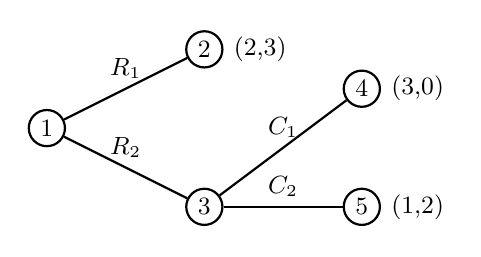
\begin{tikzpicture}[thick,
    p/.style={circle,draw,thick,inner sep=2pt,font=\small},
    out/.style={font=\small},
    opt/.style={above,font=\small},
    every label/.style={font=\small}]
  \node[p] (1) at (0,0) {1};
  \node[p,label=right:{(2,3)}] (2) at (2,1) {2};
  \node[p] (3) at (2,-1) {3};
  \draw (1) -- node[opt] {$R_1$} (2);
  \draw (1) -- node[opt] {$R_2$} (3);
  \node[p,label=right:{(3,0)}] (4) at (4,0.5) {4};
  \node[p,label=right:{(1,2)}] (5) at (4,-1) {5};
  \draw (3) -- node[opt] {$C_1$} (4);
  \draw (3) -- node[opt] {$C_2$} (5);
\end{tikzpicture}
\end{center}

\cmnt{%
  If nodes are connected by dotted lines, then the relevant player
  cannot tell if she is in one of those nodes at which of them she
  is. Such nodes form an \emph{information set}. Games in which there
  can be ignorance about the present node are said to have
  \emph{imperfect information}.%
} %

From a decision theoretic perspective, a game with several moves is a
series of (potential) decision problems, one for each occasion where a
player faces a choice. The states in these decision problems specify
the future decisions of all players. As before, under the assumption
that the utilities and rationality of players are common knowledge, we
can often predict what will happen without specifying the players'
degrees of belief.

Consider the node labelled `3' in the above tree. Here, Column faces a
choice between outcome 4 and outcome 5. That choice involves no
relevant uncertainty, and Column prefers outcome 5. So Column can be
expected to play $C_2$. Anticipating this, Row can figure out that if
she plays $R_2$, then outcome 5 will come about, which has utility 1
for Row. By comparison, if she plays $R_1$, she guarantees outcome 2,
which has utility 2. So Row will play $R_1$.

This process for solving games with multiple moves is called
\textbf{backward induction}. It can lead to very strange results.

\cmnt{%

  A game tree can be reduced to a simple decision matrix by pretending
  that all players decide at the outset on a \emph{strategy} that
  settles what they will choose at each point they might reach, with
  the constraint that the same choice must be made at each point in an
  information set. The resulting matrix is known as the
  \emph{strategic normal form} of the game tree.

  The outcome of an interaction often depends not only on their
  individual choices, but also on external matters, e.g. on whether
  some restaurant is open. Game theory accommodates this by using
  ``lotteries'' as outcomes. For instance, if I want to meet you, and
  we both end up at the restaurant, the outcome might be the complex
  state of affairs $\bet{\emph{Open}}{\emph{Meet \& Eat}}{\emph{Meet
      \& $\neg$Eat}}$. The utility of this state of affairs then
  depends on the probability that the restaurant is open. Since game
  theory tries to avoid specifying subjective probabilities, it is
  usually assumed that the relevant events have an objective chance
  which is common knowledge among all players. Thus it might be
  specified that all parties know that the restaurant owner each day
  decides whether to open her restaurant based on a fair coin toss.

  It's important to treat such games not in normal form. That's
  because the normal form ignores information that can arrive during a
  game. In particular, an agent might play something unexpected and
  this might change what the other agent should do.
} %

\begin{example}[Centipede]
  You and Bob are playing a game. Initially, there's a pot containing
  £2. In round 1, you begin by deciding whether to continue or end the
  game. If you end the game, you get the £2 and Bob gets £0. If you
  continue, the money in the pot increases by £2 and Bob decides
  whether to continue or end. If he ends the game here (in round 2),
  he gets £3 and you get £1. If he continues, the money in the pot
  increases by £2 and it's your turn again. If you end the game 
  (in round 3), you get £4 and Bob gets £2. And so on. In each round,
  the money in the pot increases by £2 and whoever ends the game gets
  £2 more than the other player. In round 100, Bob no longer has an
  option to continue.
\end{example}

Now suppose you and Bob only care about how much money you get from
the Centipede game. Here is a partial diagram.

\begin{center}
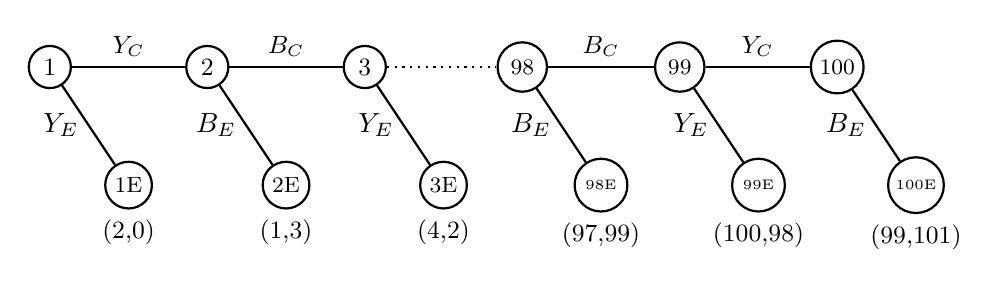
\begin{tikzpicture}[thick,
    p/.style={circle,draw,thick,inner sep=2pt,font=\small},
    xp/.style={circle,draw,thick,inner sep=2pt,font=\footnotesize},
    xxp/.style={circle,draw,thick,inner sep=2pt,font=\tiny},
    out/.style={font=\small},
    opt/.style={above,font=\small},
    every label/.style={font=\small}]
  \node[p] (1) at (0,0) {\,1\,};
  \node[xp,label=below:{(2,0)}] (1E) at (1,-1.5) {1E};
  \draw (1) -- node[left] {$Y_E$} (1E);
  \node[p] (2) at (2,0) {\,2\,};
  \node[xp,label=below:{(1,3)}] (2E) at (3,-1.5) {2E};
  \draw (2) -- node[left] {$B_E$} (2E);
  \draw (1) -- node[opt] {$Y_C$} (2);
  \node[p] (3) at (4,0) {\,3\,};
  \node[xp,label=below:{(4,2)}] (3E) at (5,-1.5) {3E};
  \draw (3) -- node[left] {$Y_E$} (3E);
  \draw (2) -- node[opt] {$B_C$} (3);
  \node[xp] (98) at (6,0) {\,98\,};
  \node[xxp,label=below:{(97,99)}] (98E) at (7,-1.5) {\,98E\,};
  \draw (98) -- node[left] {$B_E$} (98E);
  \draw[dotted] (3) -- (98);
  \node[xp] (99) at (8,0) {\,99\,};
  \node[xxp,label=below:{(100,98)}] (99E) at (9,-1.5) {\,99E\,};
  \draw (99) -- node[left] {$Y_E$} (99E);
  \draw (98) -- node[opt] {$B_C$} (99);
  \node[xp] (100) at (10,0) {100};
  \node[xxp,label=below:{(99,101)}] (100E) at (11,-1.5) {100E};
  \draw (100) -- node[left] {$B_E$} (100E);
  \draw (99) -- node[opt] {$Y_C$} (100);
\end{tikzpicture}
\end{center}

We can use backward induction to figure out how you should play. The
latest point at which a player has a real choice is round 99. Here,
you can either end the game ($Y_E$) and get £100 or continue ($Y_C$)
and get £99. So you should end the game. Anticipating this, what
should Bob do in round 98? If he ends the game ($B_E$), he'll get £99;
if he continues ($B_C$), he'll get £98. So he should end the
game. Anticipating this, you should end the game in round 97, to
ensure that you'll get £98 rather than £97. And so on, all the way
back to round 1. At each point, backward induction tells us the game
should be ended. Thus knowing at round 1 that Bob will end the game in
round 2, you should end the game right away. So the ``solution'' is
that you will get £2 and Bob gets £0.

\begin{exercise}
  Can you think of a real-life situation with a structure similar to
  the centipede game? $\star\star$
\end{exercise}

When actual people play the Centipede game, almost no-one ends the game
right away. Is this a sign of irrationality? Not necessarily.

Let's look at your choice in round 1 from a decision theoretic
perspective. It is clear what happens if you end the game: you'll get
£2. But what would happen if you decide to continue? The argument from
backward induction assumes that Bob would end the game. And if you
could be certain that Bob would do that, then you should indeed end
the game in round 1. But why should Bob end the game? Because, so the
argument, he can be certain that you would end the game in round
3. But the argument for ending in round 3 is exactly parallel to the
argument for ending in round 1. Yet if Bob faces a choice in round 2,
then he has just seen that you \emph{didn't} end the game in round
1. So he arguably can't be sure you would end it in round 3. On the
contrary, he should be somewhat confident that you will continue in
round 3. And then Bob should continue in round 2. Crucially, if all
that is right, then continuing in round 1 maximizes expected utility,
as it is likely to get you at least to round 3!

\cmnt{%

  is what you would do if I were to play the ``wrong'' move. You would
  learn that either I'm not rational, or you're wrong about the
  utilities, or I believe that you're not rational or that you're
  wrong or that you believe that I'm wrong etc.

} %

\begin{exercise}
  Change the Centipede game so that there's no fixed end
  point. Rather, each time a player chooses to continue, the game ends
  with a probability of 1\%. Does this change anything? How should
  you play? $\star\star$
\end{exercise}

\begin{exercise}
  Suppose you repeatedly face a Prisoner Dilemma against the same
  opponent, for an unknown number of rounds. You expect that your
  opponent will remain silent in the first round and from then on
  imitate whatever you will do. Given that, it seems reasonable that
  you should remain silent. Does that mean you should choose an act
  that doesn't maximize expected utility? $\star\star$
\end{exercise}


\section{Evolutionary game theory}

\cmnt{%
  Here we are in effect imposing external utilities: we're not
  interesting in the agent's goals, but in what she ought to do in
  order to maximize fitness; in light of information = random or
  correlated pairing.%
} %

One of the most successful applications of game theory lies (somewhat
surprisingly) in the study of biological and cultural
evolution. Consider the following game.

\begin{example}[The Stag Hunt]
  Two players independently decide whether to hunt stag or rabbit.
  Hunting stag requires cooperation, so if only one of the players
  decides to hunt stag, she will get nothing. The utilities are as
  follows.
  \begin{center}
    \begin{tabular}{|r|c|c|}\hline
      \gr & \gr Stag & \gr Rabbit \\\hline
      \gr Stag & 5,5 & 0,1 \\\hline
      \gr Rabbit & 1,0 & 1,1 \\\hline
    \end{tabular}
  \end{center}
\end{example}
\cmnt{%
  Using standard ideas from game theory, we would find the two Nash
  equilibria (Stag,Stag), (Rabbit,Rabbit), which is not much of a
  ``solution''. %
} %

In the evolutionary interpretation, the utilities represent the
\emph{relative fitness} that results from a combination of choices,
measured in terms of average number of surviving offspring. Let's
assume that each strategy is played by a certain fraction of
individuals in a population. Individuals who achieve an outcome with
greater utility will, by definition, have more offspring on average,
so their proportion in the population will increase.

Suppose initially \nicefrac{1}{4} of the individuals in the population
goes for stags and \nicefrac{3}{4} for rabbits. Assuming that
encounters between individuals are completely random, this means that
any given individual has a \nicefrac{1}{4} chance of playing with
someone hunting stag, and a \nicefrac{3}{4} chance of playing with
someone hunting rabbit. The average utility of hunting stag is
therefore $\nicefrac{1}{4} \cdot 5 + \nicefrac{3}{4} \cdot 0 = 1.25$;
for hunting rabbit the utility is of course 1. Individuals going for
stag therefore have greater average fitness. Their fraction in the
population increases. As a consequence, it becomes even more
advantageous to go for stag. Eventually, everyone will hunt stag.

By contrast, suppose initially only \nicefrac{1}{10} of the population
goes for stags. Then hunting stag has an average utility of 0.5, which
is less than the utility of hunting rabbit. So the rabbit hunters will
have more offspring, which makes it even worse to hunt
stags. Eventually, everyone will hunt rabbits.

The two outcomes (Stag,Stag) and (Rabbit,Rabbit) are the two Nash
Equilibria in the Stag Hunt. Evolutionary game theory predicts that
the proportion of stag and rabbit hunters in a population will
approach one of these equilibria. 

\cmnt{%
  Notice that unlike in standard game theory, we made no assumptions
  about common knowledge here. The players don't have to know
  anything, and they can be quite irrational. That's because it's not
  the \emph{players} who decide which strategy is optimal and which
  equilibrium will be reached, but \emph{nature}. Individuals aren't
  actually trying to maximise fitness, but they nevertheless behave as
  if they were, because nature selects for individuals with higher
  fitness.
} %

\cmnt{%

  If you think of all possible fractions of strategies as a phase
  space, the equilibrium (Stag, Stag) has a larger basin of attraction
  than (Rabbit, Rabbit). Sometimes, a Nash equilibrium has a
  point-sized basin of attraction, such as $B,B$ in the following
  game:

  \begin{center}
    \begin{tabular}{|r|c|c|}\hline
      \gr & \gr A & \gr B \\\hline
      \gr B & 5,5 & 0,0 \\\hline
      \gr B & 0,0 & 0,0 \\\hline
    \end{tabular}
  \end{center}

  It is very unlikely that this equilibrium could ever be found -- not
  only because it is unlikely that all players start off playing
  B. Rather, even in this case, mutants or intruders playing A will
  quickly take over. 

} %

Not every Nash Equilibrium is a possible end point of evolution
though. For example, if a population repeatedly plays the game of
Chicken, and the players can't recognize in advance who will swerve
and who will go straight, then the asymmetric equilibria (Swerve, Straight)
and (Straight, Swerve) do not mark possible end points of evolutionary
dynamics. But note that in a community in which almost everyone
swerves, you're better off going straight; similarly, in a community
in which almost everyone goes straight, the best choice is to
swerve. Evolution will therefore lead to the third, mixed strategy
equilibrium, which represents a state in which a certain fraction of
the population swerves and the others go straight.

\cmnt{%
  Hunting stag and hunting rabbit are \textbf{evolutionarily stable}
  in the sense that mutants playing the alternative strategy could not
  take over a population of 100\% stag hunters or 100\% rabbit
  hunters.
} %

\cmnt{%
  for all other strategies $Y$,
  \begin{itemize}
  \item \emph{either} $U(X,X) > U(Y,X)$,
  \item \emph{or} $U(X,X) = U(Y,X)$ and $U(X,Y) > U(Y,Y)$.
  \end{itemize}
  The idea is that either $X$ is \emph{strictly} better against itself
  than every alternative, or, if some mutant alternative $Y$ does
  equally good against $X$, then $X$ does better against $Y$ than $Y$
  itself. 
} %

\cmnt{%
  Considerations of mutants and invaders point at a limitation of our
  original dynamical model, which assumed that the ratios in the next
  generation are entirely determined by the ratios in the parent
  generation and their fitness, without mutation and invasion. There are
  more complex models including these factors.

  Notice that unlike in standard game theory, we made no assumptions
  about common knowledge here. The players don't have to know
  anything, and they can be quite irrational. That's because it's not
  the \emph{players} who decide which strategy is optimal and which
  equilibrium will be reached, but \emph{nature}. Individuals aren't
  actually trying to maximise fitness, but they nevertheless behave as
  if they were, because nature selects for individuals with higher
  fitness.

  What exactly is fitness in evolutionary game theory? It is best
  defined by its role: fitness is something such that the more you
  have it, the more creatures like you will exist in the next
  generation. An obvious candidate is number of offspring, but there
  are situations where this isn't adequate, e.g. when the players are
  ants or more generally when players have a choice that helps other
  players of their type to have more offspring. Biologists sometimes
  speak of ``inclusive fitness'' to take such factors into account.
} %

The assumption that individuals in a population are randomly paired
with one another is obviously unrealistic. In reality, individuals are
more likely to interact with members of their own family, which
increases the chances that they will be paired with individuals of the
same type; they might also actively seek out others who share the
relevant traits. Either way, the resulting \textbf{correlated play}
dramatically changes the situation.

For example, consider a population in which individuals repeatedly
play a Prisoner Dilemma wherein they can either cooperate with each
other (remain silent, in the original scenario) or defect
(confess). Since defectors always do better than cooperators in any
encounter, it may seem that cooperation can never evolve. However,
cooperators do much better when paired with other cooperators than
defectors when paired with defectors. If the extent of correlation is
sufficiently high, cooperators can therefore take over (although
perhaps not completely). 

In many species, one can find altruistic individuals who sacrifice
their own fitness for the sake of others. Evolutionary game theory
explains how this kind of altruism could have evolved.

\begin{exercise}
  Why can't we expect cooperative behaviour to take over completely in
  the scenario where cooperation spreads through correlated play?
  $\star$
 \end{exercise}

\begin{exercise}
  What are the Nash equilibria in the following game (ignoring
  randomization)? Could all the equilibria come about through an
  evolutionary process? $\star$
  \begin{center}
    \begin{tabular}{|r|c|c|}\hline
      \gr & \gr A & \gr B \\\hline
      \gr A & 5,5 & 1,1 \\\hline
      \gr B & 1,1 & 1,1 \\\hline
    \end{tabular}
  \end{center}
\end{exercise}

\section{Further reading}

The Stanford Encyclopedia entry on game theory provides a fairly comprehensive overview:

\begin{itemize}
\item Don Ross: \href{https://plato.stanford.edu/entries/game-theory/}{``Game Theory''} (2014)
\end{itemize}

The paradox of backward induction is discussed in
\begin{itemize}
\item Philip Pettit and Robert Sugden: \href{https://www.princeton.edu/~ppettit/papers/BackwardInduction_JournalofPhilosophy_1989.pdf}{``The Backward Induction Paradox''} (1989)
\end{itemize}

For a little more on evolutionary game theory, see

\begin{itemize}
\item Brian Skyrms: ``Game Theory, Rationality and Evolution of the Social Contract'' (2000) 
\end{itemize}

\begin{essay}
  Explain the paradox of backward induction. Why is it a paradox? How
  do you think it could be resolved?
\end{essay}


%%% Local Variables: 
%%% mode: latex
%%% TeX-master: "bdrc.tex"
%%% End:
\chapter{Bounded Rationality}

\section{Models and reality}

We have studied an abstract model of rational agents. The model
assumes that the agent to be modelled has some idea of what the world
might be like, which we represent by a credence function $\Cr$ over a
suitable space of propositions. We also assume that the agent has some
goals or values or desires, which we represent by a utility function
$U$ on the same space of propositions. The credence function is
assumed to satisfy the formal rules of the probability calculus; it is
assumed to evolve over time by conditionalizing on sensory
information, and it is assumed to satisfy further constraints such as
the Probability Coordination Principle. The utility function $U$ is
assumed to satisfy Jeffrey's axiom, so that it is jointly determined
by the agent's credences and the basic values assigned to individual
possible worlds. The basic values may in turn be determined by
aggregating subvalues. When the agent faces a choice, she is assumed
to choose an act which maximizes the credence-weighted average of the
utility of the act's possible outcomes.

As we saw, the model is really a family of models, since there are
different ways of filling in the details. Should expected utility be
understood causally or evidentially? Should credences satisfy a
restricted version of the Principle of Indifference? Should utilities
conform to localism?  Should they be stationary? And so on.

Each model in this family can be understood either
\textbf{normatively} or \textbf{descriptively}. Understood
normatively, the models purport to describe an ideal which real agents
should perhaps aspire to. Understood descriptively, the models purport
to describe the attitudes and choices of ordinary humans.

It is a commonplace in current economics and psychology that our
models are descriptively inadequate: that real people are not expected
utility maximizers. In itself, this is not necessarily a problem --
not even for the descriptive interpretation of the models. Remember
that ``all models are false''. With the possible exception of the
standard model of particle physics, the purpose of a model is to
identify interesting and robust patterns in the phenomena, not to get
every detail right.  Nonetheless, it is worth looking at how real
agents fail to conform to our models, and what we could change to make
the models more realistic.

Many examples of people supposedly failing to maximize expected
utility are not really counterexamples to the descriptive adequacy of
our models, since the examples rely on implausible restrictions on the agent's
utility function. As we saw in session \ref{ch:risk}, our models can easily
accommodate agents who care about risk or fairness or feelings of
frustration, which explains the common preferences in Allais's
paradox. We can similarly accommodate altruistic behaviour (section
\ref{sec:decision-matrices}), the endowment effect (section
\ref{sec:sources-utility}), or apparent failures of time consistency
(section \ref{sec:separability-time}).

\cmnt{%
  Another fact is that preference orders themselves can vary. They
  clearly vary across long stretches of time: my favourite food is no
  longer what it used to be when I was seven. (We could say that my
  preference is still the same, for I still prefer eating pasta and
  being seven to eating brussels sprouts and being seven, but it is
  not clear that anything is gained from that.) They can also vary in
  shorter intervals -- from morning to evening, from talking to a
  pretty woman to no longer talking to her. Here again we need
  substantive constraints to divide these into ``rational'' changes
  and ``irrational'' changes, and the borderline is fuzzy.
} %

But other phenomena are harder to accommodate. For example, suppose I
offer you £100 for telling me the prime factors of 82717. You have 10
seconds. Can you do it? Probably not. All you'd have to do to get the
money is utter `181 and 457'. You plausibly know that `181 and 457' is
the correct answer just in case the prime factors of 82717 are 181 and
457. And as an ideal Bayesian agent, you should be confident that the
prime factors of 82717 are 181 and 457. To maximize expected utility
(assuming you'd like to get the £100), you should therefore utter `181
and 457'. Yet you don't.

\begin{exercise}
  Why should you be confident, as an ideal Bayesian agent, that the
  prime factors of 82717 are 181 and 457? $\star$
\end{exercise}

In 1913, Ernst Zermelo proved that in the game of chess, there is
either a strategy for the starting player, White, that guarantees
victory no matter what Black does, or there is such a strategy for
Black, or there is a strategy for either play to force a
draw. Consequently, if two ideal Bayesian agents sat down to a game of
chess, and their only interest was in winning, they would
immediately agree to a draw or one of them would resign before the
first move. Real people don't play like that.

Another obvious respect in which real people deviate from the Bayesian
ideal is that real people often forget. In section \ref{sec:why-meu},
I mentioned forgetting to buy soap in the shop. That's a temporary
kind of forgetting, because you later remember what you forgot. We
also often lose information completely. As an ideal Bayesian agent,
you would still know what you had for breakfast on 12 June 2006.

\begin{exercise}
  Show that if $\Cr_t(A) = 1$, and the agent conditionalizes on
  information $E$ with $\Cr_t(E) > 0$, then $\Cr_{t+1}(A) =
  1$. (Conditionalization was introduced in
  section \ref{sec:conditionalization}.) $\star$
\end{exercise}

\cmnt{%
  Other issues are less clear. E.g., it is widely claimed that real
  agents are not ``logically omniscient'', meaning that they are not
  certain of every logical truth, in violation of Kolmogorov's axiom
  2. But it is not obvious what it would mean for an agent to have
  credence less than 1 in a logical truth, and therefore it is also
  not obvious whether people actually have such attitudes. Indeed, if
  `credence' is a technical term defined by our model, then so far it
  is trivially true that everyone is logically omniscient. We would
  need an alternative model.
} %

So it's plausibly true that our model doesn't fit real agents in
certain respects. As we are going to see, there is indirect evidence
for this from research on artificial intelligence. The type of model
we have studied is well known in these quarters, and forms the
background for much recent research.%
\cmnt{%
  see RN.%
} %
Yet the model turns out to be computationally intractable. Real agents
with limited cognitive resources, it seems, couldn't possibly conform
to our models.


\section{Avoiding computational costs}

Before we look at ways of making our models more realistic, I want to
address another common misunderstanding.

Suppose you walk back to shop to buy soap. At any point on your way,
you could decide to turn around, or start running, or check if your shoe
laces are tied, or mentally compute $181 + 457$, or start humming the
national anthem, or utter `Age quod agis', and so on. There are
literally millions of things you could do. Many of these would lead to
significantly different outcomes, especially if you consider long-term
consequences. (Hitler almost certainly would not have existed if hours
or even months before his conception, his mother had decided to run
rather than walk to buy soap.) Some people take the MEU Principle to
imply that at each point of your walk to the shop, you should
explicitly consider all your options, envisage all their possible
outcomes, assess their utility and probability, and on that basis
compute their expected utility. Real people clearly don't do that.

But the MEU Principle requires no such thing. The MEU Principle says
that rational agents choose acts that maximize expected utility; it
says nothing about the internal process that leads agents to these
choices. It definitely doesn't say that the agent must explicitly
consider all her options and compute expected utilities.

The opposite is closer to the truth. If an agent has the capacity to
compute the expected utility of all her options, then the MEU
Principle generally says that the agent should \emph{not} exercise
that capacity. (If an agent does not have the capacity, so that
computing expected utilities is not even an available act, the MEU
Principle obviously also doesn't say that the agent should carry out that act.)

The reason is simple. Let $A_1,\ldots,A_n$ be your ``basic'' options,
those that don't involve computing expected utilities. In addition to
these, we assume, you have the option $C$ of computing the expected
utilities of $A_1,\ldots,A_n$ and then choosing whichever of them
comes out best. Let $A_i$ be the best of the basic options. If you
choose $C$, you are guaranteed to get the same outcome as if you
choose $A_i$ directly, except that you've also spent some time and effort
on computing expected utilities. Usually, that will ensure that
whatever outcome you get from $C$ is worse than what you would have
gotten from $A_i$. Thus $A_i$ has greater expected utility than $C$,
and you should not choose $C$.

\begin{exercise}
  The argument just outlined is not fully general. There are unusual
  cases in which $C$ would have greater expected utility than directly
  choosing $A_i$, even though the computation has negative
  (sub)value. What do such cases look like? $\star\star$
\end{exercise}

\cmnt{%
  So unless they get some direct value from computing expected
  utilities, ideal Bayesian agents don't compute expected
  utilities. Instead they directly choose whichever option maximizes
  expected utility.
  
  That may seem strange. How is the agent supposed to arrive at her
  choice of the best option, if not by figuring out that it maximizes
  expected utility? By accident? That doesn't look rational. By magic?
  
  Part of the answer is that ideal Bayesian agents have no need to
  compute anything: if they are certain of some facts, and these facts
  entail other facts, then the probability axioms entail that they are
  also certain of the other facts. For ideal Bayesian agents,
  computations are a costly process of arriving at results that are
  already known.
} %

So ideal Bayesian agents generally don't compute expected
utilities. That may seem puzzling. How can you reliably choose an
act with greatest expected utility if you don't compute expected
utilities?

One possibility is that you \emph{already know} which acts maximize
expected utility, without any computations. But there are other, more
realistic possibilities. The psychologist Gerd Gigerenzer once pointed
out that if you want to catch a flying ball, an efficient strategy is
to move around in such a way that the angle between you and the ball
remains within a certain range. This is much easier than explicitly
computing the ball's trajectory, and it ensures that you'll eventually
stand where the ball will arrive. The point is that in order to
reliably achieve a goal, you can often fall back on simple
heuristics. If you desire to catch the ball, following Gigerenzer's
heuristic will maximize expected utility. You don't need to explicitly
compute anything.

In addition, many decision problems don't require computing expected
utilities because one act clearly dominates. Whether that is the case
depends on the agent's utility function. So you can often reduce the
computational costs of decision-making by tweaking your utilities. For
example, suppose you assign significant (sub)value to obeying
orders. Doing whatever you're ordered to do is then a reliable way of
maximizing expected utility, and it requires very little cognitive
effort. Similarly if you value imitating whatever your peers are
doing.

\cmnt{%
  Endowing individuals with a desire for social conformity might be an
  evolutionary trick to ensure that people make reasonably simple
  choices without having to reason too much. (Conformity has other
  evolutionary advantages as well.)
} %

Our capacity for planning and commitment can also be seen in this
light. Before you went to the shop, you probably decided to go to the
shop. The result of that decision was in the first instance an
intention to go to the shop.

\cmnt{%
  Somewhat confusingly, according to our model, this was not a
  decision to go to the shop. That's because, at the time, going to
  the shop was not strictly speaking an available act, since was
  partly outside your control. Someone could have prevented you from
  leaving the house. You could have gotten into an accident while
  crossing the street. Your future self could have been seduced by the
  sight of the pub and stopped for a few beers. When you decided to go
  to the shop, the ``act'' you chose was an act of commitment or
  planning. You formed the intention of going to the shop.%
} %

Once an intention or plan if formed, we assign value to executing the
plan. Revising a plan or overturning a commitment has negative
(sub)value. As a result, if you've formed a plan, simply following it
often reliably maximizes expected utility. You don't need to think any
more about what to do unless you receive surprising new information or
your basic values suddenly change.

Habits can play a similar role. Most of us spend little effort
deciding whether or not to brush our teeth in the morning; we do it
out of habit. Habitual behaviour is computationally cheap, and it can
reliably maximize expected utility -- especially if we assign
(sub)value to the habitual behaviour. And we do, at least on a
motivational conception of desire: habits motivate.

The upshot is that various cognitive strategies that are often
described as alternatives to computing expected utilities -- habits,
instincts, heuristics, etc.\ -- may well be efficient
techniques for maximizing expected utility. Far from ruling out such
strategies, our model actually predicts that we should use them.

\cmnt{%
  Still, one might complain that our model lacks detail.  We could
  model pointless habitual behaviour as simply MEU, but to understand
  why someone might have the relevant utilities, it is useful to
  develop a more complex model that distinguishes between deliberate
  and habitual behaviour. (Such ``two systems'' models are common both
  in psychology and neuroscience; see e.g.\ Dickinson A. Actions and
  habits: the development of behavioural autonomy. Philosophical
  Transactions of the Royal Society B: Biological Sciences. 1985;
  308:67–78 and 2 system theory.)
} %

A famous example in which something like this might play a role is
Ellsberg's Paradox.

\begin{example}[Ellsberg's Paradox]
  An urn contains a red ball and two other balls. The other balls have
  been selected from a box containing only green and blue balls, but
  you don't know which colours where chosen. A ball is drawn at random
  from the urn. Which of the following two lotteries do you prefer?
  % 
  \begin{center}
  \begin{tabular}{|r|c|c|c|}\hline
    \gr & \gr Red & \gr Green & \gr Blue \\\hline
    \gr $A$ & £1000 & £0 & £0 \\\hline
    \gr $B$ & £0 & £1000 & £0  \\\hline
  \end{tabular}
  \end{center}
  %
  Next, which of $C$ and $D$ do you prefer?
  % 
  \begin{center}
  \begin{tabular}{|r|c|c|c|}\hline
    \gr & \gr Red & \gr Green & \gr Blue \\\hline
    \gr $C$ & £1000 & £1000 & £0 \\\hline
    \gr $D$ & £0 & £1000 & £1000 \\\hline
  \end{tabular}
  \end{center}
\end{example}

Many subjects prefer $A$ to $B$ and $D$ to $C$. Like in Allais's
Paradox, there is no way of assigning utilities to the monetary
outcomes that supports these preferences.

In Ellsberg's Paradox, risk aversion doesn't seem to be at issue. What
makes the difference is that you know the objective probability of
winning for options $A$ and $D$: it is \nicefrac{1}{3} for $A$ and
\nicefrac{2}{3} for $D$. But you don't know the objective probability
of winning with $B$ and $C$, since you have too little information
about the non-red balls. 

Why does that matter? One explanation is that people simply prefer
lotteries (in which the outcomes have known objective
probabilities) to uncertain prospects (in which only subjective
probability can be given to the outcomes). With such a utility
function, the outcome wrongly labelled `£1000' in $A$ is actually
better than the corresponding outcome in $C$, because only the former
involves having chosen a lottery.

\begin{exercise}
  The explanation of the Ellsberg preferences that I just outlined
  makes the preferences conform to the MEU Principle by redescribing
  the outcomes. Is the redescription global or local in the sense of
  session \ref{ch:risk}? $\star$
\end{exercise}

But why would agents prefer lotteries? Perhaps because such a
preference can reduce computational costs. If you know the objective
probabilities of the outcomes, it is easy to figure out the credence
you should give to the outcomes: it should match the objective
probabilities. If you don't know the objective probabilities, a lot
more work may be required to figure out the extent to which your total
evidence supports the occurrence of the various outcomes. In
Ellsberg's Paradox, $\Cr(\text{Red})$ is a easier to figure out than
$\Cr(\text{Green})$ and $\Cr(\text{Blue})$. If you have a preference
for lotteries, you don't need to figure out $\Cr(\text{Green})$ and
$\Cr(\text{Blue})$: from eyeballing the options, you can already see
that the expected monetary payoff of $A$ and $B$ is approximately the
same (ditto for $C$ and $D$); a preference for lotteries then clearly
favours $A$ (and $D$).


\section{Reducing computational costs}

I will now review a few ideas from theoretical computer science for
rendering our models computationally tractable.

Imagine we are designing an artificial agent, with a probabilistic
representation of her environment and a number of goals or
desires. Let's assume we want the agent to have credences and
utilities in 50 logically independent propositions
$A_1,\ldots,A_{50}$ (an absurdly small number).
How large of a database do we need for that?

You might think that we need 50 records for the probabilities and 50
for the utilities. But we generally can't compute $Cr(A \land B)$ or
$\Cr(A \lor B)$ from $\Cr(A)$ and $\Cr(B)$. Nor can we compute $U(A
\land B)$ or $U(A \lor B)$ from $U(A)$ and $U(B)$. In order to fix the
agent's entire credence and utility functions (without further
assumptions about these functions), we need to store at least the
probability and utility they assign to every ``possible world'' --
that is, to every maximally consistent conjunction of
$A_1,\ldots,A_{50}$ and their negations.

\begin{exercise}
  Explain why the probability of every proposition that can be defined
  in terms of $A_1,\ldots,A_{50}$ can be computed from the probability
  assigned to the possible worlds. Then explain why the utility of all
  such propositions can be computed from the probability and utility
  assigned to the worlds. $\star\star$
\end{exercise}

\cmnt{%
  Since every proposition that can be defined in terms of
  $A_1,\ldots,A_{50}$ is equivalent to a disjunction of these possible
  worlds, Kolmogorov's axiom (iii) and Jeffrey's Axiom ensure that we
  can compute all probabilities and utilities from the assignment to
  possible worlds.
} %

There are $2^{50} = 1,125,899,906,842,624$ maximally consistent
conjunctions of $A_1,\ldots,A_{50}$ and their negations.  So we need a
database with $2,251,799,813,685,248$ records. (I'm exaggerating a
little. Once we've fixed the probability of the first
1,125,899,906,842,623 worlds, the probability of the last world is 1
minus the sum of the others, so we really only need
$2,251,799,813,685,247$ records.)

We'll need to buy a lot of hard drives for our agent if we want to
store 2 quadrillion floating point numbers. Worse, updating all these
records in response to sensory information, or computing expected
utilities on their basis, will take a very long time, and use a large
amount of energy.

In session \ref{ch:separability}, we've encountered two tricks for
simplifying the representation of an agent's basic value function --
the utility function for individual worlds. First, if the agent cares
about some features of the world and not about others, it is enough to
store the agent's value for sets of worlds that agree in all respects
that matter to the agent; all worlds within such a set will have the
same value as the set itself (section
\ref{sec:construction-value}). For example, if our agent only cares
about the possible combinations of 20 among the 50 propositions
$A_1,\ldots,A_n$, we only need to store $2^{20}$ values. Second, and
more dramatically, if the agent's preferences are separable, we can
cut down the number of utility records from $2^{20}$ to $2 \cdot 20 =
40$, because the value of any combination of the 20 propositions and
their negations can be determined by adding up the relevant subvalues
(section \ref{sec:additivity}).

Similar tricks are available for the agent's credence
function. Mirroring the first trick, we could explicitly store only
the agent's credence in certain sets of possible worlds, and assume
that her credence is distributed uniformly within these sets. The
trick can be extended to non-uniform distributions. For example,
suppose our agent has imperfect information about how far she is from
the next charging station. Instead of explicitly storing a probability
for every possible distance (1 m, 2 m, 3 m, \ldots), we might assume
that the agent's credence over these possibilities follows a Gaussian
distribution, which can be specified by two numbers (mean and
variance). Researchers in artificial intelligence make heavy use of
this trick.

An analogue of separability, for credences, is probabilistic
independence. If $A$ and $B$ are probabilistically independent, then
$\Cr(A\land B) = \Cr(A) \cdot \Cr(B)$. If all the 50 propositions
$A_1,\ldots,A_{50}$ are mutually independent,
then specifying their individual probability is enough to specify the
probability of all possible worlds and therefore of all logical
combinations of the 50 propositions.

Independence is often plausible. Whether the next charging station is
100 meters away plausibly doesn't depend on whether the outside
temperature is above 20\celsius. But for many other propositions,
independence is implausible. On the supposition that the temperature
is above 20\celsius, it may well be more likely that the window is
open, or that there are people on the street; so
$\Cr(\emph{Open}/\emph{Warm}) > \Cr(\emph{Open})$, and
$\Cr(\emph{People}/\emph{Warm}) > \Cr(\emph{People})$. So we can't
assume probabilistic independence across all the 50 propositions $A_1,\ldots,A_{50}$.

Even where independence fails, we often have \textbf{conditional independence}. For example,
if warm temperatures make it more likely that the window is open and
that there are people on the street, then an open window is also evidence
that there are people on the street: $\Cr(\emph{People}/\emph{Open}) >
\Cr(\emph{People})$.  So \emph{People} and \emph{Open} are not
independent. However, \emph{on the supposition that it is warm
  outside}, the window being open may no longer increase the
probability of people on the street:
\[
\Cr(\emph{People}/\emph{Open} \land \emph{Warm}) = \Cr(\emph{People}/
\emph{Warm}).
\]
In that case, we say that \emph{People} and \emph{Open} are
independent \emph{conditional on} \emph{Warm}.

Now consider the possible combinations of \emph{Warm}, \emph{People},
\emph{Open} and their negations. By the probability calculus
\[
\Cr(\emph{Warm} \land \emph{People} \land \emph{Open}) = 
\Cr(\emph{Warm}) \cdot \Cr(\emph{Open}/\emph{Warm}) \cdot \Cr(\emph{People}/\emph{Open} \land \emph{Warm}).
\]
By the above assumption of conditional independence, this simplifies to
\[
\Cr(\emph{Warm} \land \emph{People} \land \emph{Open}) = 
\Cr(\emph{Warm}) \cdot \Cr(\emph{Open}/\emph{Warm}) \cdot \Cr(\emph{People}/\emph{Warm}).
\]
In general, with the assumption of conditional independence, we can
fix the probability of all combinations of \emph{Warm}, \emph{People},
\emph{Open}, and their negations by specifying the probability of
\emph{Warm}, the probability of \emph{People} conditional on
\emph{Warm} and $\neg\emph{Warm}$, and the probability of \emph{Open}
conditional on \emph{Warm} and $\neg\emph{Warm}$.  This reduces the
number of required records from $2^3-1 = 7$ to 5, which may not look
all that impressive, but the method really pays off if more than three
propositions are involved.

The present technique of exploiting conditional independence to
simplify probabilistic models is known under the heading of
\textbf{Bayesian networks} (or \textbf{Bayes nets}, for short). Bayes
nets have proved useful in wide range of applications.

A special case of Bayes nets%
\cmnt{%
  called \textbf{Dynamic Decision Networks}%
} %
are commonly used in artificial intelligence to model decision-making
agents. A decision-making agent needs not only information about the
present state of the world, but also about the future. We can model a
whole history of states as a sequence $\t{S_1,S_2,S_3,\ldots}$, where
$S_1$ is a particular hypothesis about the present state, $S_2$ about
the next state, and so on. If there are 100 possible states at any
given time, there will be $100^{10} = 100,000,000,000,000,000,000$
possible histories with length 10. Instead of storing individual
probabilities for all these histories, it helps to assume that a later
state (probabilistically) depends only on its immediate predecessor,
so that $\Cr(S_3/S_1 \land S_2) = \Cr(S_3/S_2)$. This is known as the
\textbf{Markov assumption}. It reduces the number of records we'd to
store from $100^{10}$ to $990,100$.%
\cmnt{%
  $100 + (100\cdot 100)\cdot 99 \approx 1000000$ %
} %
\cmnt{%
  It also simplifies belief updates through
  conditionalization. Assuming that sensory information only carries
  direct information about the present state of the world, we only
  need to store $\Cr(E/S)$ for any evidence proposition $E$ and state
  $S$.%
} %

To further simplify the task of decision-making, computer scientists
typically assume that basic values are stationary and separable across
times, so that the value of a history of states is a discounted sum of
the subvalue for individual states. To specify the whole utility
function, we then only need to store the discounting factor $\delta$
and 100 values for the individual states. The task of
conditionalization can also be simplified, by assuming that sensory
evidence only contains direct information about the present state of
the world, rather than entire histories.

These simplifications define what computer scientists call a
`\textbf{POMDP}': a \textbf{Partially Observable Markov Decision
  Process}. There is a simple recursive algorithm for computing
expected utilities in POMDPs.%
\cmnt{%
  In the jargon of computer science, maximizing the expected long-run
  utility is called \textbf{planning}.  } %

\cmnt{%
  There is evidence that our brains do process sensory signals roughly
  in line with \eqref{Bayesint}, and evaluate actions and outcomes
  roughly in line with \eqref{EUint} (see
  \cite[296--299]{gershman12perception} for literature). Of course,
  the two components are not entirely independent (a point emphasised
  in \cite{gershman12perception}): organism have greater interest in
  learning about aspects of the world with possibly extreme (positive
  or negative) utility; thus our sensory processing is often attuned
  to what matters to us in terms of utility.
} %

\cmnt{%
  \begin{exercise}
    Explain one respect in which real decision situations are not
    adequately modelled by POMDPs.
  \end{exercise}
} %

In practice, even these simplifications generally don't suffice to
make conditionalization and expected utility maximization
tractable. Further simplifications are needed. For example, it often
helps to ``myopically'' ignore states in the distant future and let
the agent maximize the expected utility of the next $n$ states only,
for some reasonable choice of $n$. A range of other techniques have
been developed that allow an efficient \emph{approximate} computation
of expected utilities and posterior probabilities. Such techniques
are often supplemented by a meta-decision process which lets the
system choose a level of precision: when a lot is at stake, it is
worth spending more effort on getting the computations right.

\cmnt{%
  Sophisticated models have been developed that apply a kind of
  meta-decision procedure to the choice of a computational
  approximation of \eqref{Bayesint} and \eqref{EUInt}, as reviewed in
  \cite[306ff.]{gershman12perception}. Again, one can let the system
  perform meta-analyses about the amount of effort to put in,
  e.g. when to stop getting a more precise update.

  ``Metalevel analyses have been aimed at endowing computational
  systems with the ability to make expected utility decisions about
  the ideal balance between effort or delay and the quality of actions
  taken in the world. The use of such rational metareasoning plays a
  central role in decision-theoretic models of bounded rationality
  (10–14)''.

  Note that if computational cost is a form of utility then once again
  we actually don't have a violation of MEU, but that's not a very
  illuminating account. (The general picture that emerges is that our
  model is largely correct, but rather uninformative for bounded
  agents.)
} %

While originating in theoretical computer science, these models and
techniques have in recent years had a great influence on our views on
human cognition. There is evidence that when our brain processes
sensory information or decides on a motor action, it employs the same
techniques computer scientists have found useful in approximating the
Bayesian ideal. Thus it has been suggested that various quirks of
human perception and decision-making are consequences of the shortcuts
our brain uses to approximate conditionalization and computing
expected utilities.%
\cmnt{%
  The family of techniques known as \textbf{predictive processing} has
  even been taken to offer an entire new perspective on many aspects
  of human cognition.%
} %

\cmnt{%
  In computer science they are usually approximated either by Monte
  Carlo simulation or by choosing a more tractable distribution $Q$
  that is similar to $P$ (as measured by KL
  distance). \cite[302f.]{gershman12perception} reviews experimental
  findings that suggest that the brain also uses some such
  approximation. For example, abrupt changes of response over the
  course of continuous learning are well explained by an underlying
  Monte Carlo approximation for \eqref{Bayesint} and \eqref{EUint}.
} %

\cmnt{%
  An exciting aspect of these models is that they explain
  ``fallacies'' not as accidental quirks but as consequences for
  optimizing with limited resources. See e.g. Griffiths et al 2015. We
  can also explain why e.g. cognitive load or stress etc. affect
  rational choice by making it reasonable to delegate more choices to
  ``model-free'' habitual systems.

  Halpern et al. 
} %

\section{``Non-expected utility theories''}

Meanwhile, researchers at the intersection of psychology and economics
have also tried to develop more realistic models of
decision-making. The most influential of these alternatives is
\textbf{prospect theory}, developed by Daniel Kahneman and Amon
Tversky.

Prospect theory has to be understood on the background of a highly
restricted version of decision theory still popular in economics. The
highly restricted theory only deals with choices between lotteries,
with known objective probabilities. The outcomes of these lotteries
are identified with monetary wealth or commodity bundles. (Even local
feelings of frustration or regret are excluded.)  Finally, it is
assumed that agents always prefer more money or goods, with declining
marginal utility. When you find social scientists discuss ``Expected
Utility Theory'', this highly restricted theory is what they usually
have in mind. Prospect theory now proposes four main changes.

1. \textbf{Reference dependence}. According to prospect theory, agents
classify possible outcomes into gains and losses, by comparing the
outcomes with a contextually determined reference point. Outcomes
better than the reference point are modelled as having positive
utility, outcomes worse than the reference point have negative
utility.

2. \textbf{Diminishing sensitivity}. Prospect theory holds that both
gains and losses have diminishing marginal utility: the same objective
difference in wealth makes a larger difference in utility near the
reference point than further away, on either side. For example, the
utility difference between a loss of £100 and a loss of £200 is
greater than that between a loss of £1000 and a loss of £1100. This
predicts that people are risk averse about gains but risk seeking
about losses: they prefer a sure gain of £500 to a 50 percent chance
of £1000, but they prefer a 50 percent chance of losing £1000 to
losing £500 for sure.

3. \textbf{Loss aversion}: According to prospect theory, people are
more sensitive to losses than to gains of the same magnitude. For
example, the utility difference between a loss of £100 and a loss of
£200 is greater than that between a gain of £200 and a gain of
£100. This explains why many people turn down a lottery in which they
can either win £110 or lose £100, with equal probability.

4. \textbf{Probability weighting}. According to prospect theory, the
outcomes are weighted not by their objective probability, but by
transformed probabilities known as `decision weights' that are meant
to reflect how seriously people take the relevant states in their
choices. Decision weights generally overweight low-probability
outcomes. Thus probability 0 events have weight 0, probability 1
events have weight 1, but in between the weight curve is steep at the edges
and flatter in the middle: probability 0.01 events might have weight
0.05, probability 0.02 events weight 0.08, \ldots, probability 0.99
events weight 0.92. Among other things, this is meant to explain why
people play the lottery, and why they tend to pay a high price for
certainty: they prefer a settlement of £90000 over a trial in which
they have a 99\% chance of getting £100000 but a 1\% chance of
getting nothing.%
\cmnt{%
  This ``certainty effect'' turns into a ``possibility effect'' at the
  other end of the scale.%

  What is supposedly captured by probability weighting is that an
  increase from a 0\% to a 1\% chance of loss significantly taints an
  option, much more than e.g.\ an increase from 20\% to 21\%. At the
  other end of the spectrum, the difference between 99\% and 100\%
  again matters a lot, much more than that between 79\% and 80\%. We
  could make the same predictions by assuming that people have
  preferences about risks, including global features in the utility
  function.
} %
\cmnt{%
  Kahneman notes that buying a lottery ticket also buys ``the right to
  dream pleasantly of winning'', and that by buying insurance you also
  ``eliminate a worry and purchase a peace of mind''
  \cite[318]{kahneman11thinking}, but he nevertheless resists
  broadening the utility function accordingly. %
} %


Prospect theory is clearly an alternative to the simplistic economical
model mentioned above. It is not so obvious whether it is alternative
to the more liberal model we have been studying for most of this
course. Diminishing sensitivity and loss aversion certainly don't
contradict our model. Reference dependence and probability weighting
are a little more subtle.

Our model assumes that if an agent knows the objective probability of
a state, then in decision-making she will weight that state in
proportion to the known probability. Prospect theory says that real
people don't do that. If we measure an agent's credences in terms of
preferences or choices, then the decision weights of prospect theory
are the agent's credences; they play precisely the role of credences
in guiding behaviour. So prospect theory assumes that people
systematically violate the Probability Coordination Principle: their
credence in low-probability event is greater than the known objective
probability.

Studies show that this failure of coordinating credences with
objective probabilities seems to depend on how the objective
probabilities are presented. Decision weights often differ widely from
objective probabilities when the probabilities are presented verbally
(`there's a 1\% chance of success', etc.), but much less so when
people have experienced the relevant probabilities as relative
frequencies in repeated trials.%
\cmnt{%
  \cite[331]{kahneman11thinking}%
} %
This suggests that we have trouble fully understanding verbal
presentations of probabilities. Widespread mistakes like the base rate
fallacy support that suspicion.

\cmnt{%

Here prospect theory therefore seems to points towards a genuine
respect in which our model doesn't fit actual human behaviour,
although it does not offer a clear picture of how and why people go
wrong when processing verbal information about probabilities.

} %

\cmnt{%
  The mere hypothesis that people's credences deviate from objective
  probabilities in a certain way however arguably doesn't get at the
  heart of the matter. What we'd need is a more general model
  explaining the difference between verbal and non-verbal
  presentation, and the particular mistakes people make.
} %

\cmnt{%
  When you decide not to switch in Monty Hall, your credences are in
  line with your choices, but they violate other norms. Defining an
  alternative model of credence is not easy.
} %

Reference dependence may also raise a genuine challenge. Most forms of
reference dependence are harmless. We can easily allow for people who
care especially about how much they will have in comparison to what
they had before, or in comparison to what their peers have. But
sometimes, the reference point is affected by intuitively
irrelevant features of the context, and that is harder to square with
our model.

\begin{exercise}
  When people compete in sports, average performance often seems to
  function as a reference point: the effort people put in to avoid
  performing below average is higher than the effort they put in to
  exceed the average.%
  \cmnt{%
    \cite[303f.]{kahneman11thinking}.%
  } %
  Can you explain this observation by ``redescribing the outcomes''?
  $\star$
\end{exercise}


\cmnt{%
  Decision theory can also accommodate for a related fact that even
  counterfactual outcomes matter: if you choose an option $[0.9 ? \$1
  million : \$0]$, then an outcome of $\$0$ will not be regarded as
  neutral; you will be thoroughly disappointed. If there was an
  alternative sure gain, even it was quite small (say, $\$1000$), you
  will probably regret your choice. Avoidance of regret and
  disappointment are psychologically important, but cannot be
  explained by prospect theory or rational choice theory
  \cite[287f.]{kahneman11thinking}. They can easily be accommodated in
  decision theory, since they are simply part of the relevant outcome.
} %

The problematic type of reference dependence is closely related to
so-called \textbf{framing effects}. In experiments, people's choices
can systematically depend on how one and the same decision problem is
described. For example, when presented with a hypothetical situation
in which 1000 people are in danger of death, and a certain act would
save exactly 600 of them, subjects are more favourable towards the act
if it is described in terms of `600 survivors' than if it is described
in terms of `400 deaths'. In prospect theory, the difference might be
explained by a change in reference point: if the outcome is described
in terms of survivors, it is classified as a gain; if it is described
in terms of deaths, it is classified as a loss.

In principle, our liberal model could also explain the relevance of
the description. Perhaps people assign basic value to choosing options
\emph{that have been described in terms of survivors} rather than in
terms of deaths. However, on reflection, most people would certainly
deny that the verbal description of an outcome is of great concern to
them. As in the case of decision weights, a more adequate model would
arguably have to take into account incomplete grasp of a verbally
described scenario. When hearing about survivors, we focus on a
certain attribute of the outcome, on all the people who are
saved. That attribute is desirable. When hearing about deaths, a
different, and much less desirable, attribute of the same outcome
becomes salient.

\cmnt{%
  But is this a failure in decision making, and should we make room
  for it in a descriptively adequate theory of decisions? I'm not
  sure. I suspect it is rather a failure in processing the information
  about the options. Under the positive description (chance of
  success), you really do consider the outcome as more desirable than
  under the negative description. So the problem isn't that you go
  wrong when putting your beliefs and desires into actions. Rather,
  you go wrong when judging the value of a verbally described
  situation. Admittedly, the issue is subtle: your calculation of EUs
  is part of your conforming to decision theory, and isn't this where
  you made the mistake, since you didn't correctly calculate the
  utility of one of the outcomes? But perhaps the more basic reason is
  that you didn't fully understand the content of the outcome you were
  told about. It's not like you were perfectly aware of the relevant
  \emph{proposition}, but sloppy when calculating its utility. The
  presentation-dependence shows that you weren't clear about what
  exactly the outcome would involve: you heard something about success
  and imagined the good case (or the lives saved etc.) and quickly
  gave a value to that, without realizing what else is entailed by the
  presentation. This is less a failure in acting than in
  understanding.
} %

Ideal agents always weigh up all attributes of every possible
outcome. Real agents arguably don't do that, as it requires
considerable cognitive effort.%
\cmnt{%
  One of Gigerenzer's heuristics is to consider only the most
  important attribute of any given outcome.%
} %
As a result, the attributes we consider depend on contextual clues
such as details of a verbal description. Some recent models of
decision making in philosophy and psychology take this kind of
attribute selection into account.

\cmnt{%
  Christian List and Franz Dietrich have a model that involves such
  context-dependent selection of salient features.
} %

\section{Imprecise credence and utility}\label{sec:imprecise}

I'm going to toss three dice. Would you rather get £10 if the sum of
the numbers I will get is at least 10 or if all three numbers are
different? You'd probably need some time to give a final answer. You
know that the six possible results for every dice have equal
probability, and that the results are independent. But it takes some
effort to infer from that which of the two events I described is more likely.

A real agent's cognitive system can't explicitly store her credence and
utility for every proposition. It can only store a limited number of
\textbf{constraints} on credences and utilities. A constraint rules
out some credences and utilities, but not others. For example, that
outcomes of die tosses are probabilistically independent is a
constraint; it entails that the probability that three dice will land
six is the product of the probabilities for the individual dice:
$\Cr(\text{Six}_1 \land \text{Six}_2 \land \text{Six}_3) =
\Cr(\text{Six}_1)\Cr(\text{Six}_2)\Cr(\text{Six}_3)$, but it does not
fix what these probabilities are.

So far, we have assumed that taken together, the constraints stored by
an agent's cognitive system are rich enough to determine a unique
credence and utility function. But maybe they don't.  Maybe there are
questions on which you don't have a settled opinion even on
reflection. Or suppose you don't have time for lengthy reflection, or
you're too tired.  In such cases, it would arguably be wrong to model
your attitudes in terms of a single, precise credence function, and a
single, precise utility functions.

Across several disciplines, researchers have developed models that
relax the assumption of precise credences and utilities. The standard
approach is to use \textbf{sets of credence and utility functions}
instead of single functions. The functions in the set are all those
that meet the constraints. Intuitively, each member of the set is a
\emph{refinement} or \emph{precisification} of the agent's
indeterminate state of mind.

The use of sets of credence functions is often motivated by
consideration like the following. How likely do you think it is that
it will snow in Toronto on 7 January 2041? If someone suggested the
probability is 80\%, you might say that's too high; 5\% seems too
low. But 20\% might seem just as plausible to you as 21\%. It would
therefore be wrong to model your state of mind by single and precise
probability. Rather, we should say that your credence is a whole range
of numbers:
\[
\Cr(\emph{Snow}) = [0.1, 0.5].
\]
Here, `$[0.1, 0.5]$' denotes the range of all numbers from 0.1 to 0.5;
it is the range of all numbers your refined credence functions assign
to \emph{Snow}.

\cmnt{%
  Suppose you similarly haven't made up your mind about whether
  Leonardo da Vinci liked porridge: $\Cr(\emph{Porridge}) =
  [0.2,0.7]$. Nonetheless, you might reasonably treat the two
  propositions as independent. (That might be one of the constraints
  encoded in your belief state.) If we model your beliefs in terms of
  credence intervals, we seem to lose the information about
  independence.%
  \cmnt{%
    Recall that \emph{Snow} and \emph{Porridge} are probabilistically
    independent just in case $\Cr(\emph{Snow}/\emph{Porridge}) =
    \Cr(\emph{Snow})$. Plausibly, $\Cr(\emph{Snow} \land
    \emph{Porridge}) = [0.01,0.25]$, so by the ratio formula, we'd
    need to assume that $\frac{[0,01,0.25]}{[0.2,0.7]} = [0.1,0.5]$.%
  } %
} %

You should be skeptical about this line of argument. The term
`probability' in English almost always means objective
probability. When asked about the probability of \emph{Snow}, it is
therefore natural to interpret the question as concerning a certain
objective quantity -- something you could perhaps find out by
developing a sophisticated weather model. But credence, on the
Bayesian conception, is not belief about objective probability. It is
simply strength of belief. You could not find out your credence in
\emph{Snow} by developing a sophisticated weather model.

Nonetheless, there are reasons to extend the Bayesian conception of
credence to allow for sets of credence functions. For example, suppose
we measure (or define) an agent's credences and utilities in terms of
her preferences. Various representation theorems show that if the
agent's preferences satisfy certain axioms, then the preferences are
represented by a \emph{unique} credence and utility function (except
for the conventional choice of zero and unit for utilities). Giving up
uniqueness then means that the agent violates one or more of the
axioms. And it is not implausible that real agents do violate some of
these axioms.

In particular, consider the completeness axiom. Completeness states
that for any propositions $A$ and $B$, the agent either prefers $A$ to
$B$ or $B$ to $A$ or is indifferent between the two. This is trivial
if we define preference in terms of choice. Indeed, presented with a
forced choice between $A$ and $B$, you will inevitably choose either
$A$ or $B$; even indifference can be ruled out. But we've already seen
that if we want to measure credence and utility in terms of
preference, then the relevant preference relation can't be directly
defined in terms of choices. And once we take a step back from choice
behaviour, it seems perfectly possible that you might neither prefer
$A$ to $B$, nor $B$ to $A$, and yet you're not indifferent between the
two. Instead, you haven't fully made up your mind. The two
propositions seem roughly ``on a par'', but you wouldn't say they are
exactly equal in value.

For example, would you rather lose your capacity to hear or your
capacity to walk? You may well have no clear preference, even after
considerable reflection. Does that mean you're exactly indifferent?
Not necessarily. If you were, you should definitely prefer losing the
capacity to hear \emph{and getting £1} to losing the capacity to
walk. In reality, the added £1 probably doesn't make any difference.

\begin{exercise}
  Suppose we define `$\sim$' in terms of `$\succ$', as follows: $A\sim
  B \Leftrightarrow (A \not\succ B) \land (B \not\succ A)$. Explain
  why completeness is then logically guaranteed. What other
  assumptions about preference would then fail if you haven't made up
  your mind between $A$ and $B$? $\star\star\star$
\end{exercise}

\cmnt{%
  Chang thinks parity is different from incomparability. I don't think so.%
} %

\cmnt{%
  (But even transitivity needs to be reconsidered: maybe you've never
  thought about A vs C?)%
} %

So there are reasons to relax completeness, at least if we're
interested in modelling real agents. (Some would say even ideal
agents don't need to have complete preferences.) But we may still
impose an axiom of \textbf{completability}. That is, we can require
that if an agent's preferences violate, say, the Savage axioms because
they fail to rank certain options, then there is a refinement of her
preferences, filling in the missing rankings, that does satisfy the
axioms. Savage's representation theorem then implies that the agent's
preferences are represented by a set of credence and utility
functions.

In sum, even if we don't conflate credence with belief about objective
probability, we might want to model agents as having a set of credence
(and utility) functions. We then have to revise other parts of our
model, to explain how those agents should update their beliefs over
time, and how they should make choices. As it turns out, the required
revisions are not at all straightforward. I will mention just one
problem, concerning rational choice. 

Suppose you have a set of credence and utility functions, because you
haven't made up your mind about certain things, and you face a
choice. According to some of your credence and utility functions, act
$A$ has greatest expected utility; according to others, you should
choose $B$. What should you do? A popular (``permissivist'') answer is that you are
permitted to choose either option.

\begin{exercise}
  Explain how the common choices in Ellsberg's paradox might be
  justified by the permissivist approach. $\star\star$
\end{exercise}

But now consider the following scenario. You are offered two bets $A$
and $B$, one after the other, on a proposition $H$ about which you
haven't made up your mind. Let's say $\Cr(H) = [0.2,0.8]$. Bet $A$
would give you £1.40 if $H$ and £-1 if $\neg H$. Bet $B$ would give
you £-1 if $H$ and £1.40 if $\neg H$. Assuming for simplicity that
your utility is precise and proportional to the monetary payoff, both
bets have an imprecise expected utility of between -0.52 and
0.92. (For example, the expected utility of the first bet ranges from
$0.2 \cdot -1 + 0.8 \cdot 1.40 = 0.92$ to $0.8 \cdot -1 + 0.2 \cdot
1.40 = -0.52$.) Your undecided state of mind therefore leaves open
whether accepting either bet is a good idea. On the permissivist
approach, it is permissible for you to refuse both bets. But
arguably, that would be irrational, since the two bets together have a
guaranteed payoff of £0.40. By refusing both bets, you would miss out
on a sure gain.


\cmnt{%
  Perhaps one should choose in some other way then. E.g. by averaging
  the credences. But then there's a threat that we're not taking the
  agent's indecision seriously.
} %
\cmnt{%
\begin{exercise}
  Can't average if independence is a constraint.
\end{exercise}
} %
\cmnt{%

  Another problem concerns learning. According to standard
  Bayesianism, agents learn by conditionalizing on new evidence. How
  does that work if an agent has a set of credence functions? The
  usual answer is that each of the individual credence functions
  should conditionalize.

  Now suppose you don't know the proportion of white balls in an urn
  containing 10 balls. I pick a ball, note its colour, and put it back
  in. What is your credence that I picked a white ball? Arguably, any
  credence distribution is permissible. Now you repeatedly sample a
  ball with replacement and always get a white one. Any credence
  distribution is still permissible! E.g. if one of your initial
  credence functions $\Cr^i_t$ gives 0.9999999999 to there being just
  1 white ball in the urn ($H_1$), and 0.0000000001 to the 10 other
  possibilities (0,2,..,10 balls), then conditionalizing on 10 white
  balls being drawn ($E$) yields
  \begin{align*}
    \Cr^i_{t+1}(H_1) &= \frac{\Cr^i_{t}(E/H_1) \Cr^i_{t}(H_1)}{Cr^i_{t}(E)}\\
    &\approx \frac{0.1^{10} \cdot 0.9999999999}{0.000000000105}\\
    &\approx 0.95.
  \end{align*}
} %

\section{Further reading}

An accessible overview of some advances in theoretical computer science and their
influence on cognitive science is

\begin{itemize}
\item Samuel Gershman et al: \href{http://gershmanlab.webfactional.com/pubs/GershmanHorvitzTenenbaum15.pdf}{``Computational rationality: A converging paradigm for intelligence in brains, minds, and machines''} (2015)
\end{itemize}

For a brief overview of prospect theory and related models, motivated by
the idea of bounded rationality, see
%
\begin{itemize}
\item Daniel Kahneman: \href{http://www2.econ.iastate.edu/tesfatsi/JudgementAndChoice.MappingBoundedRationality.DKahneman2003.pdf}{``A Perspective on Judgment and Choice''} (2003)
\end{itemize}

The Stanford Encyclopedia article on imprecise probabilities gives a
thorough (and highly opinionated) overview of the models discussed in
section \ref{sec:imprecise}:

\begin{itemize}
\item Saemus Bradley: \href{https://plato.stanford.edu/entries/imprecise-probabilities/}{``Imprecise Probabilities''} (2014)
\end{itemize}

\cmnt{%


Ramsey's approach, without constraints on U and P, seems to allow for
any choice patterns at all.  We can always read off some U and P
relative to which the agent maximizes EU. That shows that these U and
P are not what we intuitively think of or recognize as beliefs and
desires.  For we can easily think of cases where people act
irrationally, against their strongest desires, where they choose worse
options because they didn't consider what they actually knew (think of
chess moves), where they only thought of the most likely outcome, or
the worst outcome, or the best, and so on. All of this would be
conceptually impossible on Ramsey's account.

One might suggest that for this reason we need to impose further,
external rationality constraints on U and P that make satisfying EUT
non-trivial. That's what EUT models in psy and econ often do. Instead
of calling them rationality constraints we could also add constraints
that have nothing to do with normative rationality, but simply seem to
be plausible default assumptions, e.g. no basic desire for saucers of
mud. 

I think this can be a sensible approach, but we have to be
careful. What we wanted to make room for are cases where people
clearly seem to choose options that are non-ideal by the lights of
their beliefs and desires, such as the chess example. Saying that
desires ought to be selfish (for example) or risk-neutral doesn't help
with that, and instead forces us to say that people made irrational
choices in \emph{other} cases where in fact we shouldn't say any such
thing. 

What the above considerations actually suggest is that our concepts of
belief and utility -- not just our pre-theoretic concepts, but also
the concepts that we think should figure in decision theory, deciding
whether an agent was instrumentally rational, as well as the concept
of partial belief that figures in formal epistemology -- that these
concepts are not fully definable in terms of choice dispositions. We
know that the chess player made the wrong move because we know their
goal, and we don't know that simply from their choices. 

Presumably we need a more complicated Bayesian model here that allows
for irrational choices. 

} %



%%% Local Variables: 
%%% mode: latex
%%% TeX-master: "bdrc.tex"
%%% End:

\end{document}